%%%%%%%%%%%%%%%%%%%%%%%%%%%%%%%		CHAP 3		%%%%%%%%%%%%%%%%%%%%%%%%%%%%%%%

\clearpage
\chapter[CP violation with HK]{CP violation with the Hyper-Kamiokande experiment}
\label{cha:cp_hk}
%\chapter{Hyper-Kamiokande sensitivity to $\delta_\text{CP}$}


C and CP violation are some of the conditions required in order to generate %
an asymmetry between matter and antimatter particles, together with %
baryon number violation and interactions out of thermal equilibrium~\cite{Sakharov:1967dj}.
%The observed baryon asymmetry in our Universe amounts to~\cite{Tanabashi:2018oca, Aghanim:2018eyx}
%\begin{equation*}
%	\eta = \frac{n_{B}}{n_\gamma}\quad,\quad \np{5.8e-10} \leq \eta \leq \np{6.6e-10}\quad\text{at}\ 95\% \text{C.L.}
%\end{equation*}
The amount of CP violation in the quark sector however is not enough %
to describe the observed baryon asymmetry within the SM~\cite{Farrar:1993hn}.
%Looking at the lepton sector,
A conceivable CP asymmetry in the lepton sector could be translated into baryogenesis %
via non-perturbative sphaleronic processes~\cite{Fukugita:1986hr}.
This mechanism, called \emph{leptogenesis}, would be allowed by the addition of %
right-handed Majorana neutrinos to the SM which can violate lepton number.
Furthermore, the extra fermions can justify light neutrino masses via a \emph{seesaw mechanism} (see \refsec{cha:mass_models}).
This elegant solution to explain the baryon asymmetry is a strong motivation %
for searches of signals of CP violation in the lepton~sector.
As three generations of leptons exist, a complex phase entirely analogous to the one %
in the Cabibbo-Kobayashi-Maskawa (CKM) matrix is expected in the mixing matrix of leptons.
The CKM matrix arises from mixing of quarks in charged-current interactions (see \refeq{eq:real_quark_cc}), %
when describing the fermion fields in the mass basis.
A similar matrix that describes neutrino mass states mixing exists in the lepton sector.
It turns out that the best probe to discover CP violation is actually the study of neutrino oscillations, %
being a purely weak phenomenon in which CP--conjugate processes are well-defined.
%CP violation in the lepton sector is a plausible picture and it is also a necessary ingredient for leptogenesis.
Current neutrino oscillation experiments are paving the way to the discovery of CP violation, %
and it is foreseen that next-generation experiments such as Hyper-Kamiokande (HK) %
will determine the value of~$\delta_\text{CP}$, a milestone which requires precise measurements %
and a deep understanding of the systematic errors.

In this chapter, a study of the sensitivity of the HK experiment to oscillation parameters is presented, %
with special emphasis on $\delta_\text{CP}$.
After a review of the theory and phenomenology of CP violation in neutrino oscillation in \refsec{sec:cp_oscillation}, %
the HK experiment is introduced in \refsec{sec:hk}.
The methodology of the sensitivity studies is outlined in \refsec{sec:sensitivity}, %
together with the results from a validation test.
Finally, a preliminary analysis of the systematic model is reported in \refsec{sec:syst_studies} %
along with the full sensitivity to CP violation.


\section{CP violation in neutrino oscillations}
\label{sec:cp_oscillation}

The Dirac Lagrangian is invariant under three fundamental transformations of the fermion fields, %
and these are charge conjugation C, parity P, and time reversal T.
The spinor field $\psi$ and $\cj{\psi}$ transform under charge conjugation as
\begin{equation}
	\psi(x) \longmapsto \psi^\text{C}(x) = \xi_\text{C}\, \mathcal{C}\,\cj{\psi}^T (x) \quad , \quad
	\cj{\psi}(x) \longmapsto \cj{\psi^\text{C}}(x) = - \xi_\text{C}^*\,\psi^T (x)\,\mathcal{C}^\dagger\ ,
\end{equation}
where $\mathcal{C}$ is the charge conjugation operator.
The application of the transformation twice returns the same initial field, %
so $\xi_\text{C}$ must be a unitary phase, or $\abs{\xi_\text{C}}^2 = 1$. 
The parity transformation, instead, inverts spatial coordinates and acts on spinor fields as
\begin{equation}
	\psi(x) \longmapsto \psi^\text{P}(x') = \xi_\text{P}\, \gamma^0 \,\psi(x) \quad , \quad
	\cj{\psi}(x) \longmapsto \cj{\psi^\text{P}}(x') = \xi_\text{P}^*\,\cj{\psi}(x)\,\gamma^0\ .
\end{equation}
With two consecutive parity transformations the coordinate system is restored and therefore %
the unitary phase $\xi_\text{P}$ is constrained to be $\pm1$ or $\pm i$.
Vector and axial covariants, respectively $\cj{\psi}_a \gamma^\mu \psi_b$ and $\cj{\psi}_a \gamma^\mu \gamma^5 \psi_b$, %
transforms oppositely under charge conjugation and spatial inversion, unless $a = b$, and therefore the $V-A$ structure %
of weak interactions (see \refeqs{eq:lepton_cc}{eq:lepton_nc}) violates C and P individually.

The combined transformation of charge conjugation and parity, referred to as CP transformation, %
is applied to the fields as
\begin{equation}
	\psi(x) \longmapsto \psi^\text{CP}(x) = -\xi_\text{CP}\, \mathcal{C}\,\psi^* (x) \quad , \quad
	\cj{\psi}(x) \longmapsto \cj{\psi^\text{CP}}(x) = - \xi_\text{CP}^*\,\psi^T (x)\,\mathcal{C}^\dagger \gamma^0\ ,
\end{equation}
where the CP phase $\xi_\text{CP}$ is also unitary.
A CP transformation presents the same coefficient on vector and axial bilinear terms, %
and so $V-A$ bilinears are in principle invariant under CP.
The weak interactions of the SM are therefore CP--symmetric if the phase of the $W$ boson is chosen accordingly.
In the case of generation mixing, the invariance in the quark sector is obtained when
\begin{equation}
	j^\mu_\text{CC, Q} W_\mu \longmapsto \qty(j^\mu_\text{CC, Q} W_\mu)^\dagger \quad %
	\Leftrightarrow \quad %
	- \xi_W \bs{\xi}_D V^T \bs{\xi}_U^\dagger = V^\dagger\ ,
\end{equation}
where the CP phases for the quarks have been promoted into diagonal matrices $\bs{\xi}_{D, U}$, %
and $V$ is the CKM matrix.
The Lagrangian must be a real scalar, hence by conjugating the conditions in the equation above %
it follows that $\bs{\xi}_{D, U}^\dagger = \bs{\xi}_{D, U}^{-1}$ and that the diagonal matrices %
are unitary, or
\begin{equation}
	\bs{\xi}_{D,U} = e^{i \xi_{\delta,\upsilon}}\ ,
\end{equation}
where the indices $\delta$ and $\upsilon$ refer respectively to down and up quarks.
The condition for CP invariance now becomes 
\begin{equation}
	e^{i \xi_\upsilon}\, V_{\upsilon \delta} e^{-i \xi_\delta} = V_{\upsilon \delta}^*\ .
\end{equation}
This condition cannot be satisfied with an arbitrary choice of the CP phases for the quark fields %
if the mixing matrix is not real, or $V = V^*$.

It follows from the discussion above that if the mixing matrix presents one or more non-zero complex phases, %
the quark charged-current weak interactions break the CP symmetry of the SM Lagrangian.
The violation of CP is indeed a known process in the quark sector of the standard model.
It has been extensively observed~\cite{Christenson:1964fg,Aubert:2001sp, Abe:2001xe, Aaij:2013iua, Aaij:2019kcg}, %
giving a clear evidence that the CKM) matrix is complex.
The symmetry is restored when considering the time reversal symmetry.
Consecutive transformation of C, P, and T leave invariant all possible covariant bilinears, in accordance with %
the \emph{CPT theorem}.

The Pontecorvo--Maki--Nakagawa--Sakata (PMNS) matrix is usually parameterised as in \refeq{eq:pmns} %
with the addition of two more phases if the neutrino is Majorana.
The PMNS matrix relates flavour states $\alpha = e, \mu, \tau$ with mass eigenstates $i = 1, 2, 3$  %
as $\ket{\nu_\alpha} = \sum_i U^*_{\alpha i} \ket{\nu_i}$, from which %
the probability of flavour oscillation in vacuum can be derived (see \refeq{eq:oscillation_probability}).
%%$P(\nu_\alpha \to \nu_\beta)$ is computed as $\qty|\mel{\nu_\alpha}{e^{-i\mathcal{H}t}}{\nu_\beta}|^2$ %
%\vspace{-0.4em}
%\begin{equation}
%	P(\nu_\alpha \to \nu_\beta) \equiv \qty|\mel{\nu_\alpha}{e^{-i\mathcal{H}t}}{\nu_\beta}| ^2 = %
%	\sum_{ij} U_{i\alpha}^* U_{\beta i} U_{\alpha j} U_{j\beta}^* %
%	\exp \qty(-i \frac{\Delta m_{ij}^2 L}{2 E})\ ,
%\vspace{-0.4em}
%\end{equation}
%where $\mathcal{H}$ is the Hamiltonian, $t \simeq L$ and $\Delta m^2_{ij} = m_i^2 - m_j^2$, %
%and it depends on the physical angles and phases of the PMNS matrix, %
%with the exception of the Majorana phases.
The CP--conjugate of a neutrino with negative helicity is an antineutrino with positive helicity %
which, in terms of neutrino oscillations, means transforming the $\nu_\alpha \to \nu_\beta$ oscillation channel %
into the $\cj{\nu}_\alpha \to \cj{\nu}_\beta$ channel.
The violation of CP in neutrino oscillation can be quantified by the asymmetry in oscillation probabilities %
between neutrinos and antineutrinos, which in vacuum reads as
%\vspace{-0.5em}
\begin{equation}
	\label{eq:asymmetry}
	A^\text{CP}_{\alpha\beta} = P(\nu_\alpha \to \nu_\beta) - P(\cj{\nu}_\alpha \to \cj{\nu}_\beta) = %
	4 \sum_{i>j}\imaginary\qty[U_{i\alpha}^* U_{\beta i} U_{\alpha j} U_{j \beta}^*] \sin\qty(\frac{\Delta m_{ij}^2 L}{2E})\ .
%\vspace{-0.3em}
\end{equation}
%with $t \simeq L$ and $\Delta m^2_{ij} = m_i^2 - m_j^2$.
The quartic product $U_{i\alpha}^* U_{\beta i} U_{\alpha j} U_{j \beta}^*$ %
is invariant under a reparameterisation of the mixing matrix being a physical observable, %
and it is complex only if $\alpha\neq\beta$ and $i \neq j$.
For this reason, CP violation can only be measured in ``appearance'' channels.
The imaginary part of the quartic products is anti-symmetric on the indices $\alpha,\beta$ and $i, j$.
%and %
%they are all equal up to a sign.
Starting from the unitarity of the mixing matrix, for example $U\,U^\dagger = 1$, the following relation holds:
\begin{equation}
	\sum_{i=1}^3 U_{\alpha i} U_{\beta i}^* = \delta_{\alpha\beta}\ .
\end{equation}
Multiplying it by $U_{\alpha j}^* U_{\beta j}$, the expression can be written as
\begin{equation}
	|U_{\alpha j}|^2 |U_{\beta j}|^2 + \sum_{i\neq j} U_{\alpha i} U_{\beta j} U_{\beta i}^* U_{\alpha j}^* = %
		\delta_{\alpha\beta} |U_{\alpha j}|^2\ .
\end{equation}
Taking the imaginary part of left-hand and right-hand sides of the equation results into 
\begin{equation}
	\sum_{\alpha \neq \beta} \imaginary\qty[U_{\alpha i} U_{\beta j} U_{\beta i}^* U_{\beta j}^*] = 0\ .
\end{equation}
The above condition together with the anti-symmetry of the indices reveals that the quartic products are all equal up to a sign.
This value is called \emph{Jarlskog invariant}.
Using the parametrisation of the PMNS matrix in Eq.~\ref{eq:pmns}, %
this invariant can be expressed in terms of the mixing angles~\cite{Jarlskog:1985ht}:
\begin{equation}
	\label{eq:jarlskog}
	J = \imaginary\qty[U_{\mu 3} U_{e 2} U_{\mu 2}^* U_{e 3}^*] = %
	    \frac{1}{8} \cos\theta_{13} \sin(2\theta_{12}) \sin(2\theta_{13}) \sin(2\theta_{23}) \sin \delta_\text{CP}\ .
\end{equation}

The main channel of interest for long baseline experiments (LBL) is the appearance channel $\nu_\mu \to \nu_e$.
This is for two main reasons: the attainable flux in accelerator experiments is principally composed of muon neutrinos, %
and the achieved energies are not enough to produce $\tau$ leptons at the detection site.
Putting together \refeqs{eq:asymmetry}{eq:jarlskog}, the asymmetry for this channel looks like
\begin{equation}
%\begin{align}
%	\mathcal{A}_{\mu e}^\text{CP} =&\ \frac{1}{2} \cos\theta_{13} \sin(2\theta_{12}) %
%		\sin(2\theta_{13}) \sin(2\theta_{23}) \sin \delta_\text{CP} \notag \\
%		&\times \qty[\sin \Delta_{12} - \sin \Delta_{13} + \sin \Delta_{23}] \notag \\
	\mathcal{A}_{\mu e}^\text{CP} = 4\,J\  \qty[\sin \Delta_{12} - \sin \Delta_{13} + \sin \Delta_{23}]\ ,
%\end{align}
\end{equation}
where $\Delta_{ij} = \flatfrac{\Delta m_{ij}^2 L }{4 E}$,
even though the CP asymmetries for each channel are all equal up to a sign:
\begin{equation}
	\mathcal{A}_{\mu e} = \mathcal{A}_{\tau \mu} = \mathcal{A}_{e \tau} = %
	- \mathcal{A}_{e \mu} = - \mathcal{A}_{\mu \tau} = - \mathcal{A}_{\tau e}  \ .
\end{equation}
Let us recall the hierarchy of the squared mass differences:
\begin{equation}
	\label{eq:hierarchy}
	\Delta m^2_\text{sol} = \Delta m^2_{21} \ll \Delta m^2_\text{atm} = |\Delta m^2_{31}|\ .
\end{equation}
The typical energies and baselines of LBL experiments are such that
\begin{equation}
	\frac{|\Delta m_{31}^2|}{2} \frac{L}{E} \sim \pi\ ,
\end{equation}
and so in this regime the atmospheric mass difference dominates, meaning that the oscillation probability in vacuum %
can be well-approximated by an effective two-flavour scenario
\begin{equation}
	P(\nu_\alpha \to \nu_\beta) = \sin^2 2\theta_\text{eff}\, \sin^2\qty(\frac{\Delta m^2_{31} L}{4E})\ ,
\end{equation}
for $\alpha \neq \beta$.
As the mixing in the two-flavour limit can be expressed by means of a single angle, %
it follows that the effective mixing angle $\theta_\text{eff}$ is invariant under CP and %
so the effective asymmetry vanishes, $\mathcal{A}^\text{eff}_{\alpha \beta} = 0$.
The data collected by LBL experiments to date does not provide sufficient statistics to be sensitive %
to the effects of $\Delta m_{21}^2$ and the measured neutrino--antineutrino asymmetries cannot be constrained, %
even though good significance was recently reached~\cite{Abe:2019vii}.
%(see for example \refref{Abe:2018wpn}).Abe:2019vii
Remaining in the limit of \refeq{eq:hierarchy}, the evolution equation including matter effects %
receives helpful cancellations and it reads
\begin{equation}
	i \dv{}{x} \mqty(\psi_{\alpha 1} \\ \psi_{\alpha 2} \\ \psi_{\alpha 3}) =
		\frac{1}{2E} \mqty (s_{13}^2 \Delta m_{31}^2 + A_\text{CC} & 0 & c_{13} s_{13} \Delta m_{31}^2 \\
				    0				 & 0 &  0			     \\
				    c_{13} s_{13} \Delta m_{31}^2 & 0 & c_{13}^2 \Delta m_{31}^2) %
				    \mqty(\psi_{\alpha 1} \\ \psi_{\alpha 2} \\ \psi_{\alpha 3})\ .
\end{equation}
It is important to observe that the equation depends only on the mixing angle $\theta_{13}$, %
but it is independent of $\delta_\text{CP}$.
If the experiment is only sensitive to $\Delta m_{31}^2$, an effective two-neutrino mixing is in place, %
even considering matter effects. 
%Hence, CP violation is not observable in experiments which are 
%just by taking in account oscillations in matter, as well as in vacuum. ?
%This is understandable because the limit given by the approximation of \refeq{eq:hierarchy} %
%corresponds to an effective two-flavour oscillation: with two generations only one angle is sufficient to %
%describe neutrino mixing.
However, the oscillation probabilities of neutrinos and antineutrinos in matter are not the same, %
because the medium is not CP--invariant and so it induces CP violation in the oscillation probabilities %
via the potential $A_\text{CC}$.
The effect of $\delta_\text{CP}$ on the asymmetry of \refeq{eq:asymmetry} is visualised in two different fashions %
in \reffig{fig:baseball}: one graph shows the probabilities of neutrinos and antineutrinos against each other %
evidencing that these two are different for $\delta_\text{CP} \neq 0, \pm\pi$; the other figure %
shows the asymmetry as a function of $\delta_\text{CP}$.

\iffalse
\begin{align}
	P(&\nu_\mu \to \nu_e) = %
	\ 4 c_{13}^2 s_{13}^2 s_{23}^2\,\sin^2 \Delta_{31}^2\notag  \\
	&\ + 8 c_{13}^2 s_{12} s_{13} s_{23}\, (c_{12} c_{23}\, \uj{\cos\delta_\text{CP}} -s_{12}s_{13}s_{23}) %
	\,      \cos\Delta_{32} \sin \Delta_{31} \sin\Delta_{21}\notag  \\
	&\ - 8 c_{13}^2 c_{12} c_{23} s_{12} s_{13} s_{23}\, \uj{\sin\delta_\text{CP}} %
	\sin\Delta_{32} \sin \Delta_{31} \sin\Delta_{21} \notag \\
	&\ + 4 s_{12}^2 c_{13}^2\,(c_{12}^2 c_{23}^2 + s_{12}^2 s_{13}^2 s_{23}^2 - %
	2c_{12}c_{13} s_{12} s_{23} s_{13}\,\underline{\cos\delta_\text{CP}}) \sin^2\Delta_{21} \notag \\
	&\ - 8 c_{13}^2 s_{13}^2 s_{23}^2 \qty[\frac{aL}{4 E} (1-2s_{13}^2) \cos\Delta_{32} \sin\Delta_{31} %\\
	- \frac{a}{\Delta m_{31}^2} (1-2s_{13}^2) \sin^2\Delta_{31}]\ ,
\end{align}
where $s_{ij} = \sin \theta_{ij}$, $c_{ij} = \cos\theta_{ij}$,
and $a = 2\sqrt{2} G_F\,n_e\,E$ embeds matter effect with $n_e$ the electron density of the medium.
\fi


\begin{figure}
	\centering
	\resizebox{0.46\linewidth}{!}{% GNUPLOT: LaTeX picture with Postscript
\begingroup
  \makeatletter
  \providecommand\color[2][]{%
    \GenericError{(gnuplot) \space\space\space\@spaces}{%
      Package color not loaded in conjunction with
      terminal option `colourtext'%
    }{See the gnuplot documentation for explanation.%
    }{Either use 'blacktext' in gnuplot or load the package
      color.sty in LaTeX.}%
    \renewcommand\color[2][]{}%
  }%
  \providecommand\includegraphics[2][]{%
    \GenericError{(gnuplot) \space\space\space\@spaces}{%
      Package graphicx or graphics not loaded%
    }{See the gnuplot documentation for explanation.%
    }{The gnuplot epslatex terminal needs graphicx.sty or graphics.sty.}%
    \renewcommand\includegraphics[2][]{}%
  }%
  \providecommand\rotatebox[2]{#2}%
  \@ifundefined{ifGPcolor}{%
    \newif\ifGPcolor
    \GPcolortrue
  }{}%
  \@ifundefined{ifGPblacktext}{%
    \newif\ifGPblacktext
    \GPblacktexttrue
  }{}%
  % define a \g@addto@macro without @ in the name:
  \let\gplgaddtomacro\g@addto@macro
  % define empty templates for all commands taking text:
  \gdef\gplbacktext{}%
  \gdef\gplfronttext{}%
  \makeatother
  \ifGPblacktext
    % no textcolor at all
    \def\colorrgb#1{}%
    \def\colorgray#1{}%
  \else
    % gray or color?
    \ifGPcolor
      \def\colorrgb#1{\color[rgb]{#1}}%
      \def\colorgray#1{\color[gray]{#1}}%
      \expandafter\def\csname LTw\endcsname{\color{white}}%
      \expandafter\def\csname LTb\endcsname{\color{black}}%
      \expandafter\def\csname LTa\endcsname{\color{black}}%
      \expandafter\def\csname LT0\endcsname{\color[rgb]{1,0,0}}%
      \expandafter\def\csname LT1\endcsname{\color[rgb]{0,1,0}}%
      \expandafter\def\csname LT2\endcsname{\color[rgb]{0,0,1}}%
      \expandafter\def\csname LT3\endcsname{\color[rgb]{1,0,1}}%
      \expandafter\def\csname LT4\endcsname{\color[rgb]{0,1,1}}%
      \expandafter\def\csname LT5\endcsname{\color[rgb]{1,1,0}}%
      \expandafter\def\csname LT6\endcsname{\color[rgb]{0,0,0}}%
      \expandafter\def\csname LT7\endcsname{\color[rgb]{1,0.3,0}}%
      \expandafter\def\csname LT8\endcsname{\color[rgb]{0.5,0.5,0.5}}%
    \else
      % gray
      \def\colorrgb#1{\color{black}}%
      \def\colorgray#1{\color[gray]{#1}}%
      \expandafter\def\csname LTw\endcsname{\color{white}}%
      \expandafter\def\csname LTb\endcsname{\color{black}}%
      \expandafter\def\csname LTa\endcsname{\color{black}}%
      \expandafter\def\csname LT0\endcsname{\color{black}}%
      \expandafter\def\csname LT1\endcsname{\color{black}}%
      \expandafter\def\csname LT2\endcsname{\color{black}}%
      \expandafter\def\csname LT3\endcsname{\color{black}}%
      \expandafter\def\csname LT4\endcsname{\color{black}}%
      \expandafter\def\csname LT5\endcsname{\color{black}}%
      \expandafter\def\csname LT6\endcsname{\color{black}}%
      \expandafter\def\csname LT7\endcsname{\color{black}}%
      \expandafter\def\csname LT8\endcsname{\color{black}}%
    \fi
  \fi
    \setlength{\unitlength}{0.0500bp}%
    \ifx\gptboxheight\undefined%
      \newlength{\gptboxheight}%
      \newlength{\gptboxwidth}%
      \newsavebox{\gptboxtext}%
    \fi%
    \setlength{\fboxrule}{0.5pt}%
    \setlength{\fboxsep}{1pt}%
\begin{picture}(6480.00,6480.00)%
    \gplgaddtomacro\gplbacktext{%
      \csname LTb\endcsname%%
      \put(645,748){\makebox(0,0)[r]{\strut{}2.5}}%
      \csname LTb\endcsname%%
      \put(645,1238){\makebox(0,0)[r]{\strut{}3.0}}%
      \csname LTb\endcsname%%
      \put(645,1727){\makebox(0,0)[r]{\strut{}3.5}}%
      \csname LTb\endcsname%%
      \put(645,2217){\makebox(0,0)[r]{\strut{}4.0}}%
      \csname LTb\endcsname%%
      \put(645,2707){\makebox(0,0)[r]{\strut{}4.5}}%
      \csname LTb\endcsname%%
      \put(645,3197){\makebox(0,0)[r]{\strut{}5.0}}%
      \csname LTb\endcsname%%
      \put(645,3686){\makebox(0,0)[r]{\strut{}5.5}}%
      \csname LTb\endcsname%%
      \put(645,4176){\makebox(0,0)[r]{\strut{}6.0}}%
      \csname LTb\endcsname%%
      \put(645,4666){\makebox(0,0)[r]{\strut{}6.5}}%
      \csname LTb\endcsname%%
      \put(645,5156){\makebox(0,0)[r]{\strut{}7.0}}%
      \csname LTb\endcsname%%
      \put(645,5645){\makebox(0,0)[r]{\strut{}7.5}}%
      \csname LTb\endcsname%%
      \put(645,6135){\makebox(0,0)[r]{\strut{}8.0}}%
      \csname LTb\endcsname%%
      \put(845,464){\makebox(0,0){\strut{}2.5}}%
      \csname LTb\endcsname%%
      \put(1335,464){\makebox(0,0){\strut{}3.0}}%
      \csname LTb\endcsname%%
      \put(1824,464){\makebox(0,0){\strut{}3.5}}%
      \csname LTb\endcsname%%
      \put(2314,464){\makebox(0,0){\strut{}4.0}}%
      \csname LTb\endcsname%%
      \put(2804,464){\makebox(0,0){\strut{}4.5}}%
      \csname LTb\endcsname%%
      \put(3294,464){\makebox(0,0){\strut{}5.0}}%
      \csname LTb\endcsname%%
      \put(3783,464){\makebox(0,0){\strut{}5.5}}%
      \csname LTb\endcsname%%
      \put(4273,464){\makebox(0,0){\strut{}6.0}}%
      \csname LTb\endcsname%%
      \put(4763,464){\makebox(0,0){\strut{}6.5}}%
      \csname LTb\endcsname%%
      \put(5253,464){\makebox(0,0){\strut{}7.0}}%
      \csname LTb\endcsname%%
      \put(5742,464){\makebox(0,0){\strut{}7.5}}%
      \csname LTb\endcsname%%
      \put(6232,464){\makebox(0,0){\strut{}8.0}}%
      \csname LTb\endcsname%%
      \put(2804,2609){\rotatebox{-43}{\makebox(0,0){\strut{}$\sin^2 \theta_{23} = 0.4$}}}%
      \csname LTb\endcsname%%
      \put(3783,3588){\rotatebox{-43}{\makebox(0,0){\strut{}$\sin^2 \theta_{23} = 0.5$}}}%
      \csname LTb\endcsname%%
      \put(4763,4568){\rotatebox{-43}{\makebox(0,0){\strut{}$\sin^2 \theta_{23} = 0.6$}}}%
    }%
    \gplgaddtomacro\gplfronttext{%
      \csname LTb\endcsname%%
      \put(153,3490){\rotatebox{-270}{\makebox(0,0){\strut{}$P(\cj{\nu}_\mu \to \cj{\nu}_e)$ (\%)}}}%
      \csname LTb\endcsname%%
      \put(3587,185){\makebox(0,0){\strut{}$P(\nu_\mu \to \nu_e)$ (\%)}}%
      \csname LTb\endcsname%%
      \put(5844,6164){\makebox(0,0)[r]{\strut{}Normal hierarchy}}%
      \csname LTb\endcsname%%
      \put(5844,5978){\makebox(0,0)[r]{\strut{}Inverted hierarchy}}%
      \csname LTb\endcsname%%
      \put(5844,5792){\makebox(0,0)[r]{\strut{}Vacuum}}%
      \csname LTb\endcsname%%
      \put(5844,5606){\makebox(0,0)[r]{\strut{}$\delta_\text{CP} = -\pi$}}%
      \csname LTb\endcsname%%
      \put(5844,5420){\makebox(0,0)[r]{\strut{}$\delta_\text{CP} = -\pi/2$}}%
      \csname LTb\endcsname%%
      \put(5844,5234){\makebox(0,0)[r]{\strut{}$\delta_\text{CP} = 0$}}%
      \csname LTb\endcsname%%
      \put(5844,5048){\makebox(0,0)[r]{\strut{}$\delta_\text{CP} = \pi/2$}}%
    }%
    \gplbacktext
    \put(0,0){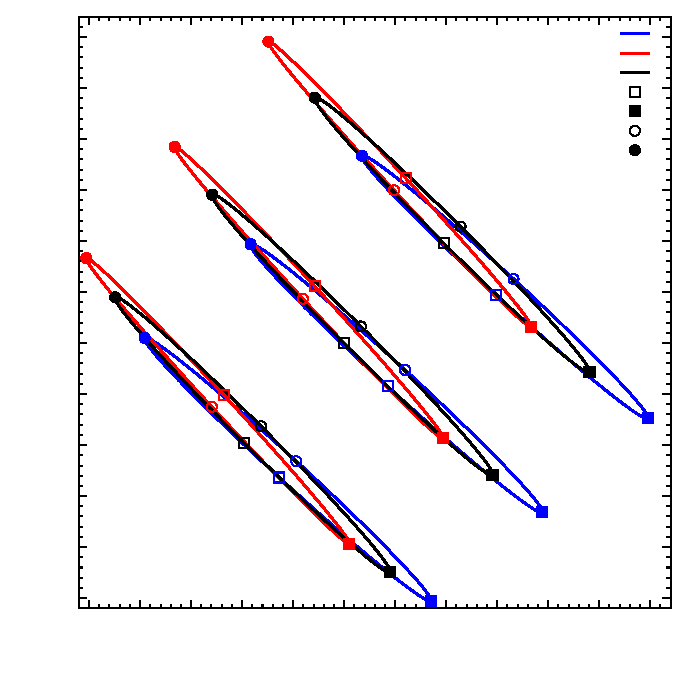
\includegraphics{pics/base_ball}}%
    \gplfronttext
  \end{picture}%
\endgroup
}
	\hfill
	\raisebox{2em}{\resizebox{0.52\linewidth}{!}{% GNUPLOT: LaTeX picture with Postscript
\begingroup
  \makeatletter
  \providecommand\color[2][]{%
    \GenericError{(gnuplot) \space\space\space\@spaces}{%
      Package color not loaded in conjunction with
      terminal option `colourtext'%
    }{See the gnuplot documentation for explanation.%
    }{Either use 'blacktext' in gnuplot or load the package
      color.sty in LaTeX.}%
    \renewcommand\color[2][]{}%
  }%
  \providecommand\includegraphics[2][]{%
    \GenericError{(gnuplot) \space\space\space\@spaces}{%
      Package graphicx or graphics not loaded%
    }{See the gnuplot documentation for explanation.%
    }{The gnuplot epslatex terminal needs graphicx.sty or graphics.sty.}%
    \renewcommand\includegraphics[2][]{}%
  }%
  \providecommand\rotatebox[2]{#2}%
  \@ifundefined{ifGPcolor}{%
    \newif\ifGPcolor
    \GPcolortrue
  }{}%
  \@ifundefined{ifGPblacktext}{%
    \newif\ifGPblacktext
    \GPblacktexttrue
  }{}%
  % define a \g@addto@macro without @ in the name:
  \let\gplgaddtomacro\g@addto@macro
  % define empty templates for all commands taking text:
  \gdef\gplbacktext{}%
  \gdef\gplfronttext{}%
  \makeatother
  \ifGPblacktext
    % no textcolor at all
    \def\colorrgb#1{}%
    \def\colorgray#1{}%
  \else
    % gray or color?
    \ifGPcolor
      \def\colorrgb#1{\color[rgb]{#1}}%
      \def\colorgray#1{\color[gray]{#1}}%
      \expandafter\def\csname LTw\endcsname{\color{white}}%
      \expandafter\def\csname LTb\endcsname{\color{black}}%
      \expandafter\def\csname LTa\endcsname{\color{black}}%
      \expandafter\def\csname LT0\endcsname{\color[rgb]{1,0,0}}%
      \expandafter\def\csname LT1\endcsname{\color[rgb]{0,1,0}}%
      \expandafter\def\csname LT2\endcsname{\color[rgb]{0,0,1}}%
      \expandafter\def\csname LT3\endcsname{\color[rgb]{1,0,1}}%
      \expandafter\def\csname LT4\endcsname{\color[rgb]{0,1,1}}%
      \expandafter\def\csname LT5\endcsname{\color[rgb]{1,1,0}}%
      \expandafter\def\csname LT6\endcsname{\color[rgb]{0,0,0}}%
      \expandafter\def\csname LT7\endcsname{\color[rgb]{1,0.3,0}}%
      \expandafter\def\csname LT8\endcsname{\color[rgb]{0.5,0.5,0.5}}%
    \else
      % gray
      \def\colorrgb#1{\color{black}}%
      \def\colorgray#1{\color[gray]{#1}}%
      \expandafter\def\csname LTw\endcsname{\color{white}}%
      \expandafter\def\csname LTb\endcsname{\color{black}}%
      \expandafter\def\csname LTa\endcsname{\color{black}}%
      \expandafter\def\csname LT0\endcsname{\color{black}}%
      \expandafter\def\csname LT1\endcsname{\color{black}}%
      \expandafter\def\csname LT2\endcsname{\color{black}}%
      \expandafter\def\csname LT3\endcsname{\color{black}}%
      \expandafter\def\csname LT4\endcsname{\color{black}}%
      \expandafter\def\csname LT5\endcsname{\color{black}}%
      \expandafter\def\csname LT6\endcsname{\color{black}}%
      \expandafter\def\csname LT7\endcsname{\color{black}}%
      \expandafter\def\csname LT8\endcsname{\color{black}}%
    \fi
  \fi
    \setlength{\unitlength}{0.0500bp}%
    \ifx\gptboxheight\undefined%
      \newlength{\gptboxheight}%
      \newlength{\gptboxwidth}%
      \newsavebox{\gptboxtext}%
    \fi%
    \setlength{\fboxrule}{0.5pt}%
    \setlength{\fboxsep}{1pt}%
\begin{picture}(7200.00,5040.00)%
    \gplgaddtomacro\gplbacktext{%
      \csname LTb\endcsname%%
      \put(645,595){\makebox(0,0)[r]{\strut{}-50}}%
      \csname LTb\endcsname%%
      \put(645,1021){\makebox(0,0)[r]{\strut{}-40}}%
      \csname LTb\endcsname%%
      \put(645,1447){\makebox(0,0)[r]{\strut{}-30}}%
      \csname LTb\endcsname%%
      \put(645,1872){\makebox(0,0)[r]{\strut{}-20}}%
      \csname LTb\endcsname%%
      \put(645,2298){\makebox(0,0)[r]{\strut{}-10}}%
      \csname LTb\endcsname%%
      \put(645,2724){\makebox(0,0)[r]{\strut{}0}}%
      \csname LTb\endcsname%%
      \put(645,3150){\makebox(0,0)[r]{\strut{}10}}%
      \csname LTb\endcsname%%
      \put(645,3576){\makebox(0,0)[r]{\strut{}20}}%
      \csname LTb\endcsname%%
      \put(645,4001){\makebox(0,0)[r]{\strut{}30}}%
      \csname LTb\endcsname%%
      \put(645,4427){\makebox(0,0)[r]{\strut{}40}}%
      \csname LTb\endcsname%%
      \put(645,4853){\makebox(0,0)[r]{\strut{}50}}%
      \csname LTb\endcsname%%
      \put(747,409){\makebox(0,0){\strut{}-1.00$\pi$}}%
      \csname LTb\endcsname%%
      \put(1515,409){\makebox(0,0){\strut{}-0.75$\pi$}}%
      \csname LTb\endcsname%%
      \put(2284,409){\makebox(0,0){\strut{}-0.50$\pi$}}%
      \csname LTb\endcsname%%
      \put(3052,409){\makebox(0,0){\strut{}-0.25$\pi$}}%
      \csname LTb\endcsname%%
      \put(3820,409){\makebox(0,0){\strut{}0.00$\pi$}}%
      \csname LTb\endcsname%%
      \put(4588,409){\makebox(0,0){\strut{}0.25$\pi$}}%
      \csname LTb\endcsname%%
      \put(5357,409){\makebox(0,0){\strut{}0.50$\pi$}}%
      \csname LTb\endcsname%%
      \put(6125,409){\makebox(0,0){\strut{}0.75$\pi$}}%
      \csname LTb\endcsname%%
      \put(6893,409){\makebox(0,0){\strut{}1.00$\pi$}}%
    }%
    \gplgaddtomacro\gplfronttext{%
      \csname LTb\endcsname%%
      \put(153,2724){\rotatebox{-270}{\makebox(0,0){\strut{}Normalised asymmetry $\mathcal{A}$ (\%)}}}%
      \csname LTb\endcsname%%
      \put(3820,130){\makebox(0,0){\strut{}$\delta_\text{CP}$}}%
      \csname LTb\endcsname%%
      \put(6309,4686){\makebox(0,0)[r]{\strut{}Normal hierarchy}}%
      \csname LTb\endcsname%%
      \put(6309,4500){\makebox(0,0)[r]{\strut{}Inverted hierarchy}}%
      \csname LTb\endcsname%%
      \put(6309,4314){\makebox(0,0)[r]{\strut{}Vacuum}}%
    }%
    \gplbacktext
    \put(0,0){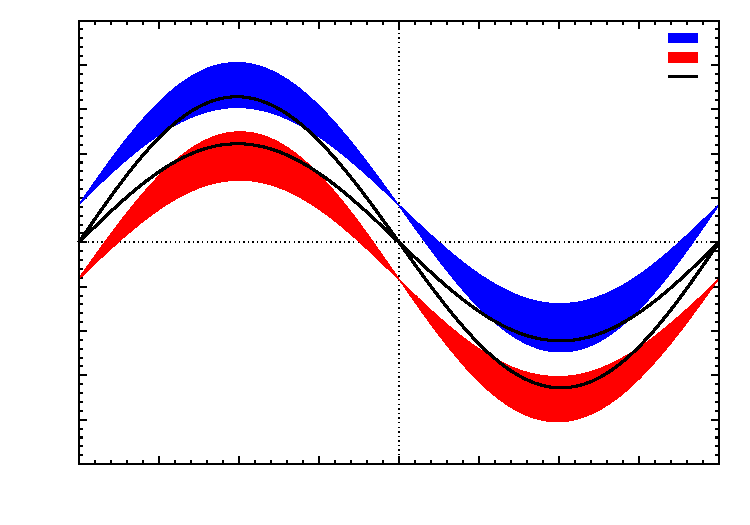
\includegraphics{pics/norm_asymm}}%
    \gplfronttext
  \end{picture}%
\endgroup
}}
	\caption[Effect of $\delta_\text{CP}$ on the oscillation probability]%
		{Effect of $\delta_\text{CP}$ on the oscillation probability.
		The oscillation probabilities for neutrinos and antineutrinos are plotted %
		against each other (left), while the CP phase is varied between $-\pi$ and $\pi$.
		The effect of $\sin^2\theta_{23}$ is also emphasised.
		The mass hierarchy has a nonnegligible behaviour only if matter oscillation is %
		considered.
		The normalised asymmetry from Eq.~\ref{eq:asymmetry} is shown on the right.
		When not specified, both graphs are created with the Design Report oscillation parameters (see \reftab{tab:asimovA}).
		A neutrino energy of 0.6\,GeV and a baseline of 295\,km was used to calculate the oscillation probability.}
	\label{fig:baseball}
\end{figure}

Given the parametrisation in Eq.~\ref{eq:pmns}, %
it is clear that the asymmetry is not measurable if the phase is trivial, \ie~$\delta_\text{CP} = 0$~or~$\pm \pi$, %
or if $\theta_{13}$ is vanishing.
From a model building point of view, however, a successful leptogenesis requires the parameters to satisfy %
$\qty|\sin\theta_{13} \sin\delta_\text{CP}| \gtrsim 0.09$
%\begin{equation}
%	\label{eq:leptogenesis}
%	\qty|\sin\theta_{13} \sin\delta_\text{CP}| \gtrsim 0.09\ ,
%\end{equation}
when the Majorana phases are vanishing~\cite{Pascoli:2006ci}.
The value of $\theta_{13}$ has been measured to be nonzero~\cite{Abe:2011sj,Abe:2011fz,An:2012eh,Ahn:2012nd} %
and for this reason it is expected that ongoing and future generation neutrino experiments %
will constrain the value of $\delta_\text{CP}$.


\section{Hyper-Kamiokande experiment}
\label{sec:hk}

\begin{figure}
	\centering
	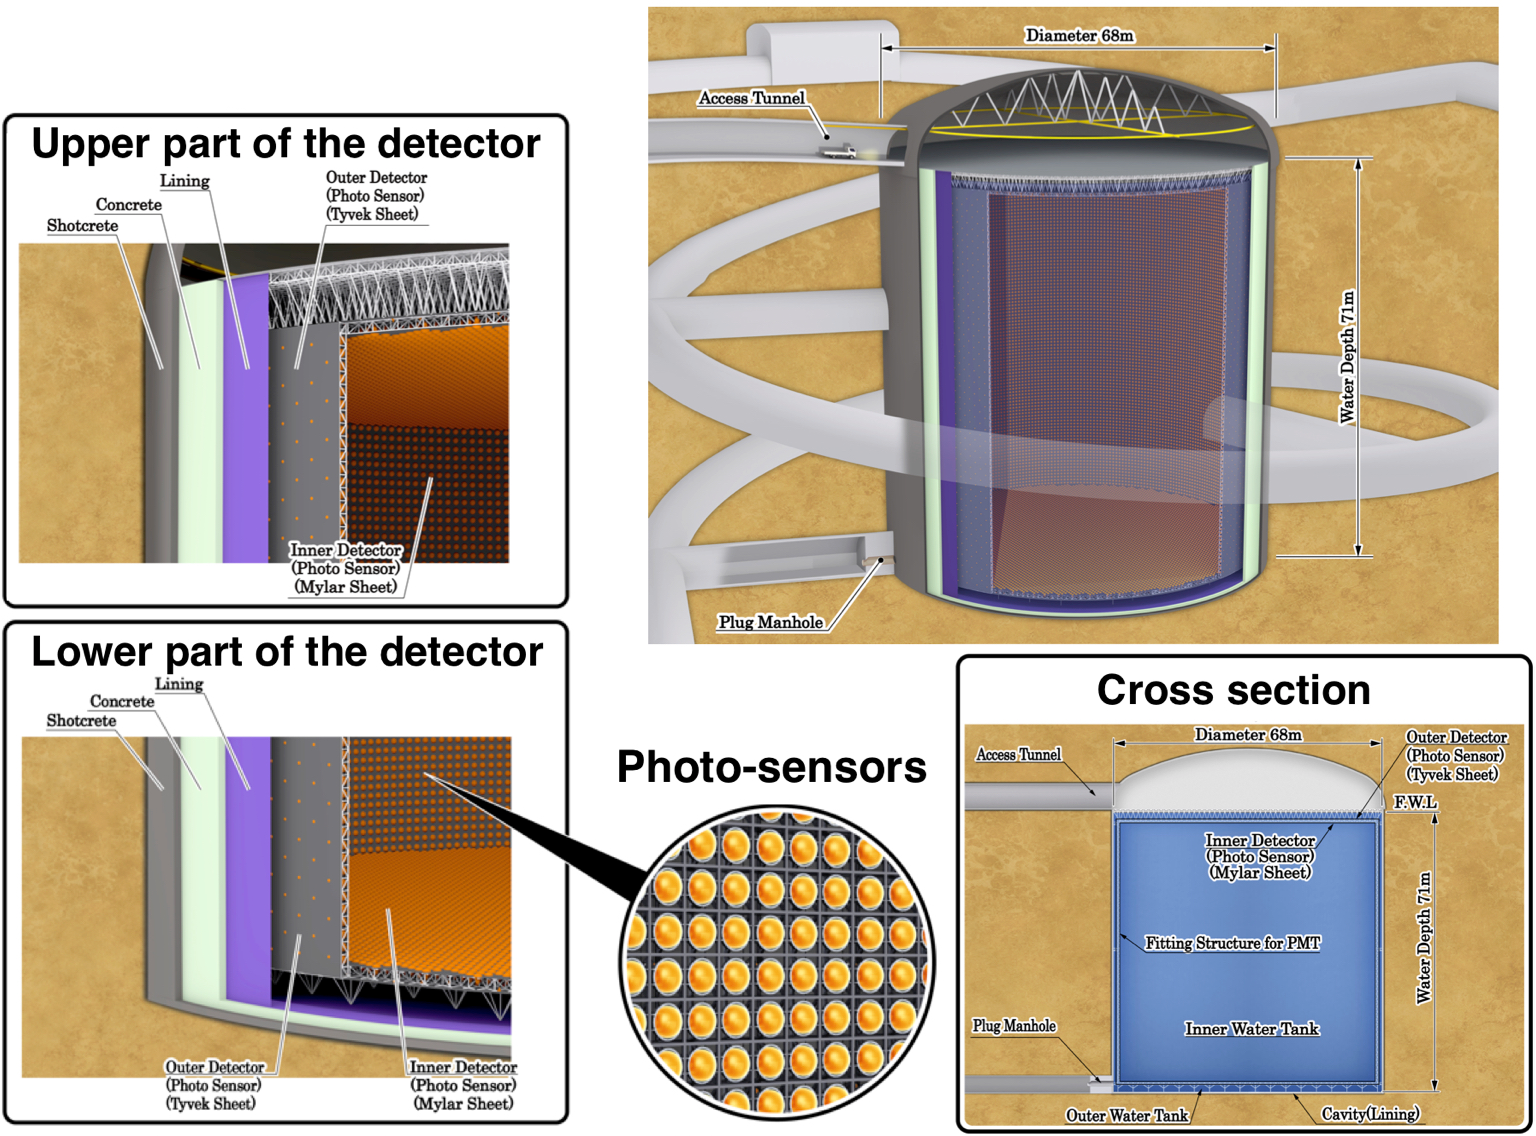
\includegraphics[width=0.8\linewidth]{pics/hkonlytank.png}
	\caption[Views of the Hyper-Kamiokande experiment]{Cut-views of the Hyper-Kamiokande experiment.}
	\label{fig:hkdr}
\end{figure}

Hyper-Kamiokande (HK)~\cite{Abe:2018uyc} will be the next-generation water Cherenkov detector, %
studying neutrino interactions and searching for nucleon decays with the ring-imaging technique.
The detector will be located in the Tochibora mine, under Mt.\ Nijugo in the Gifu Prefecture, Japan, 
just 8\,km south from Super-Kamiokande.
At this location, the rock overburden is equivalent to 1750\,m.w.e.
%superseding its predecessor, Super-Kamiokande (SK).
%, the rare interactions of neutrinos can be detected, %
%as well as the possible spontaneous decay of nucleons.
The design of HK is similar to the one of SK and Kamiokande, with size being the biggest difference.
The cylindrical tank of HK will be 72\,m high and 68\,m in diameter, with a fiducial volume of 188.4\,kton (total volume 257.8\,kton), %
around 8.4 times the fiducial volume of SK.
The photo-coverage of the inner detector region will be 40\,\%, the same of SK, %
but it translates to roughly forty thousand photomultipliers (PMTs).
New 20'' box and line PMTs will be employed, with improved charge and timing resolution, %
and an increased quantum efficiency which is almost twice as much that of the previous generation of PMTs.
The new photosensors must also have a high pressure tolerance to be used at a depth of 60\,m and more of water.
A study for implementing multi PMT modules, containing each 23 3'' PMT, is also being carried out.
%The detector will be located underground at Kamioka mine in Gifu Prefecture, %
%with an overburden of approximately 650 meters or more of rock, which is equivalent to \np{1750} meters or more of water.
As SK, the new detector will have an outer detector which is just 1\,m wide and instrumented with 3'' PMTs.
Thanks to incredible statistics and cutting edge resolutions, HK will be capable of a vast variety of physics studies, %
from accelerator and atmospheric neutrinos to solar and supernova neutrinos.
Besides detecting proton decay, the main goal of HK is to measure~$\delta_\text{CP}$ and constrain the other oscillation parameters %
with high precision.
This is best achieved by studying accelerator neutrinos which allow a higher control of the experimental variables, %
and to this end the possibility of installing a second detector in Korea %
at the secondary oscillation peak is being investigated by the collaboration.

HK will be located 295\,km away from the T2K target and at $2.5^\circ$ off-axis with respect to the beamline.
The neutrino beam is generated by a 30\,GeV proton beam in the way described in \refsec{sec:nu_acc}.
By selecting the direction of the horn's current, an almost pure muon neutrino (or antineutrino) beam is obtained, peaking at 600\,MeV.
The accelerator facility at J-PARC will undergo a planned upgrade to increase the beam power to 1.3\,MW, %
before HK starts operation.
The T2K near detector system, consisting of the detectors ND280 ($2.5^\circ$ off-axis) and INGRID (on-axis)~\cite{Abe:2011ks}, %
will be refurbished and a new near detector, called \emph{Intermediate Water Cherenkov Detector}, possibly gadolinium-loaded, %
will be located around 1\,km from the target.
HK will take data for ten years, collecting a total of \np{2.7e22} protons on target (POT), %
divided between $\nu$ and $\cj{\nu}$ beam modes.
Studies have shown that CP violation discovery is not very sensitive to POT allocation between the two modes~\cite{Abe:2018uyc}.
Assuming a POT ratio $\nu:\cj{\nu} = 1:3$ and $\delta_\text{CP} = 0$, %
the expected number of fully-contained events in the fiducial volume for the channels %
$\nu_\mu \to \nu_e$ and $\cj{\nu}_\mu \to \cj{\nu}_e$ %
are respectively \np{1643} and \np{15} in $\nu$ mode and \np{206} and \np{1183} in $\cj{\nu}$ mode, %
assuming CP conservation.
Deviations from these expected numbers could be an indication of CP violation.
%A preliminary study for the HK design report~\cite{Abe:2018uyc}, using a different analysis, %
%estimated a significance well-above $5\,\sigma$ after ten years of data taking, as can be seen in Fig.~\ref{fig:hkdr}.
The project has been recently approved by the Japanese government and data taking is expected to start in 2027.

%The uncertainty of the Earth’s density between Tokai and Kamioka is estimated to be at most 6\% [181].
%Because the matter effect contribution to the total $\nu_\mu \to \nu_e$ appearance probability is %
%less than 10\% for 295km baseline, the uncertainty from the matter density is estimated to be less
%than 0.6\% and neglected in the following analysis.


\section{Sensitivity studies}
\label{sec:sensitivity}

At any stage of the experiment it is important to asses the impact of systematic errors on the total sensitivity of HK.
%One of the main goal is to constrain with high precision oscillation parameters, especially $\delta_\text{CP}$ %
%and the $\theta_{23}$ octant.
Even if real data is not available, it is possible to understand whether the planned volume of data to be collected %
has enough constraining power to achieve the target precision.
The oscillation and systematic parameters are input to a Monte Carlo simulation %
to build the expected distribution of events.
This expected data is then compared to simulated ``observed data'', which is created by selecting %
a combination of oscillation parameters in order to mimic the real distributions of events that will be eventually collected.
Scanning over the oscillation parameters, the resolution of HK to oscillation parameters and, more importantly, %
the influence of the systematic uncertainties can be studied.
To this end, a fitting framework capable of performing a simultaneous study of beam and atmospheric samples was employed. 

\subsection{Event samples}
\label{sec:event_samples}

\begin{table}[t]
	\centering
	\caption[Sample events for atmospheric data]%
		{The sample events for atmospheric data are used to build 2D distributions in $\log p$ and $\cos\theta$.
		The number of bins in each direction is listed and they sum up to 2224.
		The samples are categorised as fully-contained sub-GeV (FC sub-GeV), %
		fully-contained multi-GeV (FC multi-GeV), partially-contained (PC) and upward-going muons (UP-$\mu$).}
	\label{tab:atmo_samples}
	\small
	\begin{tabular}{llcc}
		\toprule
		Event type	&	Sample	&	Bins $\log p$	& Bins $\cos\theta$  \\
		\midrule
		\multirow{7}{*}{\bf FC sub-GeV}	& one ring $e$-like and 0 decay-$e$	& 13 & 20 \\
						& one ring $e$-like and 1 decay-$e$	& 13 & 1 \\
						& one ring $\mu$-like and 0 decay-$e$	& 13 & 20 \\
						& one ring $\mu$-like and 1 decay-$e$	& 13 & 20\\
						& one ring $\mu$-like and 2 decay-$e$	& 13 & 1 \\
						& one ring $\pi^0$			& 13 & 1 \\
						& two rings $\pi^0$			& 5 & 1 \\
		\midrule
		\multirow{7}{*}{\bf FC multi-GeV}& one ring $e$-like ($\nu_e$) 	& 10 & 20 \\
						& one ring $e$-like ($\cj{\nu}_e$) & 10 & 20 \\
						& one ring $\mu$-like           & 5 & 20 \\
						& multi ring $e$-like ($\nu_e$) & 8 & 20 \\
						& multi ring $e$-like ($\cj{\nu}_e$) & 8 & 20 \\
						& multi ring $\mu$-like	        & 4 & 20 \\
						& multi ring other		& 10 & 20 \\
		\midrule
		\multirow{2}{*}{\bf PC}		& stopping 			& 4 & 20 \\
						& through-going 		& 5 & 20 \\
		\midrule
		\multirow{3}{*}{\bf UP-$\mu$}	& stopping 			& 4 & 20 \\
						& through-going, not showering 	& 1 & 20 \\
						& through-going, showering 	& 1 & 20 \\
		\bottomrule
	\end{tabular}
\end{table}

For the study, SK atmospheric Monte Carlo (MC) data are adapted and scaled to HK statistics to form the atmospheric sample.
The events are then classified and binned into several two-dimensional histograms of $\log p$ and $\cos\vartheta$, %
where $p$ and $\vartheta$ are respectively the momentum and the azimuthal angle of the reconstructed charged lepton.
The histograms are summarised in~\reftab{tab:atmo_samples} where they are categorised as fully-contained (FC), %
partially-contained (PC), or upward-going muons (UP-$\mu$) events~\cite{Jiang:2019xwn}.
There are a total of \np{2224} bins employed for the atmospheric sample.
The beam sample instead is created using the far detector flux prediction, as explained in \refsec{sec:prediction}.
From the flux prediction, fully-contained candidate events in the fiducial volume are grouped %
as appearance signal, i.e.\ $\nu_\mu\to\nu_e$ and $\cj{\nu}_\mu\to\cj{\nu}_e$, %
and background events from disappearance channels.
Signal and background distributions in true energy (98 bins) undergo event selection criteria %
to obtain the distributions in reconstructed energy (87 bins) for the four event samples: %
one ring $e$-like in $\nu$-mode; %
one ring $\mu$-like in $\nu$-mode; %
one ring $e$-like in $\cj{\nu}$-mode; %
one ring $\mu$-like in $\cj{\nu}$-mode.
A set of 2D smearing matrices, produced by the T2K fitting framework VALOR~\cite{VALOR}, %
simulates and replaces the correct event selection process, including tuning of the flux with near detector constraints.
These smearing matrices are provided for all samples, acting on signal (CCQE and CCnQE) %
and background (CCQE, CCnQE, and NC) distributions.
The one ring $e$-like with one electron decay sample is not considered in this study.




\subsection{Oscillation space}
\label{sec:osc_space}

\begin{table}
	\small
	\centering
	\caption[Parameter space used in the oscillation analysis]%
		{The oscillation parameter sets used in this thesis are shown here.
		The reference set ``Design'' is taken from the HK design report~\cite{Abe:2018uyc}.
		The sensitivity studies are carried out in a parameters space built around ``Asimov A'', %
		the nominal T2K best fit point~\cite{Abe:2018wpn}.
		It spans over the four parameters $\Delta m_{23}^2$, $\sin^2 2\theta_{13}$, %
		$\sin^2 \theta_{23}$, and $\delta_\text{CP}$, whereas $\Delta m_{12}$ and $\sin^2 2\theta_{12}$ %
		are fixed. The range and number of points scanned are reported in the last two columns.}

	\label{tab:asimovA}
	\begin{tabular}{ccccc}
		\toprule
		Parameter				& Design & Asimov A	& Range	& Points \\
		\midrule
		$\Delta m_{12}^2/\np{e-5}\,\text{eV}^2$	& 7.60	& 7.53		& --			& fixed	\\
		$\sin^2 2\theta_{12}$			& 0.8704 & 0.8463	& --			& fixed	\\
		\midrule
		$\Delta m_{23}^2/\np{e-3}\,\text{eV}^2$	& 2.4	& 2.509		& [2.464:2.554]		& 13	\\
		$\sin^2 2\theta_{13}$			& 0.1	& 0.085		& [0.070:0.100]		& 13	\\
		$\sin^2 \theta_{23}$			& 0.5 	& 0.528		& [0.426:0.579]		& 19	\\
		$\delta_\text{CP}$			& 0	& $-\pi/2$	& [$-\pi$:$\pi$]	& 61	\\
		\bottomrule
	\end{tabular}
\end{table}


Both the atmospheric and beam distributions are weighted by the corresponding oscillation probabilities.
The oscillation parameters are scanned over the space defined by the four variables %
\begin{equation}
	\Delta m^2_{32} \times \sin^2 2\theta_{13} \times \sin^2 \theta_{23} \times \delta_\text{CP}
\end{equation}
on a grid of respectively $13\,\times\,13\,\times\,19\,\times\,61$ points.
The solar squared mass difference and the solar angle $\theta_{12}$ are fixed.
Apart from $\delta_\text{CP}$ which is scanned over all possible values, %
the intervals for the other parameters are built around ``Asimov A'', the best fit point used by T2K %
for Asimov and fake data studies~\cite{Abe:2018wpn} .
The details of the oscillation space are listed in \reftab{tab:asimovA}.
For the atmospheric squared mass difference and $\sin^2 2\theta_{13}$, the range is chosen such that it covers %
a $[-3\sigma, +3\sigma]$ interval, where $\sigma$ is the error from the Asimov A set; %
the range for $\sin^2\theta_{23}$ spans over $[-6\sigma, +3\sigma]$ so that both octants are covered symmetrically.
%Reactor experiments~\cite{Bak:2018ydk, Adey:2018zwh}.
At each point of this space, the event distributions are weighted with the correct oscillation probability %
for appearance or disappearance channels.
The Asimov A point is chosen to be the \emph{true} combination of oscillation parameters %
to perform sensitivity studies using a $\chi^2$-test statistic.
By changing the \emph{true} value of the CP phase, it is possible to define the exclusion regions for CP conservation, %
by comparing the $\chi^2$ at any value of $\delta_\text{CP}$ with the $\chi^2$ computed at %
the null hypothesis, i.e.\ CP conservation or $\delta_\text{CP} = 0, \pm\pi$.
The exclusion sensitivity as a function of \emph{true} $\delta_\text{CP}$ %
is quantified by %
\begin{equation}
	\sigma = \sqrt{\min_{\delta_\text{CP} = 0,\pm\pi}\! \chi^2\  -\,\chi^2_\text{\emph{true}}}\ ,
\end{equation}
where $\chi^2_\text{\emph{true}}$ is evaluated at the \emph{true} point and matches the best fit value.
The normal hierarchy is assumed to be known, except where stated.



\subsection{Test statistic}
\label{sec:x2}

Let us define the likelihood
\begin{equation}
	\mathfrak{L}(E_n, O_n) = \prod_n \frac{e^{-E_n} E_n^{O_n}}{O_n!}\ ,
\end{equation}
where $O_n$ and $E_n$ are respectively the number of observed and expected events in the $n$-th bin, %
which are built using a combination of oscillation parameters 
\begin{equation}
	\Theta = (\Delta m^2_{32}, \sin^2 2\theta_{13}, \sin^2 \theta_{23}, \delta_\text{CP})\ .
\end{equation}
The expected events are defined by a prediction of events at the far detector weighted by the oscillation probabilities %
for parameters $\Theta$, and since there is no real data yet the ``observed'' events are also given by %
a prediction at the \emph{true} oscillation point $\Theta_\text{true}$.
%and the product runs over the total number of bins.
The $\chi^2$ is hence the following log-likelihood ratio
\begin{equation}
	\label{eq:log_ratio}
	\chi^2(\Theta) = -2 \log \qty[\frac{\mathfrak{L}(E_n, O_n)}{\mathfrak{L}(O_n, O_n)}] =
		2 \sum_n \qty[E_n - O_n + O_n \log \qty(\frac{O_n}{E_n})]\ ,
\end{equation}
which is modified according to the ``pull approach'' $\chi^2$~\cite{Fogli:2002pt}: %
the parameters $\bs{\varepsilon} = \{\varepsilon_j\}$ are introduced %
to account for systematic uncertainties by replacing
\begin{equation}
	\label{eq:pull}
	E_n\ \longrightarrow\ E_n\,\qty(1 + \textstyle\sum_j f_j^n \varepsilon_j)\ ,
\end{equation}
where the index $j$ runs over the systematic parameters.
A penalty term that includes variances and covariances of such parameters is added to the likelihood, %
using the inverse of the correlation matrix of the systematic errors, $\rho^{-1}$.
With all these adjustments included, the $\chi^2$ becomes
%\begin{align}
%	\chi^2_\text{tot} &=\ \chi^2_\text{obs}\ +\ \chi^2_\text{syst} \notag\\
%	&= \overset{\text{obs}}{2 \sum_n \qty[E_n(1+{\textstyle\sum_j f_j^n \varepsilon_j}) - O_n + O_n \log \qty(\frac{E_n(1+\sum_j f_j^n \varepsilon_j)}{O_n})]} + %
%	\overset{\text{\shortstack{syst\\ \hphantom{.}}}}{\sum_{ij} \varepsilon_i\, \rho^{-1}_{ij}\, \varepsilon_j}\ ,
%\end{align}
\begin{align}
	\chi^2(\Theta;\bs{\varepsilon})  =&\ 2 \sum_n \qty[E_n(1+{\textstyle\sum_j f_j^n \varepsilon_j}) - O_n + %
		O_n \log \qty(\frac{O_n}{E_n(1+\sum_j f_j^n \varepsilon_j)})] \notag \\
	\label{eq:chi2}
		&+ \sum_{ij} \varepsilon_i\, \rho^{-1}_{ij}\, \varepsilon_j\ .
\end{align}
The effect of the systematic uncertainties on the event distributions are embedded in the $f_j^n$ parameters, %
defined as the fractional change induced on the $n$-th bin by a 1\,$\sigma$ variation of the $j$-th systematic.
The amount of change is therefore parameterised by the $\varepsilon_j$ in units of the uncertainty $\sigma_j$.
However, being $\rho$ the correlation matrix, the $\varepsilon_j$ are promoted to embody the systematic uncertainties.
Once the observed sample is defined, the oscillation parameters $\Theta$ are scanned over the oscillation %
space defined in \reftab{tab:asimovA} to estimate the expected events; finally, the $\chi^2$ is profiled %
with respect to the parameters~$\bs{\varepsilon}$:
\begin{equation}
	\label{eq:chi2_min}
	\chi^2(\Theta) = \min_{\bs{\varepsilon}}\, \qty\Big[\,\chi^2(\Theta;\bs{\varepsilon})\,]\ .
\end{equation}
Fixing the combination $\Theta$ and dropping it from the notation, %
the minimisation of the $\chi^2$ leads to the following set of $j$ nonlinear equations %,
\begin{equation}
	\pdv{\chi^2}{\varepsilon_j} (\bs{\varepsilon}) = 0\ 
\end{equation}
which can be solved iteratively if the condition $\sum_j f^n_j \varepsilon_j < 1$~holds.
The system can then be solved with the Gauss-Newton's method by finding the Hessian of the $\chi^2$.
This gives a linear system, which can be solved iteratively until convergence on $\varepsilon_j$ is achieved:
%The algorithm is stabilised by means of the Levenberg-Marquardt algorithm
\begin{equation}
	\pdv{\chi^2(\bs{\varepsilon}^{(n)})}{\varepsilon_k}{\varepsilon_j} %
	\cdot \qty(\varepsilon_j^{(n+1)} - \varepsilon_j^{(n)}) = %
	-\pdv{\chi^2(\bs{\varepsilon}^{(n)})}{\varepsilon_k}\ ,
\end{equation}
with $(n)$ the iteration index.
The Gauss-Newton's algorithm can sometimes be unstable, especially with a large number of parameters, %
due to its fast convergence.
The algorithm is typically improved by adopting the Lavenberg-Marquardt method~\cite{Levenberg_1944, Marquardt_1963} %
which modifies the Hessian and the equations become
\begin{equation}
	\qty[\pdv{\chi^2(\bs{\varepsilon}^{(n)})}{\varepsilon_k}{\varepsilon_j} %
	+ \lambda \max \qty(\text{diag} \pdv{\chi^2(\bs{\varepsilon}^{(n)})}{\varepsilon_k}{\varepsilon_j}) \mathbb{1}]
	\cdot \qty(\varepsilon_j^{(n+1)} - \varepsilon_j^{(n)}) = %
	-\pdv{\chi^2(\bs{\varepsilon}^{(n)})}{\varepsilon_k}\ .
\end{equation}
The parameter $\lambda$ is chosen dynamically: if the cost function $\chi^2$ decreases %
after an iteration step, then $\lambda$ is reduced; otherwise $\lambda$ is increased and the step recomputed.
In the limit $\lambda \to 0$, the algorithm approximates the Gauss-Newton's method and its fast convergence.
When $\lambda$ is large, the linear system resembles a gradient descent with small steps of the order of $\lambda^{-1}$, %
but with a more stable convergence.
A ``delayed-gratification scheme'' is adopted for $\lambda$~\cite{Transtrum2012}, using an initial value of $\lambda^{(0)} = 1$ and finding %
an optimal increment and decrement of respectively $\lambda^{(n+1)} = 5\,\lambda^{(n)}$ and $\lambda^{(n+1)} = \lambda^{(n)} / 10$.

To account for future constraints from other experiments, a Gaussian penalty term is added %
to the minimised value of $\chi^2$ from \refeq{eq:chi2_min}
\begin{equation}
	\chi^2_\text{penalty} = \frac{(\Theta - \hat{\Theta})^2}{\sigma_\Theta^2}\ .
\end{equation}
In this analysis, only the error on $\theta_{13}$ is considered %
which is predicted to be $\sigma(\sin^2 2\theta_{13}) = 0.005$ from measurements of reactor experiments.

For most of the systematic parameters, a linear response is assumed in the~MC.
This means that varying the $j$-th systematic by a known amount, $\beta_j \to \beta_j + \varepsilon_j\sigma_j$ %
the number of expected events changes accordingly:
\begin{equation}
	\label{eq:linear}
	\beta_j\ \overset{\scriptstyle \text{MC}}{\longmapsto}\ E_n %
	%\qquad \overset{\varepsilon_j \sigma_j}{\Longrightarrow} \qquad %
	\qquad \Longrightarrow \qquad %
	\beta_j + \varepsilon_j\sigma_j\ \overset{\text{MC}}{\longmapsto}\ E_n ( 1 + \varepsilon_j f_n ^j )\ .
	%&\hspace{0.4em}\text{\scriptsize MC} \\
	%\text{\scriptsize MC\ :} \hspace{1em} \Downarrow & \hspace{3.5em} \Downarrow	\\	
\end{equation}
Certain systematic uncertainties, such as the CCQE axial-mass scaling factor, the Fermi momentum for \tapi{16}O, %
or some of the RPA coefficients, %
%\footnote{The Random Phase Approximation (RPA) method is applied to calculate the total cross-sections %
	%of electron neutrinos on nuclei.}, 
do not present a linear behaviour for small values of $\varepsilon$ %
and they are better described by a four-point linear interpolation of different~$f_j^n$ histograms, %
computed at~$\pm1\,\sigma$ and~$\pm3\,\sigma$ variations of the systematic parameter.




\subsection{Far detector prediction}
\label{sec:prediction}

\begin{figure}[t]
	\centering
	\resizebox{0.49\linewidth}{!}{% GNUPLOT: LaTeX picture with Postscript
\begingroup
  \makeatletter
  \providecommand\color[2][]{%
    \GenericError{(gnuplot) \space\space\space\@spaces}{%
      Package color not loaded in conjunction with
      terminal option `colourtext'%
    }{See the gnuplot documentation for explanation.%
    }{Either use 'blacktext' in gnuplot or load the package
      color.sty in LaTeX.}%
    \renewcommand\color[2][]{}%
  }%
  \providecommand\includegraphics[2][]{%
    \GenericError{(gnuplot) \space\space\space\@spaces}{%
      Package graphicx or graphics not loaded%
    }{See the gnuplot documentation for explanation.%
    }{The gnuplot epslatex terminal needs graphicx.sty or graphics.sty.}%
    \renewcommand\includegraphics[2][]{}%
  }%
  \providecommand\rotatebox[2]{#2}%
  \@ifundefined{ifGPcolor}{%
    \newif\ifGPcolor
    \GPcolortrue
  }{}%
  \@ifundefined{ifGPblacktext}{%
    \newif\ifGPblacktext
    \GPblacktexttrue
  }{}%
  % define a \g@addto@macro without @ in the name:
  \let\gplgaddtomacro\g@addto@macro
  % define empty templates for all commands taking text:
  \gdef\gplbacktext{}%
  \gdef\gplfronttext{}%
  \makeatother
  \ifGPblacktext
    % no textcolor at all
    \def\colorrgb#1{}%
    \def\colorgray#1{}%
  \else
    % gray or color?
    \ifGPcolor
      \def\colorrgb#1{\color[rgb]{#1}}%
      \def\colorgray#1{\color[gray]{#1}}%
      \expandafter\def\csname LTw\endcsname{\color{white}}%
      \expandafter\def\csname LTb\endcsname{\color{black}}%
      \expandafter\def\csname LTa\endcsname{\color{black}}%
      \expandafter\def\csname LT0\endcsname{\color[rgb]{1,0,0}}%
      \expandafter\def\csname LT1\endcsname{\color[rgb]{0,1,0}}%
      \expandafter\def\csname LT2\endcsname{\color[rgb]{0,0,1}}%
      \expandafter\def\csname LT3\endcsname{\color[rgb]{1,0,1}}%
      \expandafter\def\csname LT4\endcsname{\color[rgb]{0,1,1}}%
      \expandafter\def\csname LT5\endcsname{\color[rgb]{1,1,0}}%
      \expandafter\def\csname LT6\endcsname{\color[rgb]{0,0,0}}%
      \expandafter\def\csname LT7\endcsname{\color[rgb]{1,0.3,0}}%
      \expandafter\def\csname LT8\endcsname{\color[rgb]{0.5,0.5,0.5}}%
    \else
      % gray
      \def\colorrgb#1{\color{black}}%
      \def\colorgray#1{\color[gray]{#1}}%
      \expandafter\def\csname LTw\endcsname{\color{white}}%
      \expandafter\def\csname LTb\endcsname{\color{black}}%
      \expandafter\def\csname LTa\endcsname{\color{black}}%
      \expandafter\def\csname LT0\endcsname{\color{black}}%
      \expandafter\def\csname LT1\endcsname{\color{black}}%
      \expandafter\def\csname LT2\endcsname{\color{black}}%
      \expandafter\def\csname LT3\endcsname{\color{black}}%
      \expandafter\def\csname LT4\endcsname{\color{black}}%
      \expandafter\def\csname LT5\endcsname{\color{black}}%
      \expandafter\def\csname LT6\endcsname{\color{black}}%
      \expandafter\def\csname LT7\endcsname{\color{black}}%
      \expandafter\def\csname LT8\endcsname{\color{black}}%
    \fi
  \fi
    \setlength{\unitlength}{0.0500bp}%
    \ifx\gptboxheight\undefined%
      \newlength{\gptboxheight}%
      \newlength{\gptboxwidth}%
      \newsavebox{\gptboxtext}%
    \fi%
    \setlength{\fboxrule}{0.5pt}%
    \setlength{\fboxsep}{1pt}%
\begin{picture}(7200.00,5040.00)%
    \gplgaddtomacro\gplbacktext{%
      \csname LTb\endcsname%%
      \put(747,595){\makebox(0,0)[r]{\strut{}0}}%
      \csname LTb\endcsname%%
      \put(747,1305){\makebox(0,0)[r]{\strut{}1000}}%
      \csname LTb\endcsname%%
      \put(747,2014){\makebox(0,0)[r]{\strut{}2000}}%
      \csname LTb\endcsname%%
      \put(747,2724){\makebox(0,0)[r]{\strut{}3000}}%
      \csname LTb\endcsname%%
      \put(747,3434){\makebox(0,0)[r]{\strut{}4000}}%
      \csname LTb\endcsname%%
      \put(747,4143){\makebox(0,0)[r]{\strut{}5000}}%
      \csname LTb\endcsname%%
      \put(747,4853){\makebox(0,0)[r]{\strut{}6000}}%
      \csname LTb\endcsname%%
      \put(849,409){\makebox(0,0){\strut{}0}}%
      \csname LTb\endcsname%%
      \put(1816,409){\makebox(0,0){\strut{}0.2}}%
      \csname LTb\endcsname%%
      \put(2783,409){\makebox(0,0){\strut{}0.4}}%
      \csname LTb\endcsname%%
      \put(3750,409){\makebox(0,0){\strut{}0.6}}%
      \csname LTb\endcsname%%
      \put(4717,409){\makebox(0,0){\strut{}0.8}}%
      \csname LTb\endcsname%%
      \put(5684,409){\makebox(0,0){\strut{}1}}%
      \csname LTb\endcsname%%
      \put(6651,409){\makebox(0,0){\strut{}1.2}}%
      \csname LTb\endcsname%%
      \put(1151,4512){\makebox(0,0)[l]{\strut{}Design}}%
      \csname LTb\endcsname%%
      \put(1151,4214){\makebox(0,0)[l]{\strut{}$\nu$-mode}}%
    }%
    \gplgaddtomacro\gplfronttext{%
      \csname LTb\endcsname%%
      \put(153,2724){\rotatebox{-270}{\makebox(0,0){\strut{}Events / GeV}}}%
      \csname LTb\endcsname%%
      \put(3871,130){\makebox(0,0){\strut{}Energy (GeV)}}%
      \csname LTb\endcsname%%
      \put(6309,4639){\makebox(0,0)[r]{\strut{}Total}}%
      \csname LTb\endcsname%%
      \put(6309,4360){\makebox(0,0)[r]{\strut{}$\nu_\mu \to \nu_e$}}%
      \csname LTb\endcsname%%
      \put(6309,4081){\makebox(0,0)[r]{\strut{}$\cj{\nu}_\mu \to \cj{\nu}_e$}}%
      \csname LTb\endcsname%%
      \put(6309,3802){\makebox(0,0)[r]{\strut{}$\nu_e + \cj{\nu}_e$}}%
      \csname LTb\endcsname%%
      \put(6309,3523){\makebox(0,0)[r]{\strut{}$\nu_\mu + \cj{\nu}_\mu$}}%
    }%
    \gplbacktext
    \put(0,0){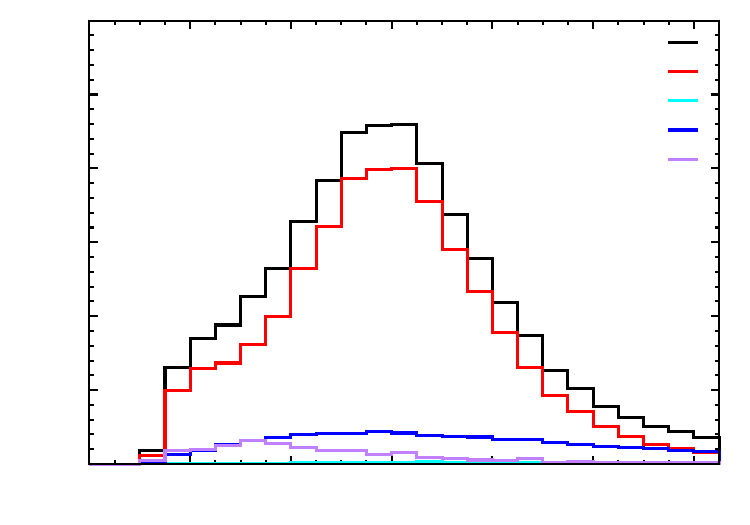
\includegraphics{pics/hkdr_app_fhc}}%
    \gplfronttext
  \end{picture}%
\endgroup
}
	\resizebox{0.49\linewidth}{!}{% GNUPLOT: LaTeX picture with Postscript
\begingroup
  \makeatletter
  \providecommand\color[2][]{%
    \GenericError{(gnuplot) \space\space\space\@spaces}{%
      Package color not loaded in conjunction with
      terminal option `colourtext'%
    }{See the gnuplot documentation for explanation.%
    }{Either use 'blacktext' in gnuplot or load the package
      color.sty in LaTeX.}%
    \renewcommand\color[2][]{}%
  }%
  \providecommand\includegraphics[2][]{%
    \GenericError{(gnuplot) \space\space\space\@spaces}{%
      Package graphicx or graphics not loaded%
    }{See the gnuplot documentation for explanation.%
    }{The gnuplot epslatex terminal needs graphicx.sty or graphics.sty.}%
    \renewcommand\includegraphics[2][]{}%
  }%
  \providecommand\rotatebox[2]{#2}%
  \@ifundefined{ifGPcolor}{%
    \newif\ifGPcolor
    \GPcolortrue
  }{}%
  \@ifundefined{ifGPblacktext}{%
    \newif\ifGPblacktext
    \GPblacktexttrue
  }{}%
  % define a \g@addto@macro without @ in the name:
  \let\gplgaddtomacro\g@addto@macro
  % define empty templates for all commands taking text:
  \gdef\gplbacktext{}%
  \gdef\gplfronttext{}%
  \makeatother
  \ifGPblacktext
    % no textcolor at all
    \def\colorrgb#1{}%
    \def\colorgray#1{}%
  \else
    % gray or color?
    \ifGPcolor
      \def\colorrgb#1{\color[rgb]{#1}}%
      \def\colorgray#1{\color[gray]{#1}}%
      \expandafter\def\csname LTw\endcsname{\color{white}}%
      \expandafter\def\csname LTb\endcsname{\color{black}}%
      \expandafter\def\csname LTa\endcsname{\color{black}}%
      \expandafter\def\csname LT0\endcsname{\color[rgb]{1,0,0}}%
      \expandafter\def\csname LT1\endcsname{\color[rgb]{0,1,0}}%
      \expandafter\def\csname LT2\endcsname{\color[rgb]{0,0,1}}%
      \expandafter\def\csname LT3\endcsname{\color[rgb]{1,0,1}}%
      \expandafter\def\csname LT4\endcsname{\color[rgb]{0,1,1}}%
      \expandafter\def\csname LT5\endcsname{\color[rgb]{1,1,0}}%
      \expandafter\def\csname LT6\endcsname{\color[rgb]{0,0,0}}%
      \expandafter\def\csname LT7\endcsname{\color[rgb]{1,0.3,0}}%
      \expandafter\def\csname LT8\endcsname{\color[rgb]{0.5,0.5,0.5}}%
    \else
      % gray
      \def\colorrgb#1{\color{black}}%
      \def\colorgray#1{\color[gray]{#1}}%
      \expandafter\def\csname LTw\endcsname{\color{white}}%
      \expandafter\def\csname LTb\endcsname{\color{black}}%
      \expandafter\def\csname LTa\endcsname{\color{black}}%
      \expandafter\def\csname LT0\endcsname{\color{black}}%
      \expandafter\def\csname LT1\endcsname{\color{black}}%
      \expandafter\def\csname LT2\endcsname{\color{black}}%
      \expandafter\def\csname LT3\endcsname{\color{black}}%
      \expandafter\def\csname LT4\endcsname{\color{black}}%
      \expandafter\def\csname LT5\endcsname{\color{black}}%
      \expandafter\def\csname LT6\endcsname{\color{black}}%
      \expandafter\def\csname LT7\endcsname{\color{black}}%
      \expandafter\def\csname LT8\endcsname{\color{black}}%
    \fi
  \fi
    \setlength{\unitlength}{0.0500bp}%
    \ifx\gptboxheight\undefined%
      \newlength{\gptboxheight}%
      \newlength{\gptboxwidth}%
      \newsavebox{\gptboxtext}%
    \fi%
    \setlength{\fboxrule}{0.5pt}%
    \setlength{\fboxsep}{1pt}%
\begin{picture}(7200.00,5040.00)%
    \gplgaddtomacro\gplbacktext{%
      \csname LTb\endcsname%%
      \put(747,595){\makebox(0,0)[r]{\strut{}0}}%
      \csname LTb\endcsname%%
      \put(747,1305){\makebox(0,0)[r]{\strut{}1000}}%
      \csname LTb\endcsname%%
      \put(747,2014){\makebox(0,0)[r]{\strut{}2000}}%
      \csname LTb\endcsname%%
      \put(747,2724){\makebox(0,0)[r]{\strut{}3000}}%
      \csname LTb\endcsname%%
      \put(747,3434){\makebox(0,0)[r]{\strut{}4000}}%
      \csname LTb\endcsname%%
      \put(747,4143){\makebox(0,0)[r]{\strut{}5000}}%
      \csname LTb\endcsname%%
      \put(747,4853){\makebox(0,0)[r]{\strut{}6000}}%
      \csname LTb\endcsname%%
      \put(849,409){\makebox(0,0){\strut{}0}}%
      \csname LTb\endcsname%%
      \put(1816,409){\makebox(0,0){\strut{}0.2}}%
      \csname LTb\endcsname%%
      \put(2783,409){\makebox(0,0){\strut{}0.4}}%
      \csname LTb\endcsname%%
      \put(3750,409){\makebox(0,0){\strut{}0.6}}%
      \csname LTb\endcsname%%
      \put(4717,409){\makebox(0,0){\strut{}0.8}}%
      \csname LTb\endcsname%%
      \put(5684,409){\makebox(0,0){\strut{}1}}%
      \csname LTb\endcsname%%
      \put(6651,409){\makebox(0,0){\strut{}1.2}}%
      \csname LTb\endcsname%%
      \put(1151,4512){\makebox(0,0)[l]{\strut{}Design}}%
      \csname LTb\endcsname%%
      \put(1151,4214){\makebox(0,0)[l]{\strut{}$\cj{\nu}$-mode}}%
    }%
    \gplgaddtomacro\gplfronttext{%
      \csname LTb\endcsname%%
      \put(153,2724){\rotatebox{-270}{\makebox(0,0){\strut{}Events / GeV}}}%
      \csname LTb\endcsname%%
      \put(3871,130){\makebox(0,0){\strut{}Energy (GeV)}}%
      \csname LTb\endcsname%%
      \put(6309,4639){\makebox(0,0)[r]{\strut{}Total}}%
      \csname LTb\endcsname%%
      \put(6309,4360){\makebox(0,0)[r]{\strut{}$\nu_\mu \to \nu_e$}}%
      \csname LTb\endcsname%%
      \put(6309,4081){\makebox(0,0)[r]{\strut{}$\cj{\nu}_\mu \to \cj{\nu}_e$}}%
      \csname LTb\endcsname%%
      \put(6309,3802){\makebox(0,0)[r]{\strut{}$\nu_e + \cj{\nu}_e$}}%
      \csname LTb\endcsname%%
      \put(6309,3523){\makebox(0,0)[r]{\strut{}$\nu_\mu + \cj{\nu}_\mu$}}%
    }%
    \gplbacktext
    \put(0,0){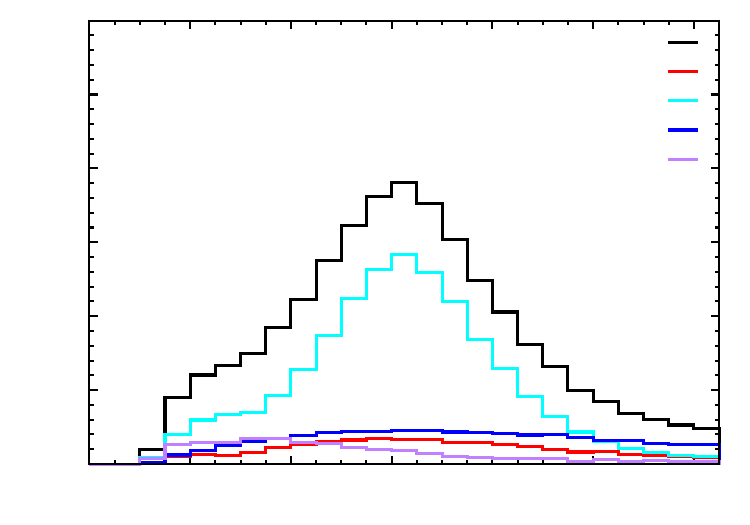
\includegraphics{pics/hkdr_app_rhc}}%
    \gplfronttext
  \end{picture}%
\endgroup
}
	\resizebox{0.49\linewidth}{!}{% GNUPLOT: LaTeX picture with Postscript
\begingroup
  \makeatletter
  \providecommand\color[2][]{%
    \GenericError{(gnuplot) \space\space\space\@spaces}{%
      Package color not loaded in conjunction with
      terminal option `colourtext'%
    }{See the gnuplot documentation for explanation.%
    }{Either use 'blacktext' in gnuplot or load the package
      color.sty in LaTeX.}%
    \renewcommand\color[2][]{}%
  }%
  \providecommand\includegraphics[2][]{%
    \GenericError{(gnuplot) \space\space\space\@spaces}{%
      Package graphicx or graphics not loaded%
    }{See the gnuplot documentation for explanation.%
    }{The gnuplot epslatex terminal needs graphicx.sty or graphics.sty.}%
    \renewcommand\includegraphics[2][]{}%
  }%
  \providecommand\rotatebox[2]{#2}%
  \@ifundefined{ifGPcolor}{%
    \newif\ifGPcolor
    \GPcolortrue
  }{}%
  \@ifundefined{ifGPblacktext}{%
    \newif\ifGPblacktext
    \GPblacktexttrue
  }{}%
  % define a \g@addto@macro without @ in the name:
  \let\gplgaddtomacro\g@addto@macro
  % define empty templates for all commands taking text:
  \gdef\gplbacktext{}%
  \gdef\gplfronttext{}%
  \makeatother
  \ifGPblacktext
    % no textcolor at all
    \def\colorrgb#1{}%
    \def\colorgray#1{}%
  \else
    % gray or color?
    \ifGPcolor
      \def\colorrgb#1{\color[rgb]{#1}}%
      \def\colorgray#1{\color[gray]{#1}}%
      \expandafter\def\csname LTw\endcsname{\color{white}}%
      \expandafter\def\csname LTb\endcsname{\color{black}}%
      \expandafter\def\csname LTa\endcsname{\color{black}}%
      \expandafter\def\csname LT0\endcsname{\color[rgb]{1,0,0}}%
      \expandafter\def\csname LT1\endcsname{\color[rgb]{0,1,0}}%
      \expandafter\def\csname LT2\endcsname{\color[rgb]{0,0,1}}%
      \expandafter\def\csname LT3\endcsname{\color[rgb]{1,0,1}}%
      \expandafter\def\csname LT4\endcsname{\color[rgb]{0,1,1}}%
      \expandafter\def\csname LT5\endcsname{\color[rgb]{1,1,0}}%
      \expandafter\def\csname LT6\endcsname{\color[rgb]{0,0,0}}%
      \expandafter\def\csname LT7\endcsname{\color[rgb]{1,0.3,0}}%
      \expandafter\def\csname LT8\endcsname{\color[rgb]{0.5,0.5,0.5}}%
    \else
      % gray
      \def\colorrgb#1{\color{black}}%
      \def\colorgray#1{\color[gray]{#1}}%
      \expandafter\def\csname LTw\endcsname{\color{white}}%
      \expandafter\def\csname LTb\endcsname{\color{black}}%
      \expandafter\def\csname LTa\endcsname{\color{black}}%
      \expandafter\def\csname LT0\endcsname{\color{black}}%
      \expandafter\def\csname LT1\endcsname{\color{black}}%
      \expandafter\def\csname LT2\endcsname{\color{black}}%
      \expandafter\def\csname LT3\endcsname{\color{black}}%
      \expandafter\def\csname LT4\endcsname{\color{black}}%
      \expandafter\def\csname LT5\endcsname{\color{black}}%
      \expandafter\def\csname LT6\endcsname{\color{black}}%
      \expandafter\def\csname LT7\endcsname{\color{black}}%
      \expandafter\def\csname LT8\endcsname{\color{black}}%
    \fi
  \fi
    \setlength{\unitlength}{0.0500bp}%
    \ifx\gptboxheight\undefined%
      \newlength{\gptboxheight}%
      \newlength{\gptboxwidth}%
      \newsavebox{\gptboxtext}%
    \fi%
    \setlength{\fboxrule}{0.5pt}%
    \setlength{\fboxsep}{1pt}%
\begin{picture}(7200.00,5040.00)%
    \gplgaddtomacro\gplbacktext{%
      \csname LTb\endcsname%%
      \put(645,595){\makebox(0,0)[r]{\strut{}0}}%
      \csname LTb\endcsname%%
      \put(645,1305){\makebox(0,0)[r]{\strut{}50}}%
      \csname LTb\endcsname%%
      \put(645,2014){\makebox(0,0)[r]{\strut{}100}}%
      \csname LTb\endcsname%%
      \put(645,2724){\makebox(0,0)[r]{\strut{}150}}%
      \csname LTb\endcsname%%
      \put(645,3434){\makebox(0,0)[r]{\strut{}200}}%
      \csname LTb\endcsname%%
      \put(645,4143){\makebox(0,0)[r]{\strut{}250}}%
      \csname LTb\endcsname%%
      \put(645,4853){\makebox(0,0)[r]{\strut{}300}}%
      \csname LTb\endcsname%%
      \put(747,409){\makebox(0,0){\strut{}0}}%
      \csname LTb\endcsname%%
      \put(1730,409){\makebox(0,0){\strut{}0.2}}%
      \csname LTb\endcsname%%
      \put(2714,409){\makebox(0,0){\strut{}0.4}}%
      \csname LTb\endcsname%%
      \put(3697,409){\makebox(0,0){\strut{}0.6}}%
      \csname LTb\endcsname%%
      \put(4680,409){\makebox(0,0){\strut{}0.8}}%
      \csname LTb\endcsname%%
      \put(5664,409){\makebox(0,0){\strut{}1}}%
      \csname LTb\endcsname%%
      \put(6647,409){\makebox(0,0){\strut{}1.2}}%
    }%
    \gplgaddtomacro\gplfronttext{%
      \csname LTb\endcsname%%
      \put(153,2724){\rotatebox{-270}{\makebox(0,0){\strut{}Number of events}}}%
      \csname LTb\endcsname%%
      \put(3820,130){\makebox(0,0){\strut{}Energy (GeV)}}%
      \csname LTb\endcsname%%
      \put(6309,4639){\makebox(0,0)[r]{\strut{}Total}}%
      \csname LTb\endcsname%%
      \put(6309,4360){\makebox(0,0)[r]{\strut{}$\nu_\mu \to \nu_e$}}%
      \csname LTb\endcsname%%
      \put(6309,4081){\makebox(0,0)[r]{\strut{}$\cj{\nu}_\mu \to \cj{\nu}_e$}}%
      \csname LTb\endcsname%%
      \put(6309,3802){\makebox(0,0)[r]{\strut{}$\nu_e + \cj{\nu}_e$}}%
      \csname LTb\endcsname%%
      \put(6309,3523){\makebox(0,0)[r]{\strut{}$\nu_\mu + \cj{\nu}_\mu$}}%
    }%
    \gplbacktext
    \put(0,0){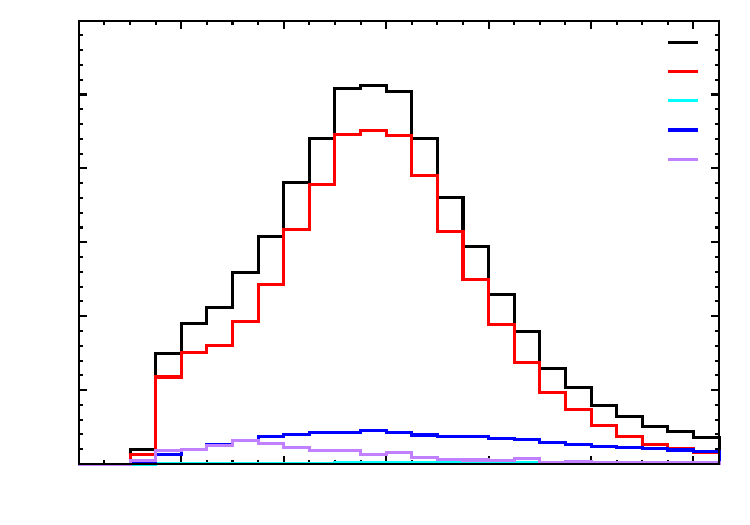
\includegraphics{pics/asim_app_fhc}}%
    \gplfronttext
  \end{picture}%
\endgroup
}
	\resizebox{0.49\linewidth}{!}{% GNUPLOT: LaTeX picture with Postscript
\begingroup
  \makeatletter
  \providecommand\color[2][]{%
    \GenericError{(gnuplot) \space\space\space\@spaces}{%
      Package color not loaded in conjunction with
      terminal option `colourtext'%
    }{See the gnuplot documentation for explanation.%
    }{Either use 'blacktext' in gnuplot or load the package
      color.sty in LaTeX.}%
    \renewcommand\color[2][]{}%
  }%
  \providecommand\includegraphics[2][]{%
    \GenericError{(gnuplot) \space\space\space\@spaces}{%
      Package graphicx or graphics not loaded%
    }{See the gnuplot documentation for explanation.%
    }{The gnuplot epslatex terminal needs graphicx.sty or graphics.sty.}%
    \renewcommand\includegraphics[2][]{}%
  }%
  \providecommand\rotatebox[2]{#2}%
  \@ifundefined{ifGPcolor}{%
    \newif\ifGPcolor
    \GPcolortrue
  }{}%
  \@ifundefined{ifGPblacktext}{%
    \newif\ifGPblacktext
    \GPblacktexttrue
  }{}%
  % define a \g@addto@macro without @ in the name:
  \let\gplgaddtomacro\g@addto@macro
  % define empty templates for all commands taking text:
  \gdef\gplbacktext{}%
  \gdef\gplfronttext{}%
  \makeatother
  \ifGPblacktext
    % no textcolor at all
    \def\colorrgb#1{}%
    \def\colorgray#1{}%
  \else
    % gray or color?
    \ifGPcolor
      \def\colorrgb#1{\color[rgb]{#1}}%
      \def\colorgray#1{\color[gray]{#1}}%
      \expandafter\def\csname LTw\endcsname{\color{white}}%
      \expandafter\def\csname LTb\endcsname{\color{black}}%
      \expandafter\def\csname LTa\endcsname{\color{black}}%
      \expandafter\def\csname LT0\endcsname{\color[rgb]{1,0,0}}%
      \expandafter\def\csname LT1\endcsname{\color[rgb]{0,1,0}}%
      \expandafter\def\csname LT2\endcsname{\color[rgb]{0,0,1}}%
      \expandafter\def\csname LT3\endcsname{\color[rgb]{1,0,1}}%
      \expandafter\def\csname LT4\endcsname{\color[rgb]{0,1,1}}%
      \expandafter\def\csname LT5\endcsname{\color[rgb]{1,1,0}}%
      \expandafter\def\csname LT6\endcsname{\color[rgb]{0,0,0}}%
      \expandafter\def\csname LT7\endcsname{\color[rgb]{1,0.3,0}}%
      \expandafter\def\csname LT8\endcsname{\color[rgb]{0.5,0.5,0.5}}%
    \else
      % gray
      \def\colorrgb#1{\color{black}}%
      \def\colorgray#1{\color[gray]{#1}}%
      \expandafter\def\csname LTw\endcsname{\color{white}}%
      \expandafter\def\csname LTb\endcsname{\color{black}}%
      \expandafter\def\csname LTa\endcsname{\color{black}}%
      \expandafter\def\csname LT0\endcsname{\color{black}}%
      \expandafter\def\csname LT1\endcsname{\color{black}}%
      \expandafter\def\csname LT2\endcsname{\color{black}}%
      \expandafter\def\csname LT3\endcsname{\color{black}}%
      \expandafter\def\csname LT4\endcsname{\color{black}}%
      \expandafter\def\csname LT5\endcsname{\color{black}}%
      \expandafter\def\csname LT6\endcsname{\color{black}}%
      \expandafter\def\csname LT7\endcsname{\color{black}}%
      \expandafter\def\csname LT8\endcsname{\color{black}}%
    \fi
  \fi
    \setlength{\unitlength}{0.0500bp}%
    \ifx\gptboxheight\undefined%
      \newlength{\gptboxheight}%
      \newlength{\gptboxwidth}%
      \newsavebox{\gptboxtext}%
    \fi%
    \setlength{\fboxrule}{0.5pt}%
    \setlength{\fboxsep}{1pt}%
\begin{picture}(7200.00,5040.00)%
    \gplgaddtomacro\gplbacktext{%
      \csname LTb\endcsname%%
      \put(747,595){\makebox(0,0)[r]{\strut{}0}}%
      \csname LTb\endcsname%%
      \put(747,1305){\makebox(0,0)[r]{\strut{}1000}}%
      \csname LTb\endcsname%%
      \put(747,2014){\makebox(0,0)[r]{\strut{}2000}}%
      \csname LTb\endcsname%%
      \put(747,2724){\makebox(0,0)[r]{\strut{}3000}}%
      \csname LTb\endcsname%%
      \put(747,3434){\makebox(0,0)[r]{\strut{}4000}}%
      \csname LTb\endcsname%%
      \put(747,4143){\makebox(0,0)[r]{\strut{}5000}}%
      \csname LTb\endcsname%%
      \put(747,4853){\makebox(0,0)[r]{\strut{}6000}}%
      \csname LTb\endcsname%%
      \put(849,409){\makebox(0,0){\strut{}0}}%
      \csname LTb\endcsname%%
      \put(1816,409){\makebox(0,0){\strut{}0.2}}%
      \csname LTb\endcsname%%
      \put(2783,409){\makebox(0,0){\strut{}0.4}}%
      \csname LTb\endcsname%%
      \put(3750,409){\makebox(0,0){\strut{}0.6}}%
      \csname LTb\endcsname%%
      \put(4717,409){\makebox(0,0){\strut{}0.8}}%
      \csname LTb\endcsname%%
      \put(5684,409){\makebox(0,0){\strut{}1}}%
      \csname LTb\endcsname%%
      \put(6651,409){\makebox(0,0){\strut{}1.2}}%
      \csname LTb\endcsname%%
      \put(1151,4512){\makebox(0,0)[l]{\strut{}Asimov A}}%
      \csname LTb\endcsname%%
      \put(1151,4214){\makebox(0,0)[l]{\strut{}$\cj{\nu}$-mode}}%
    }%
    \gplgaddtomacro\gplfronttext{%
      \csname LTb\endcsname%%
      \put(153,2724){\rotatebox{-270}{\makebox(0,0){\strut{}Events / GeV}}}%
      \csname LTb\endcsname%%
      \put(3871,130){\makebox(0,0){\strut{}Energy (GeV)}}%
      \csname LTb\endcsname%%
      \put(6309,4639){\makebox(0,0)[r]{\strut{}Total}}%
      \csname LTb\endcsname%%
      \put(6309,4360){\makebox(0,0)[r]{\strut{}$\nu_\mu \to \nu_e$}}%
      \csname LTb\endcsname%%
      \put(6309,4081){\makebox(0,0)[r]{\strut{}$\cj{\nu}_\mu \to \cj{\nu}_e$}}%
      \csname LTb\endcsname%%
      \put(6309,3802){\makebox(0,0)[r]{\strut{}$\nu_e + \cj{\nu}_e$}}%
      \csname LTb\endcsname%%
      \put(6309,3523){\makebox(0,0)[r]{\strut{}$\nu_\mu + \cj{\nu}_\mu$}}%
    }%
    \gplbacktext
    \put(0,0){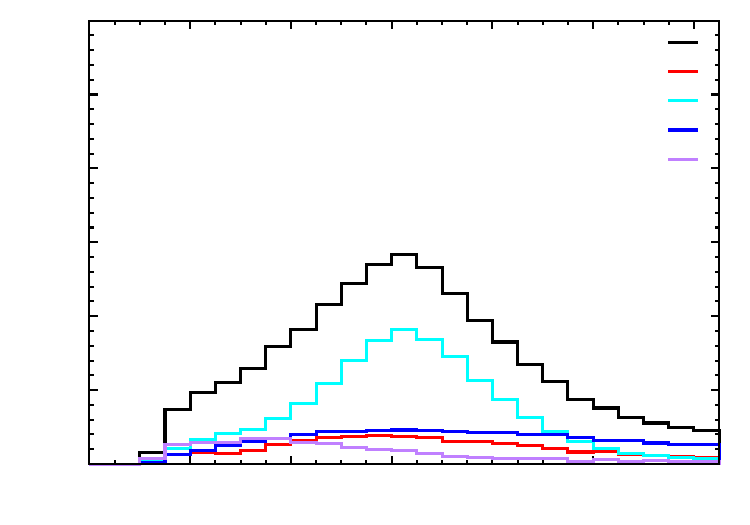
\includegraphics{pics/asim_app_rhc}}%
    \gplfronttext
  \end{picture}%
\endgroup
}
	\caption[Predicted distribution of one ring $e$-like events]%
		{The predicted distribution of one ring $e$-like events with respect to reconstructed energy at HK %
		are shown here for $\nu$-mode (left) and $\cj{\nu}$-mode.
		The appearance signals $\nu_\mu \to \nu_e$ and $\cj{\nu}_\mu \to \cj{\nu}_e$ are compared to the %
		background events.
		The spectra on the top and bottom panel are generated using respectively %
		the Design Report and the Asimov~A oscillation parameters (see \reftab{tab:asimovA}).}
	\label{fig:reco_spectra_e}
\end{figure}

\begin{figure}[t]
	\centering
	\resizebox{0.49\linewidth}{!}{% GNUPLOT: LaTeX picture with Postscript
\begingroup
  \makeatletter
  \providecommand\color[2][]{%
    \GenericError{(gnuplot) \space\space\space\@spaces}{%
      Package color not loaded in conjunction with
      terminal option `colourtext'%
    }{See the gnuplot documentation for explanation.%
    }{Either use 'blacktext' in gnuplot or load the package
      color.sty in LaTeX.}%
    \renewcommand\color[2][]{}%
  }%
  \providecommand\includegraphics[2][]{%
    \GenericError{(gnuplot) \space\space\space\@spaces}{%
      Package graphicx or graphics not loaded%
    }{See the gnuplot documentation for explanation.%
    }{The gnuplot epslatex terminal needs graphicx.sty or graphics.sty.}%
    \renewcommand\includegraphics[2][]{}%
  }%
  \providecommand\rotatebox[2]{#2}%
  \@ifundefined{ifGPcolor}{%
    \newif\ifGPcolor
    \GPcolortrue
  }{}%
  \@ifundefined{ifGPblacktext}{%
    \newif\ifGPblacktext
    \GPblacktexttrue
  }{}%
  % define a \g@addto@macro without @ in the name:
  \let\gplgaddtomacro\g@addto@macro
  % define empty templates for all commands taking text:
  \gdef\gplbacktext{}%
  \gdef\gplfronttext{}%
  \makeatother
  \ifGPblacktext
    % no textcolor at all
    \def\colorrgb#1{}%
    \def\colorgray#1{}%
  \else
    % gray or color?
    \ifGPcolor
      \def\colorrgb#1{\color[rgb]{#1}}%
      \def\colorgray#1{\color[gray]{#1}}%
      \expandafter\def\csname LTw\endcsname{\color{white}}%
      \expandafter\def\csname LTb\endcsname{\color{black}}%
      \expandafter\def\csname LTa\endcsname{\color{black}}%
      \expandafter\def\csname LT0\endcsname{\color[rgb]{1,0,0}}%
      \expandafter\def\csname LT1\endcsname{\color[rgb]{0,1,0}}%
      \expandafter\def\csname LT2\endcsname{\color[rgb]{0,0,1}}%
      \expandafter\def\csname LT3\endcsname{\color[rgb]{1,0,1}}%
      \expandafter\def\csname LT4\endcsname{\color[rgb]{0,1,1}}%
      \expandafter\def\csname LT5\endcsname{\color[rgb]{1,1,0}}%
      \expandafter\def\csname LT6\endcsname{\color[rgb]{0,0,0}}%
      \expandafter\def\csname LT7\endcsname{\color[rgb]{1,0.3,0}}%
      \expandafter\def\csname LT8\endcsname{\color[rgb]{0.5,0.5,0.5}}%
    \else
      % gray
      \def\colorrgb#1{\color{black}}%
      \def\colorgray#1{\color[gray]{#1}}%
      \expandafter\def\csname LTw\endcsname{\color{white}}%
      \expandafter\def\csname LTb\endcsname{\color{black}}%
      \expandafter\def\csname LTa\endcsname{\color{black}}%
      \expandafter\def\csname LT0\endcsname{\color{black}}%
      \expandafter\def\csname LT1\endcsname{\color{black}}%
      \expandafter\def\csname LT2\endcsname{\color{black}}%
      \expandafter\def\csname LT3\endcsname{\color{black}}%
      \expandafter\def\csname LT4\endcsname{\color{black}}%
      \expandafter\def\csname LT5\endcsname{\color{black}}%
      \expandafter\def\csname LT6\endcsname{\color{black}}%
      \expandafter\def\csname LT7\endcsname{\color{black}}%
      \expandafter\def\csname LT8\endcsname{\color{black}}%
    \fi
  \fi
    \setlength{\unitlength}{0.0500bp}%
    \ifx\gptboxheight\undefined%
      \newlength{\gptboxheight}%
      \newlength{\gptboxwidth}%
      \newsavebox{\gptboxtext}%
    \fi%
    \setlength{\fboxrule}{0.5pt}%
    \setlength{\fboxsep}{1pt}%
\begin{picture}(7200.00,5040.00)%
    \gplgaddtomacro\gplbacktext{%
      \csname LTb\endcsname%%
      \put(645,595){\makebox(0,0)[r]{\strut{}0}}%
      \csname LTb\endcsname%%
      \put(645,1203){\makebox(0,0)[r]{\strut{}100}}%
      \csname LTb\endcsname%%
      \put(645,1812){\makebox(0,0)[r]{\strut{}200}}%
      \csname LTb\endcsname%%
      \put(645,2420){\makebox(0,0)[r]{\strut{}300}}%
      \csname LTb\endcsname%%
      \put(645,3028){\makebox(0,0)[r]{\strut{}400}}%
      \csname LTb\endcsname%%
      \put(645,3636){\makebox(0,0)[r]{\strut{}500}}%
      \csname LTb\endcsname%%
      \put(645,4245){\makebox(0,0)[r]{\strut{}600}}%
      \csname LTb\endcsname%%
      \put(645,4853){\makebox(0,0)[r]{\strut{}700}}%
      \csname LTb\endcsname%%
      \put(747,409){\makebox(0,0){\strut{}0}}%
      \csname LTb\endcsname%%
      \put(1976,409){\makebox(0,0){\strut{}1}}%
      \csname LTb\endcsname%%
      \put(3205,409){\makebox(0,0){\strut{}2}}%
      \csname LTb\endcsname%%
      \put(4435,409){\makebox(0,0){\strut{}3}}%
      \csname LTb\endcsname%%
      \put(5664,409){\makebox(0,0){\strut{}4}}%
      \csname LTb\endcsname%%
      \put(6893,409){\makebox(0,0){\strut{}5}}%
    }%
    \gplgaddtomacro\gplfronttext{%
      \csname LTb\endcsname%%
      \put(153,2724){\rotatebox{-270}{\makebox(0,0){\strut{}Number of events}}}%
      \csname LTb\endcsname%%
      \put(3820,130){\makebox(0,0){\strut{}Energy (GeV)}}%
      \csname LTb\endcsname%%
      \put(6309,4639){\makebox(0,0)[r]{\strut{}Total}}%
      \csname LTb\endcsname%%
      \put(6309,4360){\makebox(0,0)[r]{\strut{}$\nu_\mu \to \nu_\mu$}}%
      \csname LTb\endcsname%%
      \put(6309,4081){\makebox(0,0)[r]{\strut{}$\cj{\nu}_\mu \to \cj{\nu}_\mu$}}%
      \csname LTb\endcsname%%
      \put(6309,3802){\makebox(0,0)[r]{\strut{}$\nu_e + \cj{\nu}_e$}}%
    }%
    \gplbacktext
    \put(0,0){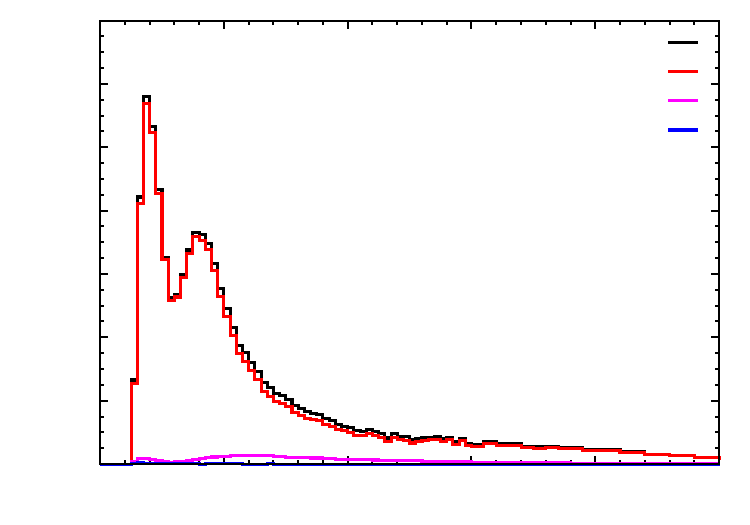
\includegraphics{pics/hkdr_dis_fhc}}%
    \gplfronttext
  \end{picture}%
\endgroup
}
	\resizebox{0.49\linewidth}{!}{% GNUPLOT: LaTeX picture with Postscript
\begingroup
  \makeatletter
  \providecommand\color[2][]{%
    \GenericError{(gnuplot) \space\space\space\@spaces}{%
      Package color not loaded in conjunction with
      terminal option `colourtext'%
    }{See the gnuplot documentation for explanation.%
    }{Either use 'blacktext' in gnuplot or load the package
      color.sty in LaTeX.}%
    \renewcommand\color[2][]{}%
  }%
  \providecommand\includegraphics[2][]{%
    \GenericError{(gnuplot) \space\space\space\@spaces}{%
      Package graphicx or graphics not loaded%
    }{See the gnuplot documentation for explanation.%
    }{The gnuplot epslatex terminal needs graphicx.sty or graphics.sty.}%
    \renewcommand\includegraphics[2][]{}%
  }%
  \providecommand\rotatebox[2]{#2}%
  \@ifundefined{ifGPcolor}{%
    \newif\ifGPcolor
    \GPcolortrue
  }{}%
  \@ifundefined{ifGPblacktext}{%
    \newif\ifGPblacktext
    \GPblacktexttrue
  }{}%
  % define a \g@addto@macro without @ in the name:
  \let\gplgaddtomacro\g@addto@macro
  % define empty templates for all commands taking text:
  \gdef\gplbacktext{}%
  \gdef\gplfronttext{}%
  \makeatother
  \ifGPblacktext
    % no textcolor at all
    \def\colorrgb#1{}%
    \def\colorgray#1{}%
  \else
    % gray or color?
    \ifGPcolor
      \def\colorrgb#1{\color[rgb]{#1}}%
      \def\colorgray#1{\color[gray]{#1}}%
      \expandafter\def\csname LTw\endcsname{\color{white}}%
      \expandafter\def\csname LTb\endcsname{\color{black}}%
      \expandafter\def\csname LTa\endcsname{\color{black}}%
      \expandafter\def\csname LT0\endcsname{\color[rgb]{1,0,0}}%
      \expandafter\def\csname LT1\endcsname{\color[rgb]{0,1,0}}%
      \expandafter\def\csname LT2\endcsname{\color[rgb]{0,0,1}}%
      \expandafter\def\csname LT3\endcsname{\color[rgb]{1,0,1}}%
      \expandafter\def\csname LT4\endcsname{\color[rgb]{0,1,1}}%
      \expandafter\def\csname LT5\endcsname{\color[rgb]{1,1,0}}%
      \expandafter\def\csname LT6\endcsname{\color[rgb]{0,0,0}}%
      \expandafter\def\csname LT7\endcsname{\color[rgb]{1,0.3,0}}%
      \expandafter\def\csname LT8\endcsname{\color[rgb]{0.5,0.5,0.5}}%
    \else
      % gray
      \def\colorrgb#1{\color{black}}%
      \def\colorgray#1{\color[gray]{#1}}%
      \expandafter\def\csname LTw\endcsname{\color{white}}%
      \expandafter\def\csname LTb\endcsname{\color{black}}%
      \expandafter\def\csname LTa\endcsname{\color{black}}%
      \expandafter\def\csname LT0\endcsname{\color{black}}%
      \expandafter\def\csname LT1\endcsname{\color{black}}%
      \expandafter\def\csname LT2\endcsname{\color{black}}%
      \expandafter\def\csname LT3\endcsname{\color{black}}%
      \expandafter\def\csname LT4\endcsname{\color{black}}%
      \expandafter\def\csname LT5\endcsname{\color{black}}%
      \expandafter\def\csname LT6\endcsname{\color{black}}%
      \expandafter\def\csname LT7\endcsname{\color{black}}%
      \expandafter\def\csname LT8\endcsname{\color{black}}%
    \fi
  \fi
    \setlength{\unitlength}{0.0500bp}%
    \ifx\gptboxheight\undefined%
      \newlength{\gptboxheight}%
      \newlength{\gptboxwidth}%
      \newsavebox{\gptboxtext}%
    \fi%
    \setlength{\fboxrule}{0.5pt}%
    \setlength{\fboxsep}{1pt}%
\begin{picture}(7200.00,5040.00)%
    \gplgaddtomacro\gplbacktext{%
      \csname LTb\endcsname%%
      \put(849,595){\makebox(0,0)[r]{\strut{}0}}%
      \csname LTb\endcsname%%
      \put(849,1203){\makebox(0,0)[r]{\strut{}2000}}%
      \csname LTb\endcsname%%
      \put(849,1812){\makebox(0,0)[r]{\strut{}4000}}%
      \csname LTb\endcsname%%
      \put(849,2420){\makebox(0,0)[r]{\strut{}6000}}%
      \csname LTb\endcsname%%
      \put(849,3028){\makebox(0,0)[r]{\strut{}8000}}%
      \csname LTb\endcsname%%
      \put(849,3636){\makebox(0,0)[r]{\strut{}10000}}%
      \csname LTb\endcsname%%
      \put(849,4245){\makebox(0,0)[r]{\strut{}12000}}%
      \csname LTb\endcsname%%
      \put(849,4853){\makebox(0,0)[r]{\strut{}14000}}%
      \csname LTb\endcsname%%
      \put(951,409){\makebox(0,0){\strut{}0}}%
      \csname LTb\endcsname%%
      \put(2139,409){\makebox(0,0){\strut{}1}}%
      \csname LTb\endcsname%%
      \put(3328,409){\makebox(0,0){\strut{}2}}%
      \csname LTb\endcsname%%
      \put(4516,409){\makebox(0,0){\strut{}3}}%
      \csname LTb\endcsname%%
      \put(5705,409){\makebox(0,0){\strut{}4}}%
      \csname LTb\endcsname%%
      \put(6893,409){\makebox(0,0){\strut{}5}}%
      \csname LTb\endcsname%%
      \put(3328,4512){\makebox(0,0)[l]{\strut{}Design}}%
      \csname LTb\endcsname%%
      \put(3328,4214){\makebox(0,0)[l]{\strut{}$\cj{\nu}$-mode}}%
    }%
    \gplgaddtomacro\gplfronttext{%
      \csname LTb\endcsname%%
      \put(153,2724){\rotatebox{-270}{\makebox(0,0){\strut{}Events / GeV}}}%
      \csname LTb\endcsname%%
      \put(3922,130){\makebox(0,0){\strut{}Energy (GeV)}}%
      \csname LTb\endcsname%%
      \put(6309,4639){\makebox(0,0)[r]{\strut{}Total}}%
      \csname LTb\endcsname%%
      \put(6309,4360){\makebox(0,0)[r]{\strut{}$\nu_\mu \to \nu_\mu$}}%
      \csname LTb\endcsname%%
      \put(6309,4081){\makebox(0,0)[r]{\strut{}$\cj{\nu}_\mu \to \cj{\nu}_\mu$}}%
      \csname LTb\endcsname%%
      \put(6309,3802){\makebox(0,0)[r]{\strut{}$\nu_e + \cj{\nu}_e$}}%
    }%
    \gplbacktext
    \put(0,0){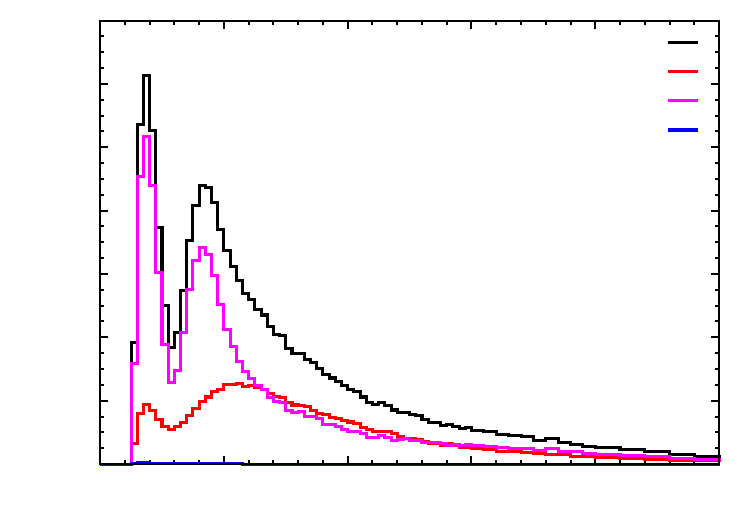
\includegraphics{pics/hkdr_dis_rhc}}%
    \gplfronttext
  \end{picture}%
\endgroup
}
	\resizebox{0.49\linewidth}{!}{% GNUPLOT: LaTeX picture with Postscript
\begingroup
  \makeatletter
  \providecommand\color[2][]{%
    \GenericError{(gnuplot) \space\space\space\@spaces}{%
      Package color not loaded in conjunction with
      terminal option `colourtext'%
    }{See the gnuplot documentation for explanation.%
    }{Either use 'blacktext' in gnuplot or load the package
      color.sty in LaTeX.}%
    \renewcommand\color[2][]{}%
  }%
  \providecommand\includegraphics[2][]{%
    \GenericError{(gnuplot) \space\space\space\@spaces}{%
      Package graphicx or graphics not loaded%
    }{See the gnuplot documentation for explanation.%
    }{The gnuplot epslatex terminal needs graphicx.sty or graphics.sty.}%
    \renewcommand\includegraphics[2][]{}%
  }%
  \providecommand\rotatebox[2]{#2}%
  \@ifundefined{ifGPcolor}{%
    \newif\ifGPcolor
    \GPcolortrue
  }{}%
  \@ifundefined{ifGPblacktext}{%
    \newif\ifGPblacktext
    \GPblacktexttrue
  }{}%
  % define a \g@addto@macro without @ in the name:
  \let\gplgaddtomacro\g@addto@macro
  % define empty templates for all commands taking text:
  \gdef\gplbacktext{}%
  \gdef\gplfronttext{}%
  \makeatother
  \ifGPblacktext
    % no textcolor at all
    \def\colorrgb#1{}%
    \def\colorgray#1{}%
  \else
    % gray or color?
    \ifGPcolor
      \def\colorrgb#1{\color[rgb]{#1}}%
      \def\colorgray#1{\color[gray]{#1}}%
      \expandafter\def\csname LTw\endcsname{\color{white}}%
      \expandafter\def\csname LTb\endcsname{\color{black}}%
      \expandafter\def\csname LTa\endcsname{\color{black}}%
      \expandafter\def\csname LT0\endcsname{\color[rgb]{1,0,0}}%
      \expandafter\def\csname LT1\endcsname{\color[rgb]{0,1,0}}%
      \expandafter\def\csname LT2\endcsname{\color[rgb]{0,0,1}}%
      \expandafter\def\csname LT3\endcsname{\color[rgb]{1,0,1}}%
      \expandafter\def\csname LT4\endcsname{\color[rgb]{0,1,1}}%
      \expandafter\def\csname LT5\endcsname{\color[rgb]{1,1,0}}%
      \expandafter\def\csname LT6\endcsname{\color[rgb]{0,0,0}}%
      \expandafter\def\csname LT7\endcsname{\color[rgb]{1,0.3,0}}%
      \expandafter\def\csname LT8\endcsname{\color[rgb]{0.5,0.5,0.5}}%
    \else
      % gray
      \def\colorrgb#1{\color{black}}%
      \def\colorgray#1{\color[gray]{#1}}%
      \expandafter\def\csname LTw\endcsname{\color{white}}%
      \expandafter\def\csname LTb\endcsname{\color{black}}%
      \expandafter\def\csname LTa\endcsname{\color{black}}%
      \expandafter\def\csname LT0\endcsname{\color{black}}%
      \expandafter\def\csname LT1\endcsname{\color{black}}%
      \expandafter\def\csname LT2\endcsname{\color{black}}%
      \expandafter\def\csname LT3\endcsname{\color{black}}%
      \expandafter\def\csname LT4\endcsname{\color{black}}%
      \expandafter\def\csname LT5\endcsname{\color{black}}%
      \expandafter\def\csname LT6\endcsname{\color{black}}%
      \expandafter\def\csname LT7\endcsname{\color{black}}%
      \expandafter\def\csname LT8\endcsname{\color{black}}%
    \fi
  \fi
    \setlength{\unitlength}{0.0500bp}%
    \ifx\gptboxheight\undefined%
      \newlength{\gptboxheight}%
      \newlength{\gptboxwidth}%
      \newsavebox{\gptboxtext}%
    \fi%
    \setlength{\fboxrule}{0.5pt}%
    \setlength{\fboxsep}{1pt}%
\begin{picture}(7200.00,5040.00)%
    \gplgaddtomacro\gplbacktext{%
      \csname LTb\endcsname%%
      \put(645,595){\makebox(0,0)[r]{\strut{}0}}%
      \csname LTb\endcsname%%
      \put(645,1203){\makebox(0,0)[r]{\strut{}100}}%
      \csname LTb\endcsname%%
      \put(645,1812){\makebox(0,0)[r]{\strut{}200}}%
      \csname LTb\endcsname%%
      \put(645,2420){\makebox(0,0)[r]{\strut{}300}}%
      \csname LTb\endcsname%%
      \put(645,3028){\makebox(0,0)[r]{\strut{}400}}%
      \csname LTb\endcsname%%
      \put(645,3636){\makebox(0,0)[r]{\strut{}500}}%
      \csname LTb\endcsname%%
      \put(645,4245){\makebox(0,0)[r]{\strut{}600}}%
      \csname LTb\endcsname%%
      \put(645,4853){\makebox(0,0)[r]{\strut{}700}}%
      \csname LTb\endcsname%%
      \put(747,409){\makebox(0,0){\strut{}0}}%
      \csname LTb\endcsname%%
      \put(1976,409){\makebox(0,0){\strut{}1}}%
      \csname LTb\endcsname%%
      \put(3205,409){\makebox(0,0){\strut{}2}}%
      \csname LTb\endcsname%%
      \put(4435,409){\makebox(0,0){\strut{}3}}%
      \csname LTb\endcsname%%
      \put(5664,409){\makebox(0,0){\strut{}4}}%
      \csname LTb\endcsname%%
      \put(6893,409){\makebox(0,0){\strut{}5}}%
    }%
    \gplgaddtomacro\gplfronttext{%
      \csname LTb\endcsname%%
      \put(153,2724){\rotatebox{-270}{\makebox(0,0){\strut{}Number of events}}}%
      \csname LTb\endcsname%%
      \put(3820,130){\makebox(0,0){\strut{}Energy (GeV)}}%
      \csname LTb\endcsname%%
      \put(6309,4639){\makebox(0,0)[r]{\strut{}Total}}%
      \csname LTb\endcsname%%
      \put(6309,4360){\makebox(0,0)[r]{\strut{}$\nu_\mu \to \nu_\mu$}}%
      \csname LTb\endcsname%%
      \put(6309,4081){\makebox(0,0)[r]{\strut{}$\cj{\nu}_\mu \to \cj{\nu}_\mu$}}%
      \csname LTb\endcsname%%
      \put(6309,3802){\makebox(0,0)[r]{\strut{}$\nu_e + \cj{\nu}_e$}}%
    }%
    \gplbacktext
    \put(0,0){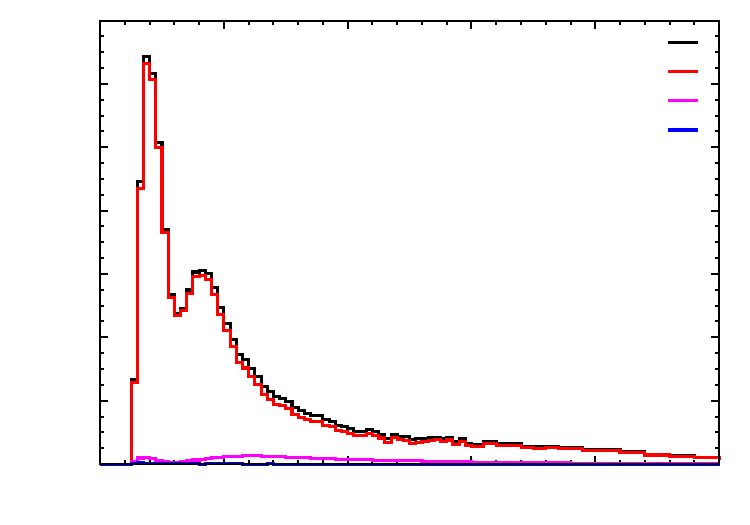
\includegraphics{pics/asim_dis_fhc}}%
    \gplfronttext
  \end{picture}%
\endgroup
}
	\resizebox{0.49\linewidth}{!}{% GNUPLOT: LaTeX picture with Postscript
\begingroup
  \makeatletter
  \providecommand\color[2][]{%
    \GenericError{(gnuplot) \space\space\space\@spaces}{%
      Package color not loaded in conjunction with
      terminal option `colourtext'%
    }{See the gnuplot documentation for explanation.%
    }{Either use 'blacktext' in gnuplot or load the package
      color.sty in LaTeX.}%
    \renewcommand\color[2][]{}%
  }%
  \providecommand\includegraphics[2][]{%
    \GenericError{(gnuplot) \space\space\space\@spaces}{%
      Package graphicx or graphics not loaded%
    }{See the gnuplot documentation for explanation.%
    }{The gnuplot epslatex terminal needs graphicx.sty or graphics.sty.}%
    \renewcommand\includegraphics[2][]{}%
  }%
  \providecommand\rotatebox[2]{#2}%
  \@ifundefined{ifGPcolor}{%
    \newif\ifGPcolor
    \GPcolortrue
  }{}%
  \@ifundefined{ifGPblacktext}{%
    \newif\ifGPblacktext
    \GPblacktexttrue
  }{}%
  % define a \g@addto@macro without @ in the name:
  \let\gplgaddtomacro\g@addto@macro
  % define empty templates for all commands taking text:
  \gdef\gplbacktext{}%
  \gdef\gplfronttext{}%
  \makeatother
  \ifGPblacktext
    % no textcolor at all
    \def\colorrgb#1{}%
    \def\colorgray#1{}%
  \else
    % gray or color?
    \ifGPcolor
      \def\colorrgb#1{\color[rgb]{#1}}%
      \def\colorgray#1{\color[gray]{#1}}%
      \expandafter\def\csname LTw\endcsname{\color{white}}%
      \expandafter\def\csname LTb\endcsname{\color{black}}%
      \expandafter\def\csname LTa\endcsname{\color{black}}%
      \expandafter\def\csname LT0\endcsname{\color[rgb]{1,0,0}}%
      \expandafter\def\csname LT1\endcsname{\color[rgb]{0,1,0}}%
      \expandafter\def\csname LT2\endcsname{\color[rgb]{0,0,1}}%
      \expandafter\def\csname LT3\endcsname{\color[rgb]{1,0,1}}%
      \expandafter\def\csname LT4\endcsname{\color[rgb]{0,1,1}}%
      \expandafter\def\csname LT5\endcsname{\color[rgb]{1,1,0}}%
      \expandafter\def\csname LT6\endcsname{\color[rgb]{0,0,0}}%
      \expandafter\def\csname LT7\endcsname{\color[rgb]{1,0.3,0}}%
      \expandafter\def\csname LT8\endcsname{\color[rgb]{0.5,0.5,0.5}}%
    \else
      % gray
      \def\colorrgb#1{\color{black}}%
      \def\colorgray#1{\color[gray]{#1}}%
      \expandafter\def\csname LTw\endcsname{\color{white}}%
      \expandafter\def\csname LTb\endcsname{\color{black}}%
      \expandafter\def\csname LTa\endcsname{\color{black}}%
      \expandafter\def\csname LT0\endcsname{\color{black}}%
      \expandafter\def\csname LT1\endcsname{\color{black}}%
      \expandafter\def\csname LT2\endcsname{\color{black}}%
      \expandafter\def\csname LT3\endcsname{\color{black}}%
      \expandafter\def\csname LT4\endcsname{\color{black}}%
      \expandafter\def\csname LT5\endcsname{\color{black}}%
      \expandafter\def\csname LT6\endcsname{\color{black}}%
      \expandafter\def\csname LT7\endcsname{\color{black}}%
      \expandafter\def\csname LT8\endcsname{\color{black}}%
    \fi
  \fi
    \setlength{\unitlength}{0.0500bp}%
    \ifx\gptboxheight\undefined%
      \newlength{\gptboxheight}%
      \newlength{\gptboxwidth}%
      \newsavebox{\gptboxtext}%
    \fi%
    \setlength{\fboxrule}{0.5pt}%
    \setlength{\fboxsep}{1pt}%
\begin{picture}(7200.00,5040.00)%
    \gplgaddtomacro\gplbacktext{%
      \csname LTb\endcsname%%
      \put(645,595){\makebox(0,0)[r]{\strut{}0}}%
      \csname LTb\endcsname%%
      \put(645,1203){\makebox(0,0)[r]{\strut{}100}}%
      \csname LTb\endcsname%%
      \put(645,1812){\makebox(0,0)[r]{\strut{}200}}%
      \csname LTb\endcsname%%
      \put(645,2420){\makebox(0,0)[r]{\strut{}300}}%
      \csname LTb\endcsname%%
      \put(645,3028){\makebox(0,0)[r]{\strut{}400}}%
      \csname LTb\endcsname%%
      \put(645,3636){\makebox(0,0)[r]{\strut{}500}}%
      \csname LTb\endcsname%%
      \put(645,4245){\makebox(0,0)[r]{\strut{}600}}%
      \csname LTb\endcsname%%
      \put(645,4853){\makebox(0,0)[r]{\strut{}700}}%
      \csname LTb\endcsname%%
      \put(747,409){\makebox(0,0){\strut{}0}}%
      \csname LTb\endcsname%%
      \put(1976,409){\makebox(0,0){\strut{}1}}%
      \csname LTb\endcsname%%
      \put(3205,409){\makebox(0,0){\strut{}2}}%
      \csname LTb\endcsname%%
      \put(4435,409){\makebox(0,0){\strut{}3}}%
      \csname LTb\endcsname%%
      \put(5664,409){\makebox(0,0){\strut{}4}}%
      \csname LTb\endcsname%%
      \put(6893,409){\makebox(0,0){\strut{}5}}%
    }%
    \gplgaddtomacro\gplfronttext{%
      \csname LTb\endcsname%%
      \put(153,2724){\rotatebox{-270}{\makebox(0,0){\strut{}Number of events}}}%
      \csname LTb\endcsname%%
      \put(3820,130){\makebox(0,0){\strut{}Energy (GeV)}}%
      \csname LTb\endcsname%%
      \put(6309,4639){\makebox(0,0)[r]{\strut{}Total}}%
      \csname LTb\endcsname%%
      \put(6309,4360){\makebox(0,0)[r]{\strut{}$\nu_\mu \to \nu_\mu$}}%
      \csname LTb\endcsname%%
      \put(6309,4081){\makebox(0,0)[r]{\strut{}$\cj{\nu}_\mu \to \cj{\nu}_\mu$}}%
      \csname LTb\endcsname%%
      \put(6309,3802){\makebox(0,0)[r]{\strut{}$\nu_e + \cj{\nu}_e$}}%
    }%
    \gplbacktext
    \put(0,0){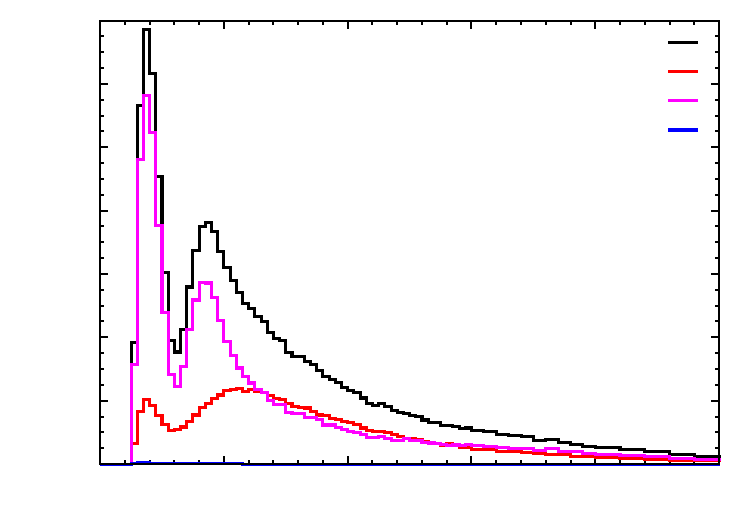
\includegraphics{pics/asim_dis_rhc}}%
    \gplfronttext
  \end{picture}%
\endgroup
}
	\caption[Predicted distribution of one ring $\mu$-like events]%
		{The predicted distribution of one ring $\mu$-like events with respect to reconstructed energy at HK %
		are shown here for $\nu$-mode (left) and $\cj{\nu}$-mode.
		The disappearance events $\nu_\mu \to \nu_\mu$ and $\cj{\nu}_\mu \to \cj{\nu}_\mu$ %
		are compared to the small contributions from electron neutrinos.
		The spectra on the top and bottom panel are generated using respectively %
		the Design Report and the Asimov~A oscillation parameters (see \reftab{tab:asimovA}).}
	\label{fig:reco_spectra_mu}
\end{figure}

The simulation of the HK detector heavily relies on the techniques established by the SK and T2K collaborations.
Neutrinos interactions are generated using NEUT~\cite{Hayato:2002sd}, also employed in SK and T2K.
The response of the detector is simulated using the SK-IV full Monte Carlo simulation, which uses the GEANT3~\cite{Brun:1994aa}.
Events are reconstructed with the SK reconstruction software, which gives a realistic estimate of the HK performance.
The criteria to select neutrino candidates in MC simulations follows a similar prescription to the one used in SK.
Only fully contained events within the inner detector are considered, provided that the reconstructed vertex %
is more than 1.5\,m away from the ID walls (fiducial volume) and that the collected charge from the PMTs, $E_\text{vis}$, %
amounts to an energy greater than 30\,MeV.
The purity of the data sample is controlled by requiring the detection of a single Cherenkov ring.
In this way, the chance of selecting only CCQE events is enhanced.
The neutrino energy is reconstructed from the energy of the final state charged lepton and %
the angle between the neutrino beam and the charged lepton direction, applying \refeq{eq:e_reco}.
Electron-flavour events are selected by requiring an $e$-like ring, deposited energy %
in the range $100\,\text{MeV} < E_\text{vis} < 1.25\,\text{GeV}$, %
and no decay electron associated to the event, typical of a muon decay.
The muon sample is built by requiring a $\mu$-like ring, a reconstructed muon momentum greater than $200$\,MeV %
and the presence of the electron from the Michel decay of the muon.
The simulation is run assuming an integrated beam power of 13\,MW, corresponding to \np{2.7e22}\,POT %
collected over 10 years with a 30\,GeV proton beam.
The proportion between the amount of data collected in neutrino and antineutrino modes is set to $\nu : \cj{\nu} = 1:3$.
The ratio is chosen in order to have similar number of events in $\nu$- and $\cj{\nu}$-mode samples.
The reconstructed spectra from the simulations are shown in \reffigs{fig:reco_spectra_e}{fig:reco_spectra_mu} %
where two different oscillation parameter combinations are compared to illustrate the effect of neutrino oscillation;
the contributions from different oscillation channels to the overall distributions are also highlighted.



\subsection{Validation of the fitter}
\label{sec:nuenorm}

Before employing the full systematic model, the fitting framework is validated with %
a special systematic set for the beam sample.
It is composed of just two systematics: the $\nu_e$ and the $\cj{\nu}_e$ CC cross-section uncertainties.
These two errors are implemented twice, either as correlated or as anticorrelated, %
and they are tested at different values (1\%, 2\%, 3\%, 4\%, and 5\%) for a total of ten combinations.
The correlation matrices used are simply
\begin{equation}
	\rho = \mqty(\hphantom{-}1 & \hphantom{-}1 \\ \hphantom{-}1 & \hphantom{-}1) \quad\text{and}\quad
	\rho = \mqty(\hphantom{-}1 & -1 \\ -1 & \hphantom{-}1) \ ,
\end{equation}
but they are both singular and not invertible.
A small offset of \np{e-5} is added to off-diagonal terms to allow the calculation of the $\chi^2$.
Due to the definition of the $\chi^2$ in \refeq{eq:chi2}, %
the difference between fits with the same relative error lies in the correlation matrix, %
whereas at fixed correlation the effect of the systematics on the likelihood is given by the $1\sigma$ histograms.

\begin{figure}
	\centering
	\resizebox{0.49\linewidth}{!}{% GNUPLOT: LaTeX picture with Postscript
\begingroup
  \makeatletter
  \providecommand\color[2][]{%
    \GenericError{(gnuplot) \space\space\space\@spaces}{%
      Package color not loaded in conjunction with
      terminal option `colourtext'%
    }{See the gnuplot documentation for explanation.%
    }{Either use 'blacktext' in gnuplot or load the package
      color.sty in LaTeX.}%
    \renewcommand\color[2][]{}%
  }%
  \providecommand\includegraphics[2][]{%
    \GenericError{(gnuplot) \space\space\space\@spaces}{%
      Package graphicx or graphics not loaded%
    }{See the gnuplot documentation for explanation.%
    }{The gnuplot epslatex terminal needs graphicx.sty or graphics.sty.}%
    \renewcommand\includegraphics[2][]{}%
  }%
  \providecommand\rotatebox[2]{#2}%
  \@ifundefined{ifGPcolor}{%
    \newif\ifGPcolor
    \GPcolortrue
  }{}%
  \@ifundefined{ifGPblacktext}{%
    \newif\ifGPblacktext
    \GPblacktexttrue
  }{}%
  % define a \g@addto@macro without @ in the name:
  \let\gplgaddtomacro\g@addto@macro
  % define empty templates for all commands taking text:
  \gdef\gplbacktext{}%
  \gdef\gplfronttext{}%
  \makeatother
  \ifGPblacktext
    % no textcolor at all
    \def\colorrgb#1{}%
    \def\colorgray#1{}%
  \else
    % gray or color?
    \ifGPcolor
      \def\colorrgb#1{\color[rgb]{#1}}%
      \def\colorgray#1{\color[gray]{#1}}%
      \expandafter\def\csname LTw\endcsname{\color{white}}%
      \expandafter\def\csname LTb\endcsname{\color{black}}%
      \expandafter\def\csname LTa\endcsname{\color{black}}%
      \expandafter\def\csname LT0\endcsname{\color[rgb]{1,0,0}}%
      \expandafter\def\csname LT1\endcsname{\color[rgb]{0,1,0}}%
      \expandafter\def\csname LT2\endcsname{\color[rgb]{0,0,1}}%
      \expandafter\def\csname LT3\endcsname{\color[rgb]{1,0,1}}%
      \expandafter\def\csname LT4\endcsname{\color[rgb]{0,1,1}}%
      \expandafter\def\csname LT5\endcsname{\color[rgb]{1,1,0}}%
      \expandafter\def\csname LT6\endcsname{\color[rgb]{0,0,0}}%
      \expandafter\def\csname LT7\endcsname{\color[rgb]{1,0.3,0}}%
      \expandafter\def\csname LT8\endcsname{\color[rgb]{0.5,0.5,0.5}}%
    \else
      % gray
      \def\colorrgb#1{\color{black}}%
      \def\colorgray#1{\color[gray]{#1}}%
      \expandafter\def\csname LTw\endcsname{\color{white}}%
      \expandafter\def\csname LTb\endcsname{\color{black}}%
      \expandafter\def\csname LTa\endcsname{\color{black}}%
      \expandafter\def\csname LT0\endcsname{\color{black}}%
      \expandafter\def\csname LT1\endcsname{\color{black}}%
      \expandafter\def\csname LT2\endcsname{\color{black}}%
      \expandafter\def\csname LT3\endcsname{\color{black}}%
      \expandafter\def\csname LT4\endcsname{\color{black}}%
      \expandafter\def\csname LT5\endcsname{\color{black}}%
      \expandafter\def\csname LT6\endcsname{\color{black}}%
      \expandafter\def\csname LT7\endcsname{\color{black}}%
      \expandafter\def\csname LT8\endcsname{\color{black}}%
    \fi
  \fi
    \setlength{\unitlength}{0.0500bp}%
    \ifx\gptboxheight\undefined%
      \newlength{\gptboxheight}%
      \newlength{\gptboxwidth}%
      \newsavebox{\gptboxtext}%
    \fi%
    \setlength{\fboxrule}{0.5pt}%
    \setlength{\fboxsep}{1pt}%
\begin{picture}(7200.00,3600.00)%
    \gplgaddtomacro\gplbacktext{%
      \csname LTb\endcsname%%
      \put(618,720){\makebox(0,0)[r]{\strut{}1}}%
      \csname LTb\endcsname%%
      \put(618,1080){\makebox(0,0)[r]{\strut{}1.02}}%
      \csname LTb\endcsname%%
      \put(618,1440){\makebox(0,0)[r]{\strut{}1.04}}%
      \csname LTb\endcsname%%
      \put(720,354){\makebox(0,0){\strut{}0}}%
      \csname LTb\endcsname%%
      \put(1363,354){\makebox(0,0){\strut{}0.125}}%
      \csname LTb\endcsname%%
      \put(2006,354){\makebox(0,0){\strut{}0.25}}%
      \csname LTb\endcsname%%
      \put(2648,354){\makebox(0,0){\strut{}0.375}}%
      \csname LTb\endcsname%%
      \put(3291,354){\makebox(0,0){\strut{}0.5}}%
      \csname LTb\endcsname%%
      \put(3934,354){\makebox(0,0){\strut{}0.625}}%
      \csname LTb\endcsname%%
      \put(4577,354){\makebox(0,0){\strut{}0.75}}%
      \csname LTb\endcsname%%
      \put(5220,354){\makebox(0,0){\strut{}0.875}}%
      \csname LTb\endcsname%%
      \put(5862,354){\makebox(0,0){\strut{}1}}%
      \csname LTb\endcsname%%
      \put(6505,354){\makebox(0,0){\strut{}1.125}}%
      \csname LTb\endcsname%%
      \put(7148,354){\makebox(0,0){\strut{}1.25}}%
    }%
    \gplgaddtomacro\gplfronttext{%
      \csname LTb\endcsname%%
      \put(24,1170){\rotatebox{-270}{\makebox(0,0){\strut{}$1\sigma$ histogram}}}%
      \csname LTb\endcsname%%
      \put(3934,75){\makebox(0,0){\strut{}Energy (GeV)}}%
    }%
    \gplgaddtomacro\gplbacktext{%
      \csname LTb\endcsname%%
      \put(618,1800){\makebox(0,0)[r]{\strut{}0}}%
      \csname LTb\endcsname%%
      \put(618,2141){\makebox(0,0)[r]{\strut{}50}}%
      \csname LTb\endcsname%%
      \put(618,2482){\makebox(0,0)[r]{\strut{}100}}%
      \csname LTb\endcsname%%
      \put(618,2824){\makebox(0,0)[r]{\strut{}150}}%
      \csname LTb\endcsname%%
      \put(618,3165){\makebox(0,0)[r]{\strut{}200}}%
      \csname LTb\endcsname%%
      \put(618,3506){\makebox(0,0)[r]{\strut{}250}}%
      \csname LTb\endcsname%%
      \put(720,1614){\makebox(0,0){\strut{}}}%
      \csname LTb\endcsname%%
      \put(1363,1614){\makebox(0,0){\strut{}}}%
      \csname LTb\endcsname%%
      \put(2006,1614){\makebox(0,0){\strut{}}}%
      \csname LTb\endcsname%%
      \put(2648,1614){\makebox(0,0){\strut{}}}%
      \csname LTb\endcsname%%
      \put(3291,1614){\makebox(0,0){\strut{}}}%
      \csname LTb\endcsname%%
      \put(3934,1614){\makebox(0,0){\strut{}}}%
      \csname LTb\endcsname%%
      \put(4577,1614){\makebox(0,0){\strut{}}}%
      \csname LTb\endcsname%%
      \put(5220,1614){\makebox(0,0){\strut{}}}%
      \csname LTb\endcsname%%
      \put(5862,1614){\makebox(0,0){\strut{}}}%
      \csname LTb\endcsname%%
      \put(6505,1614){\makebox(0,0){\strut{}}}%
      \csname LTb\endcsname%%
      \put(7148,1614){\makebox(0,0){\strut{}}}%
    }%
    \gplgaddtomacro\gplfronttext{%
      \csname LTb\endcsname%%
      \put(126,2653){\rotatebox{-270}{\makebox(0,0){\strut{}Events}}}%
      \csname LTb\endcsname%%
      \put(3934,1558){\makebox(0,0){\strut{}}}%
      \csname LTb\endcsname%%
      \put(6009,2409){\makebox(0,0)[l]{\strut{}No syst}}%
      \csname LTb\endcsname%%
      \put(6309,2595){\makebox(0,0)[l]{\strut{}1\%}}%
      \csname LTb\endcsname%%
      \put(6309,2781){\makebox(0,0)[l]{\strut{}2\%}}%
      \csname LTb\endcsname%%
      \put(6309,2967){\makebox(0,0)[l]{\strut{}3\%}}%
      \csname LTb\endcsname%%
      \put(6309,3153){\makebox(0,0)[l]{\strut{}4\%}}%
      \csname LTb\endcsname%%
      \put(6309,3339){\makebox(0,0)[l]{\strut{}5\%}}%
    }%
    \gplbacktext
    \put(0,0){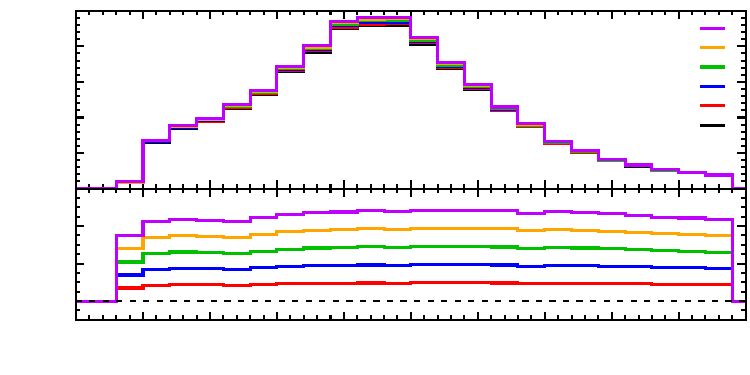
\includegraphics{nuenorm_E_FHC_sys0}}%
    \gplfronttext
  \end{picture}%
\endgroup
}
	\hfill
	\resizebox{0.49\linewidth}{!}{% GNUPLOT: LaTeX picture with Postscript
\begingroup
  \makeatletter
  \providecommand\color[2][]{%
    \GenericError{(gnuplot) \space\space\space\@spaces}{%
      Package color not loaded in conjunction with
      terminal option `colourtext'%
    }{See the gnuplot documentation for explanation.%
    }{Either use 'blacktext' in gnuplot or load the package
      color.sty in LaTeX.}%
    \renewcommand\color[2][]{}%
  }%
  \providecommand\includegraphics[2][]{%
    \GenericError{(gnuplot) \space\space\space\@spaces}{%
      Package graphicx or graphics not loaded%
    }{See the gnuplot documentation for explanation.%
    }{The gnuplot epslatex terminal needs graphicx.sty or graphics.sty.}%
    \renewcommand\includegraphics[2][]{}%
  }%
  \providecommand\rotatebox[2]{#2}%
  \@ifundefined{ifGPcolor}{%
    \newif\ifGPcolor
    \GPcolortrue
  }{}%
  \@ifundefined{ifGPblacktext}{%
    \newif\ifGPblacktext
    \GPblacktexttrue
  }{}%
  % define a \g@addto@macro without @ in the name:
  \let\gplgaddtomacro\g@addto@macro
  % define empty templates for all commands taking text:
  \gdef\gplbacktext{}%
  \gdef\gplfronttext{}%
  \makeatother
  \ifGPblacktext
    % no textcolor at all
    \def\colorrgb#1{}%
    \def\colorgray#1{}%
  \else
    % gray or color?
    \ifGPcolor
      \def\colorrgb#1{\color[rgb]{#1}}%
      \def\colorgray#1{\color[gray]{#1}}%
      \expandafter\def\csname LTw\endcsname{\color{white}}%
      \expandafter\def\csname LTb\endcsname{\color{black}}%
      \expandafter\def\csname LTa\endcsname{\color{black}}%
      \expandafter\def\csname LT0\endcsname{\color[rgb]{1,0,0}}%
      \expandafter\def\csname LT1\endcsname{\color[rgb]{0,1,0}}%
      \expandafter\def\csname LT2\endcsname{\color[rgb]{0,0,1}}%
      \expandafter\def\csname LT3\endcsname{\color[rgb]{1,0,1}}%
      \expandafter\def\csname LT4\endcsname{\color[rgb]{0,1,1}}%
      \expandafter\def\csname LT5\endcsname{\color[rgb]{1,1,0}}%
      \expandafter\def\csname LT6\endcsname{\color[rgb]{0,0,0}}%
      \expandafter\def\csname LT7\endcsname{\color[rgb]{1,0.3,0}}%
      \expandafter\def\csname LT8\endcsname{\color[rgb]{0.5,0.5,0.5}}%
    \else
      % gray
      \def\colorrgb#1{\color{black}}%
      \def\colorgray#1{\color[gray]{#1}}%
      \expandafter\def\csname LTw\endcsname{\color{white}}%
      \expandafter\def\csname LTb\endcsname{\color{black}}%
      \expandafter\def\csname LTa\endcsname{\color{black}}%
      \expandafter\def\csname LT0\endcsname{\color{black}}%
      \expandafter\def\csname LT1\endcsname{\color{black}}%
      \expandafter\def\csname LT2\endcsname{\color{black}}%
      \expandafter\def\csname LT3\endcsname{\color{black}}%
      \expandafter\def\csname LT4\endcsname{\color{black}}%
      \expandafter\def\csname LT5\endcsname{\color{black}}%
      \expandafter\def\csname LT6\endcsname{\color{black}}%
      \expandafter\def\csname LT7\endcsname{\color{black}}%
      \expandafter\def\csname LT8\endcsname{\color{black}}%
    \fi
  \fi
    \setlength{\unitlength}{0.0500bp}%
    \ifx\gptboxheight\undefined%
      \newlength{\gptboxheight}%
      \newlength{\gptboxwidth}%
      \newsavebox{\gptboxtext}%
    \fi%
    \setlength{\fboxrule}{0.5pt}%
    \setlength{\fboxsep}{1pt}%
\begin{picture}(7200.00,3600.00)%
    \gplgaddtomacro\gplbacktext{%
      \csname LTb\endcsname%%
      \put(618,540){\makebox(0,0)[r]{\strut{}0.99}}%
      \csname LTb\endcsname%%
      \put(618,855){\makebox(0,0)[r]{\strut{}1}}%
      \csname LTb\endcsname%%
      \put(618,1170){\makebox(0,0)[r]{\strut{}1.01}}%
      \csname LTb\endcsname%%
      \put(618,1485){\makebox(0,0)[r]{\strut{}1.02}}%
      \csname LTb\endcsname%%
      \put(720,354){\makebox(0,0){\strut{}0}}%
      \csname LTb\endcsname%%
      \put(1363,354){\makebox(0,0){\strut{}0.125}}%
      \csname LTb\endcsname%%
      \put(2006,354){\makebox(0,0){\strut{}0.25}}%
      \csname LTb\endcsname%%
      \put(2648,354){\makebox(0,0){\strut{}0.375}}%
      \csname LTb\endcsname%%
      \put(3291,354){\makebox(0,0){\strut{}0.5}}%
      \csname LTb\endcsname%%
      \put(3934,354){\makebox(0,0){\strut{}0.625}}%
      \csname LTb\endcsname%%
      \put(4577,354){\makebox(0,0){\strut{}0.75}}%
      \csname LTb\endcsname%%
      \put(5220,354){\makebox(0,0){\strut{}0.875}}%
      \csname LTb\endcsname%%
      \put(5862,354){\makebox(0,0){\strut{}1}}%
      \csname LTb\endcsname%%
      \put(6505,354){\makebox(0,0){\strut{}1.125}}%
      \csname LTb\endcsname%%
      \put(7148,354){\makebox(0,0){\strut{}1.25}}%
    }%
    \gplgaddtomacro\gplfronttext{%
      \csname LTb\endcsname%%
      \put(24,1170){\rotatebox{-270}{\makebox(0,0){\strut{}$1\sigma$ histogram}}}%
      \csname LTb\endcsname%%
      \put(3934,75){\makebox(0,0){\strut{}Energy (GeV)}}%
    }%
    \gplgaddtomacro\gplbacktext{%
      \csname LTb\endcsname%%
      \put(618,1800){\makebox(0,0)[r]{\strut{}0}}%
      \csname LTb\endcsname%%
      \put(618,2227){\makebox(0,0)[r]{\strut{}50}}%
      \csname LTb\endcsname%%
      \put(618,2653){\makebox(0,0)[r]{\strut{}100}}%
      \csname LTb\endcsname%%
      \put(618,3080){\makebox(0,0)[r]{\strut{}150}}%
      \csname LTb\endcsname%%
      \put(618,3506){\makebox(0,0)[r]{\strut{}200}}%
      \csname LTb\endcsname%%
      \put(720,1614){\makebox(0,0){\strut{}}}%
      \csname LTb\endcsname%%
      \put(1363,1614){\makebox(0,0){\strut{}}}%
      \csname LTb\endcsname%%
      \put(2006,1614){\makebox(0,0){\strut{}}}%
      \csname LTb\endcsname%%
      \put(2648,1614){\makebox(0,0){\strut{}}}%
      \csname LTb\endcsname%%
      \put(3291,1614){\makebox(0,0){\strut{}}}%
      \csname LTb\endcsname%%
      \put(3934,1614){\makebox(0,0){\strut{}}}%
      \csname LTb\endcsname%%
      \put(4577,1614){\makebox(0,0){\strut{}}}%
      \csname LTb\endcsname%%
      \put(5220,1614){\makebox(0,0){\strut{}}}%
      \csname LTb\endcsname%%
      \put(5862,1614){\makebox(0,0){\strut{}}}%
      \csname LTb\endcsname%%
      \put(6505,1614){\makebox(0,0){\strut{}}}%
      \csname LTb\endcsname%%
      \put(7148,1614){\makebox(0,0){\strut{}}}%
    }%
    \gplgaddtomacro\gplfronttext{%
      \csname LTb\endcsname%%
      \put(126,2653){\rotatebox{-270}{\makebox(0,0){\strut{}Events}}}%
      \csname LTb\endcsname%%
      \put(3934,1558){\makebox(0,0){\strut{}}}%
      \csname LTb\endcsname%%
      \put(6009,2409){\makebox(0,0)[l]{\strut{}No syst}}%
      \csname LTb\endcsname%%
      \put(6309,2595){\makebox(0,0)[l]{\strut{}1\%}}%
      \csname LTb\endcsname%%
      \put(6309,2781){\makebox(0,0)[l]{\strut{}2\%}}%
      \csname LTb\endcsname%%
      \put(6309,2967){\makebox(0,0)[l]{\strut{}3\%}}%
      \csname LTb\endcsname%%
      \put(6309,3153){\makebox(0,0)[l]{\strut{}4\%}}%
      \csname LTb\endcsname%%
      \put(6309,3339){\makebox(0,0)[l]{\strut{}5\%}}%
    }%
    \gplbacktext
    \put(0,0){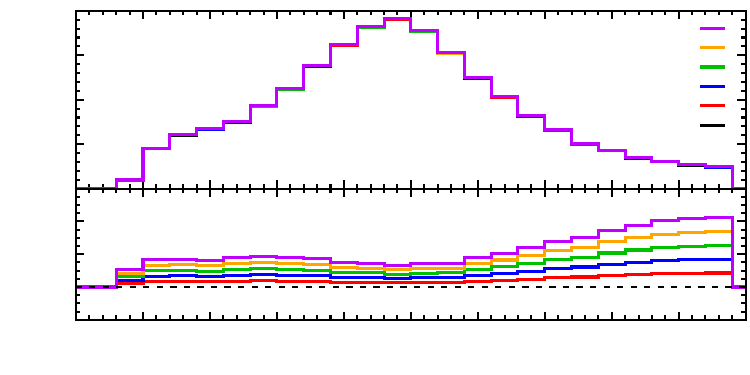
\includegraphics{nuenorm_E_RHC_sys0}}%
    \gplfronttext
  \end{picture}%
\endgroup
}

	\medskip
	\resizebox{0.49\linewidth}{!}{% GNUPLOT: LaTeX picture with Postscript
\begingroup
  \makeatletter
  \providecommand\color[2][]{%
    \GenericError{(gnuplot) \space\space\space\@spaces}{%
      Package color not loaded in conjunction with
      terminal option `colourtext'%
    }{See the gnuplot documentation for explanation.%
    }{Either use 'blacktext' in gnuplot or load the package
      color.sty in LaTeX.}%
    \renewcommand\color[2][]{}%
  }%
  \providecommand\includegraphics[2][]{%
    \GenericError{(gnuplot) \space\space\space\@spaces}{%
      Package graphicx or graphics not loaded%
    }{See the gnuplot documentation for explanation.%
    }{The gnuplot epslatex terminal needs graphicx.sty or graphics.sty.}%
    \renewcommand\includegraphics[2][]{}%
  }%
  \providecommand\rotatebox[2]{#2}%
  \@ifundefined{ifGPcolor}{%
    \newif\ifGPcolor
    \GPcolortrue
  }{}%
  \@ifundefined{ifGPblacktext}{%
    \newif\ifGPblacktext
    \GPblacktexttrue
  }{}%
  % define a \g@addto@macro without @ in the name:
  \let\gplgaddtomacro\g@addto@macro
  % define empty templates for all commands taking text:
  \gdef\gplbacktext{}%
  \gdef\gplfronttext{}%
  \makeatother
  \ifGPblacktext
    % no textcolor at all
    \def\colorrgb#1{}%
    \def\colorgray#1{}%
  \else
    % gray or color?
    \ifGPcolor
      \def\colorrgb#1{\color[rgb]{#1}}%
      \def\colorgray#1{\color[gray]{#1}}%
      \expandafter\def\csname LTw\endcsname{\color{white}}%
      \expandafter\def\csname LTb\endcsname{\color{black}}%
      \expandafter\def\csname LTa\endcsname{\color{black}}%
      \expandafter\def\csname LT0\endcsname{\color[rgb]{1,0,0}}%
      \expandafter\def\csname LT1\endcsname{\color[rgb]{0,1,0}}%
      \expandafter\def\csname LT2\endcsname{\color[rgb]{0,0,1}}%
      \expandafter\def\csname LT3\endcsname{\color[rgb]{1,0,1}}%
      \expandafter\def\csname LT4\endcsname{\color[rgb]{0,1,1}}%
      \expandafter\def\csname LT5\endcsname{\color[rgb]{1,1,0}}%
      \expandafter\def\csname LT6\endcsname{\color[rgb]{0,0,0}}%
      \expandafter\def\csname LT7\endcsname{\color[rgb]{1,0.3,0}}%
      \expandafter\def\csname LT8\endcsname{\color[rgb]{0.5,0.5,0.5}}%
    \else
      % gray
      \def\colorrgb#1{\color{black}}%
      \def\colorgray#1{\color[gray]{#1}}%
      \expandafter\def\csname LTw\endcsname{\color{white}}%
      \expandafter\def\csname LTb\endcsname{\color{black}}%
      \expandafter\def\csname LTa\endcsname{\color{black}}%
      \expandafter\def\csname LT0\endcsname{\color{black}}%
      \expandafter\def\csname LT1\endcsname{\color{black}}%
      \expandafter\def\csname LT2\endcsname{\color{black}}%
      \expandafter\def\csname LT3\endcsname{\color{black}}%
      \expandafter\def\csname LT4\endcsname{\color{black}}%
      \expandafter\def\csname LT5\endcsname{\color{black}}%
      \expandafter\def\csname LT6\endcsname{\color{black}}%
      \expandafter\def\csname LT7\endcsname{\color{black}}%
      \expandafter\def\csname LT8\endcsname{\color{black}}%
    \fi
  \fi
    \setlength{\unitlength}{0.0500bp}%
    \ifx\gptboxheight\undefined%
      \newlength{\gptboxheight}%
      \newlength{\gptboxwidth}%
      \newsavebox{\gptboxtext}%
    \fi%
    \setlength{\fboxrule}{0.5pt}%
    \setlength{\fboxsep}{1pt}%
\begin{picture}(7200.00,3600.00)%
    \gplgaddtomacro\gplbacktext{%
      \csname LTb\endcsname%%
      \put(618,792){\makebox(0,0)[r]{\strut{}1}}%
      \csname LTb\endcsname%%
      \put(618,1296){\makebox(0,0)[r]{\strut{}1.002}}%
      \csname LTb\endcsname%%
      \put(720,354){\makebox(0,0){\strut{}0}}%
      \csname LTb\endcsname%%
      \put(1363,354){\makebox(0,0){\strut{}0.125}}%
      \csname LTb\endcsname%%
      \put(2006,354){\makebox(0,0){\strut{}0.25}}%
      \csname LTb\endcsname%%
      \put(2648,354){\makebox(0,0){\strut{}0.375}}%
      \csname LTb\endcsname%%
      \put(3291,354){\makebox(0,0){\strut{}0.5}}%
      \csname LTb\endcsname%%
      \put(3934,354){\makebox(0,0){\strut{}0.625}}%
      \csname LTb\endcsname%%
      \put(4577,354){\makebox(0,0){\strut{}0.75}}%
      \csname LTb\endcsname%%
      \put(5220,354){\makebox(0,0){\strut{}0.875}}%
      \csname LTb\endcsname%%
      \put(5862,354){\makebox(0,0){\strut{}1}}%
      \csname LTb\endcsname%%
      \put(6505,354){\makebox(0,0){\strut{}1.125}}%
      \csname LTb\endcsname%%
      \put(7148,354){\makebox(0,0){\strut{}1.25}}%
    }%
    \gplgaddtomacro\gplfronttext{%
      \csname LTb\endcsname%%
      \put(3934,75){\makebox(0,0){\strut{}Energy (GeV)}}%
    }%
    \gplgaddtomacro\gplbacktext{%
      \csname LTb\endcsname%%
      \put(618,1800){\makebox(0,0)[r]{\strut{}0}}%
      \csname LTb\endcsname%%
      \put(618,2141){\makebox(0,0)[r]{\strut{}50}}%
      \csname LTb\endcsname%%
      \put(618,2482){\makebox(0,0)[r]{\strut{}100}}%
      \csname LTb\endcsname%%
      \put(618,2824){\makebox(0,0)[r]{\strut{}150}}%
      \csname LTb\endcsname%%
      \put(618,3165){\makebox(0,0)[r]{\strut{}200}}%
      \csname LTb\endcsname%%
      \put(618,3506){\makebox(0,0)[r]{\strut{}250}}%
      \csname LTb\endcsname%%
      \put(720,1614){\makebox(0,0){\strut{}}}%
      \csname LTb\endcsname%%
      \put(1363,1614){\makebox(0,0){\strut{}}}%
      \csname LTb\endcsname%%
      \put(2006,1614){\makebox(0,0){\strut{}}}%
      \csname LTb\endcsname%%
      \put(2648,1614){\makebox(0,0){\strut{}}}%
      \csname LTb\endcsname%%
      \put(3291,1614){\makebox(0,0){\strut{}}}%
      \csname LTb\endcsname%%
      \put(3934,1614){\makebox(0,0){\strut{}}}%
      \csname LTb\endcsname%%
      \put(4577,1614){\makebox(0,0){\strut{}}}%
      \csname LTb\endcsname%%
      \put(5220,1614){\makebox(0,0){\strut{}}}%
      \csname LTb\endcsname%%
      \put(5862,1614){\makebox(0,0){\strut{}}}%
      \csname LTb\endcsname%%
      \put(6505,1614){\makebox(0,0){\strut{}}}%
      \csname LTb\endcsname%%
      \put(7148,1614){\makebox(0,0){\strut{}}}%
    }%
    \gplgaddtomacro\gplfronttext{%
      \csname LTb\endcsname%%
      \put(126,2653){\rotatebox{-270}{\makebox(0,0){\strut{}Events}}}%
      \csname LTb\endcsname%%
      \put(3934,1558){\makebox(0,0){\strut{}}}%
      \csname LTb\endcsname%%
      \put(6009,2409){\makebox(0,0)[l]{\strut{}No syst}}%
      \csname LTb\endcsname%%
      \put(6309,2595){\makebox(0,0)[l]{\strut{}1\%}}%
      \csname LTb\endcsname%%
      \put(6309,2781){\makebox(0,0)[l]{\strut{}2\%}}%
      \csname LTb\endcsname%%
      \put(6309,2967){\makebox(0,0)[l]{\strut{}3\%}}%
      \csname LTb\endcsname%%
      \put(6309,3153){\makebox(0,0)[l]{\strut{}4\%}}%
      \csname LTb\endcsname%%
      \put(6309,3339){\makebox(0,0)[l]{\strut{}5\%}}%
    }%
    \gplbacktext
    \put(0,0){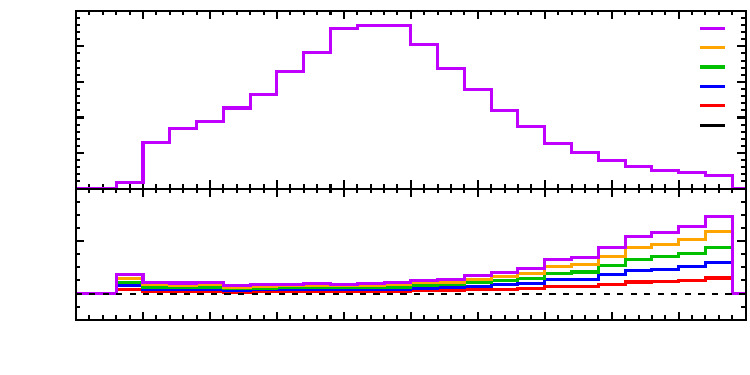
\includegraphics{nuenorm_E_FHC_sys1}}%
    \gplfronttext
  \end{picture}%
\endgroup
}
	\hfill
	\resizebox{0.49\linewidth}{!}{% GNUPLOT: LaTeX picture with Postscript
\begingroup
  \makeatletter
  \providecommand\color[2][]{%
    \GenericError{(gnuplot) \space\space\space\@spaces}{%
      Package color not loaded in conjunction with
      terminal option `colourtext'%
    }{See the gnuplot documentation for explanation.%
    }{Either use 'blacktext' in gnuplot or load the package
      color.sty in LaTeX.}%
    \renewcommand\color[2][]{}%
  }%
  \providecommand\includegraphics[2][]{%
    \GenericError{(gnuplot) \space\space\space\@spaces}{%
      Package graphicx or graphics not loaded%
    }{See the gnuplot documentation for explanation.%
    }{The gnuplot epslatex terminal needs graphicx.sty or graphics.sty.}%
    \renewcommand\includegraphics[2][]{}%
  }%
  \providecommand\rotatebox[2]{#2}%
  \@ifundefined{ifGPcolor}{%
    \newif\ifGPcolor
    \GPcolortrue
  }{}%
  \@ifundefined{ifGPblacktext}{%
    \newif\ifGPblacktext
    \GPblacktexttrue
  }{}%
  % define a \g@addto@macro without @ in the name:
  \let\gplgaddtomacro\g@addto@macro
  % define empty templates for all commands taking text:
  \gdef\gplbacktext{}%
  \gdef\gplfronttext{}%
  \makeatother
  \ifGPblacktext
    % no textcolor at all
    \def\colorrgb#1{}%
    \def\colorgray#1{}%
  \else
    % gray or color?
    \ifGPcolor
      \def\colorrgb#1{\color[rgb]{#1}}%
      \def\colorgray#1{\color[gray]{#1}}%
      \expandafter\def\csname LTw\endcsname{\color{white}}%
      \expandafter\def\csname LTb\endcsname{\color{black}}%
      \expandafter\def\csname LTa\endcsname{\color{black}}%
      \expandafter\def\csname LT0\endcsname{\color[rgb]{1,0,0}}%
      \expandafter\def\csname LT1\endcsname{\color[rgb]{0,1,0}}%
      \expandafter\def\csname LT2\endcsname{\color[rgb]{0,0,1}}%
      \expandafter\def\csname LT3\endcsname{\color[rgb]{1,0,1}}%
      \expandafter\def\csname LT4\endcsname{\color[rgb]{0,1,1}}%
      \expandafter\def\csname LT5\endcsname{\color[rgb]{1,1,0}}%
      \expandafter\def\csname LT6\endcsname{\color[rgb]{0,0,0}}%
      \expandafter\def\csname LT7\endcsname{\color[rgb]{1,0.3,0}}%
      \expandafter\def\csname LT8\endcsname{\color[rgb]{0.5,0.5,0.5}}%
    \else
      % gray
      \def\colorrgb#1{\color{black}}%
      \def\colorgray#1{\color[gray]{#1}}%
      \expandafter\def\csname LTw\endcsname{\color{white}}%
      \expandafter\def\csname LTb\endcsname{\color{black}}%
      \expandafter\def\csname LTa\endcsname{\color{black}}%
      \expandafter\def\csname LT0\endcsname{\color{black}}%
      \expandafter\def\csname LT1\endcsname{\color{black}}%
      \expandafter\def\csname LT2\endcsname{\color{black}}%
      \expandafter\def\csname LT3\endcsname{\color{black}}%
      \expandafter\def\csname LT4\endcsname{\color{black}}%
      \expandafter\def\csname LT5\endcsname{\color{black}}%
      \expandafter\def\csname LT6\endcsname{\color{black}}%
      \expandafter\def\csname LT7\endcsname{\color{black}}%
      \expandafter\def\csname LT8\endcsname{\color{black}}%
    \fi
  \fi
    \setlength{\unitlength}{0.0500bp}%
    \ifx\gptboxheight\undefined%
      \newlength{\gptboxheight}%
      \newlength{\gptboxwidth}%
      \newsavebox{\gptboxtext}%
    \fi%
    \setlength{\fboxrule}{0.5pt}%
    \setlength{\fboxsep}{1pt}%
\begin{picture}(7200.00,3600.00)%
    \gplgaddtomacro\gplbacktext{%
      \csname LTb\endcsname%%
      \put(618,750){\makebox(0,0)[r]{\strut{}1}}%
      \csname LTb\endcsname%%
      \put(618,1170){\makebox(0,0)[r]{\strut{}1.02}}%
      \csname LTb\endcsname%%
      \put(618,1590){\makebox(0,0)[r]{\strut{}1.04}}%
      \csname LTb\endcsname%%
      \put(720,354){\makebox(0,0){\strut{}0}}%
      \csname LTb\endcsname%%
      \put(1363,354){\makebox(0,0){\strut{}0.125}}%
      \csname LTb\endcsname%%
      \put(2006,354){\makebox(0,0){\strut{}0.25}}%
      \csname LTb\endcsname%%
      \put(2648,354){\makebox(0,0){\strut{}0.375}}%
      \csname LTb\endcsname%%
      \put(3291,354){\makebox(0,0){\strut{}0.5}}%
      \csname LTb\endcsname%%
      \put(3934,354){\makebox(0,0){\strut{}0.625}}%
      \csname LTb\endcsname%%
      \put(4577,354){\makebox(0,0){\strut{}0.75}}%
      \csname LTb\endcsname%%
      \put(5220,354){\makebox(0,0){\strut{}0.875}}%
      \csname LTb\endcsname%%
      \put(5862,354){\makebox(0,0){\strut{}1}}%
      \csname LTb\endcsname%%
      \put(6505,354){\makebox(0,0){\strut{}1.125}}%
      \csname LTb\endcsname%%
      \put(7148,354){\makebox(0,0){\strut{}1.25}}%
    }%
    \gplgaddtomacro\gplfronttext{%
      \csname LTb\endcsname%%
      \put(24,1170){\rotatebox{-270}{\makebox(0,0){\strut{}$1\sigma$ histogram}}}%
      \csname LTb\endcsname%%
      \put(3934,75){\makebox(0,0){\strut{}Energy (GeV)}}%
    }%
    \gplgaddtomacro\gplbacktext{%
      \csname LTb\endcsname%%
      \put(618,1800){\makebox(0,0)[r]{\strut{}0}}%
      \csname LTb\endcsname%%
      \put(618,2227){\makebox(0,0)[r]{\strut{}50}}%
      \csname LTb\endcsname%%
      \put(618,2653){\makebox(0,0)[r]{\strut{}100}}%
      \csname LTb\endcsname%%
      \put(618,3080){\makebox(0,0)[r]{\strut{}150}}%
      \csname LTb\endcsname%%
      \put(618,3506){\makebox(0,0)[r]{\strut{}200}}%
      \csname LTb\endcsname%%
      \put(720,1614){\makebox(0,0){\strut{}}}%
      \csname LTb\endcsname%%
      \put(1363,1614){\makebox(0,0){\strut{}}}%
      \csname LTb\endcsname%%
      \put(2006,1614){\makebox(0,0){\strut{}}}%
      \csname LTb\endcsname%%
      \put(2648,1614){\makebox(0,0){\strut{}}}%
      \csname LTb\endcsname%%
      \put(3291,1614){\makebox(0,0){\strut{}}}%
      \csname LTb\endcsname%%
      \put(3934,1614){\makebox(0,0){\strut{}}}%
      \csname LTb\endcsname%%
      \put(4577,1614){\makebox(0,0){\strut{}}}%
      \csname LTb\endcsname%%
      \put(5220,1614){\makebox(0,0){\strut{}}}%
      \csname LTb\endcsname%%
      \put(5862,1614){\makebox(0,0){\strut{}}}%
      \csname LTb\endcsname%%
      \put(6505,1614){\makebox(0,0){\strut{}}}%
      \csname LTb\endcsname%%
      \put(7148,1614){\makebox(0,0){\strut{}}}%
    }%
    \gplgaddtomacro\gplfronttext{%
      \csname LTb\endcsname%%
      \put(126,2653){\rotatebox{-270}{\makebox(0,0){\strut{}Events}}}%
      \csname LTb\endcsname%%
      \put(3934,1558){\makebox(0,0){\strut{}}}%
      \csname LTb\endcsname%%
      \put(6009,2409){\makebox(0,0)[l]{\strut{}No syst}}%
      \csname LTb\endcsname%%
      \put(6309,2595){\makebox(0,0)[l]{\strut{}1\%}}%
      \csname LTb\endcsname%%
      \put(6309,2781){\makebox(0,0)[l]{\strut{}2\%}}%
      \csname LTb\endcsname%%
      \put(6309,2967){\makebox(0,0)[l]{\strut{}3\%}}%
      \csname LTb\endcsname%%
      \put(6309,3153){\makebox(0,0)[l]{\strut{}4\%}}%
      \csname LTb\endcsname%%
      \put(6309,3339){\makebox(0,0)[l]{\strut{}5\%}}%
    }%
    \gplbacktext
    \put(0,0){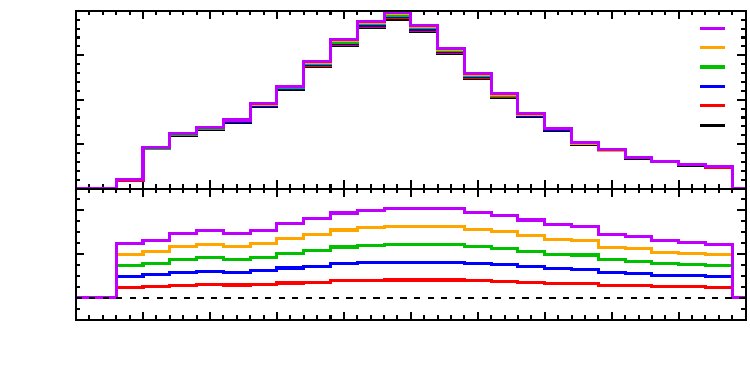
\includegraphics{nuenorm_E_RHC_sys1}}%
    \gplfronttext
  \end{picture}%
\endgroup
}
	\caption[Prediction of events with a simplified systematic model]%
		{Predictions of events at the far detector for the one ring $e$-like sample in %
		$\nu$-mode (left) and $\cj{\nu}$-mode (right), where %
		the $\nu_e$ (top) and $\cj{\nu}_e$ (bottom) CC cross-section systematics are applied %
		with relative errors between 1\,\% and 5\,\% at 1$\sigma$.
		In each figure, the top panel shows how the event distribution is affected, %
		and the bottom panel shows the variations with respect to the prediction without errors applied, %
		which is by definition one plus the $1\sigma$ histogram of the error, or $1 + f^n$ (see \refeq{eq:pull}). }
	\label{fig:nuenorm_prediction}
\end{figure}

\begin{figure}
	\centering
	\resizebox{0.49\linewidth}{!}{% GNUPLOT: LaTeX picture with Postscript
\begingroup
  \makeatletter
  \providecommand\color[2][]{%
    \GenericError{(gnuplot) \space\space\space\@spaces}{%
      Package color not loaded in conjunction with
      terminal option `colourtext'%
    }{See the gnuplot documentation for explanation.%
    }{Either use 'blacktext' in gnuplot or load the package
      color.sty in LaTeX.}%
    \renewcommand\color[2][]{}%
  }%
  \providecommand\includegraphics[2][]{%
    \GenericError{(gnuplot) \space\space\space\@spaces}{%
      Package graphicx or graphics not loaded%
    }{See the gnuplot documentation for explanation.%
    }{The gnuplot epslatex terminal needs graphicx.sty or graphics.sty.}%
    \renewcommand\includegraphics[2][]{}%
  }%
  \providecommand\rotatebox[2]{#2}%
  \@ifundefined{ifGPcolor}{%
    \newif\ifGPcolor
    \GPcolortrue
  }{}%
  \@ifundefined{ifGPblacktext}{%
    \newif\ifGPblacktext
    \GPblacktexttrue
  }{}%
  % define a \g@addto@macro without @ in the name:
  \let\gplgaddtomacro\g@addto@macro
  % define empty templates for all commands taking text:
  \gdef\gplbacktext{}%
  \gdef\gplfronttext{}%
  \makeatother
  \ifGPblacktext
    % no textcolor at all
    \def\colorrgb#1{}%
    \def\colorgray#1{}%
  \else
    % gray or color?
    \ifGPcolor
      \def\colorrgb#1{\color[rgb]{#1}}%
      \def\colorgray#1{\color[gray]{#1}}%
      \expandafter\def\csname LTw\endcsname{\color{white}}%
      \expandafter\def\csname LTb\endcsname{\color{black}}%
      \expandafter\def\csname LTa\endcsname{\color{black}}%
      \expandafter\def\csname LT0\endcsname{\color[rgb]{1,0,0}}%
      \expandafter\def\csname LT1\endcsname{\color[rgb]{0,1,0}}%
      \expandafter\def\csname LT2\endcsname{\color[rgb]{0,0,1}}%
      \expandafter\def\csname LT3\endcsname{\color[rgb]{1,0,1}}%
      \expandafter\def\csname LT4\endcsname{\color[rgb]{0,1,1}}%
      \expandafter\def\csname LT5\endcsname{\color[rgb]{1,1,0}}%
      \expandafter\def\csname LT6\endcsname{\color[rgb]{0,0,0}}%
      \expandafter\def\csname LT7\endcsname{\color[rgb]{1,0.3,0}}%
      \expandafter\def\csname LT8\endcsname{\color[rgb]{0.5,0.5,0.5}}%
    \else
      % gray
      \def\colorrgb#1{\color{black}}%
      \def\colorgray#1{\color[gray]{#1}}%
      \expandafter\def\csname LTw\endcsname{\color{white}}%
      \expandafter\def\csname LTb\endcsname{\color{black}}%
      \expandafter\def\csname LTa\endcsname{\color{black}}%
      \expandafter\def\csname LT0\endcsname{\color{black}}%
      \expandafter\def\csname LT1\endcsname{\color{black}}%
      \expandafter\def\csname LT2\endcsname{\color{black}}%
      \expandafter\def\csname LT3\endcsname{\color{black}}%
      \expandafter\def\csname LT4\endcsname{\color{black}}%
      \expandafter\def\csname LT5\endcsname{\color{black}}%
      \expandafter\def\csname LT6\endcsname{\color{black}}%
      \expandafter\def\csname LT7\endcsname{\color{black}}%
      \expandafter\def\csname LT8\endcsname{\color{black}}%
    \fi
  \fi
    \setlength{\unitlength}{0.0500bp}%
    \ifx\gptboxheight\undefined%
      \newlength{\gptboxheight}%
      \newlength{\gptboxwidth}%
      \newsavebox{\gptboxtext}%
    \fi%
    \setlength{\fboxrule}{0.5pt}%
    \setlength{\fboxsep}{1pt}%
\begin{picture}(10800.00,7560.00)%
    \gplgaddtomacro\gplbacktext{%
      \csname LTb\endcsname%%
      \put(870,1024){\makebox(0,0)[r]{\strut{}0}}%
      \csname LTb\endcsname%%
      \put(870,1713){\makebox(0,0)[r]{\strut{}1}}%
      \csname LTb\endcsname%%
      \put(870,2402){\makebox(0,0)[r]{\strut{}2}}%
      \csname LTb\endcsname%%
      \put(870,3091){\makebox(0,0)[r]{\strut{}3}}%
      \csname LTb\endcsname%%
      \put(1614,494){\makebox(0,0){\strut{}2.47}}%
      \csname LTb\endcsname%%
      \put(2683,494){\makebox(0,0){\strut{}2.48}}%
      \csname LTb\endcsname%%
      \put(3752,494){\makebox(0,0){\strut{}2.49}}%
      \csname LTb\endcsname%%
      \put(4821,494){\makebox(0,0){\strut{}2.5}}%
      \csname LTb\endcsname%%
      \put(5890,494){\makebox(0,0){\strut{}2.51}}%
      \csname LTb\endcsname%%
      \put(6960,494){\makebox(0,0){\strut{}2.52}}%
      \csname LTb\endcsname%%
      \put(8029,494){\makebox(0,0){\strut{}2.53}}%
      \csname LTb\endcsname%%
      \put(9098,494){\makebox(0,0){\strut{}2.54}}%
      \csname LTb\endcsname%%
      \put(10167,494){\makebox(0,0){\strut{}2.55}}%
    }%
    \gplgaddtomacro\gplfronttext{%
      \csname LTb\endcsname%%
      \put(582,2230){\rotatebox{-270}{\makebox(0,0){\strut{}$\Delta \chi^2 - \Delta \chi^2_0$}}}%
      \csname LTb\endcsname%%
      \put(5783,215){\makebox(0,0){\strut{}$\Delta m_{32}^2 / 10^{-3}$}}%
      \csname LTb\endcsname%%
      \put(6637,2998){\makebox(0,0){\strut{}Difference}}%
      \csname LTb\endcsname%%
      \put(6164,2812){\makebox(0,0)[l]{\strut{}$1\%$}}%
      \csname LTb\endcsname%%
      \put(6164,2626){\makebox(0,0)[l]{\strut{}$2\%$}}%
      \csname LTb\endcsname%%
      \put(6164,2440){\makebox(0,0)[l]{\strut{}$3\%$}}%
      \csname LTb\endcsname%%
      \put(6164,2254){\makebox(0,0)[l]{\strut{}$4\%$}}%
      \csname LTb\endcsname%%
      \put(6164,2068){\makebox(0,0)[l]{\strut{}$5\%$}}%
    }%
    \gplgaddtomacro\gplbacktext{%
      \csname LTb\endcsname%%
      \put(870,3780){\makebox(0,0)[r]{\strut{}0}}%
      \csname LTb\endcsname%%
      \put(870,4532){\makebox(0,0)[r]{\strut{}10}}%
      \csname LTb\endcsname%%
      \put(870,5284){\makebox(0,0)[r]{\strut{}20}}%
      \csname LTb\endcsname%%
      \put(870,6037){\makebox(0,0)[r]{\strut{}30}}%
      \csname LTb\endcsname%%
      \put(870,6789){\makebox(0,0)[r]{\strut{}40}}%
      \csname LTb\endcsname%%
      \put(1614,3594){\makebox(0,0){\strut{}}}%
      \csname LTb\endcsname%%
      \put(2683,3594){\makebox(0,0){\strut{}}}%
      \csname LTb\endcsname%%
      \put(3752,3594){\makebox(0,0){\strut{}}}%
      \csname LTb\endcsname%%
      \put(4821,3594){\makebox(0,0){\strut{}}}%
      \csname LTb\endcsname%%
      \put(5890,3594){\makebox(0,0){\strut{}}}%
      \csname LTb\endcsname%%
      \put(6960,3594){\makebox(0,0){\strut{}}}%
      \csname LTb\endcsname%%
      \put(8029,3594){\makebox(0,0){\strut{}}}%
      \csname LTb\endcsname%%
      \put(9098,3594){\makebox(0,0){\strut{}}}%
      \csname LTb\endcsname%%
      \put(10167,3594){\makebox(0,0){\strut{}}}%
    }%
    \gplgaddtomacro\gplfronttext{%
      \csname LTb\endcsname%%
      \put(480,5623){\rotatebox{-270}{\makebox(0,0){\strut{}$\Delta \chi^2$}}}%
      \csname LTb\endcsname%%
      \put(5783,3538){\makebox(0,0){\strut{}}}%
      \csname LTb\endcsname%%
      \put(6637,7004){\makebox(0,0){\strut{}}}%
      \csname LTb\endcsname%%
      \put(6164,7004){\makebox(0,0)[l]{\strut{}No syst}}%
      \csname LTb\endcsname%%
      \put(6164,6818){\makebox(0,0)[l]{\strut{}$1\%$}}%
      \csname LTb\endcsname%%
      \put(6164,6632){\makebox(0,0)[l]{\strut{}$2\%$}}%
      \csname LTb\endcsname%%
      \put(6164,6446){\makebox(0,0)[l]{\strut{}$3\%$}}%
      \csname LTb\endcsname%%
      \put(6164,6260){\makebox(0,0)[l]{\strut{}$4\%$}}%
      \csname LTb\endcsname%%
      \put(6164,6074){\makebox(0,0)[l]{\strut{}$5\%$}}%
    }%
    \gplbacktext
    \put(0,0){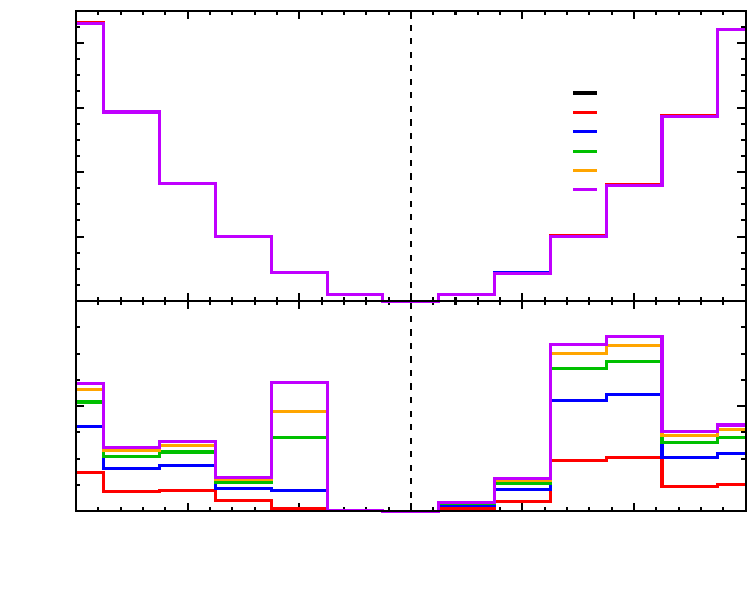
\includegraphics{pics/nuenorm_corr_chi2_M23}}%
    \gplfronttext
  \end{picture}%
\endgroup
}
	\resizebox{0.49\linewidth}{!}{% GNUPLOT: LaTeX picture with Postscript
\begingroup
  \makeatletter
  \providecommand\color[2][]{%
    \GenericError{(gnuplot) \space\space\space\@spaces}{%
      Package color not loaded in conjunction with
      terminal option `colourtext'%
    }{See the gnuplot documentation for explanation.%
    }{Either use 'blacktext' in gnuplot or load the package
      color.sty in LaTeX.}%
    \renewcommand\color[2][]{}%
  }%
  \providecommand\includegraphics[2][]{%
    \GenericError{(gnuplot) \space\space\space\@spaces}{%
      Package graphicx or graphics not loaded%
    }{See the gnuplot documentation for explanation.%
    }{The gnuplot epslatex terminal needs graphicx.sty or graphics.sty.}%
    \renewcommand\includegraphics[2][]{}%
  }%
  \providecommand\rotatebox[2]{#2}%
  \@ifundefined{ifGPcolor}{%
    \newif\ifGPcolor
    \GPcolortrue
  }{}%
  \@ifundefined{ifGPblacktext}{%
    \newif\ifGPblacktext
    \GPblacktexttrue
  }{}%
  % define a \g@addto@macro without @ in the name:
  \let\gplgaddtomacro\g@addto@macro
  % define empty templates for all commands taking text:
  \gdef\gplbacktext{}%
  \gdef\gplfronttext{}%
  \makeatother
  \ifGPblacktext
    % no textcolor at all
    \def\colorrgb#1{}%
    \def\colorgray#1{}%
  \else
    % gray or color?
    \ifGPcolor
      \def\colorrgb#1{\color[rgb]{#1}}%
      \def\colorgray#1{\color[gray]{#1}}%
      \expandafter\def\csname LTw\endcsname{\color{white}}%
      \expandafter\def\csname LTb\endcsname{\color{black}}%
      \expandafter\def\csname LTa\endcsname{\color{black}}%
      \expandafter\def\csname LT0\endcsname{\color[rgb]{1,0,0}}%
      \expandafter\def\csname LT1\endcsname{\color[rgb]{0,1,0}}%
      \expandafter\def\csname LT2\endcsname{\color[rgb]{0,0,1}}%
      \expandafter\def\csname LT3\endcsname{\color[rgb]{1,0,1}}%
      \expandafter\def\csname LT4\endcsname{\color[rgb]{0,1,1}}%
      \expandafter\def\csname LT5\endcsname{\color[rgb]{1,1,0}}%
      \expandafter\def\csname LT6\endcsname{\color[rgb]{0,0,0}}%
      \expandafter\def\csname LT7\endcsname{\color[rgb]{1,0.3,0}}%
      \expandafter\def\csname LT8\endcsname{\color[rgb]{0.5,0.5,0.5}}%
    \else
      % gray
      \def\colorrgb#1{\color{black}}%
      \def\colorgray#1{\color[gray]{#1}}%
      \expandafter\def\csname LTw\endcsname{\color{white}}%
      \expandafter\def\csname LTb\endcsname{\color{black}}%
      \expandafter\def\csname LTa\endcsname{\color{black}}%
      \expandafter\def\csname LT0\endcsname{\color{black}}%
      \expandafter\def\csname LT1\endcsname{\color{black}}%
      \expandafter\def\csname LT2\endcsname{\color{black}}%
      \expandafter\def\csname LT3\endcsname{\color{black}}%
      \expandafter\def\csname LT4\endcsname{\color{black}}%
      \expandafter\def\csname LT5\endcsname{\color{black}}%
      \expandafter\def\csname LT6\endcsname{\color{black}}%
      \expandafter\def\csname LT7\endcsname{\color{black}}%
      \expandafter\def\csname LT8\endcsname{\color{black}}%
    \fi
  \fi
    \setlength{\unitlength}{0.0500bp}%
    \ifx\gptboxheight\undefined%
      \newlength{\gptboxheight}%
      \newlength{\gptboxwidth}%
      \newsavebox{\gptboxtext}%
    \fi%
    \setlength{\fboxrule}{0.5pt}%
    \setlength{\fboxsep}{1pt}%
\begin{picture}(7200.00,5760.00)%
    \gplgaddtomacro\gplbacktext{%
      \csname LTb\endcsname%%
      \put(618,864){\makebox(0,0)[r]{\strut{}0}}%
      \csname LTb\endcsname%%
      \put(618,1368){\makebox(0,0)[r]{\strut{}1}}%
      \csname LTb\endcsname%%
      \put(618,1872){\makebox(0,0)[r]{\strut{}2}}%
      \csname LTb\endcsname%%
      \put(618,2376){\makebox(0,0)[r]{\strut{}3}}%
      \csname LTb\endcsname%%
      \put(720,678){\makebox(0,0){\strut{}2.464}}%
      \csname LTb\endcsname%%
      \put(1791,678){\makebox(0,0){\strut{}2.479}}%
      \csname LTb\endcsname%%
      \put(2863,678){\makebox(0,0){\strut{}2.494}}%
      \csname LTb\endcsname%%
      \put(3934,678){\makebox(0,0){\strut{}2.509}}%
      \csname LTb\endcsname%%
      \put(5005,678){\makebox(0,0){\strut{}2.524}}%
      \csname LTb\endcsname%%
      \put(6077,678){\makebox(0,0){\strut{}2.539}}%
      \csname LTb\endcsname%%
      \put(7148,678){\makebox(0,0){\strut{}2.554}}%
    }%
    \gplgaddtomacro\gplfronttext{%
      \csname LTb\endcsname%%
      \put(330,1872){\rotatebox{-270}{\makebox(0,0){\strut{}$\Delta \chi^2_\text{No syst} - \Delta \chi^2$}}}%
      \csname LTb\endcsname%%
      \put(3934,399){\makebox(0,0){\strut{}$\Delta m_{32}^2 / 10^{-3}$}}%
    }%
    \gplgaddtomacro\gplbacktext{%
      \csname LTb\endcsname%%
      \put(618,2880){\makebox(0,0)[r]{\strut{}0}}%
      \csname LTb\endcsname%%
      \put(618,3499){\makebox(0,0)[r]{\strut{}10}}%
      \csname LTb\endcsname%%
      \put(618,4118){\makebox(0,0)[r]{\strut{}20}}%
      \csname LTb\endcsname%%
      \put(618,4737){\makebox(0,0)[r]{\strut{}30}}%
      \csname LTb\endcsname%%
      \put(618,5356){\makebox(0,0)[r]{\strut{}40}}%
      \csname LTb\endcsname%%
      \put(720,2694){\makebox(0,0){\strut{}}}%
      \csname LTb\endcsname%%
      \put(1791,2694){\makebox(0,0){\strut{}}}%
      \csname LTb\endcsname%%
      \put(2863,2694){\makebox(0,0){\strut{}}}%
      \csname LTb\endcsname%%
      \put(3934,2694){\makebox(0,0){\strut{}}}%
      \csname LTb\endcsname%%
      \put(5005,2694){\makebox(0,0){\strut{}}}%
      \csname LTb\endcsname%%
      \put(6077,2694){\makebox(0,0){\strut{}}}%
      \csname LTb\endcsname%%
      \put(7148,2694){\makebox(0,0){\strut{}}}%
    }%
    \gplgaddtomacro\gplfronttext{%
      \csname LTb\endcsname%%
      \put(228,4273){\rotatebox{-270}{\makebox(0,0){\strut{}$\Delta \chi^2$}}}%
      \csname LTb\endcsname%%
      \put(3934,2638){\makebox(0,0){\strut{}}}%
      \csname LTb\endcsname%%
      \put(4941,4877){\makebox(0,0){\strut{}}}%
      \csname LTb\endcsname%%
      \put(5389,4877){\makebox(0,0)[r]{\strut{}No syst}}%
      \csname LTb\endcsname%%
      \put(5389,4691){\makebox(0,0)[r]{\strut{}1\,\%}}%
      \csname LTb\endcsname%%
      \put(5389,4505){\makebox(0,0)[r]{\strut{}2\,\%}}%
      \csname LTb\endcsname%%
      \put(5389,4319){\makebox(0,0)[r]{\strut{}3\,\%}}%
      \csname LTb\endcsname%%
      \put(5389,4133){\makebox(0,0)[r]{\strut{}4\,\%}}%
      \csname LTb\endcsname%%
      \put(5389,3947){\makebox(0,0)[r]{\strut{}5\,\%}}%
    }%
    \gplbacktext
    \put(0,0){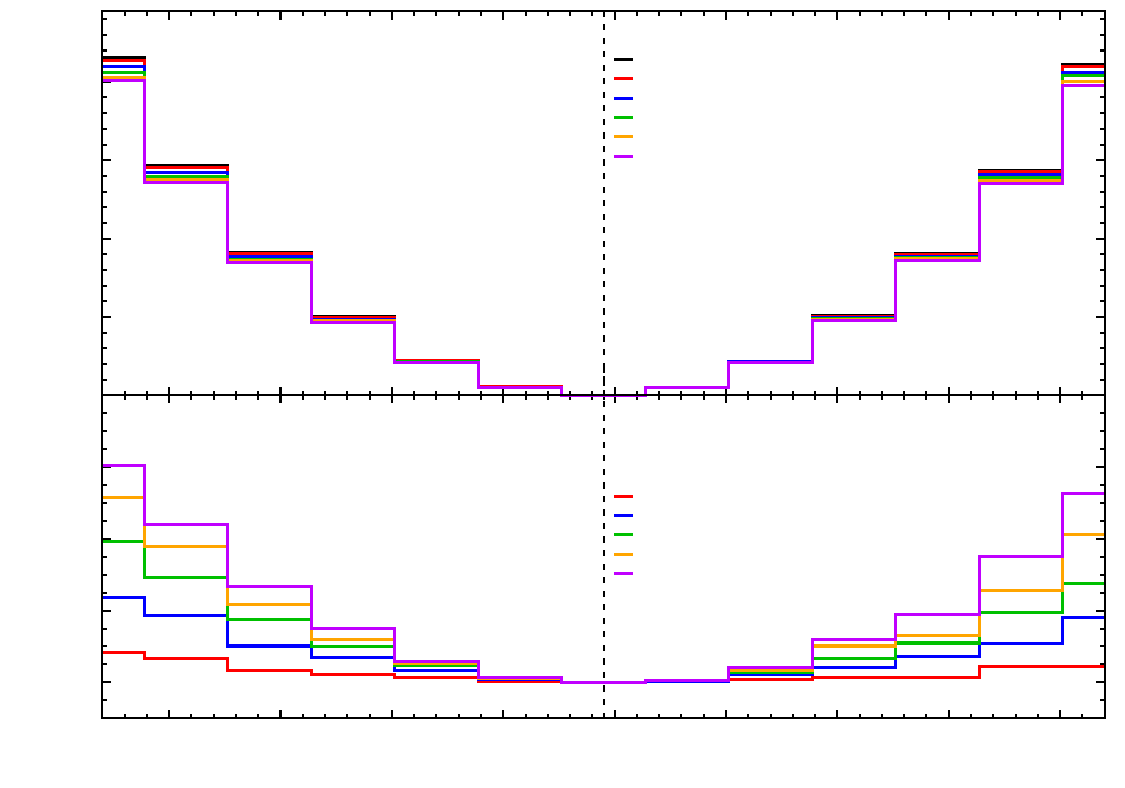
\includegraphics{pics/nuenorm_anti_chi2_M23}}%
    \gplfronttext
  \end{picture}%
\endgroup
}
	\resizebox{0.49\linewidth}{!}{% GNUPLOT: LaTeX picture with Postscript
\begingroup
  \makeatletter
  \providecommand\color[2][]{%
    \GenericError{(gnuplot) \space\space\space\@spaces}{%
      Package color not loaded in conjunction with
      terminal option `colourtext'%
    }{See the gnuplot documentation for explanation.%
    }{Either use 'blacktext' in gnuplot or load the package
      color.sty in LaTeX.}%
    \renewcommand\color[2][]{}%
  }%
  \providecommand\includegraphics[2][]{%
    \GenericError{(gnuplot) \space\space\space\@spaces}{%
      Package graphicx or graphics not loaded%
    }{See the gnuplot documentation for explanation.%
    }{The gnuplot epslatex terminal needs graphicx.sty or graphics.sty.}%
    \renewcommand\includegraphics[2][]{}%
  }%
  \providecommand\rotatebox[2]{#2}%
  \@ifundefined{ifGPcolor}{%
    \newif\ifGPcolor
    \GPcolortrue
  }{}%
  \@ifundefined{ifGPblacktext}{%
    \newif\ifGPblacktext
    \GPblacktexttrue
  }{}%
  % define a \g@addto@macro without @ in the name:
  \let\gplgaddtomacro\g@addto@macro
  % define empty templates for all commands taking text:
  \gdef\gplbacktext{}%
  \gdef\gplfronttext{}%
  \makeatother
  \ifGPblacktext
    % no textcolor at all
    \def\colorrgb#1{}%
    \def\colorgray#1{}%
  \else
    % gray or color?
    \ifGPcolor
      \def\colorrgb#1{\color[rgb]{#1}}%
      \def\colorgray#1{\color[gray]{#1}}%
      \expandafter\def\csname LTw\endcsname{\color{white}}%
      \expandafter\def\csname LTb\endcsname{\color{black}}%
      \expandafter\def\csname LTa\endcsname{\color{black}}%
      \expandafter\def\csname LT0\endcsname{\color[rgb]{1,0,0}}%
      \expandafter\def\csname LT1\endcsname{\color[rgb]{0,1,0}}%
      \expandafter\def\csname LT2\endcsname{\color[rgb]{0,0,1}}%
      \expandafter\def\csname LT3\endcsname{\color[rgb]{1,0,1}}%
      \expandafter\def\csname LT4\endcsname{\color[rgb]{0,1,1}}%
      \expandafter\def\csname LT5\endcsname{\color[rgb]{1,1,0}}%
      \expandafter\def\csname LT6\endcsname{\color[rgb]{0,0,0}}%
      \expandafter\def\csname LT7\endcsname{\color[rgb]{1,0.3,0}}%
      \expandafter\def\csname LT8\endcsname{\color[rgb]{0.5,0.5,0.5}}%
    \else
      % gray
      \def\colorrgb#1{\color{black}}%
      \def\colorgray#1{\color[gray]{#1}}%
      \expandafter\def\csname LTw\endcsname{\color{white}}%
      \expandafter\def\csname LTb\endcsname{\color{black}}%
      \expandafter\def\csname LTa\endcsname{\color{black}}%
      \expandafter\def\csname LT0\endcsname{\color{black}}%
      \expandafter\def\csname LT1\endcsname{\color{black}}%
      \expandafter\def\csname LT2\endcsname{\color{black}}%
      \expandafter\def\csname LT3\endcsname{\color{black}}%
      \expandafter\def\csname LT4\endcsname{\color{black}}%
      \expandafter\def\csname LT5\endcsname{\color{black}}%
      \expandafter\def\csname LT6\endcsname{\color{black}}%
      \expandafter\def\csname LT7\endcsname{\color{black}}%
      \expandafter\def\csname LT8\endcsname{\color{black}}%
    \fi
  \fi
    \setlength{\unitlength}{0.0500bp}%
    \ifx\gptboxheight\undefined%
      \newlength{\gptboxheight}%
      \newlength{\gptboxwidth}%
      \newsavebox{\gptboxtext}%
    \fi%
    \setlength{\fboxrule}{0.5pt}%
    \setlength{\fboxsep}{1pt}%
\begin{picture}(7200.00,5760.00)%
    \gplgaddtomacro\gplbacktext{%
      \csname LTb\endcsname%%
      \put(618,864){\makebox(0,0)[r]{\strut{}0}}%
      \csname LTb\endcsname%%
      \put(618,1200){\makebox(0,0)[r]{\strut{}10}}%
      \csname LTb\endcsname%%
      \put(618,1536){\makebox(0,0)[r]{\strut{}20}}%
      \csname LTb\endcsname%%
      \put(618,1872){\makebox(0,0)[r]{\strut{}30}}%
      \csname LTb\endcsname%%
      \put(618,2208){\makebox(0,0)[r]{\strut{}40}}%
      \csname LTb\endcsname%%
      \put(618,2544){\makebox(0,0)[r]{\strut{}50}}%
      \csname LTb\endcsname%%
      \put(720,678){\makebox(0,0){\strut{}0.07}}%
      \csname LTb\endcsname%%
      \put(1791,678){\makebox(0,0){\strut{}0.075}}%
      \csname LTb\endcsname%%
      \put(2863,678){\makebox(0,0){\strut{}0.08}}%
      \csname LTb\endcsname%%
      \put(3934,678){\makebox(0,0){\strut{}0.085}}%
      \csname LTb\endcsname%%
      \put(5005,678){\makebox(0,0){\strut{}0.09}}%
      \csname LTb\endcsname%%
      \put(6077,678){\makebox(0,0){\strut{}0.095}}%
      \csname LTb\endcsname%%
      \put(7148,678){\makebox(0,0){\strut{}0.1}}%
    }%
    \gplgaddtomacro\gplfronttext{%
      \csname LTb\endcsname%%
      \put(228,1872){\rotatebox{-270}{\makebox(0,0){\strut{}$\Delta \chi^2_\text{No syst} - \Delta \chi^2$}}}%
      \csname LTb\endcsname%%
      \put(3934,399){\makebox(0,0){\strut{}$\sin^2 2 \theta_{13}$}}%
    }%
    \gplgaddtomacro\gplbacktext{%
      \csname LTb\endcsname%%
      \put(618,2880){\makebox(0,0)[r]{\strut{}0}}%
      \csname LTb\endcsname%%
      \put(618,3577){\makebox(0,0)[r]{\strut{}20}}%
      \csname LTb\endcsname%%
      \put(618,4273){\makebox(0,0)[r]{\strut{}40}}%
      \csname LTb\endcsname%%
      \put(618,4970){\makebox(0,0)[r]{\strut{}60}}%
      \csname LTb\endcsname%%
      \put(618,5666){\makebox(0,0)[r]{\strut{}80}}%
      \csname LTb\endcsname%%
      \put(720,2694){\makebox(0,0){\strut{}}}%
      \csname LTb\endcsname%%
      \put(1791,2694){\makebox(0,0){\strut{}}}%
      \csname LTb\endcsname%%
      \put(2863,2694){\makebox(0,0){\strut{}}}%
      \csname LTb\endcsname%%
      \put(3934,2694){\makebox(0,0){\strut{}}}%
      \csname LTb\endcsname%%
      \put(5005,2694){\makebox(0,0){\strut{}}}%
      \csname LTb\endcsname%%
      \put(6077,2694){\makebox(0,0){\strut{}}}%
      \csname LTb\endcsname%%
      \put(7148,2694){\makebox(0,0){\strut{}}}%
    }%
    \gplgaddtomacro\gplfronttext{%
      \csname LTb\endcsname%%
      \put(228,4273){\rotatebox{-270}{\makebox(0,0){\strut{}$\Delta \chi^2$}}}%
      \csname LTb\endcsname%%
      \put(3934,2638){\makebox(0,0){\strut{}}}%
      \csname LTb\endcsname%%
      \put(4954,4877){\makebox(0,0){\strut{}}}%
      \csname LTb\endcsname%%
      \put(5402,4877){\makebox(0,0)[r]{\strut{}No syst}}%
      \csname LTb\endcsname%%
      \put(5402,4691){\makebox(0,0)[r]{\strut{}1\,\%}}%
      \csname LTb\endcsname%%
      \put(5402,4505){\makebox(0,0)[r]{\strut{}2\,\%}}%
      \csname LTb\endcsname%%
      \put(5402,4319){\makebox(0,0)[r]{\strut{}3\,\%}}%
      \csname LTb\endcsname%%
      \put(5402,4133){\makebox(0,0)[r]{\strut{}4\,\%}}%
      \csname LTb\endcsname%%
      \put(5402,3947){\makebox(0,0)[r]{\strut{}5\,\%}}%
    }%
    \gplbacktext
    \put(0,0){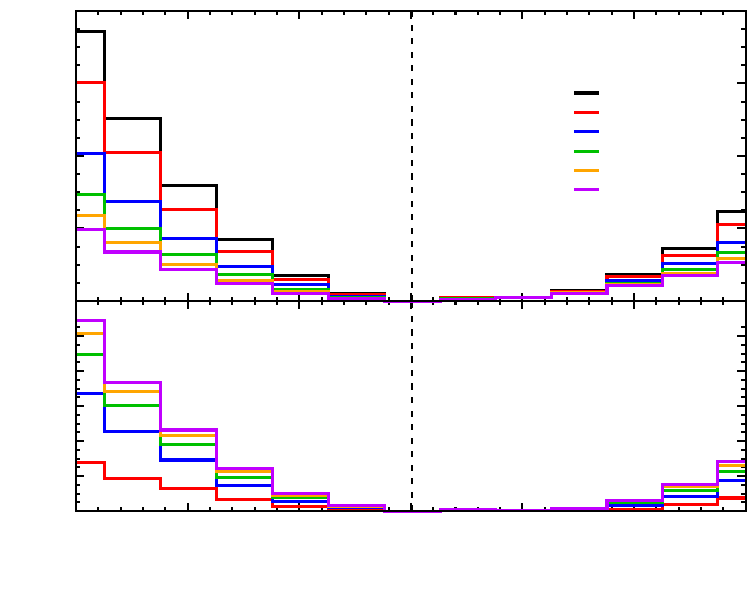
\includegraphics{pics/nuenorm_corr_chi2_S13}}%
    \gplfronttext
  \end{picture}%
\endgroup
}
	\resizebox{0.49\linewidth}{!}{% GNUPLOT: LaTeX picture with Postscript
\begingroup
  \makeatletter
  \providecommand\color[2][]{%
    \GenericError{(gnuplot) \space\space\space\@spaces}{%
      Package color not loaded in conjunction with
      terminal option `colourtext'%
    }{See the gnuplot documentation for explanation.%
    }{Either use 'blacktext' in gnuplot or load the package
      color.sty in LaTeX.}%
    \renewcommand\color[2][]{}%
  }%
  \providecommand\includegraphics[2][]{%
    \GenericError{(gnuplot) \space\space\space\@spaces}{%
      Package graphicx or graphics not loaded%
    }{See the gnuplot documentation for explanation.%
    }{The gnuplot epslatex terminal needs graphicx.sty or graphics.sty.}%
    \renewcommand\includegraphics[2][]{}%
  }%
  \providecommand\rotatebox[2]{#2}%
  \@ifundefined{ifGPcolor}{%
    \newif\ifGPcolor
    \GPcolortrue
  }{}%
  \@ifundefined{ifGPblacktext}{%
    \newif\ifGPblacktext
    \GPblacktexttrue
  }{}%
  % define a \g@addto@macro without @ in the name:
  \let\gplgaddtomacro\g@addto@macro
  % define empty templates for all commands taking text:
  \gdef\gplbacktext{}%
  \gdef\gplfronttext{}%
  \makeatother
  \ifGPblacktext
    % no textcolor at all
    \def\colorrgb#1{}%
    \def\colorgray#1{}%
  \else
    % gray or color?
    \ifGPcolor
      \def\colorrgb#1{\color[rgb]{#1}}%
      \def\colorgray#1{\color[gray]{#1}}%
      \expandafter\def\csname LTw\endcsname{\color{white}}%
      \expandafter\def\csname LTb\endcsname{\color{black}}%
      \expandafter\def\csname LTa\endcsname{\color{black}}%
      \expandafter\def\csname LT0\endcsname{\color[rgb]{1,0,0}}%
      \expandafter\def\csname LT1\endcsname{\color[rgb]{0,1,0}}%
      \expandafter\def\csname LT2\endcsname{\color[rgb]{0,0,1}}%
      \expandafter\def\csname LT3\endcsname{\color[rgb]{1,0,1}}%
      \expandafter\def\csname LT4\endcsname{\color[rgb]{0,1,1}}%
      \expandafter\def\csname LT5\endcsname{\color[rgb]{1,1,0}}%
      \expandafter\def\csname LT6\endcsname{\color[rgb]{0,0,0}}%
      \expandafter\def\csname LT7\endcsname{\color[rgb]{1,0.3,0}}%
      \expandafter\def\csname LT8\endcsname{\color[rgb]{0.5,0.5,0.5}}%
    \else
      % gray
      \def\colorrgb#1{\color{black}}%
      \def\colorgray#1{\color[gray]{#1}}%
      \expandafter\def\csname LTw\endcsname{\color{white}}%
      \expandafter\def\csname LTb\endcsname{\color{black}}%
      \expandafter\def\csname LTa\endcsname{\color{black}}%
      \expandafter\def\csname LT0\endcsname{\color{black}}%
      \expandafter\def\csname LT1\endcsname{\color{black}}%
      \expandafter\def\csname LT2\endcsname{\color{black}}%
      \expandafter\def\csname LT3\endcsname{\color{black}}%
      \expandafter\def\csname LT4\endcsname{\color{black}}%
      \expandafter\def\csname LT5\endcsname{\color{black}}%
      \expandafter\def\csname LT6\endcsname{\color{black}}%
      \expandafter\def\csname LT7\endcsname{\color{black}}%
      \expandafter\def\csname LT8\endcsname{\color{black}}%
    \fi
  \fi
    \setlength{\unitlength}{0.0500bp}%
    \ifx\gptboxheight\undefined%
      \newlength{\gptboxheight}%
      \newlength{\gptboxwidth}%
      \newsavebox{\gptboxtext}%
    \fi%
    \setlength{\fboxrule}{0.5pt}%
    \setlength{\fboxsep}{1pt}%
\begin{picture}(7200.00,5760.00)%
    \gplgaddtomacro\gplbacktext{%
      \csname LTb\endcsname%%
      \put(618,864){\makebox(0,0)[r]{\strut{}0}}%
      \csname LTb\endcsname%%
      \put(618,1872){\makebox(0,0)[r]{\strut{}10}}%
      \csname LTb\endcsname%%
      \put(720,678){\makebox(0,0){\strut{}0.07}}%
      \csname LTb\endcsname%%
      \put(1791,678){\makebox(0,0){\strut{}0.075}}%
      \csname LTb\endcsname%%
      \put(2863,678){\makebox(0,0){\strut{}0.08}}%
      \csname LTb\endcsname%%
      \put(3934,678){\makebox(0,0){\strut{}0.085}}%
      \csname LTb\endcsname%%
      \put(5005,678){\makebox(0,0){\strut{}0.09}}%
      \csname LTb\endcsname%%
      \put(6077,678){\makebox(0,0){\strut{}0.095}}%
      \csname LTb\endcsname%%
      \put(7148,678){\makebox(0,0){\strut{}0.1}}%
    }%
    \gplgaddtomacro\gplfronttext{%
      \csname LTb\endcsname%%
      \put(228,1872){\rotatebox{-270}{\makebox(0,0){\strut{}$\Delta \chi^2_\text{No syst} - \Delta \chi^2$}}}%
      \csname LTb\endcsname%%
      \put(3934,399){\makebox(0,0){\strut{}$\sin^2 2 \theta_{13}$}}%
    }%
    \gplgaddtomacro\gplbacktext{%
      \csname LTb\endcsname%%
      \put(618,2880){\makebox(0,0)[r]{\strut{}0}}%
      \csname LTb\endcsname%%
      \put(618,3577){\makebox(0,0)[r]{\strut{}20}}%
      \csname LTb\endcsname%%
      \put(618,4273){\makebox(0,0)[r]{\strut{}40}}%
      \csname LTb\endcsname%%
      \put(618,4970){\makebox(0,0)[r]{\strut{}60}}%
      \csname LTb\endcsname%%
      \put(618,5666){\makebox(0,0)[r]{\strut{}80}}%
      \csname LTb\endcsname%%
      \put(720,2694){\makebox(0,0){\strut{}}}%
      \csname LTb\endcsname%%
      \put(1791,2694){\makebox(0,0){\strut{}}}%
      \csname LTb\endcsname%%
      \put(2863,2694){\makebox(0,0){\strut{}}}%
      \csname LTb\endcsname%%
      \put(3934,2694){\makebox(0,0){\strut{}}}%
      \csname LTb\endcsname%%
      \put(5005,2694){\makebox(0,0){\strut{}}}%
      \csname LTb\endcsname%%
      \put(6077,2694){\makebox(0,0){\strut{}}}%
      \csname LTb\endcsname%%
      \put(7148,2694){\makebox(0,0){\strut{}}}%
    }%
    \gplgaddtomacro\gplfronttext{%
      \csname LTb\endcsname%%
      \put(228,4273){\rotatebox{-270}{\makebox(0,0){\strut{}$\Delta \chi^2$}}}%
      \csname LTb\endcsname%%
      \put(3934,2638){\makebox(0,0){\strut{}}}%
      \csname LTb\endcsname%%
      \put(4954,4877){\makebox(0,0){\strut{}}}%
      \csname LTb\endcsname%%
      \put(5402,4877){\makebox(0,0)[r]{\strut{}No syst}}%
      \csname LTb\endcsname%%
      \put(5402,4691){\makebox(0,0)[r]{\strut{}1\,\%}}%
      \csname LTb\endcsname%%
      \put(5402,4505){\makebox(0,0)[r]{\strut{}2\,\%}}%
      \csname LTb\endcsname%%
      \put(5402,4319){\makebox(0,0)[r]{\strut{}3\,\%}}%
      \csname LTb\endcsname%%
      \put(5402,4133){\makebox(0,0)[r]{\strut{}4\,\%}}%
      \csname LTb\endcsname%%
      \put(5402,3947){\makebox(0,0)[r]{\strut{}5\,\%}}%
    }%
    \gplbacktext
    \put(0,0){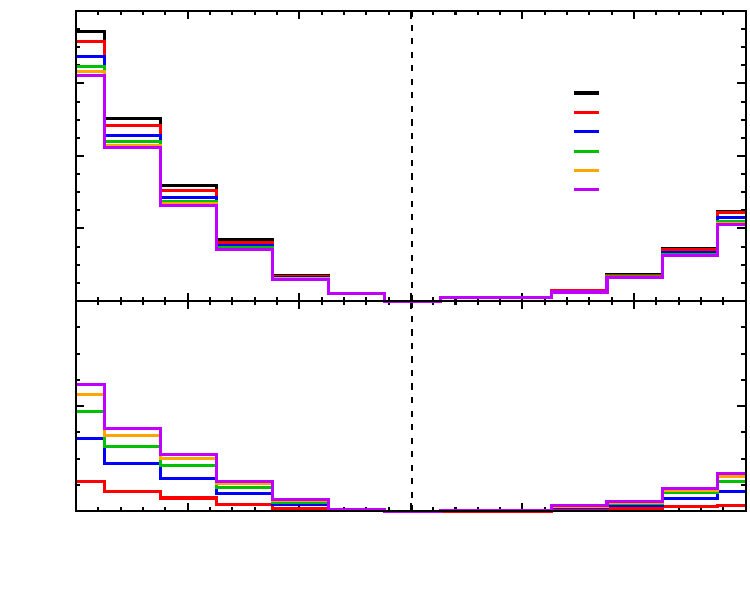
\includegraphics{pics/nuenorm_anti_chi2_S13}}%
    \gplfronttext
  \end{picture}%
\endgroup
}
	\resizebox{0.49\linewidth}{!}{% GNUPLOT: LaTeX picture with Postscript
\begingroup
  \makeatletter
  \providecommand\color[2][]{%
    \GenericError{(gnuplot) \space\space\space\@spaces}{%
      Package color not loaded in conjunction with
      terminal option `colourtext'%
    }{See the gnuplot documentation for explanation.%
    }{Either use 'blacktext' in gnuplot or load the package
      color.sty in LaTeX.}%
    \renewcommand\color[2][]{}%
  }%
  \providecommand\includegraphics[2][]{%
    \GenericError{(gnuplot) \space\space\space\@spaces}{%
      Package graphicx or graphics not loaded%
    }{See the gnuplot documentation for explanation.%
    }{The gnuplot epslatex terminal needs graphicx.sty or graphics.sty.}%
    \renewcommand\includegraphics[2][]{}%
  }%
  \providecommand\rotatebox[2]{#2}%
  \@ifundefined{ifGPcolor}{%
    \newif\ifGPcolor
    \GPcolortrue
  }{}%
  \@ifundefined{ifGPblacktext}{%
    \newif\ifGPblacktext
    \GPblacktexttrue
  }{}%
  % define a \g@addto@macro without @ in the name:
  \let\gplgaddtomacro\g@addto@macro
  % define empty templates for all commands taking text:
  \gdef\gplbacktext{}%
  \gdef\gplfronttext{}%
  \makeatother
  \ifGPblacktext
    % no textcolor at all
    \def\colorrgb#1{}%
    \def\colorgray#1{}%
  \else
    % gray or color?
    \ifGPcolor
      \def\colorrgb#1{\color[rgb]{#1}}%
      \def\colorgray#1{\color[gray]{#1}}%
      \expandafter\def\csname LTw\endcsname{\color{white}}%
      \expandafter\def\csname LTb\endcsname{\color{black}}%
      \expandafter\def\csname LTa\endcsname{\color{black}}%
      \expandafter\def\csname LT0\endcsname{\color[rgb]{1,0,0}}%
      \expandafter\def\csname LT1\endcsname{\color[rgb]{0,1,0}}%
      \expandafter\def\csname LT2\endcsname{\color[rgb]{0,0,1}}%
      \expandafter\def\csname LT3\endcsname{\color[rgb]{1,0,1}}%
      \expandafter\def\csname LT4\endcsname{\color[rgb]{0,1,1}}%
      \expandafter\def\csname LT5\endcsname{\color[rgb]{1,1,0}}%
      \expandafter\def\csname LT6\endcsname{\color[rgb]{0,0,0}}%
      \expandafter\def\csname LT7\endcsname{\color[rgb]{1,0.3,0}}%
      \expandafter\def\csname LT8\endcsname{\color[rgb]{0.5,0.5,0.5}}%
    \else
      % gray
      \def\colorrgb#1{\color{black}}%
      \def\colorgray#1{\color[gray]{#1}}%
      \expandafter\def\csname LTw\endcsname{\color{white}}%
      \expandafter\def\csname LTb\endcsname{\color{black}}%
      \expandafter\def\csname LTa\endcsname{\color{black}}%
      \expandafter\def\csname LT0\endcsname{\color{black}}%
      \expandafter\def\csname LT1\endcsname{\color{black}}%
      \expandafter\def\csname LT2\endcsname{\color{black}}%
      \expandafter\def\csname LT3\endcsname{\color{black}}%
      \expandafter\def\csname LT4\endcsname{\color{black}}%
      \expandafter\def\csname LT5\endcsname{\color{black}}%
      \expandafter\def\csname LT6\endcsname{\color{black}}%
      \expandafter\def\csname LT7\endcsname{\color{black}}%
      \expandafter\def\csname LT8\endcsname{\color{black}}%
    \fi
  \fi
    \setlength{\unitlength}{0.0500bp}%
    \ifx\gptboxheight\undefined%
      \newlength{\gptboxheight}%
      \newlength{\gptboxwidth}%
      \newsavebox{\gptboxtext}%
    \fi%
    \setlength{\fboxrule}{0.5pt}%
    \setlength{\fboxsep}{1pt}%
\begin{picture}(10800.00,7560.00)%
    \gplgaddtomacro\gplbacktext{%
      \csname LTb\endcsname%%
      \put(870,874){\makebox(0,0)[r]{\strut{}0}}%
      \csname LTb\endcsname%%
      \put(870,1358){\makebox(0,0)[r]{\strut{}5}}%
      \csname LTb\endcsname%%
      \put(870,1843){\makebox(0,0)[r]{\strut{}10}}%
      \csname LTb\endcsname%%
      \put(870,2327){\makebox(0,0)[r]{\strut{}15}}%
      \csname LTb\endcsname%%
      \put(870,2811){\makebox(0,0)[r]{\strut{}20}}%
      \csname LTb\endcsname%%
      \put(870,3296){\makebox(0,0)[r]{\strut{}25}}%
      \csname LTb\endcsname%%
      \put(1853,494){\makebox(0,0){\strut{}0.44}}%
      \csname LTb\endcsname%%
      \put(3110,494){\makebox(0,0){\strut{}0.46}}%
      \csname LTb\endcsname%%
      \put(4368,494){\makebox(0,0){\strut{}0.48}}%
      \csname LTb\endcsname%%
      \put(5626,494){\makebox(0,0){\strut{}0.5}}%
      \csname LTb\endcsname%%
      \put(6884,494){\makebox(0,0){\strut{}0.52}}%
      \csname LTb\endcsname%%
      \put(8142,494){\makebox(0,0){\strut{}0.54}}%
      \csname LTb\endcsname%%
      \put(9400,494){\makebox(0,0){\strut{}0.56}}%
    }%
    \gplgaddtomacro\gplfronttext{%
      \csname LTb\endcsname%%
      \put(480,2230){\rotatebox{-270}{\makebox(0,0){\strut{}$\Delta \chi^2 - \Delta \chi^2_0$}}}%
      \csname LTb\endcsname%%
      \put(5783,215){\makebox(0,0){\strut{}$\sin^2 \theta_{23}$}}%
      \csname LTb\endcsname%%
      \put(8240,2718){\makebox(0,0){\strut{}Difference}}%
      \csname LTb\endcsname%%
      \put(7767,2532){\makebox(0,0)[l]{\strut{}$1\%$}}%
      \csname LTb\endcsname%%
      \put(7767,2346){\makebox(0,0)[l]{\strut{}$2\%$}}%
      \csname LTb\endcsname%%
      \put(7767,2160){\makebox(0,0)[l]{\strut{}$3\%$}}%
      \csname LTb\endcsname%%
      \put(7767,1974){\makebox(0,0)[l]{\strut{}$4\%$}}%
      \csname LTb\endcsname%%
      \put(7767,1788){\makebox(0,0)[l]{\strut{}$5\%$}}%
    }%
    \gplgaddtomacro\gplbacktext{%
      \csname LTb\endcsname%%
      \put(870,3780){\makebox(0,0)[r]{\strut{}0}}%
      \csname LTb\endcsname%%
      \put(870,4242){\makebox(0,0)[r]{\strut{}50}}%
      \csname LTb\endcsname%%
      \put(870,4704){\makebox(0,0)[r]{\strut{}100}}%
      \csname LTb\endcsname%%
      \put(870,5166){\makebox(0,0)[r]{\strut{}150}}%
      \csname LTb\endcsname%%
      \put(870,5628){\makebox(0,0)[r]{\strut{}200}}%
      \csname LTb\endcsname%%
      \put(870,6090){\makebox(0,0)[r]{\strut{}250}}%
      \csname LTb\endcsname%%
      \put(870,6551){\makebox(0,0)[r]{\strut{}300}}%
      \csname LTb\endcsname%%
      \put(870,7013){\makebox(0,0)[r]{\strut{}350}}%
      \csname LTb\endcsname%%
      \put(1853,3594){\makebox(0,0){\strut{}}}%
      \csname LTb\endcsname%%
      \put(3110,3594){\makebox(0,0){\strut{}}}%
      \csname LTb\endcsname%%
      \put(4368,3594){\makebox(0,0){\strut{}}}%
      \csname LTb\endcsname%%
      \put(5626,3594){\makebox(0,0){\strut{}}}%
      \csname LTb\endcsname%%
      \put(6884,3594){\makebox(0,0){\strut{}}}%
      \csname LTb\endcsname%%
      \put(8142,3594){\makebox(0,0){\strut{}}}%
      \csname LTb\endcsname%%
      \put(9400,3594){\makebox(0,0){\strut{}}}%
    }%
    \gplgaddtomacro\gplfronttext{%
      \csname LTb\endcsname%%
      \put(378,5623){\rotatebox{-270}{\makebox(0,0){\strut{}$\Delta \chi^2$}}}%
      \csname LTb\endcsname%%
      \put(5783,3538){\makebox(0,0){\strut{}}}%
      \csname LTb\endcsname%%
      \put(8240,7004){\makebox(0,0){\strut{}}}%
      \csname LTb\endcsname%%
      \put(7767,7004){\makebox(0,0)[l]{\strut{}No syst}}%
      \csname LTb\endcsname%%
      \put(7767,6818){\makebox(0,0)[l]{\strut{}$1\%$}}%
      \csname LTb\endcsname%%
      \put(7767,6632){\makebox(0,0)[l]{\strut{}$2\%$}}%
      \csname LTb\endcsname%%
      \put(7767,6446){\makebox(0,0)[l]{\strut{}$3\%$}}%
      \csname LTb\endcsname%%
      \put(7767,6260){\makebox(0,0)[l]{\strut{}$4\%$}}%
      \csname LTb\endcsname%%
      \put(7767,6074){\makebox(0,0)[l]{\strut{}$5\%$}}%
    }%
    \gplbacktext
    \put(0,0){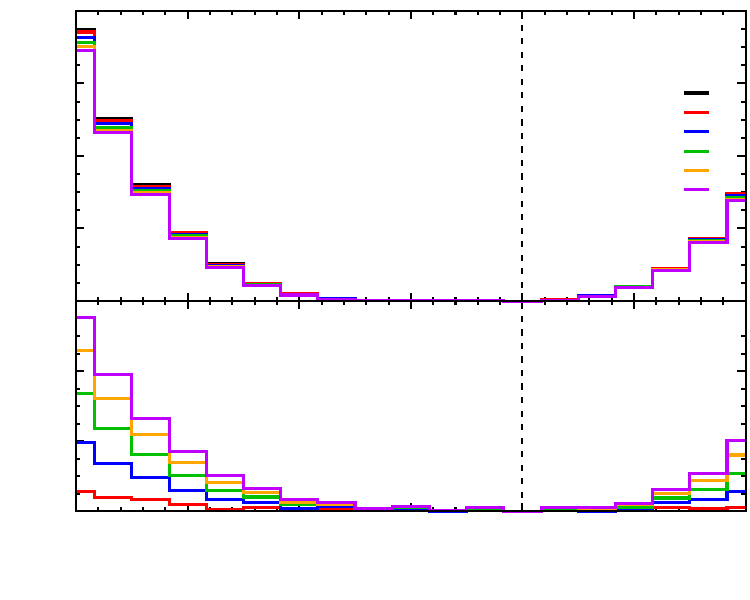
\includegraphics{pics/nuenorm_corr_chi2_S23}}%
    \gplfronttext
  \end{picture}%
\endgroup
}
	\resizebox{0.49\linewidth}{!}{% GNUPLOT: LaTeX picture with Postscript
\begingroup
  \makeatletter
  \providecommand\color[2][]{%
    \GenericError{(gnuplot) \space\space\space\@spaces}{%
      Package color not loaded in conjunction with
      terminal option `colourtext'%
    }{See the gnuplot documentation for explanation.%
    }{Either use 'blacktext' in gnuplot or load the package
      color.sty in LaTeX.}%
    \renewcommand\color[2][]{}%
  }%
  \providecommand\includegraphics[2][]{%
    \GenericError{(gnuplot) \space\space\space\@spaces}{%
      Package graphicx or graphics not loaded%
    }{See the gnuplot documentation for explanation.%
    }{The gnuplot epslatex terminal needs graphicx.sty or graphics.sty.}%
    \renewcommand\includegraphics[2][]{}%
  }%
  \providecommand\rotatebox[2]{#2}%
  \@ifundefined{ifGPcolor}{%
    \newif\ifGPcolor
    \GPcolortrue
  }{}%
  \@ifundefined{ifGPblacktext}{%
    \newif\ifGPblacktext
    \GPblacktexttrue
  }{}%
  % define a \g@addto@macro without @ in the name:
  \let\gplgaddtomacro\g@addto@macro
  % define empty templates for all commands taking text:
  \gdef\gplbacktext{}%
  \gdef\gplfronttext{}%
  \makeatother
  \ifGPblacktext
    % no textcolor at all
    \def\colorrgb#1{}%
    \def\colorgray#1{}%
  \else
    % gray or color?
    \ifGPcolor
      \def\colorrgb#1{\color[rgb]{#1}}%
      \def\colorgray#1{\color[gray]{#1}}%
      \expandafter\def\csname LTw\endcsname{\color{white}}%
      \expandafter\def\csname LTb\endcsname{\color{black}}%
      \expandafter\def\csname LTa\endcsname{\color{black}}%
      \expandafter\def\csname LT0\endcsname{\color[rgb]{1,0,0}}%
      \expandafter\def\csname LT1\endcsname{\color[rgb]{0,1,0}}%
      \expandafter\def\csname LT2\endcsname{\color[rgb]{0,0,1}}%
      \expandafter\def\csname LT3\endcsname{\color[rgb]{1,0,1}}%
      \expandafter\def\csname LT4\endcsname{\color[rgb]{0,1,1}}%
      \expandafter\def\csname LT5\endcsname{\color[rgb]{1,1,0}}%
      \expandafter\def\csname LT6\endcsname{\color[rgb]{0,0,0}}%
      \expandafter\def\csname LT7\endcsname{\color[rgb]{1,0.3,0}}%
      \expandafter\def\csname LT8\endcsname{\color[rgb]{0.5,0.5,0.5}}%
    \else
      % gray
      \def\colorrgb#1{\color{black}}%
      \def\colorgray#1{\color[gray]{#1}}%
      \expandafter\def\csname LTw\endcsname{\color{white}}%
      \expandafter\def\csname LTb\endcsname{\color{black}}%
      \expandafter\def\csname LTa\endcsname{\color{black}}%
      \expandafter\def\csname LT0\endcsname{\color{black}}%
      \expandafter\def\csname LT1\endcsname{\color{black}}%
      \expandafter\def\csname LT2\endcsname{\color{black}}%
      \expandafter\def\csname LT3\endcsname{\color{black}}%
      \expandafter\def\csname LT4\endcsname{\color{black}}%
      \expandafter\def\csname LT5\endcsname{\color{black}}%
      \expandafter\def\csname LT6\endcsname{\color{black}}%
      \expandafter\def\csname LT7\endcsname{\color{black}}%
      \expandafter\def\csname LT8\endcsname{\color{black}}%
    \fi
  \fi
    \setlength{\unitlength}{0.0500bp}%
    \ifx\gptboxheight\undefined%
      \newlength{\gptboxheight}%
      \newlength{\gptboxwidth}%
      \newsavebox{\gptboxtext}%
    \fi%
    \setlength{\fboxrule}{0.5pt}%
    \setlength{\fboxsep}{1pt}%
\begin{picture}(10800.00,7560.00)%
    \gplgaddtomacro\gplbacktext{%
      \csname LTb\endcsname%%
      \put(870,799){\makebox(0,0)[r]{\strut{}0}}%
      \csname LTb\endcsname%%
      \put(870,1395){\makebox(0,0)[r]{\strut{}0.1}}%
      \csname LTb\endcsname%%
      \put(870,1992){\makebox(0,0)[r]{\strut{}0.2}}%
      \csname LTb\endcsname%%
      \put(870,2588){\makebox(0,0)[r]{\strut{}0.3}}%
      \csname LTb\endcsname%%
      \put(870,3184){\makebox(0,0)[r]{\strut{}0.4}}%
      \csname LTb\endcsname%%
      \put(1853,494){\makebox(0,0){\strut{}0.44}}%
      \csname LTb\endcsname%%
      \put(3110,494){\makebox(0,0){\strut{}0.46}}%
      \csname LTb\endcsname%%
      \put(4368,494){\makebox(0,0){\strut{}0.48}}%
      \csname LTb\endcsname%%
      \put(5626,494){\makebox(0,0){\strut{}0.5}}%
      \csname LTb\endcsname%%
      \put(6884,494){\makebox(0,0){\strut{}0.52}}%
      \csname LTb\endcsname%%
      \put(8142,494){\makebox(0,0){\strut{}0.54}}%
      \csname LTb\endcsname%%
      \put(9400,494){\makebox(0,0){\strut{}0.56}}%
    }%
    \gplgaddtomacro\gplfronttext{%
      \csname LTb\endcsname%%
      \put(378,2230){\rotatebox{-270}{\makebox(0,0){\strut{}$\Delta \chi^2 - \Delta \chi^2_0$}}}%
      \csname LTb\endcsname%%
      \put(5783,215){\makebox(0,0){\strut{}$\sin^2 \theta_{23}$}}%
      \csname LTb\endcsname%%
      \put(8240,2495){\makebox(0,0){\strut{}Difference}}%
      \csname LTb\endcsname%%
      \put(7767,2309){\makebox(0,0)[l]{\strut{}$1\%$}}%
      \csname LTb\endcsname%%
      \put(7767,2123){\makebox(0,0)[l]{\strut{}$2\%$}}%
      \csname LTb\endcsname%%
      \put(7767,1937){\makebox(0,0)[l]{\strut{}$3\%$}}%
      \csname LTb\endcsname%%
      \put(7767,1751){\makebox(0,0)[l]{\strut{}$4\%$}}%
      \csname LTb\endcsname%%
      \put(7767,1565){\makebox(0,0)[l]{\strut{}$5\%$}}%
    }%
    \gplgaddtomacro\gplbacktext{%
      \csname LTb\endcsname%%
      \put(870,3780){\makebox(0,0)[r]{\strut{}0}}%
      \csname LTb\endcsname%%
      \put(870,4242){\makebox(0,0)[r]{\strut{}50}}%
      \csname LTb\endcsname%%
      \put(870,4704){\makebox(0,0)[r]{\strut{}100}}%
      \csname LTb\endcsname%%
      \put(870,5166){\makebox(0,0)[r]{\strut{}150}}%
      \csname LTb\endcsname%%
      \put(870,5628){\makebox(0,0)[r]{\strut{}200}}%
      \csname LTb\endcsname%%
      \put(870,6090){\makebox(0,0)[r]{\strut{}250}}%
      \csname LTb\endcsname%%
      \put(870,6551){\makebox(0,0)[r]{\strut{}300}}%
      \csname LTb\endcsname%%
      \put(870,7013){\makebox(0,0)[r]{\strut{}350}}%
      \csname LTb\endcsname%%
      \put(1853,3594){\makebox(0,0){\strut{}}}%
      \csname LTb\endcsname%%
      \put(3110,3594){\makebox(0,0){\strut{}}}%
      \csname LTb\endcsname%%
      \put(4368,3594){\makebox(0,0){\strut{}}}%
      \csname LTb\endcsname%%
      \put(5626,3594){\makebox(0,0){\strut{}}}%
      \csname LTb\endcsname%%
      \put(6884,3594){\makebox(0,0){\strut{}}}%
      \csname LTb\endcsname%%
      \put(8142,3594){\makebox(0,0){\strut{}}}%
      \csname LTb\endcsname%%
      \put(9400,3594){\makebox(0,0){\strut{}}}%
    }%
    \gplgaddtomacro\gplfronttext{%
      \csname LTb\endcsname%%
      \put(378,5623){\rotatebox{-270}{\makebox(0,0){\strut{}$\Delta \chi^2$}}}%
      \csname LTb\endcsname%%
      \put(5783,3538){\makebox(0,0){\strut{}}}%
      \csname LTb\endcsname%%
      \put(8240,7004){\makebox(0,0){\strut{}}}%
      \csname LTb\endcsname%%
      \put(7767,7004){\makebox(0,0)[l]{\strut{}No syst}}%
      \csname LTb\endcsname%%
      \put(7767,6818){\makebox(0,0)[l]{\strut{}$1\%$}}%
      \csname LTb\endcsname%%
      \put(7767,6632){\makebox(0,0)[l]{\strut{}$2\%$}}%
      \csname LTb\endcsname%%
      \put(7767,6446){\makebox(0,0)[l]{\strut{}$3\%$}}%
      \csname LTb\endcsname%%
      \put(7767,6260){\makebox(0,0)[l]{\strut{}$4\%$}}%
      \csname LTb\endcsname%%
      \put(7767,6074){\makebox(0,0)[l]{\strut{}$5\%$}}%
    }%
    \gplbacktext
    \put(0,0){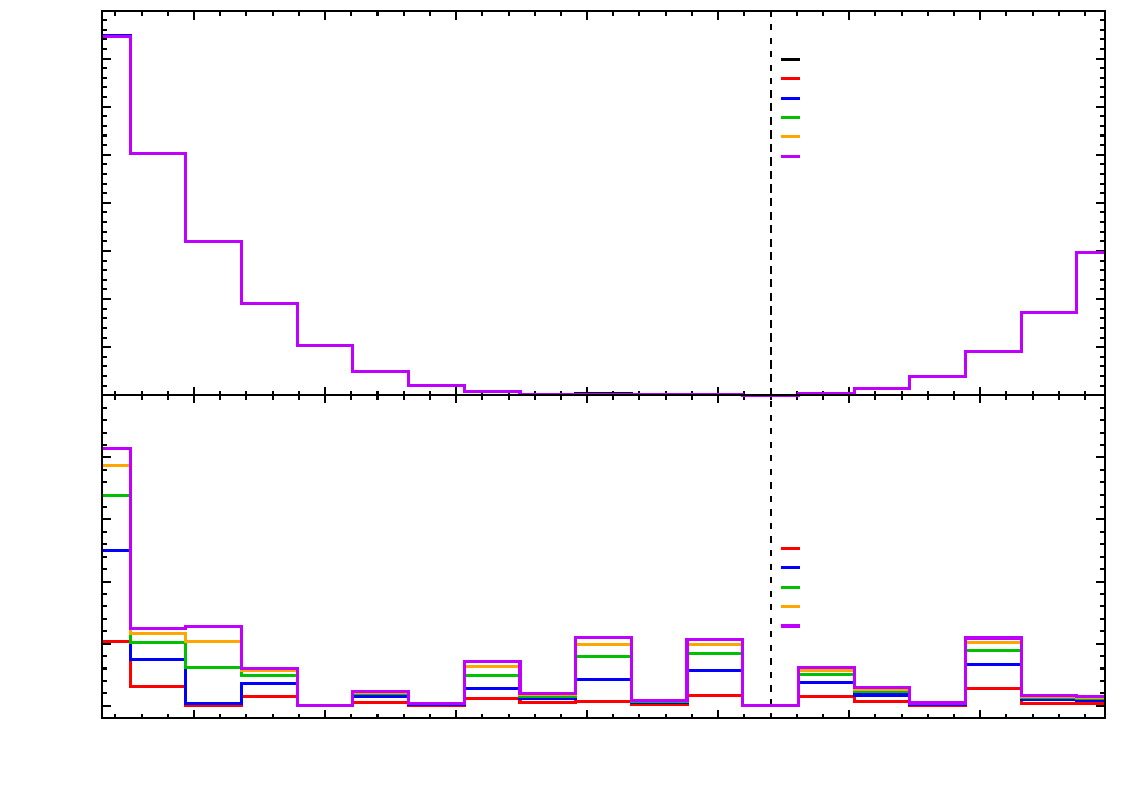
\includegraphics{nuenorm_anti_chi2_S23}}%
    \gplfronttext
  \end{picture}%
\endgroup
}
	\caption[$\chi^2$ profiles for $\Delta m_{32}^2$, $\sin^2 2\theta_{13}$, and $\sin\theta_{23}$ with a simplified systematic model]%
		{The top panels of each figure show the $\chi^2$ profile for %
		$\Delta m_{32}^2$ (top), $\sin^2 2\theta_{13}$ (middle), and $\sin\theta_{23}$ 
		for correlated (left) and anticorrelated (right) systematics. 
		The degeneracy in the $\chi^2$ for $\Delta m_{32}^2$ is slightly with anticorrelated systematics, %
		whereas the opposite is true for the angles $\theta_{23}$ and $\theta_{13}$, %
		even though the latter shows variation not only for correlated, but also for anticorrelated systematics.
		The bottom panels show instead the difference between the profiles at different error magnitudes and %
		the curve computed without systematic uncertainties (black).
		The dashed lines show the position of the best fit value, which is always at the nominal Asimov~A value.}
	\label{fig:nuenorm_mass_angles}
\end{figure}

\begin{figure}
	\centering
	\resizebox{0.49\linewidth}{!}{% GNUPLOT: LaTeX picture with Postscript
\begingroup
  \makeatletter
  \providecommand\color[2][]{%
    \GenericError{(gnuplot) \space\space\space\@spaces}{%
      Package color not loaded in conjunction with
      terminal option `colourtext'%
    }{See the gnuplot documentation for explanation.%
    }{Either use 'blacktext' in gnuplot or load the package
      color.sty in LaTeX.}%
    \renewcommand\color[2][]{}%
  }%
  \providecommand\includegraphics[2][]{%
    \GenericError{(gnuplot) \space\space\space\@spaces}{%
      Package graphicx or graphics not loaded%
    }{See the gnuplot documentation for explanation.%
    }{The gnuplot epslatex terminal needs graphicx.sty or graphics.sty.}%
    \renewcommand\includegraphics[2][]{}%
  }%
  \providecommand\rotatebox[2]{#2}%
  \@ifundefined{ifGPcolor}{%
    \newif\ifGPcolor
    \GPcolortrue
  }{}%
  \@ifundefined{ifGPblacktext}{%
    \newif\ifGPblacktext
    \GPblacktexttrue
  }{}%
  % define a \g@addto@macro without @ in the name:
  \let\gplgaddtomacro\g@addto@macro
  % define empty templates for all commands taking text:
  \gdef\gplbacktext{}%
  \gdef\gplfronttext{}%
  \makeatother
  \ifGPblacktext
    % no textcolor at all
    \def\colorrgb#1{}%
    \def\colorgray#1{}%
  \else
    % gray or color?
    \ifGPcolor
      \def\colorrgb#1{\color[rgb]{#1}}%
      \def\colorgray#1{\color[gray]{#1}}%
      \expandafter\def\csname LTw\endcsname{\color{white}}%
      \expandafter\def\csname LTb\endcsname{\color{black}}%
      \expandafter\def\csname LTa\endcsname{\color{black}}%
      \expandafter\def\csname LT0\endcsname{\color[rgb]{1,0,0}}%
      \expandafter\def\csname LT1\endcsname{\color[rgb]{0,1,0}}%
      \expandafter\def\csname LT2\endcsname{\color[rgb]{0,0,1}}%
      \expandafter\def\csname LT3\endcsname{\color[rgb]{1,0,1}}%
      \expandafter\def\csname LT4\endcsname{\color[rgb]{0,1,1}}%
      \expandafter\def\csname LT5\endcsname{\color[rgb]{1,1,0}}%
      \expandafter\def\csname LT6\endcsname{\color[rgb]{0,0,0}}%
      \expandafter\def\csname LT7\endcsname{\color[rgb]{1,0.3,0}}%
      \expandafter\def\csname LT8\endcsname{\color[rgb]{0.5,0.5,0.5}}%
    \else
      % gray
      \def\colorrgb#1{\color{black}}%
      \def\colorgray#1{\color[gray]{#1}}%
      \expandafter\def\csname LTw\endcsname{\color{white}}%
      \expandafter\def\csname LTb\endcsname{\color{black}}%
      \expandafter\def\csname LTa\endcsname{\color{black}}%
      \expandafter\def\csname LT0\endcsname{\color{black}}%
      \expandafter\def\csname LT1\endcsname{\color{black}}%
      \expandafter\def\csname LT2\endcsname{\color{black}}%
      \expandafter\def\csname LT3\endcsname{\color{black}}%
      \expandafter\def\csname LT4\endcsname{\color{black}}%
      \expandafter\def\csname LT5\endcsname{\color{black}}%
      \expandafter\def\csname LT6\endcsname{\color{black}}%
      \expandafter\def\csname LT7\endcsname{\color{black}}%
      \expandafter\def\csname LT8\endcsname{\color{black}}%
    \fi
  \fi
    \setlength{\unitlength}{0.0500bp}%
    \ifx\gptboxheight\undefined%
      \newlength{\gptboxheight}%
      \newlength{\gptboxwidth}%
      \newsavebox{\gptboxtext}%
    \fi%
    \setlength{\fboxrule}{0.5pt}%
    \setlength{\fboxsep}{1pt}%
\begin{picture}(7200.00,5760.00)%
    \gplgaddtomacro\gplbacktext{%
      \csname LTb\endcsname%%
      \put(747,927){\makebox(0,0)[r]{\strut{}2.47}}%
      \csname LTb\endcsname%%
      \put(747,1480){\makebox(0,0)[r]{\strut{}2.48}}%
      \csname LTb\endcsname%%
      \put(747,2033){\makebox(0,0)[r]{\strut{}2.49}}%
      \csname LTb\endcsname%%
      \put(747,2586){\makebox(0,0)[r]{\strut{}2.5}}%
      \csname LTb\endcsname%%
      \put(747,3139){\makebox(0,0)[r]{\strut{}2.51}}%
      \csname LTb\endcsname%%
      \put(747,3692){\makebox(0,0)[r]{\strut{}2.52}}%
      \csname LTb\endcsname%%
      \put(747,4246){\makebox(0,0)[r]{\strut{}2.53}}%
      \csname LTb\endcsname%%
      \put(747,4799){\makebox(0,0)[r]{\strut{}2.54}}%
      \csname LTb\endcsname%%
      \put(747,5352){\makebox(0,0)[r]{\strut{}2.55}}%
      \csname LTb\endcsname%%
      \put(1402,409){\makebox(0,0){\strut{}0.44}}%
      \csname LTb\endcsname%%
      \put(2192,409){\makebox(0,0){\strut{}0.46}}%
      \csname LTb\endcsname%%
      \put(2982,409){\makebox(0,0){\strut{}0.48}}%
      \csname LTb\endcsname%%
      \put(3772,409){\makebox(0,0){\strut{}0.5}}%
      \csname LTb\endcsname%%
      \put(4562,409){\makebox(0,0){\strut{}0.52}}%
      \csname LTb\endcsname%%
      \put(5352,409){\makebox(0,0){\strut{}0.54}}%
      \csname LTb\endcsname%%
      \put(6142,409){\makebox(0,0){\strut{}0.56}}%
      \csname LTb\endcsname%%
      \put(4915,3121){\makebox(0,0)[l]{\strut{}}}%
    }%
    \gplgaddtomacro\gplfronttext{%
      \csname LTb\endcsname%%
      \put(153,3084){\rotatebox{-270}{\makebox(0,0){\strut{}$\Delta m_{32}^2 / 10^{-3}$}}}%
      \csname LTb\endcsname%%
      \put(3871,130){\makebox(0,0){\strut{}$\sin^2 \theta_{23}$}}%
      \csname LTb\endcsname%%
      \put(6360,5406){\makebox(0,0)[r]{\strut{}No syst}}%
      \csname LTb\endcsname%%
      \put(6360,5220){\makebox(0,0)[r]{\strut{}1\,\%}}%
      \csname LTb\endcsname%%
      \put(6360,5034){\makebox(0,0)[r]{\strut{}2\,\%}}%
      \csname LTb\endcsname%%
      \put(6360,4848){\makebox(0,0)[r]{\strut{}3\,\%}}%
      \csname LTb\endcsname%%
      \put(6360,4662){\makebox(0,0)[r]{\strut{}4\,\%}}%
      \csname LTb\endcsname%%
      \put(6360,4476){\makebox(0,0)[r]{\strut{}5\,\%}}%
    }%
    \gplbacktext
    \put(0,0){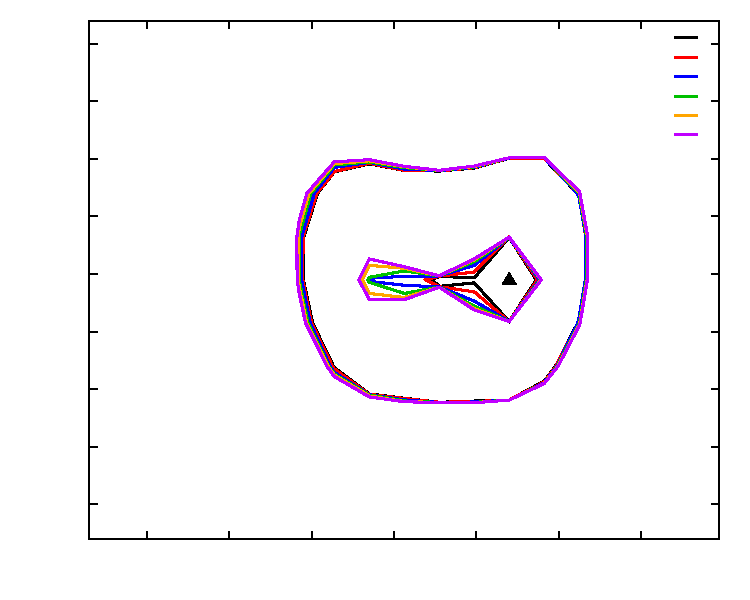
\includegraphics{pics/nuenorm_corr_cont_S23_M23}}%
    \gplfronttext
  \end{picture}%
\endgroup
}	%%%%%%%%%%%this is important
	\resizebox{0.49\linewidth}{!}{% GNUPLOT: LaTeX picture with Postscript
\begingroup
  \makeatletter
  \providecommand\color[2][]{%
    \GenericError{(gnuplot) \space\space\space\@spaces}{%
      Package color not loaded in conjunction with
      terminal option `colourtext'%
    }{See the gnuplot documentation for explanation.%
    }{Either use 'blacktext' in gnuplot or load the package
      color.sty in LaTeX.}%
    \renewcommand\color[2][]{}%
  }%
  \providecommand\includegraphics[2][]{%
    \GenericError{(gnuplot) \space\space\space\@spaces}{%
      Package graphicx or graphics not loaded%
    }{See the gnuplot documentation for explanation.%
    }{The gnuplot epslatex terminal needs graphicx.sty or graphics.sty.}%
    \renewcommand\includegraphics[2][]{}%
  }%
  \providecommand\rotatebox[2]{#2}%
  \@ifundefined{ifGPcolor}{%
    \newif\ifGPcolor
    \GPcolortrue
  }{}%
  \@ifundefined{ifGPblacktext}{%
    \newif\ifGPblacktext
    \GPblacktexttrue
  }{}%
  % define a \g@addto@macro without @ in the name:
  \let\gplgaddtomacro\g@addto@macro
  % define empty templates for all commands taking text:
  \gdef\gplbacktext{}%
  \gdef\gplfronttext{}%
  \makeatother
  \ifGPblacktext
    % no textcolor at all
    \def\colorrgb#1{}%
    \def\colorgray#1{}%
  \else
    % gray or color?
    \ifGPcolor
      \def\colorrgb#1{\color[rgb]{#1}}%
      \def\colorgray#1{\color[gray]{#1}}%
      \expandafter\def\csname LTw\endcsname{\color{white}}%
      \expandafter\def\csname LTb\endcsname{\color{black}}%
      \expandafter\def\csname LTa\endcsname{\color{black}}%
      \expandafter\def\csname LT0\endcsname{\color[rgb]{1,0,0}}%
      \expandafter\def\csname LT1\endcsname{\color[rgb]{0,1,0}}%
      \expandafter\def\csname LT2\endcsname{\color[rgb]{0,0,1}}%
      \expandafter\def\csname LT3\endcsname{\color[rgb]{1,0,1}}%
      \expandafter\def\csname LT4\endcsname{\color[rgb]{0,1,1}}%
      \expandafter\def\csname LT5\endcsname{\color[rgb]{1,1,0}}%
      \expandafter\def\csname LT6\endcsname{\color[rgb]{0,0,0}}%
      \expandafter\def\csname LT7\endcsname{\color[rgb]{1,0.3,0}}%
      \expandafter\def\csname LT8\endcsname{\color[rgb]{0.5,0.5,0.5}}%
    \else
      % gray
      \def\colorrgb#1{\color{black}}%
      \def\colorgray#1{\color[gray]{#1}}%
      \expandafter\def\csname LTw\endcsname{\color{white}}%
      \expandafter\def\csname LTb\endcsname{\color{black}}%
      \expandafter\def\csname LTa\endcsname{\color{black}}%
      \expandafter\def\csname LT0\endcsname{\color{black}}%
      \expandafter\def\csname LT1\endcsname{\color{black}}%
      \expandafter\def\csname LT2\endcsname{\color{black}}%
      \expandafter\def\csname LT3\endcsname{\color{black}}%
      \expandafter\def\csname LT4\endcsname{\color{black}}%
      \expandafter\def\csname LT5\endcsname{\color{black}}%
      \expandafter\def\csname LT6\endcsname{\color{black}}%
      \expandafter\def\csname LT7\endcsname{\color{black}}%
      \expandafter\def\csname LT8\endcsname{\color{black}}%
    \fi
  \fi
    \setlength{\unitlength}{0.0500bp}%
    \ifx\gptboxheight\undefined%
      \newlength{\gptboxheight}%
      \newlength{\gptboxwidth}%
      \newsavebox{\gptboxtext}%
    \fi%
    \setlength{\fboxrule}{0.5pt}%
    \setlength{\fboxsep}{1pt}%
\begin{picture}(10800.00,7560.00)%
    \gplgaddtomacro\gplbacktext{%
      \csname LTb\endcsname%%
      \put(747,1047){\makebox(0,0)[r]{\strut{}2.47}}%
      \csname LTb\endcsname%%
      \put(747,1800){\makebox(0,0)[r]{\strut{}2.48}}%
      \csname LTb\endcsname%%
      \put(747,2553){\makebox(0,0)[r]{\strut{}2.49}}%
      \csname LTb\endcsname%%
      \put(747,3306){\makebox(0,0)[r]{\strut{}2.5}}%
      \csname LTb\endcsname%%
      \put(747,4059){\makebox(0,0)[r]{\strut{}2.51}}%
      \csname LTb\endcsname%%
      \put(747,4812){\makebox(0,0)[r]{\strut{}2.52}}%
      \csname LTb\endcsname%%
      \put(747,5566){\makebox(0,0)[r]{\strut{}2.53}}%
      \csname LTb\endcsname%%
      \put(747,6319){\makebox(0,0)[r]{\strut{}2.54}}%
      \csname LTb\endcsname%%
      \put(747,7072){\makebox(0,0)[r]{\strut{}2.55}}%
      \csname LTb\endcsname%%
      \put(1731,409){\makebox(0,0){\strut{}0.44}}%
      \csname LTb\endcsname%%
      \put(2992,409){\makebox(0,0){\strut{}0.46}}%
      \csname LTb\endcsname%%
      \put(4253,409){\makebox(0,0){\strut{}0.48}}%
      \csname LTb\endcsname%%
      \put(5513,409){\makebox(0,0){\strut{}0.5}}%
      \csname LTb\endcsname%%
      \put(6774,409){\makebox(0,0){\strut{}0.52}}%
      \csname LTb\endcsname%%
      \put(8035,409){\makebox(0,0){\strut{}0.54}}%
      \csname LTb\endcsname%%
      \put(9295,409){\makebox(0,0){\strut{}0.56}}%
      \csname LTb\endcsname%%
      \put(7315,4021){\makebox(0,0)[l]{\strut{}}}%
    }%
    \gplgaddtomacro\gplfronttext{%
      \csname LTb\endcsname%%
      \put(153,3984){\rotatebox{-270}{\makebox(0,0){\strut{}$\Delta m_{32}^2 / 10^{-3}$}}}%
      \csname LTb\endcsname%%
      \put(5671,130){\makebox(0,0){\strut{}$\sin^2 \theta_{23}$}}%
      \csname LTb\endcsname%%
      \put(9705,7206){\makebox(0,0)[r]{\strut{}No syst}}%
      \csname LTb\endcsname%%
      \put(9705,7020){\makebox(0,0)[r]{\strut{}$1\%$}}%
      \csname LTb\endcsname%%
      \put(9705,6834){\makebox(0,0)[r]{\strut{}$2\%$}}%
      \csname LTb\endcsname%%
      \put(9705,6648){\makebox(0,0)[r]{\strut{}$3\%$}}%
      \csname LTb\endcsname%%
      \put(9705,6462){\makebox(0,0)[r]{\strut{}$4\%$}}%
      \csname LTb\endcsname%%
      \put(9705,6276){\makebox(0,0)[r]{\strut{}$5\%$}}%
    }%
    \gplbacktext
    \put(0,0){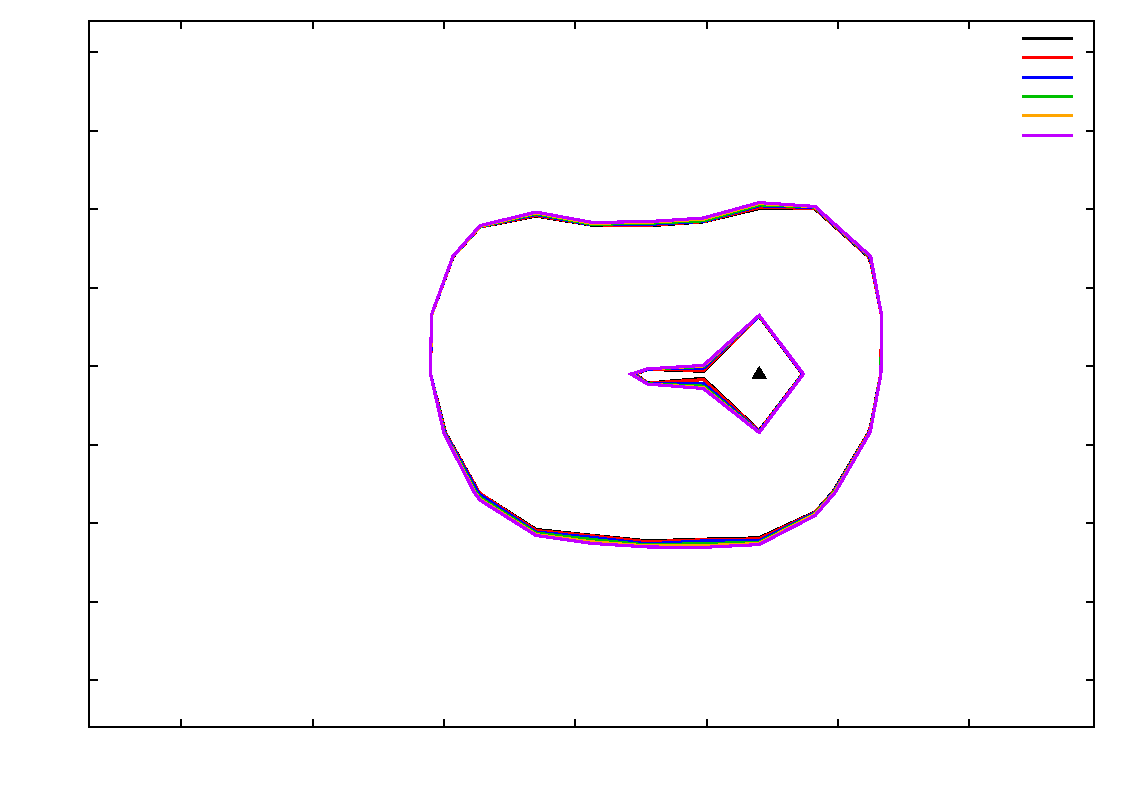
\includegraphics{nuenorm_anti_cont_S23_M23}}%
    \gplfronttext
  \end{picture}%
\endgroup
}
	\resizebox{0.49\linewidth}{!}{% GNUPLOT: LaTeX picture with Postscript
\begingroup
  \makeatletter
  \providecommand\color[2][]{%
    \GenericError{(gnuplot) \space\space\space\@spaces}{%
      Package color not loaded in conjunction with
      terminal option `colourtext'%
    }{See the gnuplot documentation for explanation.%
    }{Either use 'blacktext' in gnuplot or load the package
      color.sty in LaTeX.}%
    \renewcommand\color[2][]{}%
  }%
  \providecommand\includegraphics[2][]{%
    \GenericError{(gnuplot) \space\space\space\@spaces}{%
      Package graphicx or graphics not loaded%
    }{See the gnuplot documentation for explanation.%
    }{The gnuplot epslatex terminal needs graphicx.sty or graphics.sty.}%
    \renewcommand\includegraphics[2][]{}%
  }%
  \providecommand\rotatebox[2]{#2}%
  \@ifundefined{ifGPcolor}{%
    \newif\ifGPcolor
    \GPcolortrue
  }{}%
  \@ifundefined{ifGPblacktext}{%
    \newif\ifGPblacktext
    \GPblacktexttrue
  }{}%
  % define a \g@addto@macro without @ in the name:
  \let\gplgaddtomacro\g@addto@macro
  % define empty templates for all commands taking text:
  \gdef\gplbacktext{}%
  \gdef\gplfronttext{}%
  \makeatother
  \ifGPblacktext
    % no textcolor at all
    \def\colorrgb#1{}%
    \def\colorgray#1{}%
  \else
    % gray or color?
    \ifGPcolor
      \def\colorrgb#1{\color[rgb]{#1}}%
      \def\colorgray#1{\color[gray]{#1}}%
      \expandafter\def\csname LTw\endcsname{\color{white}}%
      \expandafter\def\csname LTb\endcsname{\color{black}}%
      \expandafter\def\csname LTa\endcsname{\color{black}}%
      \expandafter\def\csname LT0\endcsname{\color[rgb]{1,0,0}}%
      \expandafter\def\csname LT1\endcsname{\color[rgb]{0,1,0}}%
      \expandafter\def\csname LT2\endcsname{\color[rgb]{0,0,1}}%
      \expandafter\def\csname LT3\endcsname{\color[rgb]{1,0,1}}%
      \expandafter\def\csname LT4\endcsname{\color[rgb]{0,1,1}}%
      \expandafter\def\csname LT5\endcsname{\color[rgb]{1,1,0}}%
      \expandafter\def\csname LT6\endcsname{\color[rgb]{0,0,0}}%
      \expandafter\def\csname LT7\endcsname{\color[rgb]{1,0.3,0}}%
      \expandafter\def\csname LT8\endcsname{\color[rgb]{0.5,0.5,0.5}}%
    \else
      % gray
      \def\colorrgb#1{\color{black}}%
      \def\colorgray#1{\color[gray]{#1}}%
      \expandafter\def\csname LTw\endcsname{\color{white}}%
      \expandafter\def\csname LTb\endcsname{\color{black}}%
      \expandafter\def\csname LTa\endcsname{\color{black}}%
      \expandafter\def\csname LT0\endcsname{\color{black}}%
      \expandafter\def\csname LT1\endcsname{\color{black}}%
      \expandafter\def\csname LT2\endcsname{\color{black}}%
      \expandafter\def\csname LT3\endcsname{\color{black}}%
      \expandafter\def\csname LT4\endcsname{\color{black}}%
      \expandafter\def\csname LT5\endcsname{\color{black}}%
      \expandafter\def\csname LT6\endcsname{\color{black}}%
      \expandafter\def\csname LT7\endcsname{\color{black}}%
      \expandafter\def\csname LT8\endcsname{\color{black}}%
    \fi
  \fi
    \setlength{\unitlength}{0.0500bp}%
    \ifx\gptboxheight\undefined%
      \newlength{\gptboxheight}%
      \newlength{\gptboxwidth}%
      \newsavebox{\gptboxtext}%
    \fi%
    \setlength{\fboxrule}{0.5pt}%
    \setlength{\fboxsep}{1pt}%
\begin{picture}(10800.00,7560.00)%
    \gplgaddtomacro\gplbacktext{%
      \csname LTb\endcsname%%
      \put(870,680){\makebox(0,0)[r]{\strut{}-1}}%
      \csname LTb\endcsname%%
      \put(870,1123){\makebox(0,0)[r]{\strut{}0}}%
      \csname LTb\endcsname%%
      \put(870,1566){\makebox(0,0)[r]{\strut{}1}}%
      \csname LTb\endcsname%%
      \put(870,2009){\makebox(0,0)[r]{\strut{}2}}%
      \csname LTb\endcsname%%
      \put(870,2451){\makebox(0,0)[r]{\strut{}3}}%
      \csname LTb\endcsname%%
      \put(870,2894){\makebox(0,0)[r]{\strut{}4}}%
      \csname LTb\endcsname%%
      \put(870,3337){\makebox(0,0)[r]{\strut{}5}}%
      \csname LTb\endcsname%%
      \put(972,494){\makebox(0,0){\strut{}-1.00$\pi$}}%
      \csname LTb\endcsname%%
      \put(1934,494){\makebox(0,0){\strut{}-0.80$\pi$}}%
      \csname LTb\endcsname%%
      \put(2897,494){\makebox(0,0){\strut{}-0.60$\pi$}}%
      \csname LTb\endcsname%%
      \put(3859,494){\makebox(0,0){\strut{}-0.40$\pi$}}%
      \csname LTb\endcsname%%
      \put(4821,494){\makebox(0,0){\strut{}-0.20$\pi$}}%
      \csname LTb\endcsname%%
      \put(5784,494){\makebox(0,0){\strut{}0.00$\pi$}}%
      \csname LTb\endcsname%%
      \put(6746,494){\makebox(0,0){\strut{}0.20$\pi$}}%
      \csname LTb\endcsname%%
      \put(7708,494){\makebox(0,0){\strut{}0.40$\pi$}}%
      \csname LTb\endcsname%%
      \put(8670,494){\makebox(0,0){\strut{}0.60$\pi$}}%
      \csname LTb\endcsname%%
      \put(9633,494){\makebox(0,0){\strut{}0.80$\pi$}}%
      \csname LTb\endcsname%%
      \put(10595,494){\makebox(0,0){\strut{}1.00$\pi$}}%
    }%
    \gplgaddtomacro\gplfronttext{%
      \csname LTb\endcsname%%
      \put(480,2230){\rotatebox{-270}{\makebox(0,0){\strut{}$\Delta \chi^2 - \Delta \chi^2_0$}}}%
      \csname LTb\endcsname%%
      \put(5783,215){\makebox(0,0){\strut{}$\delta_\text{CP}$}}%
      \csname LTb\endcsname%%
      \put(4231,2358){\makebox(0,0){\strut{}Difference}}%
      \csname LTb\endcsname%%
      \put(3758,2172){\makebox(0,0)[l]{\strut{}$1\%$}}%
      \csname LTb\endcsname%%
      \put(3758,1986){\makebox(0,0)[l]{\strut{}$2\%$}}%
      \csname LTb\endcsname%%
      \put(3758,1800){\makebox(0,0)[l]{\strut{}$3\%$}}%
      \csname LTb\endcsname%%
      \put(3758,1614){\makebox(0,0)[l]{\strut{}$4\%$}}%
      \csname LTb\endcsname%%
      \put(3758,1428){\makebox(0,0)[l]{\strut{}$5\%$}}%
    }%
    \gplgaddtomacro\gplbacktext{%
      \csname LTb\endcsname%%
      \put(870,3780){\makebox(0,0)[r]{\strut{}0}}%
      \csname LTb\endcsname%%
      \put(870,4149){\makebox(0,0)[r]{\strut{}50}}%
      \csname LTb\endcsname%%
      \put(870,4517){\makebox(0,0)[r]{\strut{}100}}%
      \csname LTb\endcsname%%
      \put(870,4886){\makebox(0,0)[r]{\strut{}150}}%
      \csname LTb\endcsname%%
      \put(870,5254){\makebox(0,0)[r]{\strut{}200}}%
      \csname LTb\endcsname%%
      \put(870,5623){\makebox(0,0)[r]{\strut{}250}}%
      \csname LTb\endcsname%%
      \put(870,5992){\makebox(0,0)[r]{\strut{}300}}%
      \csname LTb\endcsname%%
      \put(870,6360){\makebox(0,0)[r]{\strut{}350}}%
      \csname LTb\endcsname%%
      \put(870,6729){\makebox(0,0)[r]{\strut{}400}}%
      \csname LTb\endcsname%%
      \put(870,7097){\makebox(0,0)[r]{\strut{}450}}%
      \csname LTb\endcsname%%
      \put(870,7466){\makebox(0,0)[r]{\strut{}500}}%
      \csname LTb\endcsname%%
      \put(972,3594){\makebox(0,0){\strut{}}}%
      \csname LTb\endcsname%%
      \put(1934,3594){\makebox(0,0){\strut{}}}%
      \csname LTb\endcsname%%
      \put(2897,3594){\makebox(0,0){\strut{}}}%
      \csname LTb\endcsname%%
      \put(3859,3594){\makebox(0,0){\strut{}}}%
      \csname LTb\endcsname%%
      \put(4821,3594){\makebox(0,0){\strut{}}}%
      \csname LTb\endcsname%%
      \put(5784,3594){\makebox(0,0){\strut{}}}%
      \csname LTb\endcsname%%
      \put(6746,3594){\makebox(0,0){\strut{}}}%
      \csname LTb\endcsname%%
      \put(7708,3594){\makebox(0,0){\strut{}}}%
      \csname LTb\endcsname%%
      \put(8670,3594){\makebox(0,0){\strut{}}}%
      \csname LTb\endcsname%%
      \put(9633,3594){\makebox(0,0){\strut{}}}%
      \csname LTb\endcsname%%
      \put(10595,3594){\makebox(0,0){\strut{}}}%
    }%
    \gplgaddtomacro\gplfronttext{%
      \csname LTb\endcsname%%
      \put(378,5623){\rotatebox{-270}{\makebox(0,0){\strut{}$\Delta \chi^2$}}}%
      \csname LTb\endcsname%%
      \put(5783,3538){\makebox(0,0){\strut{}}}%
      \csname LTb\endcsname%%
      \put(4231,7004){\makebox(0,0){\strut{}}}%
      \csname LTb\endcsname%%
      \put(3758,7004){\makebox(0,0)[l]{\strut{}No syst}}%
      \csname LTb\endcsname%%
      \put(3758,6818){\makebox(0,0)[l]{\strut{}$1\%$}}%
      \csname LTb\endcsname%%
      \put(3758,6632){\makebox(0,0)[l]{\strut{}$2\%$}}%
      \csname LTb\endcsname%%
      \put(3758,6446){\makebox(0,0)[l]{\strut{}$3\%$}}%
      \csname LTb\endcsname%%
      \put(3758,6260){\makebox(0,0)[l]{\strut{}$4\%$}}%
      \csname LTb\endcsname%%
      \put(3758,6074){\makebox(0,0)[l]{\strut{}$5\%$}}%
    }%
    \gplbacktext
    \put(0,0){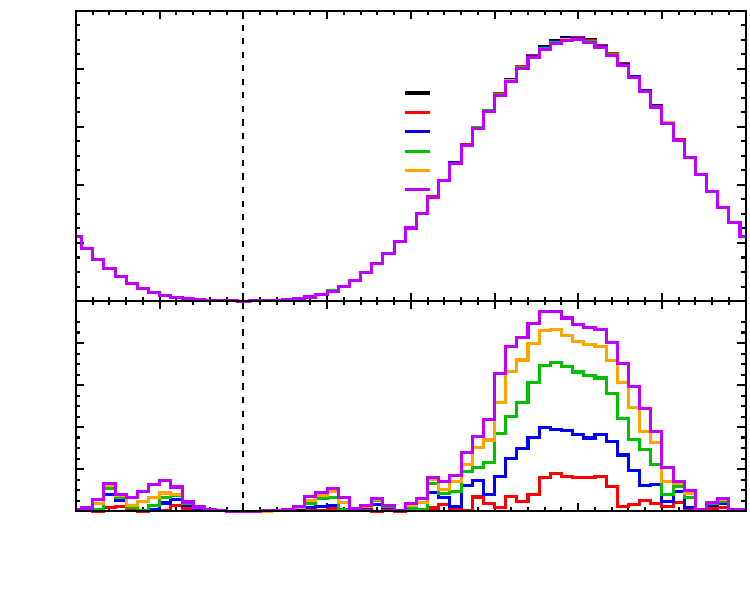
\includegraphics{pics/nuenorm_corr_chi2_dCP}}%
    \gplfronttext
  \end{picture}%
\endgroup
}
	\resizebox{0.49\linewidth}{!}{% GNUPLOT: LaTeX picture with Postscript
\begingroup
  \makeatletter
  \providecommand\color[2][]{%
    \GenericError{(gnuplot) \space\space\space\@spaces}{%
      Package color not loaded in conjunction with
      terminal option `colourtext'%
    }{See the gnuplot documentation for explanation.%
    }{Either use 'blacktext' in gnuplot or load the package
      color.sty in LaTeX.}%
    \renewcommand\color[2][]{}%
  }%
  \providecommand\includegraphics[2][]{%
    \GenericError{(gnuplot) \space\space\space\@spaces}{%
      Package graphicx or graphics not loaded%
    }{See the gnuplot documentation for explanation.%
    }{The gnuplot epslatex terminal needs graphicx.sty or graphics.sty.}%
    \renewcommand\includegraphics[2][]{}%
  }%
  \providecommand\rotatebox[2]{#2}%
  \@ifundefined{ifGPcolor}{%
    \newif\ifGPcolor
    \GPcolortrue
  }{}%
  \@ifundefined{ifGPblacktext}{%
    \newif\ifGPblacktext
    \GPblacktexttrue
  }{}%
  % define a \g@addto@macro without @ in the name:
  \let\gplgaddtomacro\g@addto@macro
  % define empty templates for all commands taking text:
  \gdef\gplbacktext{}%
  \gdef\gplfronttext{}%
  \makeatother
  \ifGPblacktext
    % no textcolor at all
    \def\colorrgb#1{}%
    \def\colorgray#1{}%
  \else
    % gray or color?
    \ifGPcolor
      \def\colorrgb#1{\color[rgb]{#1}}%
      \def\colorgray#1{\color[gray]{#1}}%
      \expandafter\def\csname LTw\endcsname{\color{white}}%
      \expandafter\def\csname LTb\endcsname{\color{black}}%
      \expandafter\def\csname LTa\endcsname{\color{black}}%
      \expandafter\def\csname LT0\endcsname{\color[rgb]{1,0,0}}%
      \expandafter\def\csname LT1\endcsname{\color[rgb]{0,1,0}}%
      \expandafter\def\csname LT2\endcsname{\color[rgb]{0,0,1}}%
      \expandafter\def\csname LT3\endcsname{\color[rgb]{1,0,1}}%
      \expandafter\def\csname LT4\endcsname{\color[rgb]{0,1,1}}%
      \expandafter\def\csname LT5\endcsname{\color[rgb]{1,1,0}}%
      \expandafter\def\csname LT6\endcsname{\color[rgb]{0,0,0}}%
      \expandafter\def\csname LT7\endcsname{\color[rgb]{1,0.3,0}}%
      \expandafter\def\csname LT8\endcsname{\color[rgb]{0.5,0.5,0.5}}%
    \else
      % gray
      \def\colorrgb#1{\color{black}}%
      \def\colorgray#1{\color[gray]{#1}}%
      \expandafter\def\csname LTw\endcsname{\color{white}}%
      \expandafter\def\csname LTb\endcsname{\color{black}}%
      \expandafter\def\csname LTa\endcsname{\color{black}}%
      \expandafter\def\csname LT0\endcsname{\color{black}}%
      \expandafter\def\csname LT1\endcsname{\color{black}}%
      \expandafter\def\csname LT2\endcsname{\color{black}}%
      \expandafter\def\csname LT3\endcsname{\color{black}}%
      \expandafter\def\csname LT4\endcsname{\color{black}}%
      \expandafter\def\csname LT5\endcsname{\color{black}}%
      \expandafter\def\csname LT6\endcsname{\color{black}}%
      \expandafter\def\csname LT7\endcsname{\color{black}}%
      \expandafter\def\csname LT8\endcsname{\color{black}}%
    \fi
  \fi
    \setlength{\unitlength}{0.0500bp}%
    \ifx\gptboxheight\undefined%
      \newlength{\gptboxheight}%
      \newlength{\gptboxwidth}%
      \newsavebox{\gptboxtext}%
    \fi%
    \setlength{\fboxrule}{0.5pt}%
    \setlength{\fboxsep}{1pt}%
\begin{picture}(7200.00,5760.00)%
    \gplgaddtomacro\gplbacktext{%
      \csname LTb\endcsname%%
      \put(618,864){\makebox(0,0)[r]{\strut{}0}}%
      \csname LTb\endcsname%%
      \put(618,1368){\makebox(0,0)[r]{\strut{}100}}%
      \csname LTb\endcsname%%
      \put(618,1872){\makebox(0,0)[r]{\strut{}200}}%
      \csname LTb\endcsname%%
      \put(618,2376){\makebox(0,0)[r]{\strut{}300}}%
      \csname LTb\endcsname%%
      \put(720,678){\makebox(0,0){\strut{}-1.00$\pi$}}%
      \csname LTb\endcsname%%
      \put(1524,678){\makebox(0,0){\strut{}-0.75$\pi$}}%
      \csname LTb\endcsname%%
      \put(2327,678){\makebox(0,0){\strut{}-0.50$\pi$}}%
      \csname LTb\endcsname%%
      \put(3131,678){\makebox(0,0){\strut{}-0.25$\pi$}}%
      \csname LTb\endcsname%%
      \put(3934,678){\makebox(0,0){\strut{}0.00$\pi$}}%
      \csname LTb\endcsname%%
      \put(4738,678){\makebox(0,0){\strut{}0.25$\pi$}}%
      \csname LTb\endcsname%%
      \put(5541,678){\makebox(0,0){\strut{}0.50$\pi$}}%
      \csname LTb\endcsname%%
      \put(6345,678){\makebox(0,0){\strut{}0.75$\pi$}}%
      \csname LTb\endcsname%%
      \put(7148,678){\makebox(0,0){\strut{}1.00$\pi$}}%
    }%
    \gplgaddtomacro\gplfronttext{%
      \csname LTb\endcsname%%
      \put(126,1872){\rotatebox{-270}{\makebox(0,0){\strut{}$\Delta \chi^2_\text{No syst} - \Delta \chi^2$}}}%
      \csname LTb\endcsname%%
      \put(3934,399){\makebox(0,0){\strut{}$\delta_\text{CP}$}}%
    }%
    \gplgaddtomacro\gplbacktext{%
      \csname LTb\endcsname%%
      \put(618,2880){\makebox(0,0)[r]{\strut{}0}}%
      \csname LTb\endcsname%%
      \put(618,3437){\makebox(0,0)[r]{\strut{}100}}%
      \csname LTb\endcsname%%
      \put(618,3994){\makebox(0,0)[r]{\strut{}200}}%
      \csname LTb\endcsname%%
      \put(618,4552){\makebox(0,0)[r]{\strut{}300}}%
      \csname LTb\endcsname%%
      \put(618,5109){\makebox(0,0)[r]{\strut{}400}}%
      \csname LTb\endcsname%%
      \put(618,5666){\makebox(0,0)[r]{\strut{}500}}%
      \csname LTb\endcsname%%
      \put(720,2694){\makebox(0,0){\strut{}}}%
      \csname LTb\endcsname%%
      \put(1524,2694){\makebox(0,0){\strut{}}}%
      \csname LTb\endcsname%%
      \put(2327,2694){\makebox(0,0){\strut{}}}%
      \csname LTb\endcsname%%
      \put(3131,2694){\makebox(0,0){\strut{}}}%
      \csname LTb\endcsname%%
      \put(3934,2694){\makebox(0,0){\strut{}}}%
      \csname LTb\endcsname%%
      \put(4738,2694){\makebox(0,0){\strut{}}}%
      \csname LTb\endcsname%%
      \put(5541,2694){\makebox(0,0){\strut{}}}%
      \csname LTb\endcsname%%
      \put(6345,2694){\makebox(0,0){\strut{}}}%
      \csname LTb\endcsname%%
      \put(7148,2694){\makebox(0,0){\strut{}}}%
    }%
    \gplgaddtomacro\gplfronttext{%
      \csname LTb\endcsname%%
      \put(126,4273){\rotatebox{-270}{\makebox(0,0){\strut{}$\Delta \chi^2$}}}%
      \csname LTb\endcsname%%
      \put(3934,2638){\makebox(0,0){\strut{}}}%
      \csname LTb\endcsname%%
      \put(3334,4877){\makebox(0,0){\strut{}}}%
      \csname LTb\endcsname%%
      \put(3782,4877){\makebox(0,0)[r]{\strut{}No syst}}%
      \csname LTb\endcsname%%
      \put(3782,4691){\makebox(0,0)[r]{\strut{}1\,\%}}%
      \csname LTb\endcsname%%
      \put(3782,4505){\makebox(0,0)[r]{\strut{}2\,\%}}%
      \csname LTb\endcsname%%
      \put(3782,4319){\makebox(0,0)[r]{\strut{}3\,\%}}%
      \csname LTb\endcsname%%
      \put(3782,4133){\makebox(0,0)[r]{\strut{}4\,\%}}%
      \csname LTb\endcsname%%
      \put(3782,3947){\makebox(0,0)[r]{\strut{}5\,\%}}%
    }%
    \gplbacktext
    \put(0,0){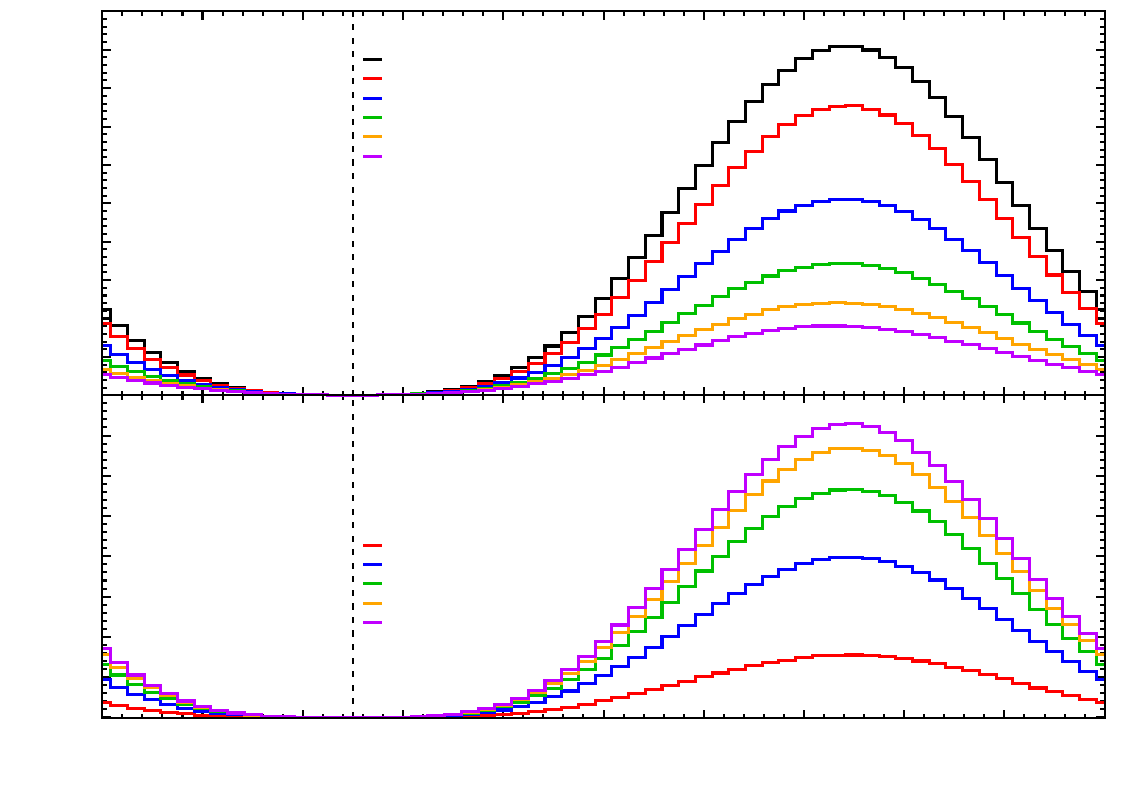
\includegraphics{pics/nuenorm_anti_chi2_dCP}}%
    \gplfronttext
  \end{picture}%
\endgroup
}
	\resizebox{0.49\linewidth}{!}{% GNUPLOT: LaTeX picture with Postscript
\begingroup
  \makeatletter
  \providecommand\color[2][]{%
    \GenericError{(gnuplot) \space\space\space\@spaces}{%
      Package color not loaded in conjunction with
      terminal option `colourtext'%
    }{See the gnuplot documentation for explanation.%
    }{Either use 'blacktext' in gnuplot or load the package
      color.sty in LaTeX.}%
    \renewcommand\color[2][]{}%
  }%
  \providecommand\includegraphics[2][]{%
    \GenericError{(gnuplot) \space\space\space\@spaces}{%
      Package graphicx or graphics not loaded%
    }{See the gnuplot documentation for explanation.%
    }{The gnuplot epslatex terminal needs graphicx.sty or graphics.sty.}%
    \renewcommand\includegraphics[2][]{}%
  }%
  \providecommand\rotatebox[2]{#2}%
  \@ifundefined{ifGPcolor}{%
    \newif\ifGPcolor
    \GPcolortrue
  }{}%
  \@ifundefined{ifGPblacktext}{%
    \newif\ifGPblacktext
    \GPblacktexttrue
  }{}%
  % define a \g@addto@macro without @ in the name:
  \let\gplgaddtomacro\g@addto@macro
  % define empty templates for all commands taking text:
  \gdef\gplbacktext{}%
  \gdef\gplfronttext{}%
  \makeatother
  \ifGPblacktext
    % no textcolor at all
    \def\colorrgb#1{}%
    \def\colorgray#1{}%
  \else
    % gray or color?
    \ifGPcolor
      \def\colorrgb#1{\color[rgb]{#1}}%
      \def\colorgray#1{\color[gray]{#1}}%
      \expandafter\def\csname LTw\endcsname{\color{white}}%
      \expandafter\def\csname LTb\endcsname{\color{black}}%
      \expandafter\def\csname LTa\endcsname{\color{black}}%
      \expandafter\def\csname LT0\endcsname{\color[rgb]{1,0,0}}%
      \expandafter\def\csname LT1\endcsname{\color[rgb]{0,1,0}}%
      \expandafter\def\csname LT2\endcsname{\color[rgb]{0,0,1}}%
      \expandafter\def\csname LT3\endcsname{\color[rgb]{1,0,1}}%
      \expandafter\def\csname LT4\endcsname{\color[rgb]{0,1,1}}%
      \expandafter\def\csname LT5\endcsname{\color[rgb]{1,1,0}}%
      \expandafter\def\csname LT6\endcsname{\color[rgb]{0,0,0}}%
      \expandafter\def\csname LT7\endcsname{\color[rgb]{1,0.3,0}}%
      \expandafter\def\csname LT8\endcsname{\color[rgb]{0.5,0.5,0.5}}%
    \else
      % gray
      \def\colorrgb#1{\color{black}}%
      \def\colorgray#1{\color[gray]{#1}}%
      \expandafter\def\csname LTw\endcsname{\color{white}}%
      \expandafter\def\csname LTb\endcsname{\color{black}}%
      \expandafter\def\csname LTa\endcsname{\color{black}}%
      \expandafter\def\csname LT0\endcsname{\color{black}}%
      \expandafter\def\csname LT1\endcsname{\color{black}}%
      \expandafter\def\csname LT2\endcsname{\color{black}}%
      \expandafter\def\csname LT3\endcsname{\color{black}}%
      \expandafter\def\csname LT4\endcsname{\color{black}}%
      \expandafter\def\csname LT5\endcsname{\color{black}}%
      \expandafter\def\csname LT6\endcsname{\color{black}}%
      \expandafter\def\csname LT7\endcsname{\color{black}}%
      \expandafter\def\csname LT8\endcsname{\color{black}}%
    \fi
  \fi
    \setlength{\unitlength}{0.0500bp}%
    \ifx\gptboxheight\undefined%
      \newlength{\gptboxheight}%
      \newlength{\gptboxwidth}%
      \newsavebox{\gptboxtext}%
    \fi%
    \setlength{\fboxrule}{0.5pt}%
    \setlength{\fboxsep}{1pt}%
\begin{picture}(11520.00,6540.00)%
    \gplgaddtomacro\gplbacktext{%
      \csname LTb\endcsname%%
      \put(543,595){\makebox(0,0)[r]{\strut{}0}}%
      \csname LTb\endcsname%%
      \put(543,1555){\makebox(0,0)[r]{\strut{}2}}%
      \csname LTb\endcsname%%
      \put(543,2514){\makebox(0,0)[r]{\strut{}4}}%
      \csname LTb\endcsname%%
      \put(543,3474){\makebox(0,0)[r]{\strut{}6}}%
      \csname LTb\endcsname%%
      \put(543,4434){\makebox(0,0)[r]{\strut{}8}}%
      \csname LTb\endcsname%%
      \put(543,5393){\makebox(0,0)[r]{\strut{}10}}%
      \csname LTb\endcsname%%
      \put(543,6353){\makebox(0,0)[r]{\strut{}12}}%
      \csname LTb\endcsname%%
      \put(883,409){\makebox(0,0){\strut{}-1.0$\pi$}}%
      \csname LTb\endcsname%%
      \put(2565,409){\makebox(0,0){\strut{}-0.6$\pi$}}%
      \csname LTb\endcsname%%
      \put(4247,409){\makebox(0,0){\strut{}-0.3$\pi$}}%
      \csname LTb\endcsname%%
      \put(5929,409){\makebox(0,0){\strut{}0.0$\pi$}}%
      \csname LTb\endcsname%%
      \put(7611,409){\makebox(0,0){\strut{}0.3$\pi$}}%
      \csname LTb\endcsname%%
      \put(9293,409){\makebox(0,0){\strut{}0.6$\pi$}}%
      \csname LTb\endcsname%%
      \put(10975,409){\makebox(0,0){\strut{}1.0$\pi$}}%
      \csname LTb\endcsname%%
      \put(5929,3234){\makebox(0,0){\strut{}$5 \sigma$}}%
      \csname LTb\endcsname%%
      \put(5929,2274){\makebox(0,0){\strut{}$3 \sigma$}}%
    }%
    \gplgaddtomacro\gplfronttext{%
      \csname LTb\endcsname%%
      \put(153,3474){\rotatebox{-270}{\makebox(0,0){\strut{}$\sigma (\delta_\text{CP})$}}}%
      \csname LTb\endcsname%%
      \put(5929,130){\makebox(0,0){\strut{}$\delta_\text{CP}$}}%
      \csname LTb\endcsname%%
      \put(1178,6186){\makebox(0,0)[l]{\strut{}No syst}}%
      \csname LTb\endcsname%%
      \put(1178,6000){\makebox(0,0)[l]{\strut{}$1\%$}}%
      \csname LTb\endcsname%%
      \put(1178,5814){\makebox(0,0)[l]{\strut{}$2\%$}}%
      \csname LTb\endcsname%%
      \put(1178,5628){\makebox(0,0)[l]{\strut{}$3\%$}}%
      \csname LTb\endcsname%%
      \put(1178,5442){\makebox(0,0)[l]{\strut{}$4\%$}}%
      \csname LTb\endcsname%%
      \put(1178,5256){\makebox(0,0)[l]{\strut{}$5\%$}}%
    }%
    \gplbacktext
    \put(0,0){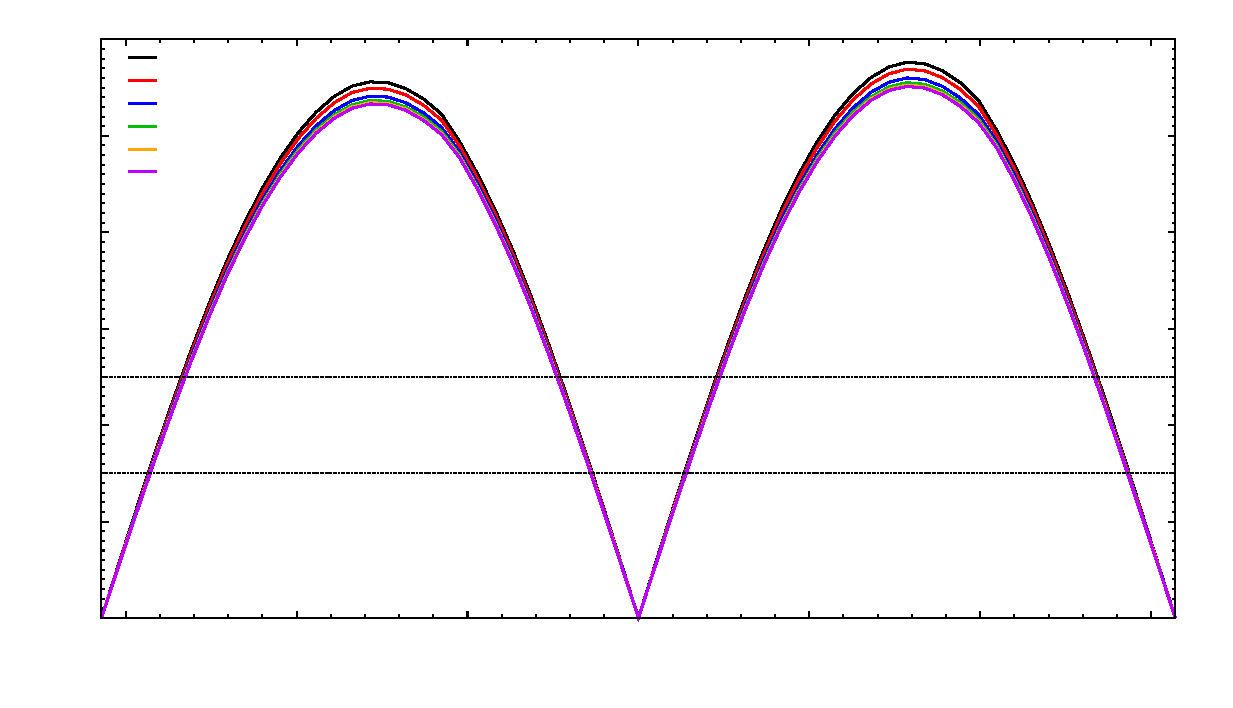
\includegraphics{pics/nuenorm_corr_sensitivity}}%
    \gplfronttext
  \end{picture}%
\endgroup
}
	\resizebox{0.49\linewidth}{!}{% GNUPLOT: LaTeX picture with Postscript
\begingroup
  \makeatletter
  \providecommand\color[2][]{%
    \GenericError{(gnuplot) \space\space\space\@spaces}{%
      Package color not loaded in conjunction with
      terminal option `colourtext'%
    }{See the gnuplot documentation for explanation.%
    }{Either use 'blacktext' in gnuplot or load the package
      color.sty in LaTeX.}%
    \renewcommand\color[2][]{}%
  }%
  \providecommand\includegraphics[2][]{%
    \GenericError{(gnuplot) \space\space\space\@spaces}{%
      Package graphicx or graphics not loaded%
    }{See the gnuplot documentation for explanation.%
    }{The gnuplot epslatex terminal needs graphicx.sty or graphics.sty.}%
    \renewcommand\includegraphics[2][]{}%
  }%
  \providecommand\rotatebox[2]{#2}%
  \@ifundefined{ifGPcolor}{%
    \newif\ifGPcolor
    \GPcolortrue
  }{}%
  \@ifundefined{ifGPblacktext}{%
    \newif\ifGPblacktext
    \GPblacktexttrue
  }{}%
  % define a \g@addto@macro without @ in the name:
  \let\gplgaddtomacro\g@addto@macro
  % define empty templates for all commands taking text:
  \gdef\gplbacktext{}%
  \gdef\gplfronttext{}%
  \makeatother
  \ifGPblacktext
    % no textcolor at all
    \def\colorrgb#1{}%
    \def\colorgray#1{}%
  \else
    % gray or color?
    \ifGPcolor
      \def\colorrgb#1{\color[rgb]{#1}}%
      \def\colorgray#1{\color[gray]{#1}}%
      \expandafter\def\csname LTw\endcsname{\color{white}}%
      \expandafter\def\csname LTb\endcsname{\color{black}}%
      \expandafter\def\csname LTa\endcsname{\color{black}}%
      \expandafter\def\csname LT0\endcsname{\color[rgb]{1,0,0}}%
      \expandafter\def\csname LT1\endcsname{\color[rgb]{0,1,0}}%
      \expandafter\def\csname LT2\endcsname{\color[rgb]{0,0,1}}%
      \expandafter\def\csname LT3\endcsname{\color[rgb]{1,0,1}}%
      \expandafter\def\csname LT4\endcsname{\color[rgb]{0,1,1}}%
      \expandafter\def\csname LT5\endcsname{\color[rgb]{1,1,0}}%
      \expandafter\def\csname LT6\endcsname{\color[rgb]{0,0,0}}%
      \expandafter\def\csname LT7\endcsname{\color[rgb]{1,0.3,0}}%
      \expandafter\def\csname LT8\endcsname{\color[rgb]{0.5,0.5,0.5}}%
    \else
      % gray
      \def\colorrgb#1{\color{black}}%
      \def\colorgray#1{\color[gray]{#1}}%
      \expandafter\def\csname LTw\endcsname{\color{white}}%
      \expandafter\def\csname LTb\endcsname{\color{black}}%
      \expandafter\def\csname LTa\endcsname{\color{black}}%
      \expandafter\def\csname LT0\endcsname{\color{black}}%
      \expandafter\def\csname LT1\endcsname{\color{black}}%
      \expandafter\def\csname LT2\endcsname{\color{black}}%
      \expandafter\def\csname LT3\endcsname{\color{black}}%
      \expandafter\def\csname LT4\endcsname{\color{black}}%
      \expandafter\def\csname LT5\endcsname{\color{black}}%
      \expandafter\def\csname LT6\endcsname{\color{black}}%
      \expandafter\def\csname LT7\endcsname{\color{black}}%
      \expandafter\def\csname LT8\endcsname{\color{black}}%
    \fi
  \fi
    \setlength{\unitlength}{0.0500bp}%
    \ifx\gptboxheight\undefined%
      \newlength{\gptboxheight}%
      \newlength{\gptboxwidth}%
      \newsavebox{\gptboxtext}%
    \fi%
    \setlength{\fboxrule}{0.5pt}%
    \setlength{\fboxsep}{1pt}%
\begin{picture}(7200.00,5040.00)%
    \gplgaddtomacro\gplbacktext{%
      \csname LTb\endcsname%%
      \put(543,595){\makebox(0,0)[r]{\strut{}0}}%
      \csname LTb\endcsname%%
      \put(543,1305){\makebox(0,0)[r]{\strut{}2}}%
      \csname LTb\endcsname%%
      \put(543,2014){\makebox(0,0)[r]{\strut{}4}}%
      \csname LTb\endcsname%%
      \put(543,2724){\makebox(0,0)[r]{\strut{}6}}%
      \csname LTb\endcsname%%
      \put(543,3434){\makebox(0,0)[r]{\strut{}8}}%
      \csname LTb\endcsname%%
      \put(543,4143){\makebox(0,0)[r]{\strut{}10}}%
      \csname LTb\endcsname%%
      \put(543,4853){\makebox(0,0)[r]{\strut{}12}}%
      \csname LTb\endcsname%%
      \put(645,409){\makebox(0,0){\strut{}-1.0$\pi$}}%
      \csname LTb\endcsname%%
      \put(1426,409){\makebox(0,0){\strut{}-0.8$\pi$}}%
      \csname LTb\endcsname%%
      \put(2207,409){\makebox(0,0){\strut{}-0.5$\pi$}}%
      \csname LTb\endcsname%%
      \put(2988,409){\makebox(0,0){\strut{}-0.2$\pi$}}%
      \csname LTb\endcsname%%
      \put(3769,409){\makebox(0,0){\strut{}0.0$\pi$}}%
      \csname LTb\endcsname%%
      \put(4550,409){\makebox(0,0){\strut{}0.2$\pi$}}%
      \csname LTb\endcsname%%
      \put(5331,409){\makebox(0,0){\strut{}0.5$\pi$}}%
      \csname LTb\endcsname%%
      \put(6112,409){\makebox(0,0){\strut{}0.8$\pi$}}%
      \csname LTb\endcsname%%
      \put(6893,409){\makebox(0,0){\strut{}1.0$\pi$}}%
      \csname LTb\endcsname%%
      \put(3769,2547){\makebox(0,0){\strut{}$5 \sigma$}}%
      \csname LTb\endcsname%%
      \put(3769,1837){\makebox(0,0){\strut{}$3 \sigma$}}%
    }%
    \gplgaddtomacro\gplfronttext{%
      \csname LTb\endcsname%%
      \put(153,2724){\rotatebox{-270}{\makebox(0,0){\strut{}$\sigma (\delta_\text{CP})$}}}%
      \csname LTb\endcsname%%
      \put(3769,130){\makebox(0,0){\strut{}$\delta_\text{CP}$}}%
      \csname LTb\endcsname%%
      \put(1178,4686){\makebox(0,0)[l]{\strut{}No syst}}%
      \csname LTb\endcsname%%
      \put(1178,4500){\makebox(0,0)[l]{\strut{}1\,\%}}%
      \csname LTb\endcsname%%
      \put(1178,4314){\makebox(0,0)[l]{\strut{}2\,\%}}%
      \csname LTb\endcsname%%
      \put(1178,4128){\makebox(0,0)[l]{\strut{}3\,\%}}%
      \csname LTb\endcsname%%
      \put(1178,3942){\makebox(0,0)[l]{\strut{}4\,\%}}%
      \csname LTb\endcsname%%
      \put(1178,3756){\makebox(0,0)[l]{\strut{}5\,\%}}%
    }%
    \gplbacktext
    \put(0,0){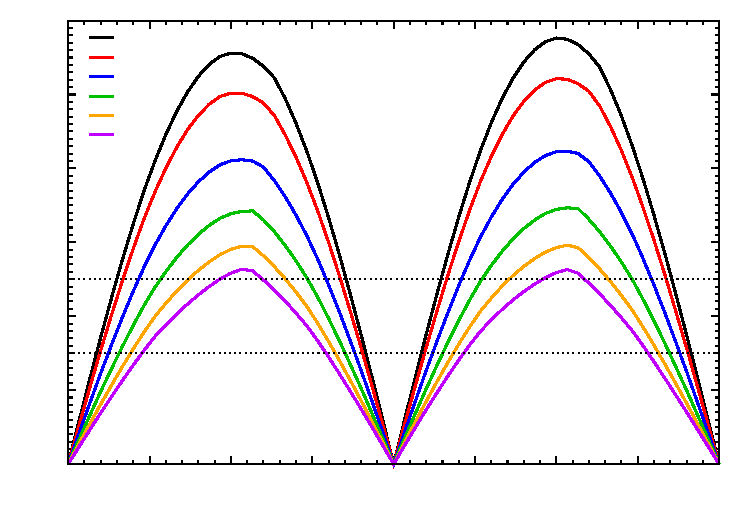
\includegraphics{pics/nuenorm_anti_sensitivity}}%
    \gplfronttext
  \end{picture}%
\endgroup
}
	\caption[Contour lines of $\Delta m_{32}^2$ versus $\sin^2 2\theta_{13}$, $\chi^2$ profiles for $\delta_\text{CP}$, %
		and sensitivity to $\delta_{CP}$$\sin\theta_{23}$ with a simplified systematic model]%
		{For correlated (left) and anticorrelated (right) systematics, %
		the top panel show the contour lines for $\Delta m_{32}^2$ versus $\sin\theta_{23}$.
		The ``pointy'' shape of the contours comes from the low resolution of the oscillation parameter space, %
		which accounts for 19 points in the $\sin^2\theta_{23}$ direction and 13 points in the $\Delta m_{32}^2$ one.
		On the middle plot, the $\chi^2$ profile for $\delta_\text{CP}$ shows a dramatic difference %
		between	correlated (left) and anticorrelated systematics (right).
		The bottom panels show the difference between the profiles at different error magnitudes and %
		the curve computed without systematic uncertainties (black).
		The effect on $\delta_\text{CP}$ is reflected on the expected significance to exclude CP conservation (bottom).
		The anticorrelation between the $\nu_e$ and $\cj{\nu}_e$ CC cross-section systematic errors %
       		masks the resolution power to distinguishing neutrino from antineutrino events.
		The result is a CP-violating effect.
		The dashed lines and the black triangles show the position of the best fit value, %
		which is always at the nominal Asimov A value.}
	\label{fig:nuenorm_sensitivity}
\end{figure}

In \reffig{fig:nuenorm_prediction}, the event distributions of the one ring %
$e$-like samples (previously presented in \reffig{fig:reco_spectra_e}) are shown with %
the $\nu_e$ and the $\cj{\nu_e}$ CC cross-section uncertainties applied at 1$\sigma$ for each %
of the five magnitude levels.
It can be seen that the effect of the systematic errors is linear with the relative error.
The $\chi^2$ profiles with respect to $\Delta m_{32}^2$, $\sin^2 2\theta_{13}$, and $\sin^2 \theta_{23}$ are
shown in \reffig{fig:nuenorm_mass_angles} for correlated and anticorrelated errors, %
and a contour plot between $\Delta m_{32}^2$ and $\sin^2 \theta_{23}$ is reported in \reffig{fig:nuenorm_sensitivity}.
These parameters are not very sensitive to the correlation between the two systematic uncertainties.
The contour levels of the $\chi^2$ versus $\Delta m_{32}^2$ and $\sin^2 \theta_{23}$ %
show that at the $1\sigma$ level of confidence the determination of the $\theta_{23}$ octant %
is slowly lost as the uncertainty increases.
On the other hand, the CP phase is the parameter which shows more difference between correlation and anticorrelation, %
as it can be seen from the remaining panels of \reffig{fig:nuenorm_sensitivity}.
When the two CC cross-sections are anticorrelated, the increment of one error brings about the decrement of the other.
This results in an effective fluctuation of the number of events, exhibiting a CP violation--like phenomenon.
The importance of this study set can also be appreciated from the exclusion of CP conservation, from \reffig{fig:nuenorm_sensitivity}.
A large systematic uncertainty of anticorrelated cross-section parameters can therefore only aggravate the %
overall sensitivity to $\delta_\text{CP}$.
On the other hand, different values of correlated systematics do not degrade the exclusion power to CP conservation.




\section{Systematic studies}
\label{sec:syst_studies}

It is expected that larger systematic uncertainties will result in a worse sensitivity,
but certain errors affect the measurement of the oscillation parameters more than others.
For example, these can be the uncertainties on $\nu_e$ and $\cj{\nu}_e$ charged-current cross-sections, %
the transverse flux model, the pion absorption probability, the energy scale of the far detector, or the flux alignment.
The impact of some selected systematics is studied by modifying the nominal systematic model %
and analysing the overall predicted sensitivity of the experiment in these different scenarios.
Doing so, it is possible to determine which systematics have the most important repercussion on the sensitivity,
since it is fundamental to understand their effect at all phases of the experiment.


\subsection{Systematic model}
\label{sec:syst_model}

There are 67 systematics for the atmospheric sample, adopted from SK atmospheric studies~\cite{Abe:2017aap}.
These are listed in \refapp{cha:systematics} where they are grouped among flux, cross-section, and %
event separation systematics.
In this study, the atmospheric uncertainties are assumed to be uncorrelated between each other and uncorrelated with the beam systematics.
A more accurate systematic study for the atmospheric analysis of HK is expected in the future.
The main focus of this work is the beam sample and its systematic errors.

The T2K 2018 error model is employed~\cite{Abe:2018wpn} for the beam part.
There are 74 uncertainties for flux and cross-section parameters from near detector constraints, %
known as the BANFF fit, acronym for Beam And ND280 Flux extrapolation task Force.
%divided in $25\times 2$ systematics, for each beam mode, for the four main flux components, %
These are grouped in 50 systematics\,---\,25 for the $\nu$ mode and 25 for the $\cj{\nu}$~mode\,---\,%
for the main flux components ($\nu_e$, $\nu_\mu$, $\cj{\nu}_e$, and $\cj{\nu}_\mu$), % 
and 24 systematics for cross-section parameters.
%Some of them are 2p-2h normalisation and shape for \tapi{16}O, CCQE axial-mass scaling factor, %
%CC and NC interaction normalisations, random phase approximation (RPA) coefficients, and binding energy on oxygen.
The uncertainty from hadron-production data is the dominant source of systematic error of the flux model.
It is found that some of the beamline conditions slightly change in time, and so %
the on-axis INGRID detector constantly monitors the stability of the flux.
%The flux covariance matrix was constructed by removing the near-far correlations for time-dependent systematics %
%for the period during which ND280 data was not used in this analysis. 
Even though the flux uncertainty is approximately 9\,\% at the peak energy, %
its impact on oscillation parameter uncertainties is significantly smaller,
given that the near and far detector measurements sample nearly the same flux.
%As mentioned earlier, the neutrino interactions are simulated with the NEUT [15] neutrino interaction generator.
The dominant CCQE interaction (see \refsec{sec:ccqe}) %
is modelled with a relativistic Fermi gas nuclear model including long-range correlations %
using the random phase approximation (RPA)~\cite{Nieves:2004wx}.
The 2p-2h model implemented is developed by Nieves and collaborators~\cite{Nieves:2011pp,Gran:2013kda}, %
which predicts multinucleon emission considering contributions from $\Delta$-like meson exchange currents %
and from interactions with correlated nucleon--nucleon pairs.
These different modes give rise to specific biases in the reconstructed neutrino energy %
when calculated with the quasi-elastic formula of \refsec{eq:e_reco}.
This effect is adjusted by introducing systematic parameters for the components of the model %
related to \tapi{12}C and \tapi{16}O and interactions, being these two the principal target nucleons in ND280.
There is an additional uncertainty on the relative normalisation between such parameters.
The $q^2$ dependence of the RPA correction is also allowed to vary as well, parameterising it over four additional variables.
Processes producing a single pion and one or more nucleons in the final state are instead %
described by a tuned Rein-Sehgal model~\cite{Rein:1980wg}.
The differences between radiative corrections to electron- or muon-neutrino interactions are large at low energies~\cite{Day:2012gb}.
This is due to the different final-state lepton mass and the issue is addressed by adding uncorrelated and anticorrelated %
uncertainties to $\nu_e$ and $\cj{\nu}_e$ CC cross-sections in relation to the muon neutrino ones.
Other important parameters are the the axial-mass $m_A$, the Fermi momentum $p_F$, and the nucleon binding energy $E_b$, %
which are uncorrelated to the \tapi{12}C and \tapi{16}O systematics and are left unconstrained given the poor agreement %
from other neutrino experiments~\cite{Kabirnezhad:2017jmf}.
In the T2K experiment the neutrino flux and cross-section parameters are fitted from the unoscillated spectra of %
CC candidate events in ND280.

\begin{figure}[t]
	\centering
	\resizebox{0.8\linewidth}{!}{% GNUPLOT: LaTeX picture with Postscript
\begingroup
  \makeatletter
  \providecommand\color[2][]{%
    \GenericError{(gnuplot) \space\space\space\@spaces}{%
      Package color not loaded in conjunction with
      terminal option `colourtext'%
    }{See the gnuplot documentation for explanation.%
    }{Either use 'blacktext' in gnuplot or load the package
      color.sty in LaTeX.}%
    \renewcommand\color[2][]{}%
  }%
  \providecommand\includegraphics[2][]{%
    \GenericError{(gnuplot) \space\space\space\@spaces}{%
      Package graphicx or graphics not loaded%
    }{See the gnuplot documentation for explanation.%
    }{The gnuplot epslatex terminal needs graphicx.sty or graphics.sty.}%
    \renewcommand\includegraphics[2][]{}%
  }%
  \providecommand\rotatebox[2]{#2}%
  \@ifundefined{ifGPcolor}{%
    \newif\ifGPcolor
    \GPcolortrue
  }{}%
  \@ifundefined{ifGPblacktext}{%
    \newif\ifGPblacktext
    \GPblacktexttrue
  }{}%
  % define a \g@addto@macro without @ in the name:
  \let\gplgaddtomacro\g@addto@macro
  % define empty templates for all commands taking text:
  \gdef\gplbacktext{}%
  \gdef\gplfronttext{}%
  \makeatother
  \ifGPblacktext
    % no textcolor at all
    \def\colorrgb#1{}%
    \def\colorgray#1{}%
  \else
    % gray or color?
    \ifGPcolor
      \def\colorrgb#1{\color[rgb]{#1}}%
      \def\colorgray#1{\color[gray]{#1}}%
      \expandafter\def\csname LTw\endcsname{\color{white}}%
      \expandafter\def\csname LTb\endcsname{\color{black}}%
      \expandafter\def\csname LTa\endcsname{\color{black}}%
      \expandafter\def\csname LT0\endcsname{\color[rgb]{1,0,0}}%
      \expandafter\def\csname LT1\endcsname{\color[rgb]{0,1,0}}%
      \expandafter\def\csname LT2\endcsname{\color[rgb]{0,0,1}}%
      \expandafter\def\csname LT3\endcsname{\color[rgb]{1,0,1}}%
      \expandafter\def\csname LT4\endcsname{\color[rgb]{0,1,1}}%
      \expandafter\def\csname LT5\endcsname{\color[rgb]{1,1,0}}%
      \expandafter\def\csname LT6\endcsname{\color[rgb]{0,0,0}}%
      \expandafter\def\csname LT7\endcsname{\color[rgb]{1,0.3,0}}%
      \expandafter\def\csname LT8\endcsname{\color[rgb]{0.5,0.5,0.5}}%
    \else
      % gray
      \def\colorrgb#1{\color{black}}%
      \def\colorgray#1{\color[gray]{#1}}%
      \expandafter\def\csname LTw\endcsname{\color{white}}%
      \expandafter\def\csname LTb\endcsname{\color{black}}%
      \expandafter\def\csname LTa\endcsname{\color{black}}%
      \expandafter\def\csname LT0\endcsname{\color{black}}%
      \expandafter\def\csname LT1\endcsname{\color{black}}%
      \expandafter\def\csname LT2\endcsname{\color{black}}%
      \expandafter\def\csname LT3\endcsname{\color{black}}%
      \expandafter\def\csname LT4\endcsname{\color{black}}%
      \expandafter\def\csname LT5\endcsname{\color{black}}%
      \expandafter\def\csname LT6\endcsname{\color{black}}%
      \expandafter\def\csname LT7\endcsname{\color{black}}%
      \expandafter\def\csname LT8\endcsname{\color{black}}%
    \fi
  \fi
    \setlength{\unitlength}{0.0500bp}%
    \ifx\gptboxheight\undefined%
      \newlength{\gptboxheight}%
      \newlength{\gptboxwidth}%
      \newsavebox{\gptboxtext}%
    \fi%
    \setlength{\fboxrule}{0.5pt}%
    \setlength{\fboxsep}{1pt}%
\begin{picture}(10800.00,9360.00)%
    \gplgaddtomacro\gplbacktext{%
    }%
    \gplgaddtomacro\gplfronttext{%
      \csname LTb\endcsname%%
      \put(10087,93){\makebox(0,0)[l]{\strut{}$-1$}}%
      \csname LTb\endcsname%%
      \put(10087,1010){\makebox(0,0)[l]{\strut{}$-0.8$}}%
      \csname LTb\endcsname%%
      \put(10087,1927){\makebox(0,0)[l]{\strut{}$-0.6$}}%
      \csname LTb\endcsname%%
      \put(10087,2844){\makebox(0,0)[l]{\strut{}$-0.4$}}%
      \csname LTb\endcsname%%
      \put(10087,3762){\makebox(0,0)[l]{\strut{}$-0.2$}}%
      \csname LTb\endcsname%%
      \put(10087,4679){\makebox(0,0)[l]{\strut{}$0$}}%
      \csname LTb\endcsname%%
      \put(10087,5596){\makebox(0,0)[l]{\strut{}$0.2$}}%
      \csname LTb\endcsname%%
      \put(10087,6514){\makebox(0,0)[l]{\strut{}$0.4$}}%
      \csname LTb\endcsname%%
      \put(10087,7431){\makebox(0,0)[l]{\strut{}$0.6$}}%
      \csname LTb\endcsname%%
      \put(10087,8348){\makebox(0,0)[l]{\strut{}$0.8$}}%
      \csname LTb\endcsname%%
      \put(10087,9266){\makebox(0,0)[l]{\strut{}$1$}}%
    }%
    \gplbacktext
    \put(0,0){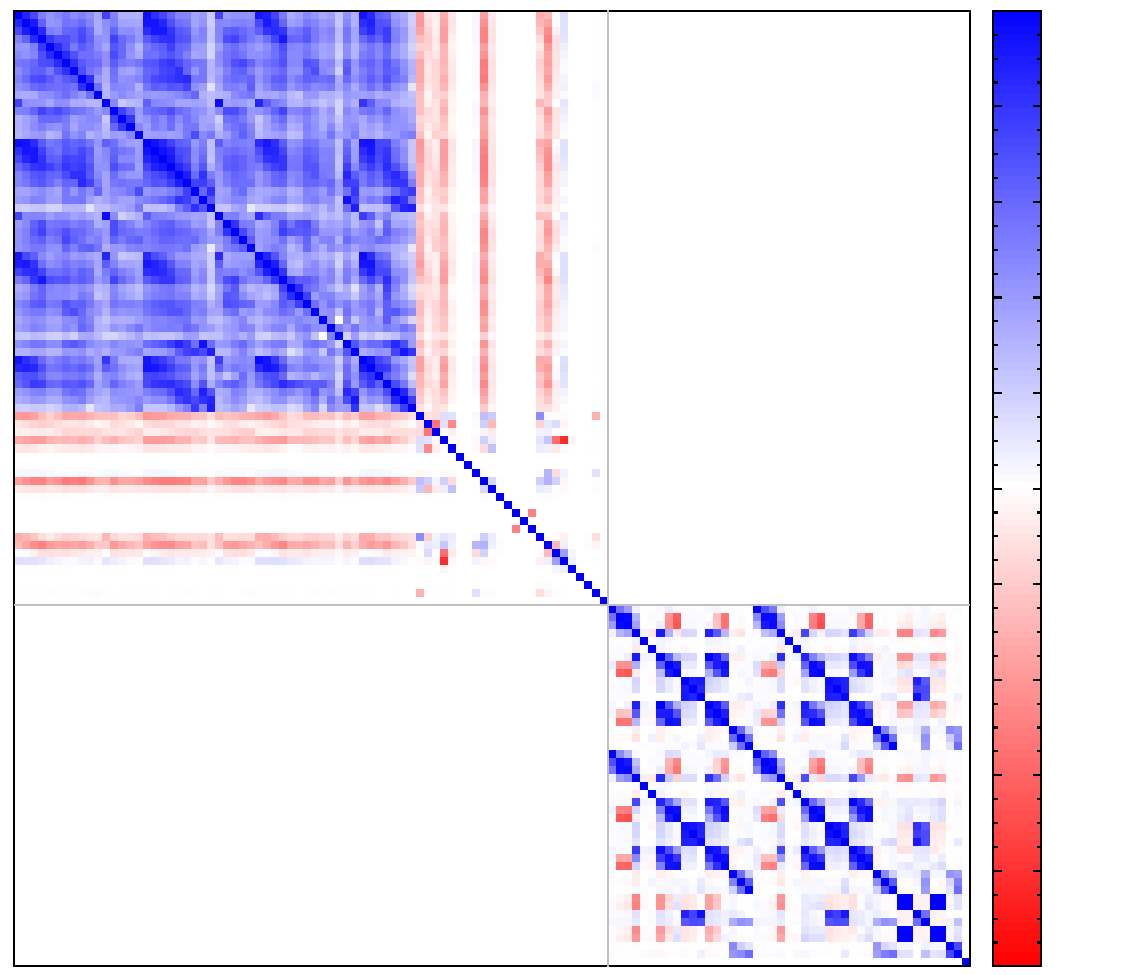
\includegraphics{pics/matrixplot}}%
    \gplfronttext
  \end{picture}%
\endgroup
}
	\caption[Correlation matrix of the beam systematic model]%
		{Correlation matrix of the beam systematic model.
		The two main blocks correspond to respectively the BANFF errors and the far detector %
		Final State interaction errors.}
	\label{fig:correlation}
\end{figure}

There are also 45 uncertainties for SK detector efficiencies and Final State Interactions (FSI),
which parameterise the uncertainties on the four final state event selections at the far detector. %
Among these, one uncorrelated systematic describes the energy scale uncertainty.
%The energy scale calibration of the far detector is a crucial step to scale systematic of SK is assumed to be valid for HK.
The reconstruction of the momenta in a neutrino event is mainly based on the charge collected by the PMTs, %
and therefore the resolution is limited by water quality and PMT gain.
A precise momentum determination of the incoming neutrino is a necessary requirement for oscillation analysis.
The calibration of the energy scale is therefore a crucial step and in SK it is performed %
using four well-known independent control samples~\cite{Abe:2017aap}.
%from 1\,GeV to 10\,GeV by high energy stopping muons; from 200\,MeV to 500\,MeV by low energy stopping muons;
%around 130\,MeV by neutral pions from neutrino interactions; %
%around 40\,MeV from decay electrons.
Since the energy loss $\dv*{E}{x}$ is approximately constant, %
the ratio between reconstructed momentum and track length of high energy stopping muon  %
is used to regulate the energy scale for energies in the range 1--10\,GeV.
The track is estimated from the entering position of the muon and the vertex of the detected Michel electron, %
both of which are assumed to be independent on the reconstruction method.
The momentum of low-energy stopping muons with energies from 200\,MeV to 500\,MeV are estimated by determining the %
Cherenkov angle using \refeqs{eq:cherenkov_threshold}{eq:cherenkov_angle}; %
only events with a clear Cherenkov ring and optimal reconstruction are selected, %
and the purity of the sample is improved by requiring the detection of the decay electron in the fiducial volume.
The single neutral pions produced in NC interactions of atmospheric neutrinos are reconstructed %
by looking at the invariant mass of the final state photons
\begin{equation}
	m_{\pi^0}^2 = 2\,p_{\gamma_1}\,p_{\gamma_2} (1-\cos\theta)\ ,
\end{equation}
with $\theta$ the opening angle between $\gamma_1$ and $\gamma_2$.
The error on the energy scale at around 130\,MeV comes from comparing the peak positions %
of the data and Monte Carlo distributions of $m_{\pi^0}$.
Finally, the distribution of decay electron events from stopping cosmic muons is used at energies around 40\,MeV.
This sample is used to test whether the detector response is uniform, since %
vertices and the direction of the electrons distribute homogeneously and isotropically in the fiducial volume.
The stability in time of the energy scale is instead validated by the high energy stopping muons.
The energy scale systematic of SK is assumed to be valid for HK.

The full list of systematics is reported in \refapp{cha:systematics}.
The correlation matrix between the beam systematics is shown as a 2D colour map on \reffig{fig:correlation}, %
from which the three main typologies of uncertainties -- flux, cross-section, and far detector -- %
are easily recognised.
The SK and FSI systematics are visibly uncorrelated with the BANFF ones.
%and the far detector energy scale error.



\subsection{Sensitivity with the nominal systematic model}
\label{sec:nominal}

Using the predictions from \refsec{sec:prediction} and fixing the \emph{true} oscillation parameter %
combination at the Asimov A point (see \reftab{tab:asimovA}), %
the $\chi^2$ profile is now calculated with the minimisation method in previous \refsec{sec:x2}.
A combined fit of the $\nu_e$ and $\nu_\mu$ samples allows to estimate the sensitivity of HK %
to the oscillation parameters.
The $\chi^2$ profiles against the variation of the oscillation parameters %
$\Delta m^2_{32}$, $\sin^2 2\theta_{13}$, $\sin^2 \theta_{23}$, and $\delta_\text{CP}$ %
are shown in \reffig{fig:nominal_profile}.
The contour plots of the $\chi^2$ with $\Delta m_{32}^2$ versus $\sin^2\theta_{23}$ and %
$\delta_\text{CP}$ and $\sin^2 2\theta_{13}$ are also shown.
The lines show also the effect of the Gaussian penalty term on the angle $\theta_{13}$ from reactor constraints.
Unsurprisingly, this term mostly affects the $\chi^2$ profile for $\sin^2 2\theta_{13}$ and slightly $\delta_\text{CP}$ %
as they are correlated.

\begin{figure}
	\centering
	\resizebox{0.49\linewidth}{!}{% GNUPLOT: LaTeX picture with Postscript
\begingroup
  \makeatletter
  \providecommand\color[2][]{%
    \GenericError{(gnuplot) \space\space\space\@spaces}{%
      Package color not loaded in conjunction with
      terminal option `colourtext'%
    }{See the gnuplot documentation for explanation.%
    }{Either use 'blacktext' in gnuplot or load the package
      color.sty in LaTeX.}%
    \renewcommand\color[2][]{}%
  }%
  \providecommand\includegraphics[2][]{%
    \GenericError{(gnuplot) \space\space\space\@spaces}{%
      Package graphicx or graphics not loaded%
    }{See the gnuplot documentation for explanation.%
    }{The gnuplot epslatex terminal needs graphicx.sty or graphics.sty.}%
    \renewcommand\includegraphics[2][]{}%
  }%
  \providecommand\rotatebox[2]{#2}%
  \@ifundefined{ifGPcolor}{%
    \newif\ifGPcolor
    \GPcolortrue
  }{}%
  \@ifundefined{ifGPblacktext}{%
    \newif\ifGPblacktext
    \GPblacktexttrue
  }{}%
  % define a \g@addto@macro without @ in the name:
  \let\gplgaddtomacro\g@addto@macro
  % define empty templates for all commands taking text:
  \gdef\gplbacktext{}%
  \gdef\gplfronttext{}%
  \makeatother
  \ifGPblacktext
    % no textcolor at all
    \def\colorrgb#1{}%
    \def\colorgray#1{}%
  \else
    % gray or color?
    \ifGPcolor
      \def\colorrgb#1{\color[rgb]{#1}}%
      \def\colorgray#1{\color[gray]{#1}}%
      \expandafter\def\csname LTw\endcsname{\color{white}}%
      \expandafter\def\csname LTb\endcsname{\color{black}}%
      \expandafter\def\csname LTa\endcsname{\color{black}}%
      \expandafter\def\csname LT0\endcsname{\color[rgb]{1,0,0}}%
      \expandafter\def\csname LT1\endcsname{\color[rgb]{0,1,0}}%
      \expandafter\def\csname LT2\endcsname{\color[rgb]{0,0,1}}%
      \expandafter\def\csname LT3\endcsname{\color[rgb]{1,0,1}}%
      \expandafter\def\csname LT4\endcsname{\color[rgb]{0,1,1}}%
      \expandafter\def\csname LT5\endcsname{\color[rgb]{1,1,0}}%
      \expandafter\def\csname LT6\endcsname{\color[rgb]{0,0,0}}%
      \expandafter\def\csname LT7\endcsname{\color[rgb]{1,0.3,0}}%
      \expandafter\def\csname LT8\endcsname{\color[rgb]{0.5,0.5,0.5}}%
    \else
      % gray
      \def\colorrgb#1{\color{black}}%
      \def\colorgray#1{\color[gray]{#1}}%
      \expandafter\def\csname LTw\endcsname{\color{white}}%
      \expandafter\def\csname LTb\endcsname{\color{black}}%
      \expandafter\def\csname LTa\endcsname{\color{black}}%
      \expandafter\def\csname LT0\endcsname{\color{black}}%
      \expandafter\def\csname LT1\endcsname{\color{black}}%
      \expandafter\def\csname LT2\endcsname{\color{black}}%
      \expandafter\def\csname LT3\endcsname{\color{black}}%
      \expandafter\def\csname LT4\endcsname{\color{black}}%
      \expandafter\def\csname LT5\endcsname{\color{black}}%
      \expandafter\def\csname LT6\endcsname{\color{black}}%
      \expandafter\def\csname LT7\endcsname{\color{black}}%
      \expandafter\def\csname LT8\endcsname{\color{black}}%
    \fi
  \fi
    \setlength{\unitlength}{0.0500bp}%
    \ifx\gptboxheight\undefined%
      \newlength{\gptboxheight}%
      \newlength{\gptboxwidth}%
      \newsavebox{\gptboxtext}%
    \fi%
    \setlength{\fboxrule}{0.5pt}%
    \setlength{\fboxsep}{1pt}%
\begin{picture}(7200.00,5760.00)%
    \gplgaddtomacro\gplbacktext{%
      \csname LTb\endcsname%%
      \put(618,864){\makebox(0,0)[r]{\strut{}-1}}%
      \csname LTb\endcsname%%
      \put(618,1267){\makebox(0,0)[r]{\strut{}1}}%
      \csname LTb\endcsname%%
      \put(618,1670){\makebox(0,0)[r]{\strut{}3}}%
      \csname LTb\endcsname%%
      \put(618,2074){\makebox(0,0)[r]{\strut{}5}}%
      \csname LTb\endcsname%%
      \put(618,2477){\makebox(0,0)[r]{\strut{}7}}%
      \csname LTb\endcsname%%
      \put(720,678){\makebox(0,0){\strut{}-1.00$\pi$}}%
      \csname LTb\endcsname%%
      \put(1524,678){\makebox(0,0){\strut{}-0.75$\pi$}}%
      \csname LTb\endcsname%%
      \put(2327,678){\makebox(0,0){\strut{}-0.50$\pi$}}%
      \csname LTb\endcsname%%
      \put(3131,678){\makebox(0,0){\strut{}-0.25$\pi$}}%
      \csname LTb\endcsname%%
      \put(3934,678){\makebox(0,0){\strut{}0.00$\pi$}}%
      \csname LTb\endcsname%%
      \put(4738,678){\makebox(0,0){\strut{}0.25$\pi$}}%
      \csname LTb\endcsname%%
      \put(5541,678){\makebox(0,0){\strut{}0.50$\pi$}}%
      \csname LTb\endcsname%%
      \put(6345,678){\makebox(0,0){\strut{}0.75$\pi$}}%
      \csname LTb\endcsname%%
      \put(7148,678){\makebox(0,0){\strut{}1.00$\pi$}}%
    }%
    \gplgaddtomacro\gplfronttext{%
      \csname LTb\endcsname%%
      \put(228,1872){\rotatebox{-270}{\makebox(0,0){\strut{}$\Delta \chi^2_0 - \Delta \chi^2$}}}%
      \csname LTb\endcsname%%
      \put(3934,399){\makebox(0,0){\strut{}$\delta_\text{CP}$}}%
    }%
    \gplgaddtomacro\gplbacktext{%
      \csname LTb\endcsname%%
      \put(618,2880){\makebox(0,0)[r]{\strut{}0}}%
      \csname LTb\endcsname%%
      \put(618,3499){\makebox(0,0)[r]{\strut{}40}}%
      \csname LTb\endcsname%%
      \put(618,4118){\makebox(0,0)[r]{\strut{}80}}%
      \csname LTb\endcsname%%
      \put(618,4737){\makebox(0,0)[r]{\strut{}120}}%
      \csname LTb\endcsname%%
      \put(618,5356){\makebox(0,0)[r]{\strut{}160}}%
      \csname LTb\endcsname%%
      \put(720,2694){\makebox(0,0){\strut{}}}%
      \csname LTb\endcsname%%
      \put(1524,2694){\makebox(0,0){\strut{}}}%
      \csname LTb\endcsname%%
      \put(2327,2694){\makebox(0,0){\strut{}}}%
      \csname LTb\endcsname%%
      \put(3131,2694){\makebox(0,0){\strut{}}}%
      \csname LTb\endcsname%%
      \put(3934,2694){\makebox(0,0){\strut{}}}%
      \csname LTb\endcsname%%
      \put(4738,2694){\makebox(0,0){\strut{}}}%
      \csname LTb\endcsname%%
      \put(5541,2694){\makebox(0,0){\strut{}}}%
      \csname LTb\endcsname%%
      \put(6345,2694){\makebox(0,0){\strut{}}}%
      \csname LTb\endcsname%%
      \put(7148,2694){\makebox(0,0){\strut{}}}%
    }%
    \gplgaddtomacro\gplfronttext{%
      \csname LTb\endcsname%%
      \put(126,4273){\rotatebox{-270}{\makebox(0,0){\strut{}$\Delta \chi^2$}}}%
      \csname LTb\endcsname%%
      \put(3934,2638){\makebox(0,0){\strut{}}}%
      \csname LTb\endcsname%%
      \put(3175,4877){\makebox(0,0){\strut{}}}%
      \csname LTb\endcsname%%
      \put(3572,4877){\makebox(0,0)[r]{\strut{}w/ penalty}}%
      \csname LTb\endcsname%%
      \put(3572,4691){\makebox(0,0)[r]{\strut{}w/o penalty}}%
    }%
    \gplbacktext
    \put(0,0){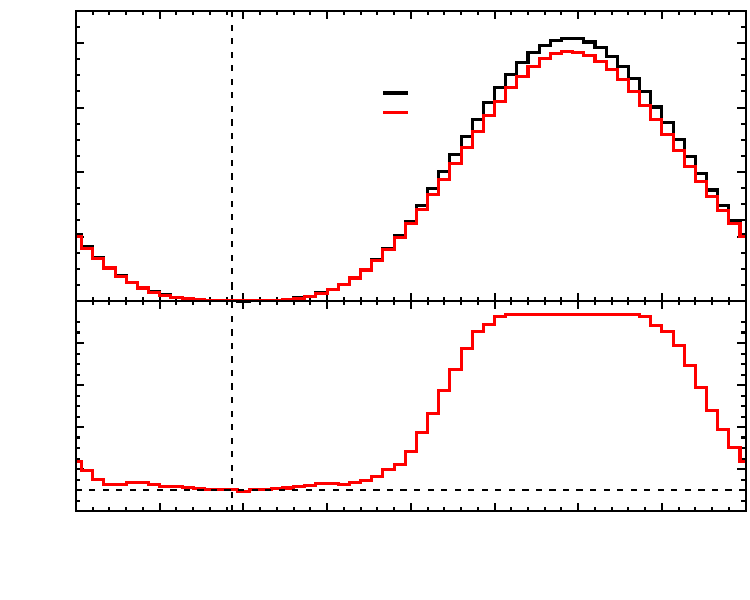
\includegraphics{pics/just0_chi2_dCP}}%
    \gplfronttext
  \end{picture}%
\endgroup
}
	\resizebox{0.49\linewidth}{!}{% GNUPLOT: LaTeX picture with Postscript
\begingroup
  \makeatletter
  \providecommand\color[2][]{%
    \GenericError{(gnuplot) \space\space\space\@spaces}{%
      Package color not loaded in conjunction with
      terminal option `colourtext'%
    }{See the gnuplot documentation for explanation.%
    }{Either use 'blacktext' in gnuplot or load the package
      color.sty in LaTeX.}%
    \renewcommand\color[2][]{}%
  }%
  \providecommand\includegraphics[2][]{%
    \GenericError{(gnuplot) \space\space\space\@spaces}{%
      Package graphicx or graphics not loaded%
    }{See the gnuplot documentation for explanation.%
    }{The gnuplot epslatex terminal needs graphicx.sty or graphics.sty.}%
    \renewcommand\includegraphics[2][]{}%
  }%
  \providecommand\rotatebox[2]{#2}%
  \@ifundefined{ifGPcolor}{%
    \newif\ifGPcolor
    \GPcolortrue
  }{}%
  \@ifundefined{ifGPblacktext}{%
    \newif\ifGPblacktext
    \GPblacktexttrue
  }{}%
  % define a \g@addto@macro without @ in the name:
  \let\gplgaddtomacro\g@addto@macro
  % define empty templates for all commands taking text:
  \gdef\gplbacktext{}%
  \gdef\gplfronttext{}%
  \makeatother
  \ifGPblacktext
    % no textcolor at all
    \def\colorrgb#1{}%
    \def\colorgray#1{}%
  \else
    % gray or color?
    \ifGPcolor
      \def\colorrgb#1{\color[rgb]{#1}}%
      \def\colorgray#1{\color[gray]{#1}}%
      \expandafter\def\csname LTw\endcsname{\color{white}}%
      \expandafter\def\csname LTb\endcsname{\color{black}}%
      \expandafter\def\csname LTa\endcsname{\color{black}}%
      \expandafter\def\csname LT0\endcsname{\color[rgb]{1,0,0}}%
      \expandafter\def\csname LT1\endcsname{\color[rgb]{0,1,0}}%
      \expandafter\def\csname LT2\endcsname{\color[rgb]{0,0,1}}%
      \expandafter\def\csname LT3\endcsname{\color[rgb]{1,0,1}}%
      \expandafter\def\csname LT4\endcsname{\color[rgb]{0,1,1}}%
      \expandafter\def\csname LT5\endcsname{\color[rgb]{1,1,0}}%
      \expandafter\def\csname LT6\endcsname{\color[rgb]{0,0,0}}%
      \expandafter\def\csname LT7\endcsname{\color[rgb]{1,0.3,0}}%
      \expandafter\def\csname LT8\endcsname{\color[rgb]{0.5,0.5,0.5}}%
    \else
      % gray
      \def\colorrgb#1{\color{black}}%
      \def\colorgray#1{\color[gray]{#1}}%
      \expandafter\def\csname LTw\endcsname{\color{white}}%
      \expandafter\def\csname LTb\endcsname{\color{black}}%
      \expandafter\def\csname LTa\endcsname{\color{black}}%
      \expandafter\def\csname LT0\endcsname{\color{black}}%
      \expandafter\def\csname LT1\endcsname{\color{black}}%
      \expandafter\def\csname LT2\endcsname{\color{black}}%
      \expandafter\def\csname LT3\endcsname{\color{black}}%
      \expandafter\def\csname LT4\endcsname{\color{black}}%
      \expandafter\def\csname LT5\endcsname{\color{black}}%
      \expandafter\def\csname LT6\endcsname{\color{black}}%
      \expandafter\def\csname LT7\endcsname{\color{black}}%
      \expandafter\def\csname LT8\endcsname{\color{black}}%
    \fi
  \fi
    \setlength{\unitlength}{0.0500bp}%
    \ifx\gptboxheight\undefined%
      \newlength{\gptboxheight}%
      \newlength{\gptboxwidth}%
      \newsavebox{\gptboxtext}%
    \fi%
    \setlength{\fboxrule}{0.5pt}%
    \setlength{\fboxsep}{1pt}%
\begin{picture}(7200.00,5760.00)%
    \gplgaddtomacro\gplbacktext{%
      \csname LTb\endcsname%%
      \put(618,864){\makebox(0,0)[r]{\strut{}-1}}%
      \csname LTb\endcsname%%
      \put(618,1231){\makebox(0,0)[r]{\strut{}1}}%
      \csname LTb\endcsname%%
      \put(618,1597){\makebox(0,0)[r]{\strut{}3}}%
      \csname LTb\endcsname%%
      \put(618,1964){\makebox(0,0)[r]{\strut{}5}}%
      \csname LTb\endcsname%%
      \put(618,2330){\makebox(0,0)[r]{\strut{}7}}%
      \csname LTb\endcsname%%
      \put(618,2697){\makebox(0,0)[r]{\strut{}9}}%
      \csname LTb\endcsname%%
      \put(720,678){\makebox(0,0){\strut{}0.07}}%
      \csname LTb\endcsname%%
      \put(1791,678){\makebox(0,0){\strut{}0.075}}%
      \csname LTb\endcsname%%
      \put(2863,678){\makebox(0,0){\strut{}0.08}}%
      \csname LTb\endcsname%%
      \put(3934,678){\makebox(0,0){\strut{}0.085}}%
      \csname LTb\endcsname%%
      \put(5005,678){\makebox(0,0){\strut{}0.09}}%
      \csname LTb\endcsname%%
      \put(6077,678){\makebox(0,0){\strut{}0.095}}%
      \csname LTb\endcsname%%
      \put(7148,678){\makebox(0,0){\strut{}0.1}}%
    }%
    \gplgaddtomacro\gplfronttext{%
      \csname LTb\endcsname%%
      \put(228,1872){\rotatebox{-270}{\makebox(0,0){\strut{}$\Delta \chi^2_0 - \Delta \chi^2$}}}%
      \csname LTb\endcsname%%
      \put(3934,399){\makebox(0,0){\strut{}$\sin^2 2 \theta_{13}$}}%
    }%
    \gplgaddtomacro\gplbacktext{%
      \csname LTb\endcsname%%
      \put(618,2880){\makebox(0,0)[r]{\strut{}0}}%
      \csname LTb\endcsname%%
      \put(618,3437){\makebox(0,0)[r]{\strut{}5}}%
      \csname LTb\endcsname%%
      \put(618,3994){\makebox(0,0)[r]{\strut{}10}}%
      \csname LTb\endcsname%%
      \put(618,4552){\makebox(0,0)[r]{\strut{}15}}%
      \csname LTb\endcsname%%
      \put(618,5109){\makebox(0,0)[r]{\strut{}20}}%
      \csname LTb\endcsname%%
      \put(618,5666){\makebox(0,0)[r]{\strut{}25}}%
      \csname LTb\endcsname%%
      \put(720,2694){\makebox(0,0){\strut{}}}%
      \csname LTb\endcsname%%
      \put(1791,2694){\makebox(0,0){\strut{}}}%
      \csname LTb\endcsname%%
      \put(2863,2694){\makebox(0,0){\strut{}}}%
      \csname LTb\endcsname%%
      \put(3934,2694){\makebox(0,0){\strut{}}}%
      \csname LTb\endcsname%%
      \put(5005,2694){\makebox(0,0){\strut{}}}%
      \csname LTb\endcsname%%
      \put(6077,2694){\makebox(0,0){\strut{}}}%
      \csname LTb\endcsname%%
      \put(7148,2694){\makebox(0,0){\strut{}}}%
    }%
    \gplgaddtomacro\gplfronttext{%
      \csname LTb\endcsname%%
      \put(228,4273){\rotatebox{-270}{\makebox(0,0){\strut{}$\Delta \chi^2$}}}%
      \csname LTb\endcsname%%
      \put(3934,2638){\makebox(0,0){\strut{}}}%
      \csname LTb\endcsname%%
      \put(4903,4877){\makebox(0,0){\strut{}}}%
      \csname LTb\endcsname%%
      \put(5300,4877){\makebox(0,0)[r]{\strut{}w/ penalty}}%
      \csname LTb\endcsname%%
      \put(5300,4691){\makebox(0,0)[r]{\strut{}w/o penalty}}%
    }%
    \gplbacktext
    \put(0,0){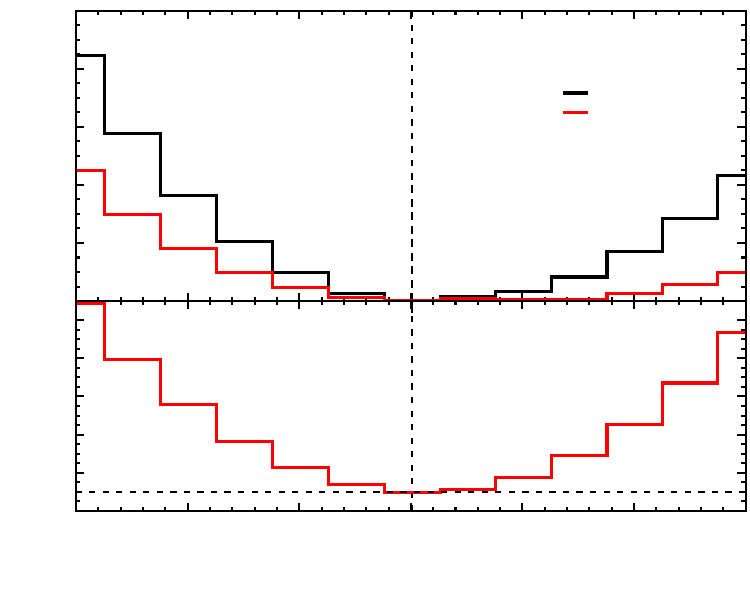
\includegraphics{pics/just0_chi2_S13}}%
    \gplfronttext
  \end{picture}%
\endgroup
}
	\resizebox{0.49\linewidth}{!}{% GNUPLOT: LaTeX picture with Postscript
\begingroup
  \makeatletter
  \providecommand\color[2][]{%
    \GenericError{(gnuplot) \space\space\space\@spaces}{%
      Package color not loaded in conjunction with
      terminal option `colourtext'%
    }{See the gnuplot documentation for explanation.%
    }{Either use 'blacktext' in gnuplot or load the package
      color.sty in LaTeX.}%
    \renewcommand\color[2][]{}%
  }%
  \providecommand\includegraphics[2][]{%
    \GenericError{(gnuplot) \space\space\space\@spaces}{%
      Package graphicx or graphics not loaded%
    }{See the gnuplot documentation for explanation.%
    }{The gnuplot epslatex terminal needs graphicx.sty or graphics.sty.}%
    \renewcommand\includegraphics[2][]{}%
  }%
  \providecommand\rotatebox[2]{#2}%
  \@ifundefined{ifGPcolor}{%
    \newif\ifGPcolor
    \GPcolortrue
  }{}%
  \@ifundefined{ifGPblacktext}{%
    \newif\ifGPblacktext
    \GPblacktexttrue
  }{}%
  % define a \g@addto@macro without @ in the name:
  \let\gplgaddtomacro\g@addto@macro
  % define empty templates for all commands taking text:
  \gdef\gplbacktext{}%
  \gdef\gplfronttext{}%
  \makeatother
  \ifGPblacktext
    % no textcolor at all
    \def\colorrgb#1{}%
    \def\colorgray#1{}%
  \else
    % gray or color?
    \ifGPcolor
      \def\colorrgb#1{\color[rgb]{#1}}%
      \def\colorgray#1{\color[gray]{#1}}%
      \expandafter\def\csname LTw\endcsname{\color{white}}%
      \expandafter\def\csname LTb\endcsname{\color{black}}%
      \expandafter\def\csname LTa\endcsname{\color{black}}%
      \expandafter\def\csname LT0\endcsname{\color[rgb]{1,0,0}}%
      \expandafter\def\csname LT1\endcsname{\color[rgb]{0,1,0}}%
      \expandafter\def\csname LT2\endcsname{\color[rgb]{0,0,1}}%
      \expandafter\def\csname LT3\endcsname{\color[rgb]{1,0,1}}%
      \expandafter\def\csname LT4\endcsname{\color[rgb]{0,1,1}}%
      \expandafter\def\csname LT5\endcsname{\color[rgb]{1,1,0}}%
      \expandafter\def\csname LT6\endcsname{\color[rgb]{0,0,0}}%
      \expandafter\def\csname LT7\endcsname{\color[rgb]{1,0.3,0}}%
      \expandafter\def\csname LT8\endcsname{\color[rgb]{0.5,0.5,0.5}}%
    \else
      % gray
      \def\colorrgb#1{\color{black}}%
      \def\colorgray#1{\color[gray]{#1}}%
      \expandafter\def\csname LTw\endcsname{\color{white}}%
      \expandafter\def\csname LTb\endcsname{\color{black}}%
      \expandafter\def\csname LTa\endcsname{\color{black}}%
      \expandafter\def\csname LT0\endcsname{\color{black}}%
      \expandafter\def\csname LT1\endcsname{\color{black}}%
      \expandafter\def\csname LT2\endcsname{\color{black}}%
      \expandafter\def\csname LT3\endcsname{\color{black}}%
      \expandafter\def\csname LT4\endcsname{\color{black}}%
      \expandafter\def\csname LT5\endcsname{\color{black}}%
      \expandafter\def\csname LT6\endcsname{\color{black}}%
      \expandafter\def\csname LT7\endcsname{\color{black}}%
      \expandafter\def\csname LT8\endcsname{\color{black}}%
    \fi
  \fi
    \setlength{\unitlength}{0.0500bp}%
    \ifx\gptboxheight\undefined%
      \newlength{\gptboxheight}%
      \newlength{\gptboxwidth}%
      \newsavebox{\gptboxtext}%
    \fi%
    \setlength{\fboxrule}{0.5pt}%
    \setlength{\fboxsep}{1pt}%
\begin{picture}(7200.00,5760.00)%
    \gplgaddtomacro\gplbacktext{%
      \csname LTb\endcsname%%
      \put(618,864){\makebox(0,0)[r]{\strut{}-0.1}}%
      \csname LTb\endcsname%%
      \put(618,1368){\makebox(0,0)[r]{\strut{}0}}%
      \csname LTb\endcsname%%
      \put(618,1872){\makebox(0,0)[r]{\strut{}0.1}}%
      \csname LTb\endcsname%%
      \put(618,2376){\makebox(0,0)[r]{\strut{}0.2}}%
      \csname LTb\endcsname%%
      \put(720,678){\makebox(0,0){\strut{}2.464}}%
      \csname LTb\endcsname%%
      \put(1791,678){\makebox(0,0){\strut{}2.479}}%
      \csname LTb\endcsname%%
      \put(2863,678){\makebox(0,0){\strut{}2.494}}%
      \csname LTb\endcsname%%
      \put(3934,678){\makebox(0,0){\strut{}2.509}}%
      \csname LTb\endcsname%%
      \put(5005,678){\makebox(0,0){\strut{}2.524}}%
      \csname LTb\endcsname%%
      \put(6077,678){\makebox(0,0){\strut{}2.539}}%
      \csname LTb\endcsname%%
      \put(7148,678){\makebox(0,0){\strut{}2.554}}%
    }%
    \gplgaddtomacro\gplfronttext{%
      \csname LTb\endcsname%%
      \put(24,1872){\rotatebox{-270}{\makebox(0,0){\strut{}$\Delta \chi^2_\text{w/} - \Delta \chi^2_\text{w/o}$}}}%
      \csname LTb\endcsname%%
      \put(3934,399){\makebox(0,0){\strut{}$\Delta m_{32}^2 / 10^{-3}$}}%
    }%
    \gplgaddtomacro\gplbacktext{%
      \csname LTb\endcsname%%
      \put(618,2880){\makebox(0,0)[r]{\strut{}0}}%
      \csname LTb\endcsname%%
      \put(618,4273){\makebox(0,0)[r]{\strut{}5}}%
      \csname LTb\endcsname%%
      \put(618,5666){\makebox(0,0)[r]{\strut{}10}}%
      \csname LTb\endcsname%%
      \put(720,2694){\makebox(0,0){\strut{}}}%
      \csname LTb\endcsname%%
      \put(1791,2694){\makebox(0,0){\strut{}}}%
      \csname LTb\endcsname%%
      \put(2863,2694){\makebox(0,0){\strut{}}}%
      \csname LTb\endcsname%%
      \put(3934,2694){\makebox(0,0){\strut{}}}%
      \csname LTb\endcsname%%
      \put(5005,2694){\makebox(0,0){\strut{}}}%
      \csname LTb\endcsname%%
      \put(6077,2694){\makebox(0,0){\strut{}}}%
      \csname LTb\endcsname%%
      \put(7148,2694){\makebox(0,0){\strut{}}}%
    }%
    \gplgaddtomacro\gplfronttext{%
      \csname LTb\endcsname%%
      \put(228,4273){\rotatebox{-270}{\makebox(0,0){\strut{}$\Delta \chi^2$}}}%
      \csname LTb\endcsname%%
      \put(3934,2638){\makebox(0,0){\strut{}}}%
      \csname LTb\endcsname%%
      \put(4890,4877){\makebox(0,0){\strut{}}}%
      \csname LTb\endcsname%%
      \put(5287,4877){\makebox(0,0)[r]{\strut{}w/ penalty}}%
      \csname LTb\endcsname%%
      \put(5287,4691){\makebox(0,0)[r]{\strut{}w/o penalty}}%
    }%
    \gplbacktext
    \put(0,0){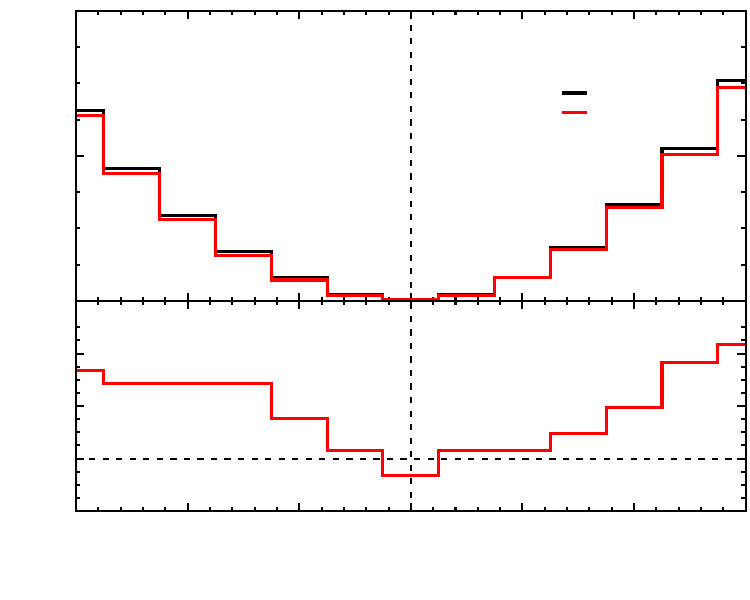
\includegraphics{pics/just0_chi2_M23}}%
    \gplfronttext
  \end{picture}%
\endgroup
}
	\resizebox{0.49\linewidth}{!}{% GNUPLOT: LaTeX picture with Postscript
\begingroup
  \makeatletter
  \providecommand\color[2][]{%
    \GenericError{(gnuplot) \space\space\space\@spaces}{%
      Package color not loaded in conjunction with
      terminal option `colourtext'%
    }{See the gnuplot documentation for explanation.%
    }{Either use 'blacktext' in gnuplot or load the package
      color.sty in LaTeX.}%
    \renewcommand\color[2][]{}%
  }%
  \providecommand\includegraphics[2][]{%
    \GenericError{(gnuplot) \space\space\space\@spaces}{%
      Package graphicx or graphics not loaded%
    }{See the gnuplot documentation for explanation.%
    }{The gnuplot epslatex terminal needs graphicx.sty or graphics.sty.}%
    \renewcommand\includegraphics[2][]{}%
  }%
  \providecommand\rotatebox[2]{#2}%
  \@ifundefined{ifGPcolor}{%
    \newif\ifGPcolor
    \GPcolortrue
  }{}%
  \@ifundefined{ifGPblacktext}{%
    \newif\ifGPblacktext
    \GPblacktexttrue
  }{}%
  % define a \g@addto@macro without @ in the name:
  \let\gplgaddtomacro\g@addto@macro
  % define empty templates for all commands taking text:
  \gdef\gplbacktext{}%
  \gdef\gplfronttext{}%
  \makeatother
  \ifGPblacktext
    % no textcolor at all
    \def\colorrgb#1{}%
    \def\colorgray#1{}%
  \else
    % gray or color?
    \ifGPcolor
      \def\colorrgb#1{\color[rgb]{#1}}%
      \def\colorgray#1{\color[gray]{#1}}%
      \expandafter\def\csname LTw\endcsname{\color{white}}%
      \expandafter\def\csname LTb\endcsname{\color{black}}%
      \expandafter\def\csname LTa\endcsname{\color{black}}%
      \expandafter\def\csname LT0\endcsname{\color[rgb]{1,0,0}}%
      \expandafter\def\csname LT1\endcsname{\color[rgb]{0,1,0}}%
      \expandafter\def\csname LT2\endcsname{\color[rgb]{0,0,1}}%
      \expandafter\def\csname LT3\endcsname{\color[rgb]{1,0,1}}%
      \expandafter\def\csname LT4\endcsname{\color[rgb]{0,1,1}}%
      \expandafter\def\csname LT5\endcsname{\color[rgb]{1,1,0}}%
      \expandafter\def\csname LT6\endcsname{\color[rgb]{0,0,0}}%
      \expandafter\def\csname LT7\endcsname{\color[rgb]{1,0.3,0}}%
      \expandafter\def\csname LT8\endcsname{\color[rgb]{0.5,0.5,0.5}}%
    \else
      % gray
      \def\colorrgb#1{\color{black}}%
      \def\colorgray#1{\color[gray]{#1}}%
      \expandafter\def\csname LTw\endcsname{\color{white}}%
      \expandafter\def\csname LTb\endcsname{\color{black}}%
      \expandafter\def\csname LTa\endcsname{\color{black}}%
      \expandafter\def\csname LT0\endcsname{\color{black}}%
      \expandafter\def\csname LT1\endcsname{\color{black}}%
      \expandafter\def\csname LT2\endcsname{\color{black}}%
      \expandafter\def\csname LT3\endcsname{\color{black}}%
      \expandafter\def\csname LT4\endcsname{\color{black}}%
      \expandafter\def\csname LT5\endcsname{\color{black}}%
      \expandafter\def\csname LT6\endcsname{\color{black}}%
      \expandafter\def\csname LT7\endcsname{\color{black}}%
      \expandafter\def\csname LT8\endcsname{\color{black}}%
    \fi
  \fi
    \setlength{\unitlength}{0.0500bp}%
    \ifx\gptboxheight\undefined%
      \newlength{\gptboxheight}%
      \newlength{\gptboxwidth}%
      \newsavebox{\gptboxtext}%
    \fi%
    \setlength{\fboxrule}{0.5pt}%
    \setlength{\fboxsep}{1pt}%
\begin{picture}(7200.00,5760.00)%
    \gplgaddtomacro\gplbacktext{%
      \csname LTb\endcsname%%
      \put(618,864){\makebox(0,0)[r]{\strut{}-1}}%
      \csname LTb\endcsname%%
      \put(618,1440){\makebox(0,0)[r]{\strut{}1}}%
      \csname LTb\endcsname%%
      \put(618,2016){\makebox(0,0)[r]{\strut{}3}}%
      \csname LTb\endcsname%%
      \put(618,2592){\makebox(0,0)[r]{\strut{}5}}%
      \csname LTb\endcsname%%
      \put(720,678){\makebox(0,0){\strut{}0.426}}%
      \csname LTb\endcsname%%
      \put(1791,678){\makebox(0,0){\strut{}0.4515}}%
      \csname LTb\endcsname%%
      \put(2863,678){\makebox(0,0){\strut{}0.477}}%
      \csname LTb\endcsname%%
      \put(3934,678){\makebox(0,0){\strut{}0.5025}}%
      \csname LTb\endcsname%%
      \put(5005,678){\makebox(0,0){\strut{}0.528}}%
      \csname LTb\endcsname%%
      \put(6077,678){\makebox(0,0){\strut{}0.5535}}%
      \csname LTb\endcsname%%
      \put(7148,678){\makebox(0,0){\strut{}0.579}}%
    }%
    \gplgaddtomacro\gplfronttext{%
      \csname LTb\endcsname%%
      \put(228,1872){\rotatebox{-270}{\makebox(0,0){\strut{}$\Delta \chi^2_0 - \Delta \chi^2$}}}%
      \csname LTb\endcsname%%
      \put(3934,399){\makebox(0,0){\strut{}$\sin^2 \theta_{23}$}}%
    }%
    \gplgaddtomacro\gplbacktext{%
      \csname LTb\endcsname%%
      \put(618,2880){\makebox(0,0)[r]{\strut{}0}}%
      \csname LTb\endcsname%%
      \put(618,3344){\makebox(0,0)[r]{\strut{}20}}%
      \csname LTb\endcsname%%
      \put(618,3809){\makebox(0,0)[r]{\strut{}40}}%
      \csname LTb\endcsname%%
      \put(618,4273){\makebox(0,0)[r]{\strut{}60}}%
      \csname LTb\endcsname%%
      \put(618,4737){\makebox(0,0)[r]{\strut{}80}}%
      \csname LTb\endcsname%%
      \put(618,5202){\makebox(0,0)[r]{\strut{}100}}%
      \csname LTb\endcsname%%
      \put(618,5666){\makebox(0,0)[r]{\strut{}120}}%
      \csname LTb\endcsname%%
      \put(720,2694){\makebox(0,0){\strut{}}}%
      \csname LTb\endcsname%%
      \put(1791,2694){\makebox(0,0){\strut{}}}%
      \csname LTb\endcsname%%
      \put(2863,2694){\makebox(0,0){\strut{}}}%
      \csname LTb\endcsname%%
      \put(3934,2694){\makebox(0,0){\strut{}}}%
      \csname LTb\endcsname%%
      \put(5005,2694){\makebox(0,0){\strut{}}}%
      \csname LTb\endcsname%%
      \put(6077,2694){\makebox(0,0){\strut{}}}%
      \csname LTb\endcsname%%
      \put(7148,2694){\makebox(0,0){\strut{}}}%
    }%
    \gplgaddtomacro\gplfronttext{%
      \csname LTb\endcsname%%
      \put(126,4273){\rotatebox{-270}{\makebox(0,0){\strut{}$\Delta \chi^2$}}}%
      \csname LTb\endcsname%%
      \put(3934,2638){\makebox(0,0){\strut{}}}%
      \csname LTb\endcsname%%
      \put(5961,4877){\makebox(0,0){\strut{}}}%
      \csname LTb\endcsname%%
      \put(6358,4877){\makebox(0,0)[r]{\strut{}w/ penalty}}%
      \csname LTb\endcsname%%
      \put(6358,4691){\makebox(0,0)[r]{\strut{}w/o penalty}}%
    }%
    \gplbacktext
    \put(0,0){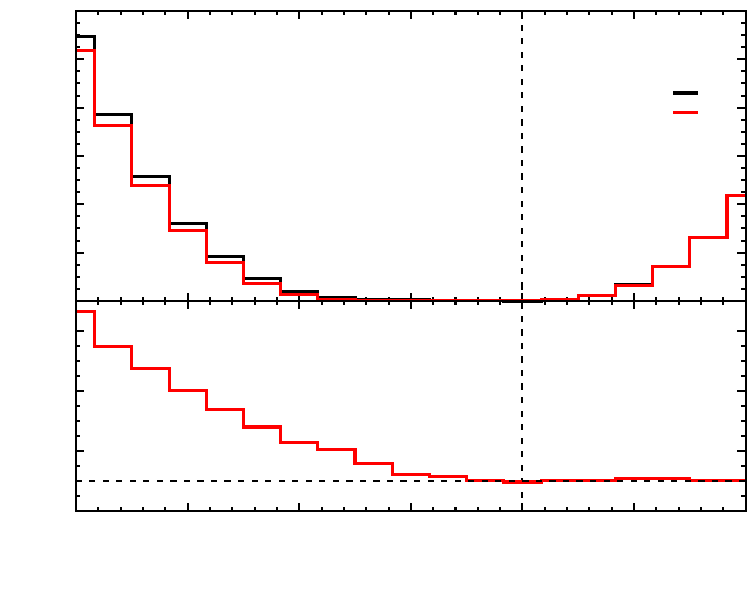
\includegraphics{pics/just0_chi2_S23}}%
    \gplfronttext
  \end{picture}%
\endgroup
}
	\resizebox{0.49\linewidth}{!}{% GNUPLOT: LaTeX picture with Postscript
\begingroup
  \makeatletter
  \providecommand\color[2][]{%
    \GenericError{(gnuplot) \space\space\space\@spaces}{%
      Package color not loaded in conjunction with
      terminal option `colourtext'%
    }{See the gnuplot documentation for explanation.%
    }{Either use 'blacktext' in gnuplot or load the package
      color.sty in LaTeX.}%
    \renewcommand\color[2][]{}%
  }%
  \providecommand\includegraphics[2][]{%
    \GenericError{(gnuplot) \space\space\space\@spaces}{%
      Package graphicx or graphics not loaded%
    }{See the gnuplot documentation for explanation.%
    }{The gnuplot epslatex terminal needs graphicx.sty or graphics.sty.}%
    \renewcommand\includegraphics[2][]{}%
  }%
  \providecommand\rotatebox[2]{#2}%
  \@ifundefined{ifGPcolor}{%
    \newif\ifGPcolor
    \GPcolortrue
  }{}%
  \@ifundefined{ifGPblacktext}{%
    \newif\ifGPblacktext
    \GPblacktexttrue
  }{}%
  % define a \g@addto@macro without @ in the name:
  \let\gplgaddtomacro\g@addto@macro
  % define empty templates for all commands taking text:
  \gdef\gplbacktext{}%
  \gdef\gplfronttext{}%
  \makeatother
  \ifGPblacktext
    % no textcolor at all
    \def\colorrgb#1{}%
    \def\colorgray#1{}%
  \else
    % gray or color?
    \ifGPcolor
      \def\colorrgb#1{\color[rgb]{#1}}%
      \def\colorgray#1{\color[gray]{#1}}%
      \expandafter\def\csname LTw\endcsname{\color{white}}%
      \expandafter\def\csname LTb\endcsname{\color{black}}%
      \expandafter\def\csname LTa\endcsname{\color{black}}%
      \expandafter\def\csname LT0\endcsname{\color[rgb]{1,0,0}}%
      \expandafter\def\csname LT1\endcsname{\color[rgb]{0,1,0}}%
      \expandafter\def\csname LT2\endcsname{\color[rgb]{0,0,1}}%
      \expandafter\def\csname LT3\endcsname{\color[rgb]{1,0,1}}%
      \expandafter\def\csname LT4\endcsname{\color[rgb]{0,1,1}}%
      \expandafter\def\csname LT5\endcsname{\color[rgb]{1,1,0}}%
      \expandafter\def\csname LT6\endcsname{\color[rgb]{0,0,0}}%
      \expandafter\def\csname LT7\endcsname{\color[rgb]{1,0.3,0}}%
      \expandafter\def\csname LT8\endcsname{\color[rgb]{0.5,0.5,0.5}}%
    \else
      % gray
      \def\colorrgb#1{\color{black}}%
      \def\colorgray#1{\color[gray]{#1}}%
      \expandafter\def\csname LTw\endcsname{\color{white}}%
      \expandafter\def\csname LTb\endcsname{\color{black}}%
      \expandafter\def\csname LTa\endcsname{\color{black}}%
      \expandafter\def\csname LT0\endcsname{\color{black}}%
      \expandafter\def\csname LT1\endcsname{\color{black}}%
      \expandafter\def\csname LT2\endcsname{\color{black}}%
      \expandafter\def\csname LT3\endcsname{\color{black}}%
      \expandafter\def\csname LT4\endcsname{\color{black}}%
      \expandafter\def\csname LT5\endcsname{\color{black}}%
      \expandafter\def\csname LT6\endcsname{\color{black}}%
      \expandafter\def\csname LT7\endcsname{\color{black}}%
      \expandafter\def\csname LT8\endcsname{\color{black}}%
    \fi
  \fi
    \setlength{\unitlength}{0.0500bp}%
    \ifx\gptboxheight\undefined%
      \newlength{\gptboxheight}%
      \newlength{\gptboxwidth}%
      \newsavebox{\gptboxtext}%
    \fi%
    \setlength{\fboxrule}{0.5pt}%
    \setlength{\fboxsep}{1pt}%
\begin{picture}(7200.00,5760.00)%
    \gplgaddtomacro\gplbacktext{%
      \csname LTb\endcsname%%
      \put(747,927){\makebox(0,0)[r]{\strut{}2.47}}%
      \csname LTb\endcsname%%
      \put(747,1480){\makebox(0,0)[r]{\strut{}2.48}}%
      \csname LTb\endcsname%%
      \put(747,2033){\makebox(0,0)[r]{\strut{}2.49}}%
      \csname LTb\endcsname%%
      \put(747,2586){\makebox(0,0)[r]{\strut{}2.5}}%
      \csname LTb\endcsname%%
      \put(747,3139){\makebox(0,0)[r]{\strut{}2.51}}%
      \csname LTb\endcsname%%
      \put(747,3692){\makebox(0,0)[r]{\strut{}2.52}}%
      \csname LTb\endcsname%%
      \put(747,4246){\makebox(0,0)[r]{\strut{}2.53}}%
      \csname LTb\endcsname%%
      \put(747,4799){\makebox(0,0)[r]{\strut{}2.54}}%
      \csname LTb\endcsname%%
      \put(747,5352){\makebox(0,0)[r]{\strut{}2.55}}%
      \csname LTb\endcsname%%
      \put(1402,409){\makebox(0,0){\strut{}0.44}}%
      \csname LTb\endcsname%%
      \put(2192,409){\makebox(0,0){\strut{}0.46}}%
      \csname LTb\endcsname%%
      \put(2982,409){\makebox(0,0){\strut{}0.48}}%
      \csname LTb\endcsname%%
      \put(3772,409){\makebox(0,0){\strut{}0.5}}%
      \csname LTb\endcsname%%
      \put(4562,409){\makebox(0,0){\strut{}0.52}}%
      \csname LTb\endcsname%%
      \put(5352,409){\makebox(0,0){\strut{}0.54}}%
      \csname LTb\endcsname%%
      \put(6142,409){\makebox(0,0){\strut{}0.56}}%
      \csname LTb\endcsname%%
      \put(4915,3121){\makebox(0,0)[l]{\strut{}}}%
    }%
    \gplgaddtomacro\gplfronttext{%
      \csname LTb\endcsname%%
      \put(153,3084){\rotatebox{-270}{\makebox(0,0){\strut{}$\Delta m_{32}^2 / 10^{-3}$}}}%
      \csname LTb\endcsname%%
      \put(3871,130){\makebox(0,0){\strut{}$\sin^2 \theta_{23}$}}%
      \csname LTb\endcsname%%
      \put(6360,5406){\makebox(0,0)[r]{\strut{}w/ penalty}}%
      \csname LTb\endcsname%%
      \put(6360,5220){\makebox(0,0)[r]{\strut{}w/o penalty}}%
    }%
    \gplbacktext
    \put(0,0){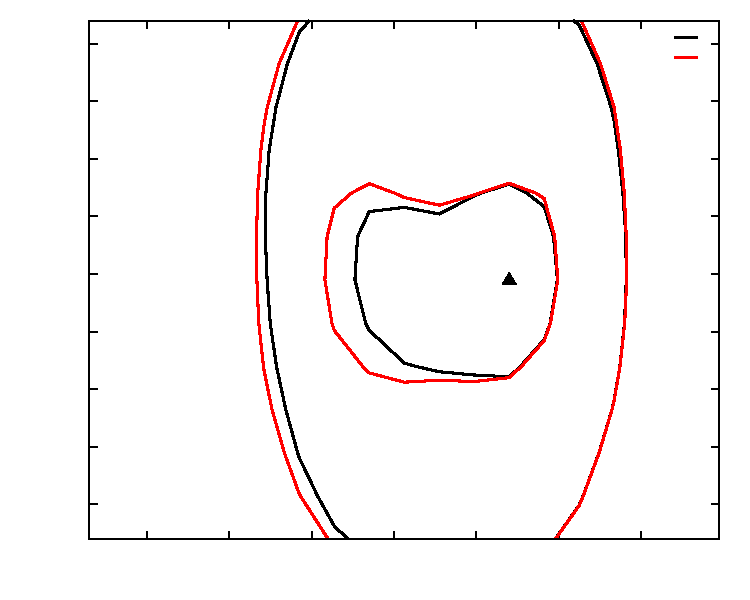
\includegraphics{pics/just0_cont_S23_M23}}%
    \gplfronttext
  \end{picture}%
\endgroup
}	%%%%%%%%%%%this is important
	\resizebox{0.49\linewidth}{!}{% GNUPLOT: LaTeX picture with Postscript
\begingroup
  \makeatletter
  \providecommand\color[2][]{%
    \GenericError{(gnuplot) \space\space\space\@spaces}{%
      Package color not loaded in conjunction with
      terminal option `colourtext'%
    }{See the gnuplot documentation for explanation.%
    }{Either use 'blacktext' in gnuplot or load the package
      color.sty in LaTeX.}%
    \renewcommand\color[2][]{}%
  }%
  \providecommand\includegraphics[2][]{%
    \GenericError{(gnuplot) \space\space\space\@spaces}{%
      Package graphicx or graphics not loaded%
    }{See the gnuplot documentation for explanation.%
    }{The gnuplot epslatex terminal needs graphicx.sty or graphics.sty.}%
    \renewcommand\includegraphics[2][]{}%
  }%
  \providecommand\rotatebox[2]{#2}%
  \@ifundefined{ifGPcolor}{%
    \newif\ifGPcolor
    \GPcolortrue
  }{}%
  \@ifundefined{ifGPblacktext}{%
    \newif\ifGPblacktext
    \GPblacktexttrue
  }{}%
  % define a \g@addto@macro without @ in the name:
  \let\gplgaddtomacro\g@addto@macro
  % define empty templates for all commands taking text:
  \gdef\gplbacktext{}%
  \gdef\gplfronttext{}%
  \makeatother
  \ifGPblacktext
    % no textcolor at all
    \def\colorrgb#1{}%
    \def\colorgray#1{}%
  \else
    % gray or color?
    \ifGPcolor
      \def\colorrgb#1{\color[rgb]{#1}}%
      \def\colorgray#1{\color[gray]{#1}}%
      \expandafter\def\csname LTw\endcsname{\color{white}}%
      \expandafter\def\csname LTb\endcsname{\color{black}}%
      \expandafter\def\csname LTa\endcsname{\color{black}}%
      \expandafter\def\csname LT0\endcsname{\color[rgb]{1,0,0}}%
      \expandafter\def\csname LT1\endcsname{\color[rgb]{0,1,0}}%
      \expandafter\def\csname LT2\endcsname{\color[rgb]{0,0,1}}%
      \expandafter\def\csname LT3\endcsname{\color[rgb]{1,0,1}}%
      \expandafter\def\csname LT4\endcsname{\color[rgb]{0,1,1}}%
      \expandafter\def\csname LT5\endcsname{\color[rgb]{1,1,0}}%
      \expandafter\def\csname LT6\endcsname{\color[rgb]{0,0,0}}%
      \expandafter\def\csname LT7\endcsname{\color[rgb]{1,0.3,0}}%
      \expandafter\def\csname LT8\endcsname{\color[rgb]{0.5,0.5,0.5}}%
    \else
      % gray
      \def\colorrgb#1{\color{black}}%
      \def\colorgray#1{\color[gray]{#1}}%
      \expandafter\def\csname LTw\endcsname{\color{white}}%
      \expandafter\def\csname LTb\endcsname{\color{black}}%
      \expandafter\def\csname LTa\endcsname{\color{black}}%
      \expandafter\def\csname LT0\endcsname{\color{black}}%
      \expandafter\def\csname LT1\endcsname{\color{black}}%
      \expandafter\def\csname LT2\endcsname{\color{black}}%
      \expandafter\def\csname LT3\endcsname{\color{black}}%
      \expandafter\def\csname LT4\endcsname{\color{black}}%
      \expandafter\def\csname LT5\endcsname{\color{black}}%
      \expandafter\def\csname LT6\endcsname{\color{black}}%
      \expandafter\def\csname LT7\endcsname{\color{black}}%
      \expandafter\def\csname LT8\endcsname{\color{black}}%
    \fi
  \fi
    \setlength{\unitlength}{0.0500bp}%
    \ifx\gptboxheight\undefined%
      \newlength{\gptboxheight}%
      \newlength{\gptboxwidth}%
      \newsavebox{\gptboxtext}%
    \fi%
    \setlength{\fboxrule}{0.5pt}%
    \setlength{\fboxsep}{1pt}%
\begin{picture}(7200.00,5760.00)%
    \gplgaddtomacro\gplbacktext{%
      \csname LTb\endcsname%%
      \put(849,707){\makebox(0,0)[r]{\strut{}-1.0$\pi$}}%
      \csname LTb\endcsname%%
      \put(849,1499){\makebox(0,0)[r]{\strut{}-0.6$\pi$}}%
      \csname LTb\endcsname%%
      \put(849,2292){\makebox(0,0)[r]{\strut{}-0.3$\pi$}}%
      \csname LTb\endcsname%%
      \put(849,3084){\makebox(0,0)[r]{\strut{}0.0$\pi$}}%
      \csname LTb\endcsname%%
      \put(849,3876){\makebox(0,0)[r]{\strut{}0.3$\pi$}}%
      \csname LTb\endcsname%%
      \put(849,4669){\makebox(0,0)[r]{\strut{}0.6$\pi$}}%
      \csname LTb\endcsname%%
      \put(849,5461){\makebox(0,0)[r]{\strut{}1.0$\pi$}}%
      \csname LTb\endcsname%%
      \put(951,409){\makebox(0,0){\strut{}0.07}}%
      \csname LTb\endcsname%%
      \put(1941,409){\makebox(0,0){\strut{}0.075}}%
      \csname LTb\endcsname%%
      \put(2931,409){\makebox(0,0){\strut{}0.08}}%
      \csname LTb\endcsname%%
      \put(3921,409){\makebox(0,0){\strut{}0.085}}%
      \csname LTb\endcsname%%
      \put(4911,409){\makebox(0,0){\strut{}0.09}}%
      \csname LTb\endcsname%%
      \put(5901,409){\makebox(0,0){\strut{}0.095}}%
      \csname LTb\endcsname%%
      \put(6891,409){\makebox(0,0){\strut{}0.1}}%
      \csname LTb\endcsname%%
      \put(3970,1876){\makebox(0,0)[l]{\strut{}}}%
    }%
    \gplgaddtomacro\gplfronttext{%
      \csname LTb\endcsname%%
      \put(153,3084){\rotatebox{-270}{\makebox(0,0){\strut{}$\delta_\text{CP}$}}}%
      \csname LTb\endcsname%%
      \put(3922,130){\makebox(0,0){\strut{}$\sin^2 2 \theta_{13}$}}%
      \csname LTb\endcsname%%
      \put(6360,5406){\makebox(0,0)[r]{\strut{}w/ penalty}}%
      \csname LTb\endcsname%%
      \put(6360,5220){\makebox(0,0)[r]{\strut{}w/o penalty}}%
    }%
    \gplbacktext
    \put(0,0){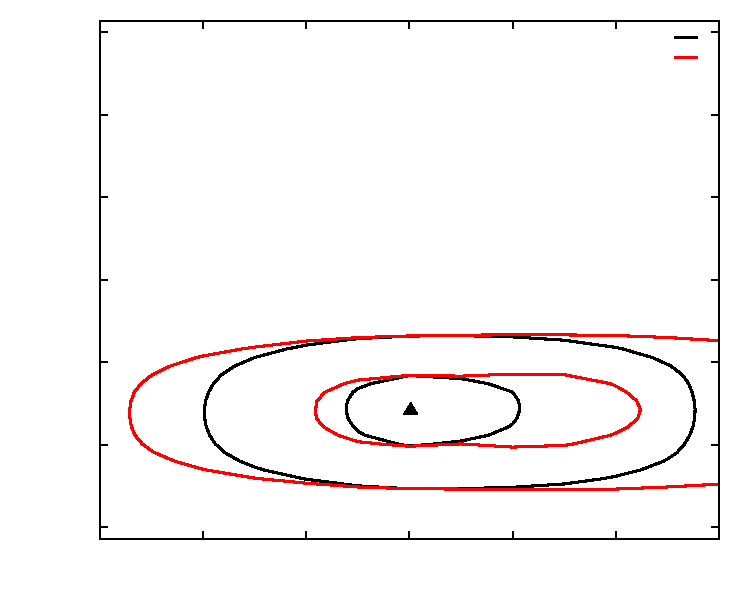
\includegraphics{pics/just0_cont_S13_dCP}}%
    \gplfronttext
  \end{picture}%
\endgroup
}	%%%%%%%%%%%this is important
	\caption[$\chi^2$ profiles for $\Delta m_{32}^2$, $\sin^2 2\theta_{13}$, and $\sin\theta_{23}$ with the nominal systematic model]%
		{$\chi^2$ profile for $\delta_\text{CP}$ (top left), $\sin^2 2\theta_{13}$ (top right), %
		$\Delta m_{32}^2$ (middle left), and $\sin^2 \theta_{23}$ (middle right), %
		together with the contour levels for $\delta_\text{CP}$ versus $\sin^2 2\theta_{13}$ (bottom left) %
		and $\Delta m_{32}^2$ versus $\sin^2 \theta_{23}$ (bottom right).
		The bottom panels in the top four figures show the difference between the $\chi^2$ profiles computed %
		with the penalty term and the $\chi^2$ profiles computed without.
		The dashed lines and the black triangles show the position of the best fit value, %
		which is always at the nominal Asimov A value.}
	\label{fig:nominal_profile}
\end{figure}


\begin{figure}
	\centering
	\resizebox{0.49\linewidth}{!}{% GNUPLOT: LaTeX picture with Postscript
\begingroup
  \makeatletter
  \providecommand\color[2][]{%
    \GenericError{(gnuplot) \space\space\space\@spaces}{%
      Package color not loaded in conjunction with
      terminal option `colourtext'%
    }{See the gnuplot documentation for explanation.%
    }{Either use 'blacktext' in gnuplot or load the package
      color.sty in LaTeX.}%
    \renewcommand\color[2][]{}%
  }%
  \providecommand\includegraphics[2][]{%
    \GenericError{(gnuplot) \space\space\space\@spaces}{%
      Package graphicx or graphics not loaded%
    }{See the gnuplot documentation for explanation.%
    }{The gnuplot epslatex terminal needs graphicx.sty or graphics.sty.}%
    \renewcommand\includegraphics[2][]{}%
  }%
  \providecommand\rotatebox[2]{#2}%
  \@ifundefined{ifGPcolor}{%
    \newif\ifGPcolor
    \GPcolortrue
  }{}%
  \@ifundefined{ifGPblacktext}{%
    \newif\ifGPblacktext
    \GPblacktexttrue
  }{}%
  % define a \g@addto@macro without @ in the name:
  \let\gplgaddtomacro\g@addto@macro
  % define empty templates for all commands taking text:
  \gdef\gplbacktext{}%
  \gdef\gplfronttext{}%
  \makeatother
  \ifGPblacktext
    % no textcolor at all
    \def\colorrgb#1{}%
    \def\colorgray#1{}%
  \else
    % gray or color?
    \ifGPcolor
      \def\colorrgb#1{\color[rgb]{#1}}%
      \def\colorgray#1{\color[gray]{#1}}%
      \expandafter\def\csname LTw\endcsname{\color{white}}%
      \expandafter\def\csname LTb\endcsname{\color{black}}%
      \expandafter\def\csname LTa\endcsname{\color{black}}%
      \expandafter\def\csname LT0\endcsname{\color[rgb]{1,0,0}}%
      \expandafter\def\csname LT1\endcsname{\color[rgb]{0,1,0}}%
      \expandafter\def\csname LT2\endcsname{\color[rgb]{0,0,1}}%
      \expandafter\def\csname LT3\endcsname{\color[rgb]{1,0,1}}%
      \expandafter\def\csname LT4\endcsname{\color[rgb]{0,1,1}}%
      \expandafter\def\csname LT5\endcsname{\color[rgb]{1,1,0}}%
      \expandafter\def\csname LT6\endcsname{\color[rgb]{0,0,0}}%
      \expandafter\def\csname LT7\endcsname{\color[rgb]{1,0.3,0}}%
      \expandafter\def\csname LT8\endcsname{\color[rgb]{0.5,0.5,0.5}}%
    \else
      % gray
      \def\colorrgb#1{\color{black}}%
      \def\colorgray#1{\color[gray]{#1}}%
      \expandafter\def\csname LTw\endcsname{\color{white}}%
      \expandafter\def\csname LTb\endcsname{\color{black}}%
      \expandafter\def\csname LTa\endcsname{\color{black}}%
      \expandafter\def\csname LT0\endcsname{\color{black}}%
      \expandafter\def\csname LT1\endcsname{\color{black}}%
      \expandafter\def\csname LT2\endcsname{\color{black}}%
      \expandafter\def\csname LT3\endcsname{\color{black}}%
      \expandafter\def\csname LT4\endcsname{\color{black}}%
      \expandafter\def\csname LT5\endcsname{\color{black}}%
      \expandafter\def\csname LT6\endcsname{\color{black}}%
      \expandafter\def\csname LT7\endcsname{\color{black}}%
      \expandafter\def\csname LT8\endcsname{\color{black}}%
    \fi
  \fi
    \setlength{\unitlength}{0.0500bp}%
    \ifx\gptboxheight\undefined%
      \newlength{\gptboxheight}%
      \newlength{\gptboxwidth}%
      \newsavebox{\gptboxtext}%
    \fi%
    \setlength{\fboxrule}{0.5pt}%
    \setlength{\fboxsep}{1pt}%
\begin{picture}(7200.00,5040.00)%
    \gplgaddtomacro\gplbacktext{%
      \csname LTb\endcsname%%
      \put(441,595){\makebox(0,0)[r]{\strut{}0}}%
      \csname LTb\endcsname%%
      \put(441,1660){\makebox(0,0)[r]{\strut{}2}}%
      \csname LTb\endcsname%%
      \put(441,2724){\makebox(0,0)[r]{\strut{}4}}%
      \csname LTb\endcsname%%
      \put(441,3789){\makebox(0,0)[r]{\strut{}6}}%
      \csname LTb\endcsname%%
      \put(441,4853){\makebox(0,0)[r]{\strut{}8}}%
      \csname LTb\endcsname%%
      \put(543,409){\makebox(0,0){\strut{}-1.0$\pi$}}%
      \csname LTb\endcsname%%
      \put(1337,409){\makebox(0,0){\strut{}-0.8$\pi$}}%
      \csname LTb\endcsname%%
      \put(2131,409){\makebox(0,0){\strut{}-0.5$\pi$}}%
      \csname LTb\endcsname%%
      \put(2924,409){\makebox(0,0){\strut{}-0.2$\pi$}}%
      \csname LTb\endcsname%%
      \put(3718,409){\makebox(0,0){\strut{}0.0$\pi$}}%
      \csname LTb\endcsname%%
      \put(4512,409){\makebox(0,0){\strut{}0.2$\pi$}}%
      \csname LTb\endcsname%%
      \put(5306,409){\makebox(0,0){\strut{}0.5$\pi$}}%
      \csname LTb\endcsname%%
      \put(6099,409){\makebox(0,0){\strut{}0.8$\pi$}}%
      \csname LTb\endcsname%%
      \put(6893,409){\makebox(0,0){\strut{}1.0$\pi$}}%
      \csname LTb\endcsname%%
      \put(3718,3522){\makebox(0,0){\strut{}$5 \sigma$}}%
      \csname LTb\endcsname%%
      \put(3718,2458){\makebox(0,0){\strut{}$3 \sigma$}}%
    }%
    \gplgaddtomacro\gplfronttext{%
      \csname LTb\endcsname%%
      \put(153,2724){\rotatebox{-270}{\makebox(0,0){\strut{}$\sigma (\delta_\text{CP})$}}}%
      \csname LTb\endcsname%%
      \put(3718,130){\makebox(0,0){\strut{}$\delta_\text{CP}$}}%
      \csname LTb\endcsname%%
      \put(1076,4686){\makebox(0,0)[l]{\strut{}w/ penalty}}%
      \csname LTb\endcsname%%
      \put(1076,4500){\makebox(0,0)[l]{\strut{}w/o penalty}}%
    }%
    \gplbacktext
    \put(0,0){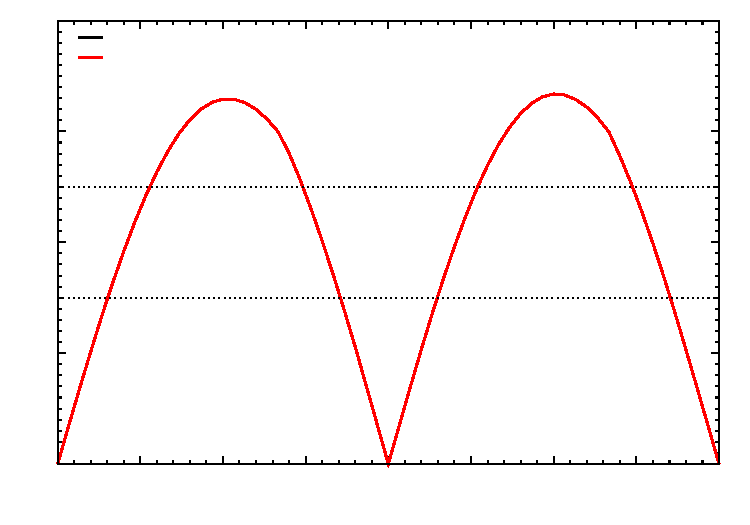
\includegraphics{pics/just0_sensitivity}}%
    \gplfronttext
  \end{picture}%
\endgroup
}
	\resizebox{0.49\linewidth}{!}{% GNUPLOT: LaTeX picture with Postscript
\begingroup
  \makeatletter
  \providecommand\color[2][]{%
    \GenericError{(gnuplot) \space\space\space\@spaces}{%
      Package color not loaded in conjunction with
      terminal option `colourtext'%
    }{See the gnuplot documentation for explanation.%
    }{Either use 'blacktext' in gnuplot or load the package
      color.sty in LaTeX.}%
    \renewcommand\color[2][]{}%
  }%
  \providecommand\includegraphics[2][]{%
    \GenericError{(gnuplot) \space\space\space\@spaces}{%
      Package graphicx or graphics not loaded%
    }{See the gnuplot documentation for explanation.%
    }{The gnuplot epslatex terminal needs graphicx.sty or graphics.sty.}%
    \renewcommand\includegraphics[2][]{}%
  }%
  \providecommand\rotatebox[2]{#2}%
  \@ifundefined{ifGPcolor}{%
    \newif\ifGPcolor
    \GPcolortrue
  }{}%
  \@ifundefined{ifGPblacktext}{%
    \newif\ifGPblacktext
    \GPblacktexttrue
  }{}%
  % define a \g@addto@macro without @ in the name:
  \let\gplgaddtomacro\g@addto@macro
  % define empty templates for all commands taking text:
  \gdef\gplbacktext{}%
  \gdef\gplfronttext{}%
  \makeatother
  \ifGPblacktext
    % no textcolor at all
    \def\colorrgb#1{}%
    \def\colorgray#1{}%
  \else
    % gray or color?
    \ifGPcolor
      \def\colorrgb#1{\color[rgb]{#1}}%
      \def\colorgray#1{\color[gray]{#1}}%
      \expandafter\def\csname LTw\endcsname{\color{white}}%
      \expandafter\def\csname LTb\endcsname{\color{black}}%
      \expandafter\def\csname LTa\endcsname{\color{black}}%
      \expandafter\def\csname LT0\endcsname{\color[rgb]{1,0,0}}%
      \expandafter\def\csname LT1\endcsname{\color[rgb]{0,1,0}}%
      \expandafter\def\csname LT2\endcsname{\color[rgb]{0,0,1}}%
      \expandafter\def\csname LT3\endcsname{\color[rgb]{1,0,1}}%
      \expandafter\def\csname LT4\endcsname{\color[rgb]{0,1,1}}%
      \expandafter\def\csname LT5\endcsname{\color[rgb]{1,1,0}}%
      \expandafter\def\csname LT6\endcsname{\color[rgb]{0,0,0}}%
      \expandafter\def\csname LT7\endcsname{\color[rgb]{1,0.3,0}}%
      \expandafter\def\csname LT8\endcsname{\color[rgb]{0.5,0.5,0.5}}%
    \else
      % gray
      \def\colorrgb#1{\color{black}}%
      \def\colorgray#1{\color[gray]{#1}}%
      \expandafter\def\csname LTw\endcsname{\color{white}}%
      \expandafter\def\csname LTb\endcsname{\color{black}}%
      \expandafter\def\csname LTa\endcsname{\color{black}}%
      \expandafter\def\csname LT0\endcsname{\color{black}}%
      \expandafter\def\csname LT1\endcsname{\color{black}}%
      \expandafter\def\csname LT2\endcsname{\color{black}}%
      \expandafter\def\csname LT3\endcsname{\color{black}}%
      \expandafter\def\csname LT4\endcsname{\color{black}}%
      \expandafter\def\csname LT5\endcsname{\color{black}}%
      \expandafter\def\csname LT6\endcsname{\color{black}}%
      \expandafter\def\csname LT7\endcsname{\color{black}}%
      \expandafter\def\csname LT8\endcsname{\color{black}}%
    \fi
  \fi
    \setlength{\unitlength}{0.0500bp}%
    \ifx\gptboxheight\undefined%
      \newlength{\gptboxheight}%
      \newlength{\gptboxwidth}%
      \newsavebox{\gptboxtext}%
    \fi%
    \setlength{\fboxrule}{0.5pt}%
    \setlength{\fboxsep}{1pt}%
\begin{picture}(7200.00,5040.00)%
    \gplgaddtomacro\gplbacktext{%
      \csname LTb\endcsname%%
      \put(441,595){\makebox(0,0)[r]{\strut{}0}}%
      \csname LTb\endcsname%%
      \put(441,1660){\makebox(0,0)[r]{\strut{}2}}%
      \csname LTb\endcsname%%
      \put(441,2724){\makebox(0,0)[r]{\strut{}4}}%
      \csname LTb\endcsname%%
      \put(441,3789){\makebox(0,0)[r]{\strut{}6}}%
      \csname LTb\endcsname%%
      \put(441,4853){\makebox(0,0)[r]{\strut{}8}}%
      \csname LTb\endcsname%%
      \put(543,409){\makebox(0,0){\strut{}-1.0$\pi$}}%
      \csname LTb\endcsname%%
      \put(1337,409){\makebox(0,0){\strut{}-0.8$\pi$}}%
      \csname LTb\endcsname%%
      \put(2131,409){\makebox(0,0){\strut{}-0.5$\pi$}}%
      \csname LTb\endcsname%%
      \put(2924,409){\makebox(0,0){\strut{}-0.2$\pi$}}%
      \csname LTb\endcsname%%
      \put(3718,409){\makebox(0,0){\strut{}0.0$\pi$}}%
      \csname LTb\endcsname%%
      \put(4512,409){\makebox(0,0){\strut{}0.2$\pi$}}%
      \csname LTb\endcsname%%
      \put(5306,409){\makebox(0,0){\strut{}0.5$\pi$}}%
      \csname LTb\endcsname%%
      \put(6099,409){\makebox(0,0){\strut{}0.8$\pi$}}%
      \csname LTb\endcsname%%
      \put(6893,409){\makebox(0,0){\strut{}1.0$\pi$}}%
      \csname LTb\endcsname%%
      \put(3718,3522){\makebox(0,0){\strut{}$5 \sigma$}}%
      \csname LTb\endcsname%%
      \put(3718,2458){\makebox(0,0){\strut{}$3 \sigma$}}%
    }%
    \gplgaddtomacro\gplfronttext{%
      \csname LTb\endcsname%%
      \put(153,2724){\rotatebox{-270}{\makebox(0,0){\strut{}$\sigma (\delta_\text{CP})$}}}%
      \csname LTb\endcsname%%
      \put(3718,130){\makebox(0,0){\strut{}$\delta_\text{CP}$}}%
      \csname LTb\endcsname%%
      \put(1076,4686){\makebox(0,0)[l]{\strut{}100\,\% data}}%
      \csname LTb\endcsname%%
      \put(1076,4500){\makebox(0,0)[l]{\strut{}75\,\% data}}%
      \csname LTb\endcsname%%
      \put(1076,4314){\makebox(0,0)[l]{\strut{}50\,\% data}}%
      \csname LTb\endcsname%%
      \put(1076,4128){\makebox(0,0)[l]{\strut{}25\,\% data}}%
    }%
    \gplbacktext
    \put(0,0){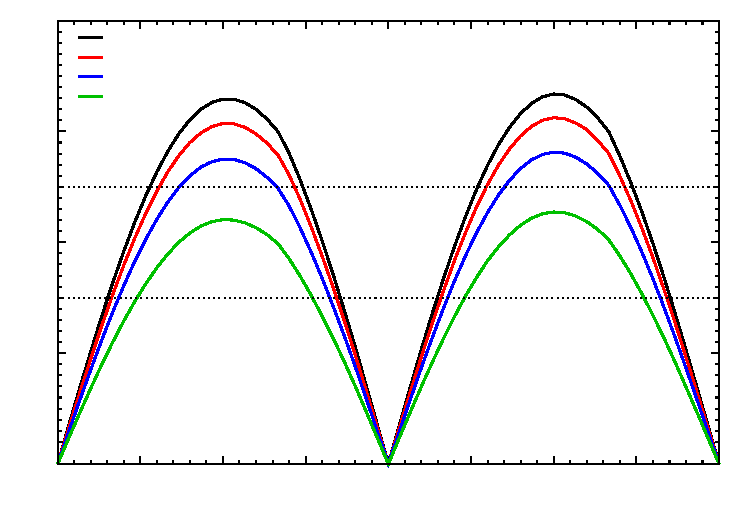
\includegraphics{pics/stats0_sensitivity}}%
    \gplfronttext
  \end{picture}%
\endgroup
}
	\caption[Sensitivity to $\delta_\text{CP}$ with the nominal systematic model]%
		{Expected significance to exclude CP conservation with the nominal model (left), %
		revealing that the sensitivity it is not affected by the penalty term of $\theta_{13}$ %
		from reactor constraints.
		On the right, the sensitivity to CP violation with full statistics (black) is compared %
		to different amounts of collected data: %
		with 25\,\% (green), 50\,\% (blue), and 75\,\% (red) of the total statistics.}
	\label{fig:nominal_sensitivity}
\end{figure}


The sensitivity to exclude CP conservation computed with the nominal systematic model %
is shown in \reffig{fig:nominal_sensitivity}.
The effect of the Gaussian penalty term does not impact the sensitivity of HK to CP violation, and %
therefore this term is always included in the following studies.
In \reffig{fig:nominal_sensitivity}, the sensitivity is shown at different stages of the experiment.
The effect is simulated by using rescaled event samples.
With only a quarter of the data collected, a maximally violating CP phase could be found with a significance of $3\sigma$, %
but with half of the statistics $5\sigma$ are easily reached.
Increasing the collected samples, the sensitivity quickly saturates to the best exclusion of $\sim6.5\sigma$.

\begin{figure}
	\centering
	\resizebox{0.7\linewidth}{!}{% GNUPLOT: LaTeX picture with Postscript
\begingroup
  \makeatletter
  \providecommand\color[2][]{%
    \GenericError{(gnuplot) \space\space\space\@spaces}{%
      Package color not loaded in conjunction with
      terminal option `colourtext'%
    }{See the gnuplot documentation for explanation.%
    }{Either use 'blacktext' in gnuplot or load the package
      color.sty in LaTeX.}%
    \renewcommand\color[2][]{}%
  }%
  \providecommand\includegraphics[2][]{%
    \GenericError{(gnuplot) \space\space\space\@spaces}{%
      Package graphicx or graphics not loaded%
    }{See the gnuplot documentation for explanation.%
    }{The gnuplot epslatex terminal needs graphicx.sty or graphics.sty.}%
    \renewcommand\includegraphics[2][]{}%
  }%
  \providecommand\rotatebox[2]{#2}%
  \@ifundefined{ifGPcolor}{%
    \newif\ifGPcolor
    \GPcolortrue
  }{}%
  \@ifundefined{ifGPblacktext}{%
    \newif\ifGPblacktext
    \GPblacktexttrue
  }{}%
  % define a \g@addto@macro without @ in the name:
  \let\gplgaddtomacro\g@addto@macro
  % define empty templates for all commands taking text:
  \gdef\gplbacktext{}%
  \gdef\gplfronttext{}%
  \makeatother
  \ifGPblacktext
    % no textcolor at all
    \def\colorrgb#1{}%
    \def\colorgray#1{}%
  \else
    % gray or color?
    \ifGPcolor
      \def\colorrgb#1{\color[rgb]{#1}}%
      \def\colorgray#1{\color[gray]{#1}}%
      \expandafter\def\csname LTw\endcsname{\color{white}}%
      \expandafter\def\csname LTb\endcsname{\color{black}}%
      \expandafter\def\csname LTa\endcsname{\color{black}}%
      \expandafter\def\csname LT0\endcsname{\color[rgb]{1,0,0}}%
      \expandafter\def\csname LT1\endcsname{\color[rgb]{0,1,0}}%
      \expandafter\def\csname LT2\endcsname{\color[rgb]{0,0,1}}%
      \expandafter\def\csname LT3\endcsname{\color[rgb]{1,0,1}}%
      \expandafter\def\csname LT4\endcsname{\color[rgb]{0,1,1}}%
      \expandafter\def\csname LT5\endcsname{\color[rgb]{1,1,0}}%
      \expandafter\def\csname LT6\endcsname{\color[rgb]{0,0,0}}%
      \expandafter\def\csname LT7\endcsname{\color[rgb]{1,0.3,0}}%
      \expandafter\def\csname LT8\endcsname{\color[rgb]{0.5,0.5,0.5}}%
    \else
      % gray
      \def\colorrgb#1{\color{black}}%
      \def\colorgray#1{\color[gray]{#1}}%
      \expandafter\def\csname LTw\endcsname{\color{white}}%
      \expandafter\def\csname LTb\endcsname{\color{black}}%
      \expandafter\def\csname LTa\endcsname{\color{black}}%
      \expandafter\def\csname LT0\endcsname{\color{black}}%
      \expandafter\def\csname LT1\endcsname{\color{black}}%
      \expandafter\def\csname LT2\endcsname{\color{black}}%
      \expandafter\def\csname LT3\endcsname{\color{black}}%
      \expandafter\def\csname LT4\endcsname{\color{black}}%
      \expandafter\def\csname LT5\endcsname{\color{black}}%
      \expandafter\def\csname LT6\endcsname{\color{black}}%
      \expandafter\def\csname LT7\endcsname{\color{black}}%
      \expandafter\def\csname LT8\endcsname{\color{black}}%
    \fi
  \fi
    \setlength{\unitlength}{0.0500bp}%
    \ifx\gptboxheight\undefined%
      \newlength{\gptboxheight}%
      \newlength{\gptboxwidth}%
      \newsavebox{\gptboxtext}%
    \fi%
    \setlength{\fboxrule}{0.5pt}%
    \setlength{\fboxsep}{1pt}%
\begin{picture}(8640.00,5760.00)%
    \gplgaddtomacro\gplbacktext{%
      \csname LTb\endcsname%%
      \put(441,595){\makebox(0,0)[r]{\strut{}0}}%
      \csname LTb\endcsname%%
      \put(441,1840){\makebox(0,0)[r]{\strut{}2}}%
      \csname LTb\endcsname%%
      \put(441,3084){\makebox(0,0)[r]{\strut{}4}}%
      \csname LTb\endcsname%%
      \put(441,4329){\makebox(0,0)[r]{\strut{}6}}%
      \csname LTb\endcsname%%
      \put(441,5573){\makebox(0,0)[r]{\strut{}8}}%
      \csname LTb\endcsname%%
      \put(543,409){\makebox(0,0){\strut{}-1.0$\pi$}}%
      \csname LTb\endcsname%%
      \put(1517,409){\makebox(0,0){\strut{}-0.8$\pi$}}%
      \csname LTb\endcsname%%
      \put(2491,409){\makebox(0,0){\strut{}-0.5$\pi$}}%
      \csname LTb\endcsname%%
      \put(3464,409){\makebox(0,0){\strut{}-0.2$\pi$}}%
      \csname LTb\endcsname%%
      \put(4438,409){\makebox(0,0){\strut{}0.0$\pi$}}%
      \csname LTb\endcsname%%
      \put(5412,409){\makebox(0,0){\strut{}0.2$\pi$}}%
      \csname LTb\endcsname%%
      \put(6386,409){\makebox(0,0){\strut{}0.5$\pi$}}%
      \csname LTb\endcsname%%
      \put(7359,409){\makebox(0,0){\strut{}0.8$\pi$}}%
      \csname LTb\endcsname%%
      \put(8333,409){\makebox(0,0){\strut{}1.0$\pi$}}%
      \csname LTb\endcsname%%
      \put(4438,4017){\makebox(0,0){\strut{}$5 \sigma$}}%
      \csname LTb\endcsname%%
      \put(4438,2773){\makebox(0,0){\strut{}$3 \sigma$}}%
    }%
    \gplgaddtomacro\gplfronttext{%
      \csname LTb\endcsname%%
      \put(153,3084){\rotatebox{-270}{\makebox(0,0){\strut{}$\sigma (\delta_\text{CP})$}}}%
      \csname LTb\endcsname%%
      \put(4438,130){\makebox(0,0){\strut{}$\delta_\text{CP}$}}%
      \csname LTb\endcsname%%
      \put(1076,5406){\makebox(0,0)[l]{\strut{}Beam}}%
      \csname LTb\endcsname%%
      \put(1076,5220){\makebox(0,0)[l]{\strut{}Atmospheric}}%
      \csname LTb\endcsname%%
      \put(1076,5034){\makebox(0,0)[l]{\strut{}Combined}}%
    }%
    \gplbacktext
    \put(0,0){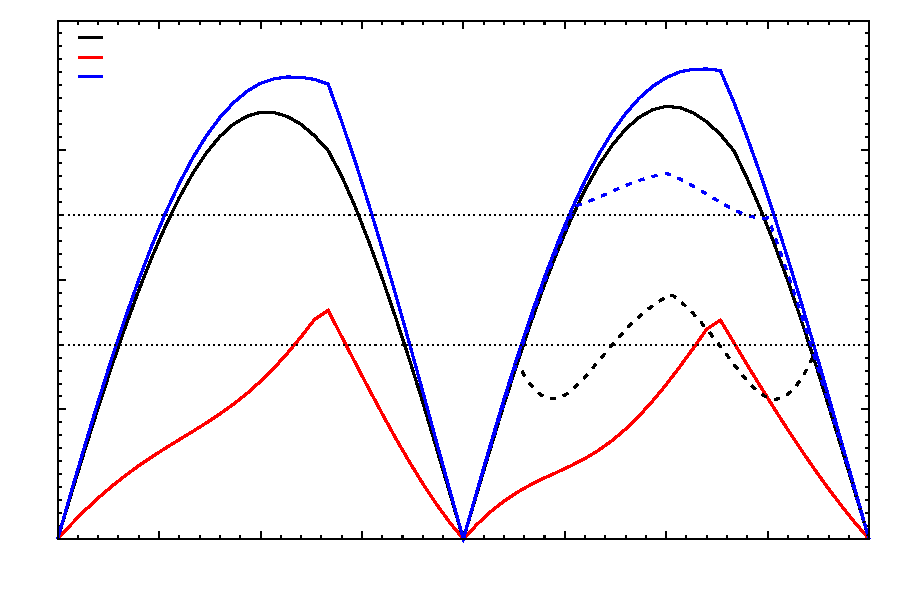
\includegraphics{pics/combined_sens}}%
    \gplfronttext
  \end{picture}%
\endgroup
}
	\caption[Sensitivity to $\delta_\text{CP}$ with the nominal model and unknown hierarchy]%
		{Expected significance to exclude CP conservation with the nominal model and %
		for the beam sample (black), the atmospheric sample (red) and the combination of the two (blue).
		The solid lines correspond to sensitivity where the mass hierarchy is known to be normal.
		If the mass hierarchy is not known the sensitivity is weakened.
		When the true mass ordering of the beam sample is normal and inverse hierarchy is fitted, %
		exclusion power is lost for $\delta_\text{CP} > 0$ (black dashed).
		Including the atmospheric sample in the fit restores partially the sensitivity (blue dashed).}
	\label{fig:combined_sens}
\end{figure}

The usefulness of performing a combined fit between beam and atmospheric %
data can be best understood from \reffig{fig:combined_sens}.
When the expected ($E_n$) and observed ($O_n$) event distributions are built for the $\chi^2$ calculation, %
a neutrino mass hierarchy must be assumed.
In reality, the true mass ordering is unknown and unless this freedom is parameterised in some way, %
it can happen that the wrong mass hierarchy is used in defining the expected events.
In this case, the sensitivity to certain values of $\delta_\text{CP}$ can deteriorate.
For example, if the true mass ordering is normal hierarchy and inverted hierarchy is assumed in the fit, %
the sensitivity for $\delta_\text{CP} < 0$ remains unaffected, whereas the one for $\delta_\text{CP} > 0$ worsens.
The opposite occurs in the reverse situation.
Adding the atmospheric sample to the likelihood calculation allows to partially recover the exclusion power to CP conservation.
The very long baseline of atmospheric neutrinos amplifies matter effects, thanks to which the sensitivity %
of the experiment to mass ordering.
The differences between expected and observed events thus intensify leading to larger values of the $\chi^2$.


\subsection{Variations of the nominal model}
\label{sec:variations}


Previous studies~\cite{Abe:2018wpn} found that some systematic uncertainties %
were not easily implemented by varying model parameters.
These were then the subjects of fake data studies, where a variant systematic model was analysed under %
the assumptions of the default model.
A series of modifications of the nominal systematic model are performed also for this study.
New systematic sets are created, and by performing sensitivity studies with these variations of the nominal model %
it is possible to determine whether certain systematic errors need more control than other.
All of the produced sets are listed in \reftab{tab:variations}, even though only %
some of them have been analysed in this thesis and these are:
increment of the $\nu_e$ flux uncertainty in the $\nu$-mode beam by 2\%, labelled \textbf{8}; %
increment of the energy scale uncertainty, from 2.4\,\% to 2.9\,\%, labelled \textbf{11a}; %
decrement of the energy scale uncertainty, from 2.4\,\% to 1.9\,\%, labelled \textbf{11b}.
The remaining ones will be analysed in future studies.
The new three profiles are shown collectively with the nominal model, labelled \textbf{0}, in \reffig{fig:0_11a_11b_8_profile}.
The $\chi^2$ as a function of $\delta_\text{CP}$ and $\sin^2 2\theta_{13}$ changes slightly with a different flux uncertainty, %
but it is not very much affected by a variation of the energy scale error.
The opposite is true for $\chi^2$ versus $\Delta m_{32}^2$ or $\sin^2\theta_{23}$, in which %
varying the energy scale error is reflected in larger deviations from the nominal model away from the best fit value.
The contour plots in \reffig{fig:0_11a_11b_8_profile} confirm that no appreciable deviation from the nominal model %
is seen for $\chi^2$ levels corresponding to $1\sigma$ and $3\sigma$.
In terms of sensitivity, the variation induced by the modified systematic model is %
less than 0.1\,\% at values of maximal violation of CP, as it can be appreciated in \reffig{fig:0_11a_11b_8_sensitivity}.
The treatment of the energy scale uncertainty with the methodology described in this chapter might be too simplistic.
The linear behaviour of the systematic errors (see \refeq{eq:linear}) should be applied with mindfulness: %
it follows that the systematic parameters in the $\chi^2$ can commute with each other; %
the energy scale error, however, does not since it effectively shifts the bin contents of the event distributions.
It is also believed that this parameter is simultaneously constrained by the $e$-like samples %
the $\mu$-like samples, thus exhibiting no appreciable effect on the sensitivity prediction.
There is probably need to improve the systematic model by not only duplicating the energy scale systematic %
between the two data samples, but also by changing the $\chi^2$ definition and the way this parameter is treated.

Keeping in mind the above caveats, the sensitivity to $\delta_\text{CP}$ from \reffig{fig:0_11a_11b_8_sensitivity} %
is above $6\sigma$ at full statistics.
It is expected that the systematics variations of \reftab{tab:variations} should not degrade %
the significance of CP conservation exclusion below this value.
Further studies are in place before the definitive quantitative results, %
since a more accurate treatment of the energy scale parameter is needed.
Once the beam sample is extensively analysed, the atmospheric sample can be added to the $\chi^2$ calculation %
and a more complicated and comprehensive systematic model can be adopted. 

\begin{table}
	\centering
	\caption[Variations of the nominal systematic model]%
		{Variations of the nominal systematic model, labelled \textbf{0}.
		The second column specify the modification applied to the reference model:
		the sets in the first block have one or more parameters added, %
		whereas one or more parameters are removed in the variations of the second block.
		The systematic models in the last group have the same number of parameters of the nominal model, %
		with the modifications specified.}
	\label{tab:variations}
	\small
	\begin{tabular}{rr@{\quad}l}
		\toprule
		%Label		& & Modification \\
		%\midrule
		\textbf{0}	& 	& Nominal T2K model \\
		\midrule
		\textbf{1a}	& $=\quad\bs{0}\quad+$ 	& $\nu_e$ CC cross-sections for $0.1\,\text{GeV} < E_\text{true} < 0.6\,\text{GeV}$ \\
		\textbf{1b}	& $=\quad\bs{0}\quad+$ 	& $\nu_e$ CC cross-sections for $0.6\,\text{GeV} < E_\text{true} < 1.0\,\text{GeV}$ \\
		\textbf{2a}	& $=\quad\bs{0}\quad+$ 	& $\cj{\nu}_e$ CC cross-sections for $0.1\,\text{GeV} < E_\text{true} < 0.6\,\text{GeV}$ \\
		\textbf{2b}	& $=\quad\bs{0}\quad+$ 	& $\cj{\nu}_e$ CC cross-sections for $0.6\,\text{GeV} < E_\text{true} < 1.0\,\text{GeV}$ \\
		\textbf{9}	& $=\quad\bs{0}\quad+$	& CC1$\pi^\pm$ and CC-coh cross-sections for $\nu_e$ and $\cj{\nu}_e$. \\
		\textbf{10}	& $=\quad\bs{0}\quad+$	& CC1$\pi^\pm$ and CC-coh cross-sections for $\nu_\mu$ and $\cj{\nu}_\mu$ \\
				&   			  & \hfill	for $2\,\text{GeV} < E_\text{true} < 10\,\text{GeV}$ \\
		\midrule
		\textbf{6a}	& $=\quad\bs{0}\quad-$	& $\nu$ 2p-2h normalisation \\
		\textbf{7a}	& $=\quad\bs{0}\quad-$	& $\cj{\nu}$ 2p-2h normalisation \\
		\textbf{67}	& $=\quad\bs{0}\quad-$	& $\nu$ and $\cj{\nu}$ 2p-2h normalisation \\
		\midrule
		\textbf{8}	& $=\quad\bs{0}\quad\times$	& increased $\nu_e$ flux uncertainty in $\nu$-mode beam (2\%) \\
		\textbf{11a}	& $=\quad\bs{0}\quad\times$	& increased energy scale (2.4\% $\to$ 2.9\%) \\
		\textbf{11b}	& $=\quad\bs{0}\quad\times$	& decreased energy scale (2.4\% $\to$ 1.9\%) \\
		\textbf{flux}	& $=\quad\bs{0}\quad\times$	& flux model additions from INGRID studies \\
		\bottomrule
	\end{tabular}
\end{table}

\begin{figure}
	\centering
	\resizebox{0.49\linewidth}{!}{% GNUPLOT: LaTeX picture with Postscript
\begingroup
  \makeatletter
  \providecommand\color[2][]{%
    \GenericError{(gnuplot) \space\space\space\@spaces}{%
      Package color not loaded in conjunction with
      terminal option `colourtext'%
    }{See the gnuplot documentation for explanation.%
    }{Either use 'blacktext' in gnuplot or load the package
      color.sty in LaTeX.}%
    \renewcommand\color[2][]{}%
  }%
  \providecommand\includegraphics[2][]{%
    \GenericError{(gnuplot) \space\space\space\@spaces}{%
      Package graphicx or graphics not loaded%
    }{See the gnuplot documentation for explanation.%
    }{The gnuplot epslatex terminal needs graphicx.sty or graphics.sty.}%
    \renewcommand\includegraphics[2][]{}%
  }%
  \providecommand\rotatebox[2]{#2}%
  \@ifundefined{ifGPcolor}{%
    \newif\ifGPcolor
    \GPcolortrue
  }{}%
  \@ifundefined{ifGPblacktext}{%
    \newif\ifGPblacktext
    \GPblacktexttrue
  }{}%
  % define a \g@addto@macro without @ in the name:
  \let\gplgaddtomacro\g@addto@macro
  % define empty templates for all commands taking text:
  \gdef\gplbacktext{}%
  \gdef\gplfronttext{}%
  \makeatother
  \ifGPblacktext
    % no textcolor at all
    \def\colorrgb#1{}%
    \def\colorgray#1{}%
  \else
    % gray or color?
    \ifGPcolor
      \def\colorrgb#1{\color[rgb]{#1}}%
      \def\colorgray#1{\color[gray]{#1}}%
      \expandafter\def\csname LTw\endcsname{\color{white}}%
      \expandafter\def\csname LTb\endcsname{\color{black}}%
      \expandafter\def\csname LTa\endcsname{\color{black}}%
      \expandafter\def\csname LT0\endcsname{\color[rgb]{1,0,0}}%
      \expandafter\def\csname LT1\endcsname{\color[rgb]{0,1,0}}%
      \expandafter\def\csname LT2\endcsname{\color[rgb]{0,0,1}}%
      \expandafter\def\csname LT3\endcsname{\color[rgb]{1,0,1}}%
      \expandafter\def\csname LT4\endcsname{\color[rgb]{0,1,1}}%
      \expandafter\def\csname LT5\endcsname{\color[rgb]{1,1,0}}%
      \expandafter\def\csname LT6\endcsname{\color[rgb]{0,0,0}}%
      \expandafter\def\csname LT7\endcsname{\color[rgb]{1,0.3,0}}%
      \expandafter\def\csname LT8\endcsname{\color[rgb]{0.5,0.5,0.5}}%
    \else
      % gray
      \def\colorrgb#1{\color{black}}%
      \def\colorgray#1{\color[gray]{#1}}%
      \expandafter\def\csname LTw\endcsname{\color{white}}%
      \expandafter\def\csname LTb\endcsname{\color{black}}%
      \expandafter\def\csname LTa\endcsname{\color{black}}%
      \expandafter\def\csname LT0\endcsname{\color{black}}%
      \expandafter\def\csname LT1\endcsname{\color{black}}%
      \expandafter\def\csname LT2\endcsname{\color{black}}%
      \expandafter\def\csname LT3\endcsname{\color{black}}%
      \expandafter\def\csname LT4\endcsname{\color{black}}%
      \expandafter\def\csname LT5\endcsname{\color{black}}%
      \expandafter\def\csname LT6\endcsname{\color{black}}%
      \expandafter\def\csname LT7\endcsname{\color{black}}%
      \expandafter\def\csname LT8\endcsname{\color{black}}%
    \fi
  \fi
    \setlength{\unitlength}{0.0500bp}%
    \ifx\gptboxheight\undefined%
      \newlength{\gptboxheight}%
      \newlength{\gptboxwidth}%
      \newsavebox{\gptboxtext}%
    \fi%
    \setlength{\fboxrule}{0.5pt}%
    \setlength{\fboxsep}{1pt}%
\begin{picture}(7200.00,5760.00)%
    \gplgaddtomacro\gplbacktext{%
      \csname LTb\endcsname%%
      \put(618,864){\makebox(0,0)[r]{\strut{}-0.3}}%
      \csname LTb\endcsname%%
      \put(618,1368){\makebox(0,0)[r]{\strut{}-0.2}}%
      \csname LTb\endcsname%%
      \put(618,1872){\makebox(0,0)[r]{\strut{}-0.1}}%
      \csname LTb\endcsname%%
      \put(618,2376){\makebox(0,0)[r]{\strut{}0}}%
      \csname LTb\endcsname%%
      \put(720,678){\makebox(0,0){\strut{}-1.00$\pi$}}%
      \csname LTb\endcsname%%
      \put(1524,678){\makebox(0,0){\strut{}-0.75$\pi$}}%
      \csname LTb\endcsname%%
      \put(2327,678){\makebox(0,0){\strut{}-0.50$\pi$}}%
      \csname LTb\endcsname%%
      \put(3131,678){\makebox(0,0){\strut{}-0.25$\pi$}}%
      \csname LTb\endcsname%%
      \put(3934,678){\makebox(0,0){\strut{}0.00$\pi$}}%
      \csname LTb\endcsname%%
      \put(4738,678){\makebox(0,0){\strut{}0.25$\pi$}}%
      \csname LTb\endcsname%%
      \put(5541,678){\makebox(0,0){\strut{}0.50$\pi$}}%
      \csname LTb\endcsname%%
      \put(6345,678){\makebox(0,0){\strut{}0.75$\pi$}}%
      \csname LTb\endcsname%%
      \put(7148,678){\makebox(0,0){\strut{}1.00$\pi$}}%
    }%
    \gplgaddtomacro\gplfronttext{%
      \csname LTb\endcsname%%
      \put(24,1872){\rotatebox{-270}{\makebox(0,0){\strut{}$\Delta \chi^2_0 - \Delta \chi^2$}}}%
      \csname LTb\endcsname%%
      \put(3934,399){\makebox(0,0){\strut{}$\delta_\text{CP}$}}%
    }%
    \gplgaddtomacro\gplbacktext{%
      \csname LTb\endcsname%%
      \put(618,2880){\makebox(0,0)[r]{\strut{}0}}%
      \csname LTb\endcsname%%
      \put(618,3499){\makebox(0,0)[r]{\strut{}40}}%
      \csname LTb\endcsname%%
      \put(618,4118){\makebox(0,0)[r]{\strut{}80}}%
      \csname LTb\endcsname%%
      \put(618,4737){\makebox(0,0)[r]{\strut{}120}}%
      \csname LTb\endcsname%%
      \put(618,5356){\makebox(0,0)[r]{\strut{}160}}%
      \csname LTb\endcsname%%
      \put(720,2694){\makebox(0,0){\strut{}}}%
      \csname LTb\endcsname%%
      \put(1524,2694){\makebox(0,0){\strut{}}}%
      \csname LTb\endcsname%%
      \put(2327,2694){\makebox(0,0){\strut{}}}%
      \csname LTb\endcsname%%
      \put(3131,2694){\makebox(0,0){\strut{}}}%
      \csname LTb\endcsname%%
      \put(3934,2694){\makebox(0,0){\strut{}}}%
      \csname LTb\endcsname%%
      \put(4738,2694){\makebox(0,0){\strut{}}}%
      \csname LTb\endcsname%%
      \put(5541,2694){\makebox(0,0){\strut{}}}%
      \csname LTb\endcsname%%
      \put(6345,2694){\makebox(0,0){\strut{}}}%
      \csname LTb\endcsname%%
      \put(7148,2694){\makebox(0,0){\strut{}}}%
    }%
    \gplgaddtomacro\gplfronttext{%
      \csname LTb\endcsname%%
      \put(126,4273){\rotatebox{-270}{\makebox(0,0){\strut{}$\Delta \chi^2$}}}%
      \csname LTb\endcsname%%
      \put(3934,2638){\makebox(0,0){\strut{}}}%
      \csname LTb\endcsname%%
      \put(2977,4877){\makebox(0,0){\strut{}}}%
      \csname LTb\endcsname%%
      \put(3068,4877){\makebox(0,0)[r]{\strut{}0}}%
      \csname LTb\endcsname%%
      \put(3068,4691){\makebox(0,0)[r]{\strut{}11a}}%
      \csname LTb\endcsname%%
      \put(3068,4505){\makebox(0,0)[r]{\strut{}11b}}%
      \csname LTb\endcsname%%
      \put(3068,4319){\makebox(0,0)[r]{\strut{}8}}%
    }%
    \gplbacktext
    \put(0,0){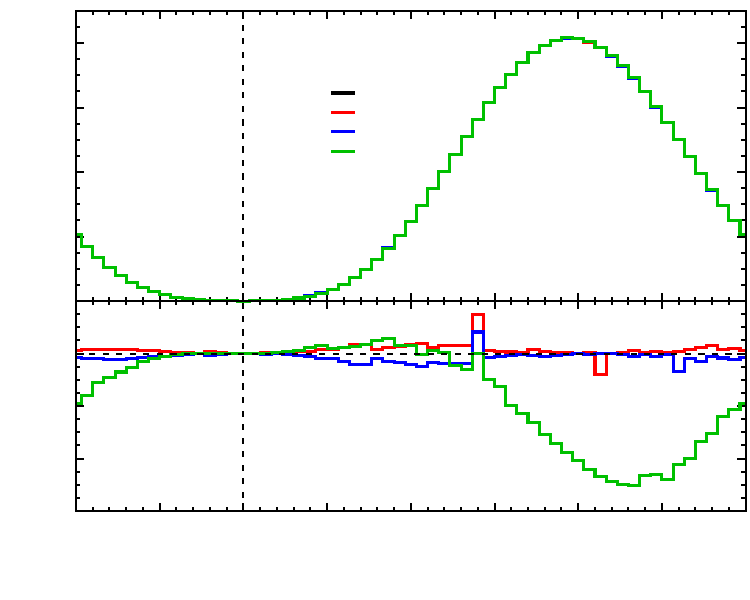
\includegraphics{pics/new_0_11a_11b_8_chi2_dCP}}%
    \gplfronttext
  \end{picture}%
\endgroup
}
	\resizebox{0.49\linewidth}{!}{% GNUPLOT: LaTeX picture with Postscript
\begingroup
  \makeatletter
  \providecommand\color[2][]{%
    \GenericError{(gnuplot) \space\space\space\@spaces}{%
      Package color not loaded in conjunction with
      terminal option `colourtext'%
    }{See the gnuplot documentation for explanation.%
    }{Either use 'blacktext' in gnuplot or load the package
      color.sty in LaTeX.}%
    \renewcommand\color[2][]{}%
  }%
  \providecommand\includegraphics[2][]{%
    \GenericError{(gnuplot) \space\space\space\@spaces}{%
      Package graphicx or graphics not loaded%
    }{See the gnuplot documentation for explanation.%
    }{The gnuplot epslatex terminal needs graphicx.sty or graphics.sty.}%
    \renewcommand\includegraphics[2][]{}%
  }%
  \providecommand\rotatebox[2]{#2}%
  \@ifundefined{ifGPcolor}{%
    \newif\ifGPcolor
    \GPcolortrue
  }{}%
  \@ifundefined{ifGPblacktext}{%
    \newif\ifGPblacktext
    \GPblacktexttrue
  }{}%
  % define a \g@addto@macro without @ in the name:
  \let\gplgaddtomacro\g@addto@macro
  % define empty templates for all commands taking text:
  \gdef\gplbacktext{}%
  \gdef\gplfronttext{}%
  \makeatother
  \ifGPblacktext
    % no textcolor at all
    \def\colorrgb#1{}%
    \def\colorgray#1{}%
  \else
    % gray or color?
    \ifGPcolor
      \def\colorrgb#1{\color[rgb]{#1}}%
      \def\colorgray#1{\color[gray]{#1}}%
      \expandafter\def\csname LTw\endcsname{\color{white}}%
      \expandafter\def\csname LTb\endcsname{\color{black}}%
      \expandafter\def\csname LTa\endcsname{\color{black}}%
      \expandafter\def\csname LT0\endcsname{\color[rgb]{1,0,0}}%
      \expandafter\def\csname LT1\endcsname{\color[rgb]{0,1,0}}%
      \expandafter\def\csname LT2\endcsname{\color[rgb]{0,0,1}}%
      \expandafter\def\csname LT3\endcsname{\color[rgb]{1,0,1}}%
      \expandafter\def\csname LT4\endcsname{\color[rgb]{0,1,1}}%
      \expandafter\def\csname LT5\endcsname{\color[rgb]{1,1,0}}%
      \expandafter\def\csname LT6\endcsname{\color[rgb]{0,0,0}}%
      \expandafter\def\csname LT7\endcsname{\color[rgb]{1,0.3,0}}%
      \expandafter\def\csname LT8\endcsname{\color[rgb]{0.5,0.5,0.5}}%
    \else
      % gray
      \def\colorrgb#1{\color{black}}%
      \def\colorgray#1{\color[gray]{#1}}%
      \expandafter\def\csname LTw\endcsname{\color{white}}%
      \expandafter\def\csname LTb\endcsname{\color{black}}%
      \expandafter\def\csname LTa\endcsname{\color{black}}%
      \expandafter\def\csname LT0\endcsname{\color{black}}%
      \expandafter\def\csname LT1\endcsname{\color{black}}%
      \expandafter\def\csname LT2\endcsname{\color{black}}%
      \expandafter\def\csname LT3\endcsname{\color{black}}%
      \expandafter\def\csname LT4\endcsname{\color{black}}%
      \expandafter\def\csname LT5\endcsname{\color{black}}%
      \expandafter\def\csname LT6\endcsname{\color{black}}%
      \expandafter\def\csname LT7\endcsname{\color{black}}%
      \expandafter\def\csname LT8\endcsname{\color{black}}%
    \fi
  \fi
    \setlength{\unitlength}{0.0500bp}%
    \ifx\gptboxheight\undefined%
      \newlength{\gptboxheight}%
      \newlength{\gptboxwidth}%
      \newsavebox{\gptboxtext}%
    \fi%
    \setlength{\fboxrule}{0.5pt}%
    \setlength{\fboxsep}{1pt}%
\begin{picture}(7200.00,5760.00)%
    \gplgaddtomacro\gplbacktext{%
      \csname LTb\endcsname%%
      \put(618,864){\makebox(0,0)[r]{\strut{}-0.01}}%
      \csname LTb\endcsname%%
      \put(618,1440){\makebox(0,0)[r]{\strut{}0.01}}%
      \csname LTb\endcsname%%
      \put(618,2016){\makebox(0,0)[r]{\strut{}0.03}}%
      \csname LTb\endcsname%%
      \put(618,2592){\makebox(0,0)[r]{\strut{}0.05}}%
      \csname LTb\endcsname%%
      \put(720,678){\makebox(0,0){\strut{}0.07}}%
      \csname LTb\endcsname%%
      \put(1791,678){\makebox(0,0){\strut{}0.075}}%
      \csname LTb\endcsname%%
      \put(2863,678){\makebox(0,0){\strut{}0.08}}%
      \csname LTb\endcsname%%
      \put(3934,678){\makebox(0,0){\strut{}0.085}}%
      \csname LTb\endcsname%%
      \put(5005,678){\makebox(0,0){\strut{}0.09}}%
      \csname LTb\endcsname%%
      \put(6077,678){\makebox(0,0){\strut{}0.095}}%
      \csname LTb\endcsname%%
      \put(7148,678){\makebox(0,0){\strut{}0.1}}%
    }%
    \gplgaddtomacro\gplfronttext{%
      \csname LTb\endcsname%%
      \put(3934,399){\makebox(0,0){\strut{}$\sin^2 2 \theta_{13}$}}%
    }%
    \gplgaddtomacro\gplbacktext{%
      \csname LTb\endcsname%%
      \put(618,2880){\makebox(0,0)[r]{\strut{}0}}%
      \csname LTb\endcsname%%
      \put(618,3437){\makebox(0,0)[r]{\strut{}5}}%
      \csname LTb\endcsname%%
      \put(618,3994){\makebox(0,0)[r]{\strut{}10}}%
      \csname LTb\endcsname%%
      \put(618,4552){\makebox(0,0)[r]{\strut{}15}}%
      \csname LTb\endcsname%%
      \put(618,5109){\makebox(0,0)[r]{\strut{}20}}%
      \csname LTb\endcsname%%
      \put(618,5666){\makebox(0,0)[r]{\strut{}25}}%
      \csname LTb\endcsname%%
      \put(720,2694){\makebox(0,0){\strut{}}}%
      \csname LTb\endcsname%%
      \put(1791,2694){\makebox(0,0){\strut{}}}%
      \csname LTb\endcsname%%
      \put(2863,2694){\makebox(0,0){\strut{}}}%
      \csname LTb\endcsname%%
      \put(3934,2694){\makebox(0,0){\strut{}}}%
      \csname LTb\endcsname%%
      \put(5005,2694){\makebox(0,0){\strut{}}}%
      \csname LTb\endcsname%%
      \put(6077,2694){\makebox(0,0){\strut{}}}%
      \csname LTb\endcsname%%
      \put(7148,2694){\makebox(0,0){\strut{}}}%
    }%
    \gplgaddtomacro\gplfronttext{%
      \csname LTb\endcsname%%
      \put(228,4273){\rotatebox{-270}{\makebox(0,0){\strut{}$\Delta \chi^2$}}}%
      \csname LTb\endcsname%%
      \put(3934,2638){\makebox(0,0){\strut{}}}%
      \csname LTb\endcsname%%
      \put(4597,4877){\makebox(0,0){\strut{}}}%
      \csname LTb\endcsname%%
      \put(4688,4877){\makebox(0,0)[r]{\strut{}0}}%
      \csname LTb\endcsname%%
      \put(4688,4691){\makebox(0,0)[r]{\strut{}11a}}%
      \csname LTb\endcsname%%
      \put(4688,4505){\makebox(0,0)[r]{\strut{}11b}}%
      \csname LTb\endcsname%%
      \put(4688,4319){\makebox(0,0)[r]{\strut{}8}}%
    }%
    \gplbacktext
    \put(0,0){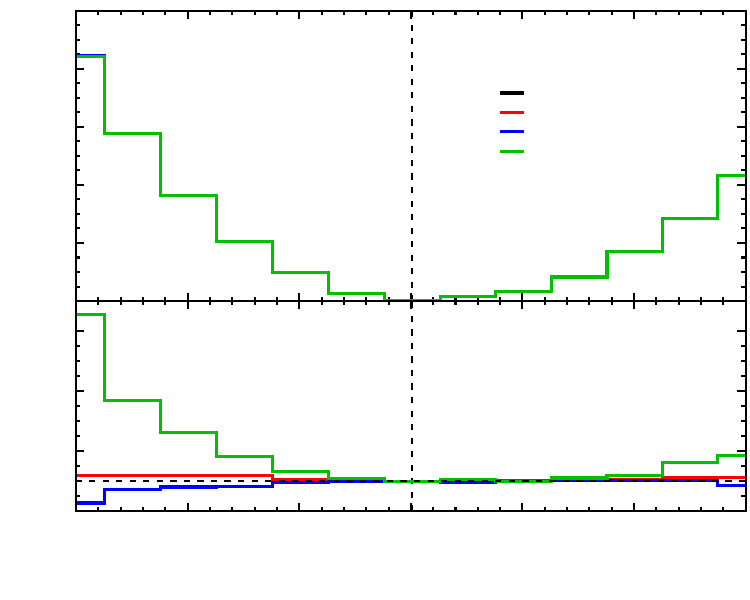
\includegraphics{pics/new_0_11a_11b_8_chi2_S13}}%
    \gplfronttext
  \end{picture}%
\endgroup
}
	\resizebox{0.49\linewidth}{!}{% GNUPLOT: LaTeX picture with Postscript
\begingroup
  \makeatletter
  \providecommand\color[2][]{%
    \GenericError{(gnuplot) \space\space\space\@spaces}{%
      Package color not loaded in conjunction with
      terminal option `colourtext'%
    }{See the gnuplot documentation for explanation.%
    }{Either use 'blacktext' in gnuplot or load the package
      color.sty in LaTeX.}%
    \renewcommand\color[2][]{}%
  }%
  \providecommand\includegraphics[2][]{%
    \GenericError{(gnuplot) \space\space\space\@spaces}{%
      Package graphicx or graphics not loaded%
    }{See the gnuplot documentation for explanation.%
    }{The gnuplot epslatex terminal needs graphicx.sty or graphics.sty.}%
    \renewcommand\includegraphics[2][]{}%
  }%
  \providecommand\rotatebox[2]{#2}%
  \@ifundefined{ifGPcolor}{%
    \newif\ifGPcolor
    \GPcolortrue
  }{}%
  \@ifundefined{ifGPblacktext}{%
    \newif\ifGPblacktext
    \GPblacktexttrue
  }{}%
  % define a \g@addto@macro without @ in the name:
  \let\gplgaddtomacro\g@addto@macro
  % define empty templates for all commands taking text:
  \gdef\gplbacktext{}%
  \gdef\gplfronttext{}%
  \makeatother
  \ifGPblacktext
    % no textcolor at all
    \def\colorrgb#1{}%
    \def\colorgray#1{}%
  \else
    % gray or color?
    \ifGPcolor
      \def\colorrgb#1{\color[rgb]{#1}}%
      \def\colorgray#1{\color[gray]{#1}}%
      \expandafter\def\csname LTw\endcsname{\color{white}}%
      \expandafter\def\csname LTb\endcsname{\color{black}}%
      \expandafter\def\csname LTa\endcsname{\color{black}}%
      \expandafter\def\csname LT0\endcsname{\color[rgb]{1,0,0}}%
      \expandafter\def\csname LT1\endcsname{\color[rgb]{0,1,0}}%
      \expandafter\def\csname LT2\endcsname{\color[rgb]{0,0,1}}%
      \expandafter\def\csname LT3\endcsname{\color[rgb]{1,0,1}}%
      \expandafter\def\csname LT4\endcsname{\color[rgb]{0,1,1}}%
      \expandafter\def\csname LT5\endcsname{\color[rgb]{1,1,0}}%
      \expandafter\def\csname LT6\endcsname{\color[rgb]{0,0,0}}%
      \expandafter\def\csname LT7\endcsname{\color[rgb]{1,0.3,0}}%
      \expandafter\def\csname LT8\endcsname{\color[rgb]{0.5,0.5,0.5}}%
    \else
      % gray
      \def\colorrgb#1{\color{black}}%
      \def\colorgray#1{\color[gray]{#1}}%
      \expandafter\def\csname LTw\endcsname{\color{white}}%
      \expandafter\def\csname LTb\endcsname{\color{black}}%
      \expandafter\def\csname LTa\endcsname{\color{black}}%
      \expandafter\def\csname LT0\endcsname{\color{black}}%
      \expandafter\def\csname LT1\endcsname{\color{black}}%
      \expandafter\def\csname LT2\endcsname{\color{black}}%
      \expandafter\def\csname LT3\endcsname{\color{black}}%
      \expandafter\def\csname LT4\endcsname{\color{black}}%
      \expandafter\def\csname LT5\endcsname{\color{black}}%
      \expandafter\def\csname LT6\endcsname{\color{black}}%
      \expandafter\def\csname LT7\endcsname{\color{black}}%
      \expandafter\def\csname LT8\endcsname{\color{black}}%
    \fi
  \fi
    \setlength{\unitlength}{0.0500bp}%
    \ifx\gptboxheight\undefined%
      \newlength{\gptboxheight}%
      \newlength{\gptboxwidth}%
      \newsavebox{\gptboxtext}%
    \fi%
    \setlength{\fboxrule}{0.5pt}%
    \setlength{\fboxsep}{1pt}%
\begin{picture}(7200.00,5760.00)%
    \gplgaddtomacro\gplbacktext{%
      \csname LTb\endcsname%%
      \put(618,864){\makebox(0,0)[r]{\strut{}-0.1}}%
      \csname LTb\endcsname%%
      \put(618,1872){\makebox(0,0)[r]{\strut{}0}}%
      \csname LTb\endcsname%%
      \put(720,678){\makebox(0,0){\strut{}2.464}}%
      \csname LTb\endcsname%%
      \put(1791,678){\makebox(0,0){\strut{}2.479}}%
      \csname LTb\endcsname%%
      \put(2863,678){\makebox(0,0){\strut{}2.494}}%
      \csname LTb\endcsname%%
      \put(3934,678){\makebox(0,0){\strut{}2.509}}%
      \csname LTb\endcsname%%
      \put(5005,678){\makebox(0,0){\strut{}2.524}}%
      \csname LTb\endcsname%%
      \put(6077,678){\makebox(0,0){\strut{}2.539}}%
      \csname LTb\endcsname%%
      \put(7148,678){\makebox(0,0){\strut{}2.554}}%
    }%
    \gplgaddtomacro\gplfronttext{%
      \csname LTb\endcsname%%
      \put(24,1872){\rotatebox{-270}{\makebox(0,0){\strut{}$\Delta \chi^2_0 - \Delta \chi^2$}}}%
      \csname LTb\endcsname%%
      \put(3934,399){\makebox(0,0){\strut{}$\Delta m_{32}^2 / 10^{-3}$}}%
    }%
    \gplgaddtomacro\gplbacktext{%
      \csname LTb\endcsname%%
      \put(618,2880){\makebox(0,0)[r]{\strut{}0}}%
      \csname LTb\endcsname%%
      \put(618,4273){\makebox(0,0)[r]{\strut{}5}}%
      \csname LTb\endcsname%%
      \put(618,5666){\makebox(0,0)[r]{\strut{}10}}%
      \csname LTb\endcsname%%
      \put(720,2694){\makebox(0,0){\strut{}}}%
      \csname LTb\endcsname%%
      \put(1791,2694){\makebox(0,0){\strut{}}}%
      \csname LTb\endcsname%%
      \put(2863,2694){\makebox(0,0){\strut{}}}%
      \csname LTb\endcsname%%
      \put(3934,2694){\makebox(0,0){\strut{}}}%
      \csname LTb\endcsname%%
      \put(5005,2694){\makebox(0,0){\strut{}}}%
      \csname LTb\endcsname%%
      \put(6077,2694){\makebox(0,0){\strut{}}}%
      \csname LTb\endcsname%%
      \put(7148,2694){\makebox(0,0){\strut{}}}%
    }%
    \gplgaddtomacro\gplfronttext{%
      \csname LTb\endcsname%%
      \put(228,4273){\rotatebox{-270}{\makebox(0,0){\strut{}$\Delta \chi^2$}}}%
      \csname LTb\endcsname%%
      \put(3934,2638){\makebox(0,0){\strut{}}}%
      \csname LTb\endcsname%%
      \put(4584,4877){\makebox(0,0){\strut{}}}%
      \csname LTb\endcsname%%
      \put(4675,4877){\makebox(0,0)[r]{\strut{}0}}%
      \csname LTb\endcsname%%
      \put(4675,4691){\makebox(0,0)[r]{\strut{}11a}}%
      \csname LTb\endcsname%%
      \put(4675,4505){\makebox(0,0)[r]{\strut{}11b}}%
      \csname LTb\endcsname%%
      \put(4675,4319){\makebox(0,0)[r]{\strut{}8}}%
    }%
    \gplbacktext
    \put(0,0){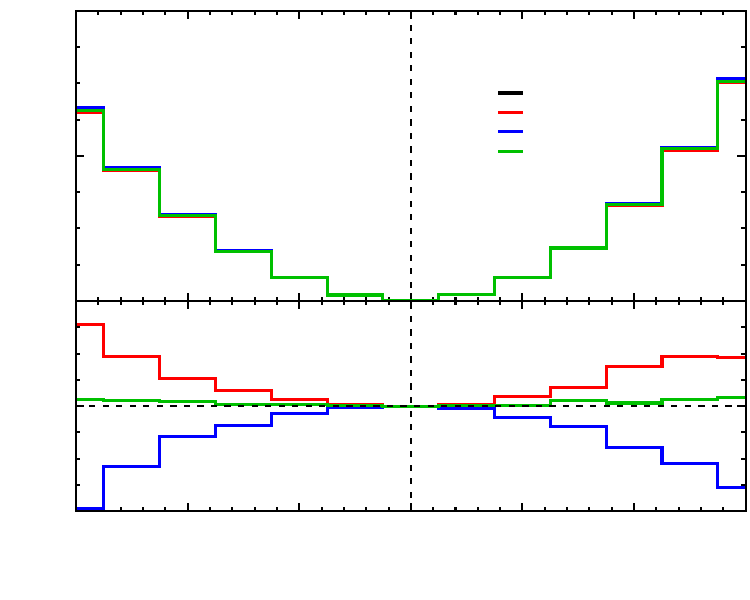
\includegraphics{pics/new_0_11a_11b_8_chi2_M23}}%
    \gplfronttext
  \end{picture}%
\endgroup
}
	\resizebox{0.49\linewidth}{!}{% GNUPLOT: LaTeX picture with Postscript
\begingroup
  \makeatletter
  \providecommand\color[2][]{%
    \GenericError{(gnuplot) \space\space\space\@spaces}{%
      Package color not loaded in conjunction with
      terminal option `colourtext'%
    }{See the gnuplot documentation for explanation.%
    }{Either use 'blacktext' in gnuplot or load the package
      color.sty in LaTeX.}%
    \renewcommand\color[2][]{}%
  }%
  \providecommand\includegraphics[2][]{%
    \GenericError{(gnuplot) \space\space\space\@spaces}{%
      Package graphicx or graphics not loaded%
    }{See the gnuplot documentation for explanation.%
    }{The gnuplot epslatex terminal needs graphicx.sty or graphics.sty.}%
    \renewcommand\includegraphics[2][]{}%
  }%
  \providecommand\rotatebox[2]{#2}%
  \@ifundefined{ifGPcolor}{%
    \newif\ifGPcolor
    \GPcolortrue
  }{}%
  \@ifundefined{ifGPblacktext}{%
    \newif\ifGPblacktext
    \GPblacktexttrue
  }{}%
  % define a \g@addto@macro without @ in the name:
  \let\gplgaddtomacro\g@addto@macro
  % define empty templates for all commands taking text:
  \gdef\gplbacktext{}%
  \gdef\gplfronttext{}%
  \makeatother
  \ifGPblacktext
    % no textcolor at all
    \def\colorrgb#1{}%
    \def\colorgray#1{}%
  \else
    % gray or color?
    \ifGPcolor
      \def\colorrgb#1{\color[rgb]{#1}}%
      \def\colorgray#1{\color[gray]{#1}}%
      \expandafter\def\csname LTw\endcsname{\color{white}}%
      \expandafter\def\csname LTb\endcsname{\color{black}}%
      \expandafter\def\csname LTa\endcsname{\color{black}}%
      \expandafter\def\csname LT0\endcsname{\color[rgb]{1,0,0}}%
      \expandafter\def\csname LT1\endcsname{\color[rgb]{0,1,0}}%
      \expandafter\def\csname LT2\endcsname{\color[rgb]{0,0,1}}%
      \expandafter\def\csname LT3\endcsname{\color[rgb]{1,0,1}}%
      \expandafter\def\csname LT4\endcsname{\color[rgb]{0,1,1}}%
      \expandafter\def\csname LT5\endcsname{\color[rgb]{1,1,0}}%
      \expandafter\def\csname LT6\endcsname{\color[rgb]{0,0,0}}%
      \expandafter\def\csname LT7\endcsname{\color[rgb]{1,0.3,0}}%
      \expandafter\def\csname LT8\endcsname{\color[rgb]{0.5,0.5,0.5}}%
    \else
      % gray
      \def\colorrgb#1{\color{black}}%
      \def\colorgray#1{\color[gray]{#1}}%
      \expandafter\def\csname LTw\endcsname{\color{white}}%
      \expandafter\def\csname LTb\endcsname{\color{black}}%
      \expandafter\def\csname LTa\endcsname{\color{black}}%
      \expandafter\def\csname LT0\endcsname{\color{black}}%
      \expandafter\def\csname LT1\endcsname{\color{black}}%
      \expandafter\def\csname LT2\endcsname{\color{black}}%
      \expandafter\def\csname LT3\endcsname{\color{black}}%
      \expandafter\def\csname LT4\endcsname{\color{black}}%
      \expandafter\def\csname LT5\endcsname{\color{black}}%
      \expandafter\def\csname LT6\endcsname{\color{black}}%
      \expandafter\def\csname LT7\endcsname{\color{black}}%
      \expandafter\def\csname LT8\endcsname{\color{black}}%
    \fi
  \fi
    \setlength{\unitlength}{0.0500bp}%
    \ifx\gptboxheight\undefined%
      \newlength{\gptboxheight}%
      \newlength{\gptboxwidth}%
      \newsavebox{\gptboxtext}%
    \fi%
    \setlength{\fboxrule}{0.5pt}%
    \setlength{\fboxsep}{1pt}%
\begin{picture}(7200.00,5760.00)%
    \gplgaddtomacro\gplbacktext{%
      \csname LTb\endcsname%%
      \put(618,864){\makebox(0,0)[r]{\strut{}-0.1}}%
      \csname LTb\endcsname%%
      \put(618,1536){\makebox(0,0)[r]{\strut{}0}}%
      \csname LTb\endcsname%%
      \put(618,2208){\makebox(0,0)[r]{\strut{}0.1}}%
      \csname LTb\endcsname%%
      \put(720,678){\makebox(0,0){\strut{}0.426}}%
      \csname LTb\endcsname%%
      \put(1791,678){\makebox(0,0){\strut{}0.4515}}%
      \csname LTb\endcsname%%
      \put(2863,678){\makebox(0,0){\strut{}0.477}}%
      \csname LTb\endcsname%%
      \put(3934,678){\makebox(0,0){\strut{}0.5025}}%
      \csname LTb\endcsname%%
      \put(5005,678){\makebox(0,0){\strut{}0.528}}%
      \csname LTb\endcsname%%
      \put(6077,678){\makebox(0,0){\strut{}0.5535}}%
      \csname LTb\endcsname%%
      \put(7148,678){\makebox(0,0){\strut{}0.579}}%
    }%
    \gplgaddtomacro\gplfronttext{%
      \csname LTb\endcsname%%
      \put(24,1872){\rotatebox{-270}{\makebox(0,0){\strut{}$\Delta \chi^2_0 - \Delta \chi^2$}}}%
      \csname LTb\endcsname%%
      \put(3934,399){\makebox(0,0){\strut{}$\sin^2 \theta_{23}$}}%
    }%
    \gplgaddtomacro\gplbacktext{%
      \csname LTb\endcsname%%
      \put(618,2880){\makebox(0,0)[r]{\strut{}0}}%
      \csname LTb\endcsname%%
      \put(618,3344){\makebox(0,0)[r]{\strut{}20}}%
      \csname LTb\endcsname%%
      \put(618,3809){\makebox(0,0)[r]{\strut{}40}}%
      \csname LTb\endcsname%%
      \put(618,4273){\makebox(0,0)[r]{\strut{}60}}%
      \csname LTb\endcsname%%
      \put(618,4737){\makebox(0,0)[r]{\strut{}80}}%
      \csname LTb\endcsname%%
      \put(618,5202){\makebox(0,0)[r]{\strut{}100}}%
      \csname LTb\endcsname%%
      \put(618,5666){\makebox(0,0)[r]{\strut{}120}}%
      \csname LTb\endcsname%%
      \put(720,2694){\makebox(0,0){\strut{}}}%
      \csname LTb\endcsname%%
      \put(1791,2694){\makebox(0,0){\strut{}}}%
      \csname LTb\endcsname%%
      \put(2863,2694){\makebox(0,0){\strut{}}}%
      \csname LTb\endcsname%%
      \put(3934,2694){\makebox(0,0){\strut{}}}%
      \csname LTb\endcsname%%
      \put(5005,2694){\makebox(0,0){\strut{}}}%
      \csname LTb\endcsname%%
      \put(6077,2694){\makebox(0,0){\strut{}}}%
      \csname LTb\endcsname%%
      \put(7148,2694){\makebox(0,0){\strut{}}}%
    }%
    \gplgaddtomacro\gplfronttext{%
      \csname LTb\endcsname%%
      \put(126,4273){\rotatebox{-270}{\makebox(0,0){\strut{}$\Delta \chi^2$}}}%
      \csname LTb\endcsname%%
      \put(3934,2638){\makebox(0,0){\strut{}}}%
      \csname LTb\endcsname%%
      \put(5655,4877){\makebox(0,0){\strut{}}}%
      \csname LTb\endcsname%%
      \put(5746,4877){\makebox(0,0)[r]{\strut{}0}}%
      \csname LTb\endcsname%%
      \put(5746,4691){\makebox(0,0)[r]{\strut{}11a}}%
      \csname LTb\endcsname%%
      \put(5746,4505){\makebox(0,0)[r]{\strut{}11b}}%
      \csname LTb\endcsname%%
      \put(5746,4319){\makebox(0,0)[r]{\strut{}8}}%
    }%
    \gplbacktext
    \put(0,0){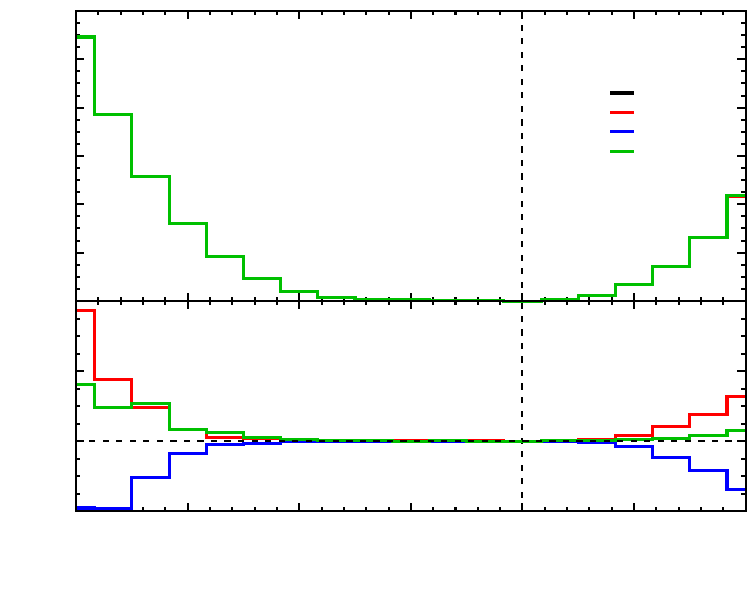
\includegraphics{pics/new_0_11a_11b_8_chi2_S23}}%
    \gplfronttext
  \end{picture}%
\endgroup
}
	\resizebox{0.49\linewidth}{!}{% GNUPLOT: LaTeX picture with Postscript
\begingroup
  \makeatletter
  \providecommand\color[2][]{%
    \GenericError{(gnuplot) \space\space\space\@spaces}{%
      Package color not loaded in conjunction with
      terminal option `colourtext'%
    }{See the gnuplot documentation for explanation.%
    }{Either use 'blacktext' in gnuplot or load the package
      color.sty in LaTeX.}%
    \renewcommand\color[2][]{}%
  }%
  \providecommand\includegraphics[2][]{%
    \GenericError{(gnuplot) \space\space\space\@spaces}{%
      Package graphicx or graphics not loaded%
    }{See the gnuplot documentation for explanation.%
    }{The gnuplot epslatex terminal needs graphicx.sty or graphics.sty.}%
    \renewcommand\includegraphics[2][]{}%
  }%
  \providecommand\rotatebox[2]{#2}%
  \@ifundefined{ifGPcolor}{%
    \newif\ifGPcolor
    \GPcolortrue
  }{}%
  \@ifundefined{ifGPblacktext}{%
    \newif\ifGPblacktext
    \GPblacktexttrue
  }{}%
  % define a \g@addto@macro without @ in the name:
  \let\gplgaddtomacro\g@addto@macro
  % define empty templates for all commands taking text:
  \gdef\gplbacktext{}%
  \gdef\gplfronttext{}%
  \makeatother
  \ifGPblacktext
    % no textcolor at all
    \def\colorrgb#1{}%
    \def\colorgray#1{}%
  \else
    % gray or color?
    \ifGPcolor
      \def\colorrgb#1{\color[rgb]{#1}}%
      \def\colorgray#1{\color[gray]{#1}}%
      \expandafter\def\csname LTw\endcsname{\color{white}}%
      \expandafter\def\csname LTb\endcsname{\color{black}}%
      \expandafter\def\csname LTa\endcsname{\color{black}}%
      \expandafter\def\csname LT0\endcsname{\color[rgb]{1,0,0}}%
      \expandafter\def\csname LT1\endcsname{\color[rgb]{0,1,0}}%
      \expandafter\def\csname LT2\endcsname{\color[rgb]{0,0,1}}%
      \expandafter\def\csname LT3\endcsname{\color[rgb]{1,0,1}}%
      \expandafter\def\csname LT4\endcsname{\color[rgb]{0,1,1}}%
      \expandafter\def\csname LT5\endcsname{\color[rgb]{1,1,0}}%
      \expandafter\def\csname LT6\endcsname{\color[rgb]{0,0,0}}%
      \expandafter\def\csname LT7\endcsname{\color[rgb]{1,0.3,0}}%
      \expandafter\def\csname LT8\endcsname{\color[rgb]{0.5,0.5,0.5}}%
    \else
      % gray
      \def\colorrgb#1{\color{black}}%
      \def\colorgray#1{\color[gray]{#1}}%
      \expandafter\def\csname LTw\endcsname{\color{white}}%
      \expandafter\def\csname LTb\endcsname{\color{black}}%
      \expandafter\def\csname LTa\endcsname{\color{black}}%
      \expandafter\def\csname LT0\endcsname{\color{black}}%
      \expandafter\def\csname LT1\endcsname{\color{black}}%
      \expandafter\def\csname LT2\endcsname{\color{black}}%
      \expandafter\def\csname LT3\endcsname{\color{black}}%
      \expandafter\def\csname LT4\endcsname{\color{black}}%
      \expandafter\def\csname LT5\endcsname{\color{black}}%
      \expandafter\def\csname LT6\endcsname{\color{black}}%
      \expandafter\def\csname LT7\endcsname{\color{black}}%
      \expandafter\def\csname LT8\endcsname{\color{black}}%
    \fi
  \fi
    \setlength{\unitlength}{0.0500bp}%
    \ifx\gptboxheight\undefined%
      \newlength{\gptboxheight}%
      \newlength{\gptboxwidth}%
      \newsavebox{\gptboxtext}%
    \fi%
    \setlength{\fboxrule}{0.5pt}%
    \setlength{\fboxsep}{1pt}%
\begin{picture}(7200.00,5760.00)%
    \gplgaddtomacro\gplbacktext{%
      \csname LTb\endcsname%%
      \put(747,927){\makebox(0,0)[r]{\strut{}2.47}}%
      \csname LTb\endcsname%%
      \put(747,1480){\makebox(0,0)[r]{\strut{}2.48}}%
      \csname LTb\endcsname%%
      \put(747,2033){\makebox(0,0)[r]{\strut{}2.49}}%
      \csname LTb\endcsname%%
      \put(747,2586){\makebox(0,0)[r]{\strut{}2.5}}%
      \csname LTb\endcsname%%
      \put(747,3139){\makebox(0,0)[r]{\strut{}2.51}}%
      \csname LTb\endcsname%%
      \put(747,3692){\makebox(0,0)[r]{\strut{}2.52}}%
      \csname LTb\endcsname%%
      \put(747,4246){\makebox(0,0)[r]{\strut{}2.53}}%
      \csname LTb\endcsname%%
      \put(747,4799){\makebox(0,0)[r]{\strut{}2.54}}%
      \csname LTb\endcsname%%
      \put(747,5352){\makebox(0,0)[r]{\strut{}2.55}}%
      \csname LTb\endcsname%%
      \put(1402,409){\makebox(0,0){\strut{}0.44}}%
      \csname LTb\endcsname%%
      \put(2192,409){\makebox(0,0){\strut{}0.46}}%
      \csname LTb\endcsname%%
      \put(2982,409){\makebox(0,0){\strut{}0.48}}%
      \csname LTb\endcsname%%
      \put(3772,409){\makebox(0,0){\strut{}0.5}}%
      \csname LTb\endcsname%%
      \put(4562,409){\makebox(0,0){\strut{}0.52}}%
      \csname LTb\endcsname%%
      \put(5352,409){\makebox(0,0){\strut{}0.54}}%
      \csname LTb\endcsname%%
      \put(6142,409){\makebox(0,0){\strut{}0.56}}%
      \csname LTb\endcsname%%
      \put(4915,3121){\makebox(0,0)[l]{\strut{}}}%
    }%
    \gplgaddtomacro\gplfronttext{%
      \csname LTb\endcsname%%
      \put(153,3084){\rotatebox{-270}{\makebox(0,0){\strut{}$\Delta m_{32}^2 / 10^{-3}$}}}%
      \csname LTb\endcsname%%
      \put(3871,130){\makebox(0,0){\strut{}$\sin^2 \theta_{23}$}}%
      \csname LTb\endcsname%%
      \put(6360,5406){\makebox(0,0)[r]{\strut{}0}}%
      \csname LTb\endcsname%%
      \put(6360,5220){\makebox(0,0)[r]{\strut{}11a}}%
      \csname LTb\endcsname%%
      \put(6360,5034){\makebox(0,0)[r]{\strut{}11b}}%
      \csname LTb\endcsname%%
      \put(6360,4848){\makebox(0,0)[r]{\strut{}8}}%
    }%
    \gplbacktext
    \put(0,0){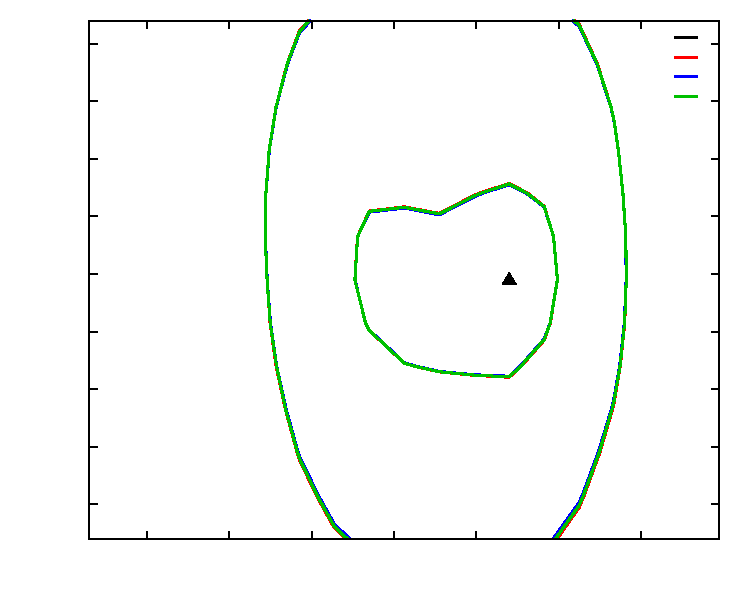
\includegraphics{pics/new_0_11a_11b_8_cont_S23_M23}}%
    \gplfronttext
  \end{picture}%
\endgroup
}	%%%%%%%%%%%this is important
	\resizebox{0.49\linewidth}{!}{% GNUPLOT: LaTeX picture with Postscript
\begingroup
  \makeatletter
  \providecommand\color[2][]{%
    \GenericError{(gnuplot) \space\space\space\@spaces}{%
      Package color not loaded in conjunction with
      terminal option `colourtext'%
    }{See the gnuplot documentation for explanation.%
    }{Either use 'blacktext' in gnuplot or load the package
      color.sty in LaTeX.}%
    \renewcommand\color[2][]{}%
  }%
  \providecommand\includegraphics[2][]{%
    \GenericError{(gnuplot) \space\space\space\@spaces}{%
      Package graphicx or graphics not loaded%
    }{See the gnuplot documentation for explanation.%
    }{The gnuplot epslatex terminal needs graphicx.sty or graphics.sty.}%
    \renewcommand\includegraphics[2][]{}%
  }%
  \providecommand\rotatebox[2]{#2}%
  \@ifundefined{ifGPcolor}{%
    \newif\ifGPcolor
    \GPcolortrue
  }{}%
  \@ifundefined{ifGPblacktext}{%
    \newif\ifGPblacktext
    \GPblacktexttrue
  }{}%
  % define a \g@addto@macro without @ in the name:
  \let\gplgaddtomacro\g@addto@macro
  % define empty templates for all commands taking text:
  \gdef\gplbacktext{}%
  \gdef\gplfronttext{}%
  \makeatother
  \ifGPblacktext
    % no textcolor at all
    \def\colorrgb#1{}%
    \def\colorgray#1{}%
  \else
    % gray or color?
    \ifGPcolor
      \def\colorrgb#1{\color[rgb]{#1}}%
      \def\colorgray#1{\color[gray]{#1}}%
      \expandafter\def\csname LTw\endcsname{\color{white}}%
      \expandafter\def\csname LTb\endcsname{\color{black}}%
      \expandafter\def\csname LTa\endcsname{\color{black}}%
      \expandafter\def\csname LT0\endcsname{\color[rgb]{1,0,0}}%
      \expandafter\def\csname LT1\endcsname{\color[rgb]{0,1,0}}%
      \expandafter\def\csname LT2\endcsname{\color[rgb]{0,0,1}}%
      \expandafter\def\csname LT3\endcsname{\color[rgb]{1,0,1}}%
      \expandafter\def\csname LT4\endcsname{\color[rgb]{0,1,1}}%
      \expandafter\def\csname LT5\endcsname{\color[rgb]{1,1,0}}%
      \expandafter\def\csname LT6\endcsname{\color[rgb]{0,0,0}}%
      \expandafter\def\csname LT7\endcsname{\color[rgb]{1,0.3,0}}%
      \expandafter\def\csname LT8\endcsname{\color[rgb]{0.5,0.5,0.5}}%
    \else
      % gray
      \def\colorrgb#1{\color{black}}%
      \def\colorgray#1{\color[gray]{#1}}%
      \expandafter\def\csname LTw\endcsname{\color{white}}%
      \expandafter\def\csname LTb\endcsname{\color{black}}%
      \expandafter\def\csname LTa\endcsname{\color{black}}%
      \expandafter\def\csname LT0\endcsname{\color{black}}%
      \expandafter\def\csname LT1\endcsname{\color{black}}%
      \expandafter\def\csname LT2\endcsname{\color{black}}%
      \expandafter\def\csname LT3\endcsname{\color{black}}%
      \expandafter\def\csname LT4\endcsname{\color{black}}%
      \expandafter\def\csname LT5\endcsname{\color{black}}%
      \expandafter\def\csname LT6\endcsname{\color{black}}%
      \expandafter\def\csname LT7\endcsname{\color{black}}%
      \expandafter\def\csname LT8\endcsname{\color{black}}%
    \fi
  \fi
    \setlength{\unitlength}{0.0500bp}%
    \ifx\gptboxheight\undefined%
      \newlength{\gptboxheight}%
      \newlength{\gptboxwidth}%
      \newsavebox{\gptboxtext}%
    \fi%
    \setlength{\fboxrule}{0.5pt}%
    \setlength{\fboxsep}{1pt}%
\begin{picture}(7200.00,5760.00)%
    \gplgaddtomacro\gplbacktext{%
      \csname LTb\endcsname%%
      \put(849,707){\makebox(0,0)[r]{\strut{}-1.0$\pi$}}%
      \csname LTb\endcsname%%
      \put(849,1499){\makebox(0,0)[r]{\strut{}-0.6$\pi$}}%
      \csname LTb\endcsname%%
      \put(849,2292){\makebox(0,0)[r]{\strut{}-0.3$\pi$}}%
      \csname LTb\endcsname%%
      \put(849,3084){\makebox(0,0)[r]{\strut{}0.0$\pi$}}%
      \csname LTb\endcsname%%
      \put(849,3876){\makebox(0,0)[r]{\strut{}0.3$\pi$}}%
      \csname LTb\endcsname%%
      \put(849,4669){\makebox(0,0)[r]{\strut{}0.6$\pi$}}%
      \csname LTb\endcsname%%
      \put(849,5461){\makebox(0,0)[r]{\strut{}1.0$\pi$}}%
      \csname LTb\endcsname%%
      \put(951,409){\makebox(0,0){\strut{}0.07}}%
      \csname LTb\endcsname%%
      \put(1941,409){\makebox(0,0){\strut{}0.075}}%
      \csname LTb\endcsname%%
      \put(2931,409){\makebox(0,0){\strut{}0.08}}%
      \csname LTb\endcsname%%
      \put(3921,409){\makebox(0,0){\strut{}0.085}}%
      \csname LTb\endcsname%%
      \put(4911,409){\makebox(0,0){\strut{}0.09}}%
      \csname LTb\endcsname%%
      \put(5901,409){\makebox(0,0){\strut{}0.095}}%
      \csname LTb\endcsname%%
      \put(6891,409){\makebox(0,0){\strut{}0.1}}%
      \csname LTb\endcsname%%
      \put(3970,1876){\makebox(0,0)[l]{\strut{}}}%
    }%
    \gplgaddtomacro\gplfronttext{%
      \csname LTb\endcsname%%
      \put(153,3084){\rotatebox{-270}{\makebox(0,0){\strut{}$\delta_\text{CP}$}}}%
      \csname LTb\endcsname%%
      \put(3922,130){\makebox(0,0){\strut{}$\sin^2 2 \theta_{13}$}}%
      \csname LTb\endcsname%%
      \put(6360,5406){\makebox(0,0)[r]{\strut{}0}}%
      \csname LTb\endcsname%%
      \put(6360,5220){\makebox(0,0)[r]{\strut{}11a}}%
      \csname LTb\endcsname%%
      \put(6360,5034){\makebox(0,0)[r]{\strut{}11b}}%
      \csname LTb\endcsname%%
      \put(6360,4848){\makebox(0,0)[r]{\strut{}8}}%
    }%
    \gplbacktext
    \put(0,0){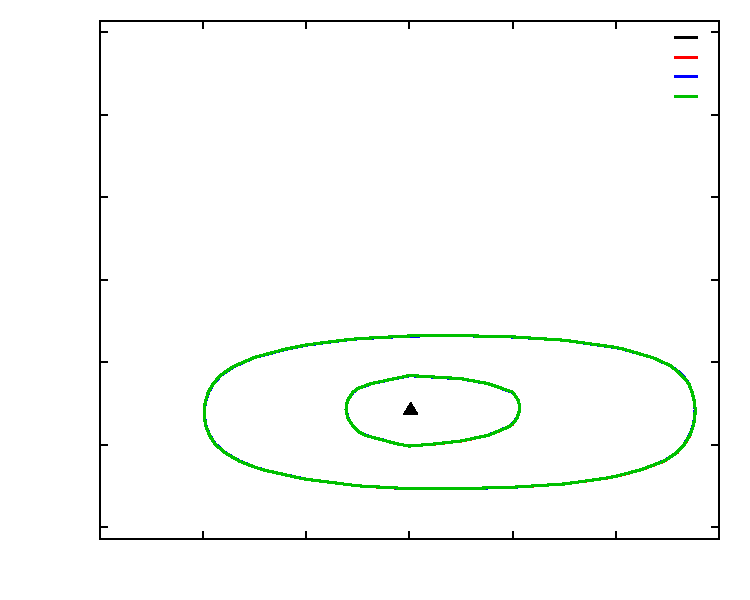
\includegraphics{pics/new_0_11a_11b_8_cont_S13_dCP}}%
    \gplfronttext
  \end{picture}%
\endgroup
}	%%%%%%%%%%%this is important
	\caption[$\chi^2$ profiles for $\delta_\text{CP}$, $\Delta m_{32}^2$, $\sin^2 2\theta_{13}$, and $\sin\theta_{23}$ %
		and contours for $\Delta m_{32}^2$ versus $\sin\theta_{23}$ and $\delta_\text{CP}$ versus $\sin^2 2\theta_{13}$ %
		with variations on the nominal systematic model]%
		{$\chi^2$ profile for $\delta_\text{CP}$ (top left), $\sin^2 2\theta_{13}$ (top right), %
		$\Delta m_{32}^2$ (middle left), and $\sin^2 \theta_{23}$ (middle right), %
		together with the contour levels for $\delta_\text{CP}$ versus $\sin^2 2\theta_{13}$ (bottom left) %
		and $\Delta m_{32}^2$ versus $\sin^2 \theta_{23}$ (bottom right).
		The bottom panels in the top four figures show the difference between the $\chi^2$ profiles computed %
		with the nominal model (\textbf{0}) and the variations of the nominal model itself %
		(\textbf{8}, \textbf{11a}, and \textbf{11b}).
		The dashed lines and the black triangles show the position of the best fit value, %
		which is always at the nominal Asimov A value.}
	\label{fig:0_11a_11b_8_profile}
\end{figure}

\begin{figure}
	\centering
	\resizebox{0.49\linewidth}{!}{% GNUPLOT: LaTeX picture with Postscript
\begingroup
  \makeatletter
  \providecommand\color[2][]{%
    \GenericError{(gnuplot) \space\space\space\@spaces}{%
      Package color not loaded in conjunction with
      terminal option `colourtext'%
    }{See the gnuplot documentation for explanation.%
    }{Either use 'blacktext' in gnuplot or load the package
      color.sty in LaTeX.}%
    \renewcommand\color[2][]{}%
  }%
  \providecommand\includegraphics[2][]{%
    \GenericError{(gnuplot) \space\space\space\@spaces}{%
      Package graphicx or graphics not loaded%
    }{See the gnuplot documentation for explanation.%
    }{The gnuplot epslatex terminal needs graphicx.sty or graphics.sty.}%
    \renewcommand\includegraphics[2][]{}%
  }%
  \providecommand\rotatebox[2]{#2}%
  \@ifundefined{ifGPcolor}{%
    \newif\ifGPcolor
    \GPcolortrue
  }{}%
  \@ifundefined{ifGPblacktext}{%
    \newif\ifGPblacktext
    \GPblacktexttrue
  }{}%
  % define a \g@addto@macro without @ in the name:
  \let\gplgaddtomacro\g@addto@macro
  % define empty templates for all commands taking text:
  \gdef\gplbacktext{}%
  \gdef\gplfronttext{}%
  \makeatother
  \ifGPblacktext
    % no textcolor at all
    \def\colorrgb#1{}%
    \def\colorgray#1{}%
  \else
    % gray or color?
    \ifGPcolor
      \def\colorrgb#1{\color[rgb]{#1}}%
      \def\colorgray#1{\color[gray]{#1}}%
      \expandafter\def\csname LTw\endcsname{\color{white}}%
      \expandafter\def\csname LTb\endcsname{\color{black}}%
      \expandafter\def\csname LTa\endcsname{\color{black}}%
      \expandafter\def\csname LT0\endcsname{\color[rgb]{1,0,0}}%
      \expandafter\def\csname LT1\endcsname{\color[rgb]{0,1,0}}%
      \expandafter\def\csname LT2\endcsname{\color[rgb]{0,0,1}}%
      \expandafter\def\csname LT3\endcsname{\color[rgb]{1,0,1}}%
      \expandafter\def\csname LT4\endcsname{\color[rgb]{0,1,1}}%
      \expandafter\def\csname LT5\endcsname{\color[rgb]{1,1,0}}%
      \expandafter\def\csname LT6\endcsname{\color[rgb]{0,0,0}}%
      \expandafter\def\csname LT7\endcsname{\color[rgb]{1,0.3,0}}%
      \expandafter\def\csname LT8\endcsname{\color[rgb]{0.5,0.5,0.5}}%
    \else
      % gray
      \def\colorrgb#1{\color{black}}%
      \def\colorgray#1{\color[gray]{#1}}%
      \expandafter\def\csname LTw\endcsname{\color{white}}%
      \expandafter\def\csname LTb\endcsname{\color{black}}%
      \expandafter\def\csname LTa\endcsname{\color{black}}%
      \expandafter\def\csname LT0\endcsname{\color{black}}%
      \expandafter\def\csname LT1\endcsname{\color{black}}%
      \expandafter\def\csname LT2\endcsname{\color{black}}%
      \expandafter\def\csname LT3\endcsname{\color{black}}%
      \expandafter\def\csname LT4\endcsname{\color{black}}%
      \expandafter\def\csname LT5\endcsname{\color{black}}%
      \expandafter\def\csname LT6\endcsname{\color{black}}%
      \expandafter\def\csname LT7\endcsname{\color{black}}%
      \expandafter\def\csname LT8\endcsname{\color{black}}%
    \fi
  \fi
    \setlength{\unitlength}{0.0500bp}%
    \ifx\gptboxheight\undefined%
      \newlength{\gptboxheight}%
      \newlength{\gptboxwidth}%
      \newsavebox{\gptboxtext}%
    \fi%
    \setlength{\fboxrule}{0.5pt}%
    \setlength{\fboxsep}{1pt}%
\begin{picture}(7200.00,5040.00)%
    \gplgaddtomacro\gplbacktext{%
      \csname LTb\endcsname%%
      \put(441,595){\makebox(0,0)[r]{\strut{}0}}%
      \csname LTb\endcsname%%
      \put(441,1660){\makebox(0,0)[r]{\strut{}2}}%
      \csname LTb\endcsname%%
      \put(441,2724){\makebox(0,0)[r]{\strut{}4}}%
      \csname LTb\endcsname%%
      \put(441,3789){\makebox(0,0)[r]{\strut{}6}}%
      \csname LTb\endcsname%%
      \put(441,4853){\makebox(0,0)[r]{\strut{}8}}%
      \csname LTb\endcsname%%
      \put(543,409){\makebox(0,0){\strut{}-1.0$\pi$}}%
      \csname LTb\endcsname%%
      \put(1337,409){\makebox(0,0){\strut{}-0.8$\pi$}}%
      \csname LTb\endcsname%%
      \put(2131,409){\makebox(0,0){\strut{}-0.5$\pi$}}%
      \csname LTb\endcsname%%
      \put(2924,409){\makebox(0,0){\strut{}-0.2$\pi$}}%
      \csname LTb\endcsname%%
      \put(3718,409){\makebox(0,0){\strut{}0.0$\pi$}}%
      \csname LTb\endcsname%%
      \put(4512,409){\makebox(0,0){\strut{}0.2$\pi$}}%
      \csname LTb\endcsname%%
      \put(5306,409){\makebox(0,0){\strut{}0.5$\pi$}}%
      \csname LTb\endcsname%%
      \put(6099,409){\makebox(0,0){\strut{}0.8$\pi$}}%
      \csname LTb\endcsname%%
      \put(6893,409){\makebox(0,0){\strut{}1.0$\pi$}}%
      \csname LTb\endcsname%%
      \put(3718,3522){\makebox(0,0){\strut{}$5 \sigma$}}%
      \csname LTb\endcsname%%
      \put(3718,2458){\makebox(0,0){\strut{}$3 \sigma$}}%
    }%
    \gplgaddtomacro\gplfronttext{%
      \csname LTb\endcsname%%
      \put(153,2724){\rotatebox{-270}{\makebox(0,0){\strut{}$\sigma (\delta_\text{CP})$}}}%
      \csname LTb\endcsname%%
      \put(3718,130){\makebox(0,0){\strut{}$\delta_\text{CP}$}}%
      \csname LTb\endcsname%%
      \put(1076,4686){\makebox(0,0)[l]{\strut{}0}}%
      \csname LTb\endcsname%%
      \put(1076,4500){\makebox(0,0)[l]{\strut{}11a}}%
      \csname LTb\endcsname%%
      \put(1076,4314){\makebox(0,0)[l]{\strut{}11b}}%
      \csname LTb\endcsname%%
      \put(1076,4128){\makebox(0,0)[l]{\strut{}8}}%
    }%
    \gplbacktext
    \put(0,0){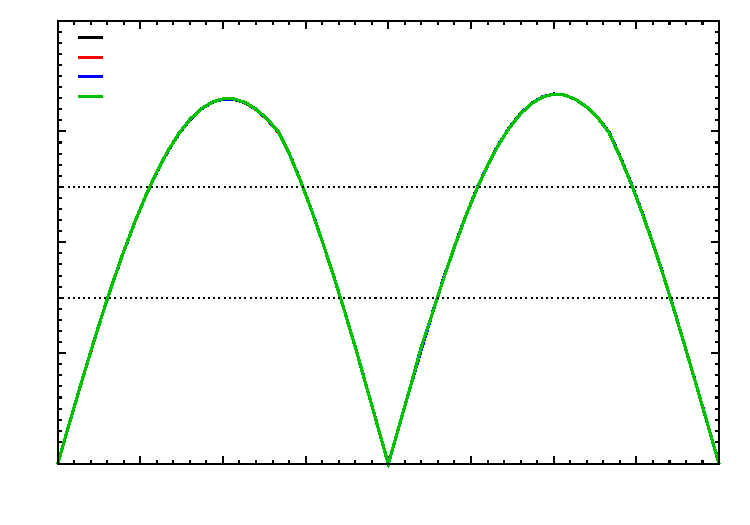
\includegraphics{pics/new_0_11a_11b_8_sensitivity}}%
    \gplfronttext
  \end{picture}%
\endgroup
}
	\resizebox{0.49\linewidth}{!}{% GNUPLOT: LaTeX picture with Postscript
\begingroup
  \makeatletter
  \providecommand\color[2][]{%
    \GenericError{(gnuplot) \space\space\space\@spaces}{%
      Package color not loaded in conjunction with
      terminal option `colourtext'%
    }{See the gnuplot documentation for explanation.%
    }{Either use 'blacktext' in gnuplot or load the package
      color.sty in LaTeX.}%
    \renewcommand\color[2][]{}%
  }%
  \providecommand\includegraphics[2][]{%
    \GenericError{(gnuplot) \space\space\space\@spaces}{%
      Package graphicx or graphics not loaded%
    }{See the gnuplot documentation for explanation.%
    }{The gnuplot epslatex terminal needs graphicx.sty or graphics.sty.}%
    \renewcommand\includegraphics[2][]{}%
  }%
  \providecommand\rotatebox[2]{#2}%
  \@ifundefined{ifGPcolor}{%
    \newif\ifGPcolor
    \GPcolortrue
  }{}%
  \@ifundefined{ifGPblacktext}{%
    \newif\ifGPblacktext
    \GPblacktexttrue
  }{}%
  % define a \g@addto@macro without @ in the name:
  \let\gplgaddtomacro\g@addto@macro
  % define empty templates for all commands taking text:
  \gdef\gplbacktext{}%
  \gdef\gplfronttext{}%
  \makeatother
  \ifGPblacktext
    % no textcolor at all
    \def\colorrgb#1{}%
    \def\colorgray#1{}%
  \else
    % gray or color?
    \ifGPcolor
      \def\colorrgb#1{\color[rgb]{#1}}%
      \def\colorgray#1{\color[gray]{#1}}%
      \expandafter\def\csname LTw\endcsname{\color{white}}%
      \expandafter\def\csname LTb\endcsname{\color{black}}%
      \expandafter\def\csname LTa\endcsname{\color{black}}%
      \expandafter\def\csname LT0\endcsname{\color[rgb]{1,0,0}}%
      \expandafter\def\csname LT1\endcsname{\color[rgb]{0,1,0}}%
      \expandafter\def\csname LT2\endcsname{\color[rgb]{0,0,1}}%
      \expandafter\def\csname LT3\endcsname{\color[rgb]{1,0,1}}%
      \expandafter\def\csname LT4\endcsname{\color[rgb]{0,1,1}}%
      \expandafter\def\csname LT5\endcsname{\color[rgb]{1,1,0}}%
      \expandafter\def\csname LT6\endcsname{\color[rgb]{0,0,0}}%
      \expandafter\def\csname LT7\endcsname{\color[rgb]{1,0.3,0}}%
      \expandafter\def\csname LT8\endcsname{\color[rgb]{0.5,0.5,0.5}}%
    \else
      % gray
      \def\colorrgb#1{\color{black}}%
      \def\colorgray#1{\color[gray]{#1}}%
      \expandafter\def\csname LTw\endcsname{\color{white}}%
      \expandafter\def\csname LTb\endcsname{\color{black}}%
      \expandafter\def\csname LTa\endcsname{\color{black}}%
      \expandafter\def\csname LT0\endcsname{\color{black}}%
      \expandafter\def\csname LT1\endcsname{\color{black}}%
      \expandafter\def\csname LT2\endcsname{\color{black}}%
      \expandafter\def\csname LT3\endcsname{\color{black}}%
      \expandafter\def\csname LT4\endcsname{\color{black}}%
      \expandafter\def\csname LT5\endcsname{\color{black}}%
      \expandafter\def\csname LT6\endcsname{\color{black}}%
      \expandafter\def\csname LT7\endcsname{\color{black}}%
      \expandafter\def\csname LT8\endcsname{\color{black}}%
    \fi
  \fi
    \setlength{\unitlength}{0.0500bp}%
    \ifx\gptboxheight\undefined%
      \newlength{\gptboxheight}%
      \newlength{\gptboxwidth}%
      \newsavebox{\gptboxtext}%
    \fi%
    \setlength{\fboxrule}{0.5pt}%
    \setlength{\fboxsep}{1pt}%
\begin{picture}(7200.00,5040.00)%
    \gplgaddtomacro\gplbacktext{%
      \csname LTb\endcsname%%
      \put(849,595){\makebox(0,0)[r]{\strut{}-0.01}}%
      \csname LTb\endcsname%%
      \put(849,2724){\makebox(0,0)[r]{\strut{}0}}%
      \csname LTb\endcsname%%
      \put(849,4853){\makebox(0,0)[r]{\strut{}0.01}}%
      \csname LTb\endcsname%%
      \put(951,409){\makebox(0,0){\strut{}-1.0$\pi$}}%
      \csname LTb\endcsname%%
      \put(1694,409){\makebox(0,0){\strut{}-0.8$\pi$}}%
      \csname LTb\endcsname%%
      \put(2437,409){\makebox(0,0){\strut{}-0.5$\pi$}}%
      \csname LTb\endcsname%%
      \put(3179,409){\makebox(0,0){\strut{}-0.2$\pi$}}%
      \csname LTb\endcsname%%
      \put(3922,409){\makebox(0,0){\strut{}0.0$\pi$}}%
      \csname LTb\endcsname%%
      \put(4665,409){\makebox(0,0){\strut{}0.2$\pi$}}%
      \csname LTb\endcsname%%
      \put(5408,409){\makebox(0,0){\strut{}0.5$\pi$}}%
      \csname LTb\endcsname%%
      \put(6150,409){\makebox(0,0){\strut{}0.8$\pi$}}%
      \csname LTb\endcsname%%
      \put(6893,409){\makebox(0,0){\strut{}1.0$\pi$}}%
    }%
    \gplgaddtomacro\gplfronttext{%
      \csname LTb\endcsname%%
      \put(153,2724){\rotatebox{-270}{\makebox(0,0){\strut{}$\sigma_0 - \sigma$}}}%
      \csname LTb\endcsname%%
      \put(3922,130){\makebox(0,0){\strut{}$\delta_\text{CP}$}}%
      \csname LTb\endcsname%%
      \put(1484,4686){\makebox(0,0)[l]{\strut{}11a}}%
      \csname LTb\endcsname%%
      \put(1484,4500){\makebox(0,0)[l]{\strut{}11b}}%
      \csname LTb\endcsname%%
      \put(1484,4314){\makebox(0,0)[l]{\strut{}8}}%
    }%
    \gplbacktext
    \put(0,0){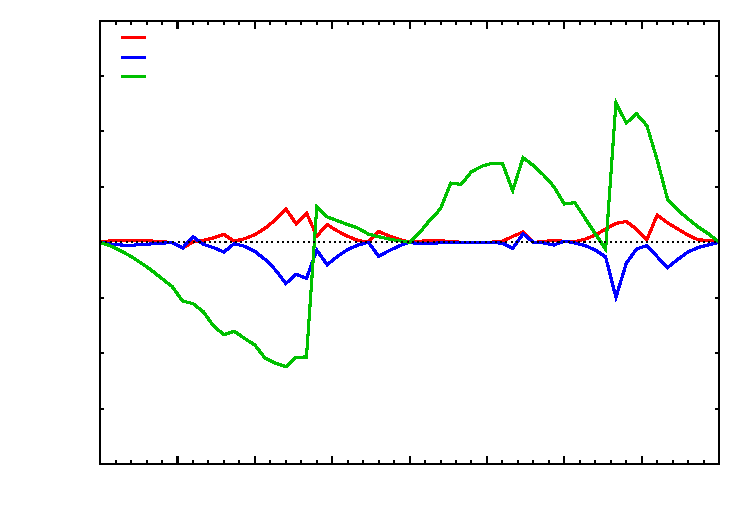
\includegraphics{pics/new_0_11a_11b_8_detail}}%
    \gplfronttext
  \end{picture}%
\endgroup
}
	\caption[Sensitivity to $\delta_\text{CP} = 0$ with variations on the nominal systematic model]%
		{Expected significance (right) to exclude CP conservation with the nominal model (\textbf{0}) %
		and its variations (\textbf{8}, \textbf{11a}, and \textbf{11b}).
		On the left, the difference of each curve with the nominal model show that the sensitivity %
		does not change significantly with the modifications of the systematic model in place.}
	\label{fig:0_11a_11b_8_sensitivity}
\end{figure}

